% The G17 technical reference.
% Build: latexmk -lualatex g17-technical-reference.tex   (from docs/tex)
\documentclass[11pt, letterpaper, oneside, open=any, numbers=noenddot]{scrreprt}
% Preamble for the G17 technical reference.
\usepackage{fontspec}
\usepackage{libertinus-otf}
\setmonofont{Inconsolatazi4}[Scale=MatchLowercase, ItalicFont=Inconsolatazi4, ItalicFeatures={FakeSlant=0.18}]
\usepackage{unicode-math}
\setmathfont{Libertinus Math}
\usepackage[final]{microtype}
\usepackage[english]{babel}
\usepackage[autostyle]{csquotes}
\MakeOuterQuote{"}

\usepackage[margin=1.05in, top=1in, bottom=1.1in]{geometry}
\usepackage{xcolor}
\definecolor{ink}{HTML}{1F2933}
\definecolor{accent}{HTML}{25569A}
\definecolor{apple}{HTML}{6B7280}
\definecolor{ours}{HTML}{1F5FA6}
\definecolor{native}{HTML}{B4462B}
\definecolor{rule}{HTML}{C9CED6}
\definecolor{codebg}{HTML}{F5F6F8}
\definecolor{hilite}{HTML}{F6D365}

\usepackage{enumitem}
\setlist{itemsep=2pt, topsep=0pt, parsep=0pt}
\setlist[itemize]{label=\textcolor{apple}{\textbullet}, leftmargin=1.4em}
\setlist[itemize,2]{label=\textcolor{apple}{\textendash}}

\usepackage{booktabs}
\usepackage{array}
\usepackage{longtable}
\usepackage{xltabular}
\renewcommand\tabularxcolumn[1]{>{\raggedright\arraybackslash}p{#1}}
\setlength{\LTpre}{9pt}
\setlength{\LTpost}{6pt}
\usepackage{etoolbox}
\newcommand{\tablesize}{\small}
% \widetable before a table with six or more columns sets it one size smaller.
\newcommand{\widetable}{\gdef\tablesize{\footnotesize}}
\AtBeginEnvironment{longtable}{\tablesize\renewcommand\arraystretch{1.12}\gdef\tablesize{\small}}
\AtBeginEnvironment{xltabular}{\tablesize\renewcommand\arraystretch{1.12}\gdef\tablesize{\small}}
\setlength{\extrarowheight}{1.5pt}
\setlength{\LTleft}{0pt}
\setlength{\LTright}{\fill}
\usepackage{seqsplit}

\usepackage{listings}
\lstset{basicstyle=\ttfamily\footnotesize, columns=fullflexible, keepspaces=true,
  breaklines=true, breakatwhitespace=false, backgroundcolor=\color{codebg},
  frame=none, xleftmargin=6pt, xrightmargin=6pt, framesep=4pt,
  aboveskip=8pt, belowskip=8pt, showstringspaces=false, upquote=true,
  extendedchars=true}
\lstdefinestyle{py}{language=Python, keywordstyle=\color{accent}\bfseries,
  commentstyle=\color{apple}\itshape, stringstyle=\color{native}}

\usepackage{tikz}
\usetikzlibrary{arrows.meta, positioning, fit, backgrounds, calc, shapes.misc, decorations.pathreplacing}
\usepackage{bytefield}
\bytefieldsetup{bitformatting=\footnotesize}
\usepackage{caption}
\captionsetup{font=small, labelfont=bf, format=plain, labelsep=period, justification=raggedright,
  singlelinecheck=false, margin=0pt}
\usepackage[most]{tcolorbox}

% Chapter-number sections in the opening (0.1, 0.2, ...).
\KOMAoptions{parskip=half-}
\setkomafont{disposition}{\normalfont\bfseries\color{ink}}
\setkomafont{part}{\normalfont\Huge\bfseries\color{ink}}
\setkomafont{chapter}{\normalfont\huge\bfseries\color{ink}}
\RedeclareSectionCommand[beforeskip=0pt, afterskip=1.2\baselineskip]{chapter}
\RedeclareSectionCommand[tocnumwidth=2.6em]{section}
\setkomafont{title}{\normalfont\bfseries\color{ink}}
\setkomafont{subtitle}{\normalfont\large\color{ink!80}}
\RedeclareSectionCommand[beforeskip=-1.4\baselineskip, afterskip=0.5\baselineskip]{section}
\RedeclareSectionCommand[beforeskip=-1.0\baselineskip, afterskip=0.3\baselineskip, font=\normalsize\bfseries]{subsection}
\setcounter{secnumdepth}{1}
\setcounter{tocdepth}{1}
\counterwithout{figure}{chapter}
\renewcommand{\thefigure}{\thechapter.\arabic{figure}}
\counterwithin{figure}{chapter}
\counterwithin{table}{chapter}
\captionsetup[table]{position=top, skip=4pt}
% A table's caption row: \caption{...}\label{tab:...}\\ before \toprule. The header is repeated under a
% "continued" line when a long table breaks across pages.
\newcommand{\tablecontinued}[1]{\multicolumn{#1}{@{}l@{}}{\footnotesize\itshape\tablename~\thetable, continued}\\}

\usepackage[hyphens]{url}
\usepackage[colorlinks=true, linkcolor=accent, urlcolor=accent, citecolor=accent, linktoc=page,
  pdftitle={The G17 technical reference}, bookmarksnumbered=true]{hyperref}
\usepackage{bookmark}
% Cross-references: \cref{x} prints "section 10.4", "chapter 9", "appendix C" or "figure 3.1" from the label's
% own type, so the word cannot go stale; \Cref at the start of a sentence; \crefrange{a}{b} for "sections 2.4 to 2.6".
\usepackage[nameinlink, noabbrev]{cleveref}
\crefname{part}{Part}{Parts}
\crefname{chapter}{chapter}{chapters}
\crefname{section}{section}{sections}
\crefname{appendix}{appendix}{appendices}
\crefname{figure}{figure}{figures}
\crefname{table}{table}{tables}
\newcommand{\crefrangeconjunction}{ to~}
\pdfstringdefDisableCommands{\def\_{_}\def\code#1{#1}\def\op#1{op#1}\def\Op#1{op#1}\def\opn#1{op#1}\def\val#1{#1}}

% --- Semantic macros -------------------------------------------------------
% Inline code may break after / . _ , ; : ( and before =, so long paths and
% identifiers do not run into the margin.
\usepackage{luacode}
\begin{luacode*}
function g17_code(s)
  local long = #s > 16
  s = s:gsub('"', '\0Q')
  s = s:gsub('\\_ ?', '\0U'):gsub('\\%& ?', '\0A'):gsub('\\%# ?', '\0H'):gsub('\\%$ ?', '\0D')
  s = s:gsub('\\%% ?', '\0P'):gsub('\\{ ?', '\0L'):gsub('\\} ?', '\0R')
  s = s:gsub('\\textbackslash ?{}', '\0B'):gsub('\\textasciicircum ?{}', '\0C'):gsub('\\textasciitilde ?{}', '\0T')
  s = s:gsub('([/,;])', '%1\0Z')
  if long then
    s = s:gsub('%z(U)', '\0V')
    s = s:gsub('([%.|(])', '%1\0Z')
    s = s:gsub('%zZ(%a%a?%a?%a?)$', '%1')   -- no break before a file extension
  end
  if #s > 30 then s = s:gsub('(%l%l%l)(%u%l%l)', '%1\0Z%2') end
  local m = {U='\\textunderscore{}', V='\\textunderscore\\allowbreak{}', Q='\\textquotedbl{}', A='\\&', H='\\#', D='\\$', P='\\%', L='\\{', R='\\}',
             B='\\textbackslash{}', C='\\textasciicircum{}', T='\\textasciitilde{}', Z='\\allowbreak{}'}
  s = s:gsub('%z(%u)', m)
  tex.sprint(s)
end
\end{luacode*}
\DeclareRobustCommand{\code}[1]{\texttt{\exhyphenpenalty=10000\hyphenchar\font=-1 \directlua{g17_code("\luaescapestring{\detokenize{#1}}")}}}
\emergencystretch=3em
\widowpenalty=10000
\clubpenalty=10000
\usepackage{needspace}
% Keep a heading with at least a few lines of what follows it.
\AddToHook{cmd/section/before}{\Needspace{7\baselineskip}}
\AddToHook{cmd/subsection/before}{\Needspace{5\baselineskip}}
% A bold run-in line that introduces a list or table stays with it.
\newcommand{\leadhead}[1]{\Needspace{4\baselineskip}\noindent\textbf{#1}\par\nopagebreak}
\makeatletter
\setlength{\@fptop}{0pt}
\makeatother
\renewcommand{\floatpagefraction}{0.75}
\renewcommand{\topfraction}{0.85}
\renewcommand{\textfraction}{0.1}
\newcommand{\hash}[1]{\texttt{\seqsplit{#1}}}

% Opcodes name themselves. \op{5107} prints the glossary name and the number, linked to the opcode's row in
% appendix C; \Op{5107} capitalizes the name at a sentence start; \opn{5107} prints the linked number alone (a
% table cell beside a name column, or a deliberately shortened name); \opdef{5107} makes the row. The names come
% from opnames.tex, generated from isa/g17-opcode-glossary.json by tools/g17docs.py --write-opnames. An opcode
% with no glossary entry prints its number only, and its paragraph says "no glossary entry".
\newcommand{\opnamedef}[3]{\expandafter\def\csname opname@#1\endcsname{#2}%
  \expandafter\def\csname Opname@#1\endcsname{#3}}
\DeclareRobustCommand{\opn}[1]{\hyperlink{op:#1}{\textcolor{ink}{\texttt{op#1}}}}
\DeclareRobustCommand{\op}[1]{\ifcsname opname@#1\endcsname\csname opname@#1\endcsname\ (\opn{#1})\else\opn{#1}\fi}
\DeclareRobustCommand{\Op}[1]{\ifcsname Opname@#1\endcsname\csname Opname@#1\endcsname\ (\opn{#1})\else\opn{#1}\fi}
\newcommand{\opdef}[1]{\hypertarget{op:#1}{\texttt{op#1}}}
% GENERATED by tools/g17docs.py --write-opnames from isa/g17-opcode-glossary.json; do not edit.
% \op{N} prints the name and the linked number; an opcode with no entry prints the number only.
\opnamedef{0}{uniform register file, decoder tag}{Uniform register file, decoder tag}
\opnamedef{4}{message staging file, decoder tag}{Message staging file, decoder tag}
\opnamedef{423}{32-bit AND with immediate}{32-bit AND with immediate}
\opnamedef{424}{32-bit AND}{32-bit AND}
\opnamedef{426}{16-bit AND with immediate, 32-bit result}{16-bit AND with immediate, 32-bit result}
\opnamedef{428}{16-bit AND, 32-bit result}{16-bit AND, 32-bit result}
\opnamedef{435}{16-bit AND with immediate}{16-bit AND with immediate}
\opnamedef{437}{16-bit AND}{16-bit AND}
\opnamedef{441}{32-bit AND with immediate into the uniform/staging file}{32-bit AND with immediate into the uniform/staging file}
\opnamedef{447}{threadgroup barrier}{Threadgroup barrier}
\opnamedef{450}{call}{Call}
\opnamedef{458}{conditional back-edge branch}{Conditional back-edge branch}
\opnamedef{462}{skip branch, no active lanes}{Skip branch, no active lanes}
\opnamedef{465}{population count}{Population count}
\opnamedef{554}{move immediate, two-operand form}{Move immediate, two-operand form}
\opnamedef{555}{16-bit move immediate into a half}{16-bit move immediate into a half}
\opnamedef{577}{exec pop, restore mask}{Exec pop, restore mask}
\opnamedef{579}{while-exec, set mask in place}{While-exec, set mask in place}
\opnamedef{580}{return}{Return}
\opnamedef{582}{exec push, if, from flag}{Exec push, if, from flag}
\opnamedef{586}{32-bit register move}{32-bit register move}
\opnamedef{590}{16-bit register move}{16-bit register move}
\opnamedef{592}{uniform / staging write}{Uniform / staging write}
\opnamedef{593}{publish sibling, function unknown}{Publish sibling, function unknown}
\opnamedef{595}{fragment spill store}{Fragment spill store}
\opnamedef{612}{range mask, immediate width}{Range mask, immediate width}
\opnamedef{615}{range mask, register width}{Range mask, register width}
\opnamedef{621}{range mask, 16-bit source}{Range mask, 16-bit source}
\opnamedef{684}{end of program}{End of program}
\opnamedef{776}{half add with float immediate}{Half add with float immediate}
\opnamedef{798}{fp16 fma, register form}{Fp16 fma, register form}
\opnamedef{838}{legacy 8×8 simdgroup MMA, f16}{Legacy 8×8 simdgroup MMA, f16}
\opnamedef{839}{legacy 8×8 simdgroup multiply, f16}{Legacy 8×8 simdgroup multiply, f16}
\opnamedef{904}{fp32 saturate}{Fp32 saturate}
\opnamedef{998}{fp32 add}{Fp32 add}
\opnamedef{1001}{fp32 add, rare alternate encoding}{Fp32 add, rare alternate encoding}
\opnamedef{1004}{half to fp32 widening}{Half to fp32 widening}
\opnamedef{1006}{fp32 add with float immediate}{Fp32 add with float immediate}
\opnamedef{1014}{fp32 add, half result}{Fp32 add, half result}
\opnamedef{1015}{fp32 plus half, half result}{Fp32 plus half, half result}
\opnamedef{1016}{fp32 to half narrowing}{Fp32 to half narrowing}
\opnamedef{1038}{fp32 add with immediate into the uniform/staging file}{Fp32 add with immediate into the uniform/staging file}
\opnamedef{1048}{fp32 to bfloat16 narrowing, unconfirmed}{Fp32 to bfloat16 narrowing, unconfirmed}
\opnamedef{1061}{fp32 add, common alternate encoding}{Fp32 add, common alternate encoding}
\opnamedef{1062}{fine x-derivative, saturated}{Fine x-derivative, saturated}
\opnamedef{1272}{hardware exp2}{Hardware exp2}
\opnamedef{2190}{fp32 fused multiply-add}{Fp32 fused multiply-add}
\opnamedef{2192}{fp32 FMA, literal addend}{Fp32 FMA, literal addend}
\opnamedef{2198}{fp32 FMA, literal multiplicand}{Fp32 FMA, literal multiplicand}
\opnamedef{2200}{fp32 FMA with two float immediates}{Fp32 FMA with two float immediates}
\opnamedef{2238}{fp32 fused multiply-add, alternate encoding}{Fp32 fused multiply-add, alternate encoding}
\opnamedef{2240}{FMA-family variant, narrow operand, unconfirmed}{FMA-family variant, narrow operand, unconfirmed}
\opnamedef{2241}{fused multiply-add, schedclass-87 base form}{Fused multiply-add, schedclass-87 base form}
\opnamedef{2318}{fp32 FMA into the uniform/staging file}{Fp32 FMA into the uniform/staging file}
\opnamedef{2433}{fused multiply-add, narrowed form}{Fused multiply-add, narrowed form}
\opnamedef{2570}{hardware log2}{Hardware log2}
\opnamedef{2842}{legacy 8×8 simdgroup MMA, fp32}{Legacy 8×8 simdgroup MMA, fp32}
\opnamedef{2844}{legacy 8×8 simdgroup multiply, fp32}{Legacy 8×8 simdgroup multiply, fp32}
\opnamedef{2862}{legacy 8×8 simdgroup MMA, f16 in fp32 out}{Legacy 8×8 simdgroup MMA, f16 in fp32 out}
\opnamedef{2902}{legacy 8×8 simdgroup MMA, bf16}{Legacy 8×8 simdgroup MMA, bf16}
\opnamedef{3290}{fp32 multiply}{Fp32 multiply}
\opnamedef{3291}{fp32 times half multiply}{Fp32 times half multiply}
\opnamedef{3298}{fp32 op with float immediate, unconfirmed}{Fp32 op with float immediate, unconfirmed}
\opnamedef{3306}{fp32 multiply, half result}{Fp32 multiply, half result}
\opnamedef{3322}{fp32 multiply into the uniform/staging file}{Fp32 multiply into the uniform/staging file}
\opnamedef{3653}{16-bit reciprocal into the uniform/staging file}{16-bit reciprocal into the uniform/staging file}
\opnamedef{3658}{hardware reciprocal}{Hardware reciprocal}
\opnamedef{3770}{round to nearest even}{Round to nearest even}
\opnamedef{3786}{floor}{Floor}
\opnamedef{3818}{fp32 truncate toward zero}{Fp32 truncate toward zero}
\opnamedef{3850}{rsqrt seed}{Rsqrt seed}
\opnamedef{3946}{trig-family op, function unmeasured}{Trig-family op, function unmeasured}
\opnamedef{3978}{sqrt-safe rsqrt}{Sqrt-safe rsqrt}
\opnamedef{5098}{tensor MMA, fp32 × fp32, accumulate}{Tensor MMA, fp32 × fp32, accumulate}
\opnamedef{5099}{tensor MMA, fp32 × fp32, no accumulator}{Tensor MMA, fp32 × fp32, no accumulator}
\opnamedef{5100}{tensor MMA, fp32 A × 16-bit B, accumulate}{Tensor MMA, fp32 A × 16-bit B, accumulate}
\opnamedef{5101}{tensor MMA, fp32 A × 16-bit B, no accumulator}{Tensor MMA, fp32 A × 16-bit B, no accumulator}
\opnamedef{5104}{tensor MMA, 16-bit A × fp32 B, accumulate}{Tensor MMA, 16-bit A × fp32 B, accumulate}
\opnamedef{5105}{tensor MMA, 16-bit A × fp32 B, no accumulator}{Tensor MMA, 16-bit A × fp32 B, no accumulator}
\opnamedef{5106}{tensor MMA, 16-bit × 16-bit, accumulate}{Tensor MMA, 16-bit × 16-bit, accumulate}
\opnamedef{5107}{tensor MMA, 16-bit × 16-bit, no accumulator}{Tensor MMA, 16-bit × 16-bit, no accumulator}
\opnamedef{5108}{table-only narrow-accumulator MMA, first}{Table-only narrow-accumulator MMA, first}
\opnamedef{5143}{table-only narrow-accumulator MMA, last, no accumulator}{Table-only narrow-accumulator MMA, last, no accumulator}
\opnamedef{9320}{fp32 to 32-bit integer}{Fp32 to 32-bit integer}
\opnamedef{9321}{half to 32-bit integer}{Half to 32-bit integer}
\opnamedef{9325}{half to 16-bit integer}{Half to 16-bit integer}
\opnamedef{9328}{fp32 to u32 into the uniform/staging file}{Fp32 to u32 into the uniform/staging file}
\opnamedef{9329}{half to 32-bit integer into the uniform/staging file}{Half to 32-bit integer into the uniform/staging file}
\opnamedef{9683}{half compare, chained into a flag}{Half compare, chained into a flag}
\opnamedef{9700}{fp32 compare-select, fmax/fmin}{Fp32 compare-select, fmax/fmin}
\opnamedef{9721}{32-bit compare-select, immediate arms}{32-bit compare-select, immediate arms}
\opnamedef{9748}{float compare-select, fselect form}{Float compare-select, fselect form}
\opnamedef{9749}{float compare-select, csel form}{Float compare-select, csel form}
\opnamedef{9832}{half compare-select}{Half compare-select}
\opnamedef{9842}{half compare-select against minifloat}{Half compare-select against minifloat}
\opnamedef{9986}{find most significant bit}{Find most significant bit}
\opnamedef{9989}{msb bit scan, 16-bit result}{Msb bit scan, 16-bit result}
\opnamedef{9996}{64-bit no-return atomic, max/min}{64-bit no-return atomic, max/min}
\opnamedef{10019}{per-lane-address no-return atomic}{Per-lane-address no-return atomic}
\opnamedef{10022}{uniform-address no-return atomic, 32-bit}{Uniform-address no-return atomic, 32-bit}
\opnamedef{10023}{uniform-address no-return compare-exchange}{Uniform-address no-return compare-exchange}
\opnamedef{10090}{per-lane-address atomic, returning}{Per-lane-address atomic, returning}
\opnamedef{10091}{per-lane-address compare-exchange, returning}{Per-lane-address compare-exchange, returning}
\opnamedef{10094}{uniform-address atomic, returning old}{Uniform-address atomic, returning old}
\opnamedef{10095}{uniform-address compare-exchange, returning}{Uniform-address compare-exchange, returning}
\opnamedef{10239}{32-bit saturating add}{32-bit saturating add}
\opnamedef{10267}{64-bit add}{64-bit add}
\opnamedef{10279}{32-bit add immediate}{32-bit add immediate}
\opnamedef{10282}{32-bit add}{32-bit add}
\opnamedef{10283}{add, 32-bit plus zero-extended 16-bit}{Add, 32-bit plus zero-extended 16-bit}
\opnamedef{10285}{add 16-bit to 32-bit}{Add 16-bit to 32-bit}
\opnamedef{10286}{16-bit plus 16-bit, 32-bit result}{16-bit plus 16-bit, 32-bit result}
\opnamedef{10289}{16-bit add immediate}{16-bit add immediate}
\opnamedef{10298}{32-bit add immediate into the uniform/staging file}{32-bit add immediate into the uniform/staging file}
\opnamedef{10306}{32-bit add into the uniform/staging file}{32-bit add into the uniform/staging file}
\opnamedef{10369}{32-bit compare with immediate into a flag}{32-bit compare with immediate into a flag}
\opnamedef{10372}{16-bit compare into a flag}{16-bit compare into a flag}
\opnamedef{10374}{16-bit register compare into a flag}{16-bit register compare into a flag}
\opnamedef{10378}{32-bit compare with immediate into a flag, short form}{32-bit compare with immediate into a flag, short form}
\opnamedef{10384}{tensor MMA, int8 widening to int32}{Tensor MMA, int8 widening to int32}
\opnamedef{10385}{tensor MMA, int8 widening, no accumulator}{Tensor MMA, int8 widening, no accumulator}
\opnamedef{10789}{32 × immediate to 64-bit product}{32 × immediate to 64-bit product}
\opnamedef{10790}{64-bit address multiply-add}{64-bit address multiply-add}
\opnamedef{10793}{32 × 32 to 64-bit product}{32 × 32 to 64-bit product}
\opnamedef{10795}{32 × 32 + 32 to 64-bit multiply-add}{32 × 32 + 32 to 64-bit multiply-add}
\opnamedef{10823}{multiply by immediate, 32-bit addend}{Multiply by immediate, 32-bit addend}
\opnamedef{10824}{multiply by immediate, 16-bit addend}{Multiply by immediate, 16-bit addend}
\opnamedef{10825}{32-bit multiply}{32-bit multiply}
\opnamedef{10826}{32-bit multiply-add}{32-bit multiply-add}
\opnamedef{10829}{multiply-add, 16-bit multiplier}{Multiply-add, 16-bit multiplier}
\opnamedef{10830}{multiply-add, 16-bit multiplier and addend}{Multiply-add, 16-bit multiplier and addend}
\opnamedef{10831}{16-bit multiply by immediate plus immediate}{16-bit multiply by immediate plus immediate}
\opnamedef{10835}{multiply-add, 16-bit multiplicand}{Multiply-add, 16-bit multiplicand}
\opnamedef{10836}{multiply-add, 16-bit multiplicand and addend}{Multiply-add, 16-bit multiplicand and addend}
\opnamedef{10838}{signed-by-unsigned 16-bit multiply-add}{Signed-by-unsigned 16-bit multiply-add}
\opnamedef{10858}{16-bit multiply by immediate plus immediate, 16-bit result}{16-bit multiply by immediate plus immediate, 16-bit result}
\opnamedef{10860}{16-bit multiply by immediate plus register}{16-bit multiply by immediate plus register}
\opnamedef{10879}{multiply by immediate plus immediate into the uniform/staging file}{Multiply by immediate plus immediate into the uniform/staging file}
\opnamedef{10883}{32-bit multiply into the uniform/staging file}{32-bit multiply into the uniform/staging file}
\opnamedef{10904}{MMA bit-flip mutation artifact}{MMA bit-flip mutation artifact}
\opnamedef{10909}{texture write}{Texture write}
\opnamedef{11059}{multiply by immediate minus immediate}{Multiply by immediate minus immediate}
\opnamedef{11060}{multiply by immediate minus register}{Multiply by immediate minus register}
\opnamedef{11063}{multiply-subtract}{Multiply-subtract}
\opnamedef{11120}{multiply-add into the uniform/staging file}{Multiply-add into the uniform/staging file}
\opnamedef{11179}{32-bit integer to fp32}{32-bit integer to fp32}
\opnamedef{11180}{16-bit integer to fp32}{16-bit integer to fp32}
\opnamedef{11182}{u32 to half}{U32 to half}
\opnamedef{11183}{16-bit integer to half}{16-bit integer to half}
\opnamedef{11185}{integer to float into the uniform/staging file}{Integer to float into the uniform/staging file}
\opnamedef{11190}{32-bit NOT}{32-bit NOT}
\opnamedef{11193}{NOT to 16-bit result}{NOT to 16-bit result}
\opnamedef{11196}{32-bit NOT into the uniform/staging file}{32-bit NOT into the uniform/staging file}
\opnamedef{11310}{32-bit compare, AND-chained into a flag}{32-bit compare, AND-chained into a flag}
\opnamedef{11313}{32-bit compare, OR-chained into a flag}{32-bit compare, OR-chained into a flag}
\opnamedef{11314}{32-bit compare, AND-chained into a flag with false arm}{32-bit compare, AND-chained into a flag with false arm}
\opnamedef{11322}{16-bit compare, chained into a flag}{16-bit compare, chained into a flag}
\opnamedef{11362}{32-bit compare-select against immediate}{32-bit compare-select against immediate}
\opnamedef{11364}{integer clamp}{Integer clamp}
\opnamedef{11365}{32-bit compare-select, three registers}{32-bit compare-select, three registers}
\opnamedef{11372}{32-bit register compare-select, immediate arms}{32-bit register compare-select, immediate arms}
\opnamedef{11375}{32-bit compare-select, four registers}{32-bit compare-select, four registers}
\opnamedef{11392}{16-bit compare-select against immediate, 32-bit result}{16-bit compare-select against immediate, 32-bit result}
\opnamedef{11415}{16-bit compare float select}{16-bit compare float select}
\opnamedef{11456}{32-bit compare against immediate, select to 16-bit}{32-bit compare against immediate, select to 16-bit}
\opnamedef{11458}{32-bit compare against immediate, select to 16-bit, minifloat false arm}{32-bit compare against immediate, select to 16-bit, minifloat false arm}
\opnamedef{11460}{32-bit compare against immediate, select to 16-bit, register false arm}{32-bit compare against immediate, select to 16-bit, register false arm}
\opnamedef{11461}{32-bit compare against immediate to half boolean}{32-bit compare against immediate to half boolean}
\opnamedef{11462}{32-bit register compare to 16-bit result}{32-bit register compare to 16-bit result}
\opnamedef{11466}{32-bit register compare, select to 16-bit}{32-bit register compare, select to 16-bit}
\opnamedef{11471}{32-bit register compare to half boolean}{32-bit register compare to half boolean}
\opnamedef{11472}{32-bit vs 16-bit compare to 16-bit result}{32-bit vs 16-bit compare to 16-bit result}
\opnamedef{11482}{16-bit compare-select against immediate}{16-bit compare-select against immediate}
\opnamedef{11491}{16-bit compare against immediate to half boolean}{16-bit compare against immediate to half boolean}
\opnamedef{11507}{16-bit compare-select, four registers}{16-bit compare-select, four registers}
\opnamedef{11564}{texture-coordinate staging write}{Texture-coordinate staging write}
\opnamedef{11624}{32-bit saturating subtract}{32-bit saturating subtract}
\opnamedef{11655}{64-bit subtract immediate}{64-bit subtract immediate}
\opnamedef{11666}{32-bit subtract immediate}{32-bit subtract immediate}
\opnamedef{11667}{32-bit subtract}{32-bit subtract}
\opnamedef{11689}{32-bit subtract immediate into the uniform/staging file}{32-bit subtract immediate into the uniform/staging file}
\opnamedef{11701}{threadgroup atomic, no return}{Threadgroup atomic, no return}
\opnamedef{11765}{threadgroup atomic, returning old}{Threadgroup atomic, returning old}
\opnamedef{11842}{move immediate, three-operand form}{Move immediate, three-operand form}
\opnamedef{11994}{ray-tracing block load, 32-bit}{Ray-tracing block load, 32-bit}
\opnamedef{12073}{device load, register address}{Device load, register address}
\opnamedef{12074}{device load, 16-bit register address}{Device load, 16-bit register address}
\opnamedef{12151}{imageblock load, 32-bit}{Imageblock load, 32-bit}
\opnamedef{12352}{MMA operand load, space unconfirmed}{MMA operand load, space unconfirmed}
\opnamedef{12364}{threadgroup-memory load}{Threadgroup-memory load}
\opnamedef{12397}{load, a further form}{Load, a further form}
\opnamedef{12646}{16-bit load}{16-bit load}
\opnamedef{12655}{packed half2 load}{Packed half2 load}
\opnamedef{12656}{int8 tensor load, one word}{Int8 tensor load, one word}
\opnamedef{12657}{masked int8 tensor load}{Masked int8 tensor load}
\opnamedef{12673}{plain 64-bit load, pair address}{Plain 64-bit load, pair address}
\opnamedef{12674}{tensor load, half/bf16}{Tensor load, half/bf16}
\opnamedef{12675}{masked tensor load, half/bf16}{Masked tensor load, half/bf16}
\opnamedef{12682}{plain 32-bit load}{Plain 32-bit load}
\opnamedef{12688}{immediate-address one-word load}{Immediate-address one-word load}
\opnamedef{12691}{plain 64-bit load}{Plain 64-bit load}
\opnamedef{12692}{tensor load, fp32}{Tensor load, fp32}
\opnamedef{12693}{masked tensor load, fp32}{Masked tensor load, fp32}
\opnamedef{12697}{immediate-address two-word load}{Immediate-address two-word load}
\opnamedef{12700}{three-component vector load}{Three-component vector load}
\opnamedef{12706}{immediate-address three-word load}{Immediate-address three-word load}
\opnamedef{12709}{128-bit vector load}{128-bit vector load}
\opnamedef{12715}{immediate-address four-word load}{Immediate-address four-word load}
\opnamedef{13075}{imageblock store, 32-bit}{Imageblock store, 32-bit}
\opnamedef{13276}{dequantized-block store, likely threadgroup}{Dequantized-block store, likely threadgroup}
\opnamedef{13288}{threadgroup-memory store}{Threadgroup-memory store}
\opnamedef{13483}{two-byte filler}{Two-byte filler}
\opnamedef{13574}{32-bit OR with immediate, seven-bit destination}{32-bit OR with immediate, seven-bit destination}
\opnamedef{13575}{32-bit OR}{32-bit OR}
\opnamedef{13576}{OR with 16-bit operand}{OR with 16-bit operand}
\opnamedef{13588}{16-bit OR}{16-bit OR}
\opnamedef{13592}{32-bit OR with immediate into the uniform/staging file}{32-bit OR with immediate into the uniform/staging file}
\opnamedef{13597}{16-bit OR into the uniform/staging file}{16-bit OR into the uniform/staging file}
\opnamedef{13618}{fp8 pack, vector, from fp32/half/bf16}{Fp8 pack, vector, from fp32/half/bf16}
\opnamedef{13620}{fp8 pack, scalar, from fp32}{Fp8 pack, scalar, from fp32}
\opnamedef{13754}{camera/video kernel op, function unknown}{Camera/video kernel op, function unknown}
\opnamedef{13856}{quad prefix sum, fp32}{Quad prefix sum, fp32}
\opnamedef{13944}{quad shuffle-xor, immediate mask}{Quad shuffle-xor, immediate mask}
\opnamedef{13945}{quad shuffle-xor, runtime mask}{Quad shuffle-xor, runtime mask}
\opnamedef{14047}{bit reverse}{Bit reverse}
\opnamedef{14059}{special-register read}{Special-register read}
\opnamedef{14060}{special-register read, 16-bit}{Special-register read, 16-bit}
\opnamedef{14061}{argument read, binding-table word}{Argument read, binding-table word}
\opnamedef{14099}{flag to 16-bit register}{Flag to 16-bit register}
\opnamedef{14147}{bit interleave, Morton encode}{Bit interleave, Morton encode}
\opnamedef{14156}{device fence}{Device fence}
\opnamedef{14157}{SIMD shuffle, constant lane, broadcast}{SIMD shuffle, constant lane, broadcast}
\opnamedef{14158}{SIMD shuffle, register lane}{SIMD shuffle, register lane}
\opnamedef{14169}{SIMD shuffle-xor, immediate mask}{SIMD shuffle-xor, immediate mask}
\opnamedef{14170}{SIMD shuffle-xor, runtime mask}{SIMD shuffle-xor, runtime mask}
\opnamedef{14208}{simdgroup active-thread mask}{Simdgroup active-thread mask}
\opnamedef{14211}{SIMD boolean reduce, base form}{SIMD boolean reduce, base form}
\opnamedef{14214}{SIMD boolean reduce}{SIMD boolean reduce}
\opnamedef{14391}{32-bit shift left immediate}{32-bit shift left immediate}
\opnamedef{14392}{32-bit shift left by register}{32-bit shift left by register}
\opnamedef{14394}{16-bit shift left immediate, 32-bit result}{16-bit shift left immediate, 32-bit result}
\opnamedef{14423}{shift left, a further form}{Shift left, a further form}
\opnamedef{14661}{texture sample}{Texture sample}
\opnamedef{15813}{texture read}{Texture read}
\opnamedef{16805}{32-bit arithmetic shift right immediate}{32-bit arithmetic shift right immediate}
\opnamedef{16842}{SIMD sum, fp32}{SIMD sum, fp32}
\opnamedef{16858}{SIMD max, fp32}{SIMD max, fp32}
\opnamedef{17013}{32-bit shift right immediate}{32-bit shift right immediate}
\opnamedef{17014}{32-bit shift right by register}{32-bit shift right by register}
\opnamedef{17016}{16-bit shift right, 32-bit result}{16-bit shift right, 32-bit result}
\opnamedef{17043}{16-bit shift right}{16-bit shift right}
\opnamedef{17193}{16-bit store}{16-bit store}
\opnamedef{17199}{16-bit store at an immediate address}{16-bit store at an immediate address}
\opnamedef{17202}{word store at word index}{Word store at word index}
\opnamedef{17229}{plain 32-bit store}{Plain 32-bit store}
\opnamedef{17235}{store, sub-form 01, texel/word-slot}{Store, sub-form 01, texel/word-slot}
\opnamedef{17244}{two-component store}{Two-component store}
\opnamedef{17253}{immediate-address three-word store}{Immediate-address three-word store}
\opnamedef{17256}{128-bit vector store}{128-bit vector store}
\opnamedef{17257}{tensor store}{Tensor store}
\opnamedef{17258}{masked tensor store}{Masked tensor store}
\opnamedef{17262}{immediate-address four-word store}{Immediate-address four-word store}
\opnamedef{17631}{convert-family base, class 11, unused}{Convert-family base, class 11, unused}
\opnamedef{17632}{fp8 unpack, scalar, to fp32}{Fp8 unpack, scalar, to fp32}
\opnamedef{17633}{convert-family base, class 34, unused}{Convert-family base, class 34, unused}
\opnamedef{17634}{fp8 unpack, vector, to fp32 or half}{Fp8 unpack, vector, to fp32 or half}
\opnamedef{17635}{convert-family base, store-shaped A, unused}{Convert-family base, store-shaped A, unused}
\opnamedef{17636}{convert-family, store-shaped A, unused}{Convert-family, store-shaped A, unused}
\opnamedef{17637}{convert-family base, store-shaped B, unused}{Convert-family base, store-shaped B, unused}
\opnamedef{17638}{convert-family, store-shaped B, unused}{Convert-family, store-shaped B, unused}
\opnamedef{17639}{convert-family base, class 0, unused}{Convert-family base, class 0, unused}
\opnamedef{17640}{convert-family, class 0 value-producing, unused}{Convert-family, class 0 value-producing, unused}
\opnamedef{17641}{convert-family base, class 12, unused}{Convert-family base, class 12, unused}
\opnamedef{17642}{fp8 unpack to bf16}{Fp8 unpack to bf16}
\opnamedef{17771}{32-bit XOR}{32-bit XOR}
\opnamedef{17772}{XOR with 16-bit second operand}{XOR with 16-bit second operand}
\opnamedef{17774}{XOR with 16-bit first operand}{XOR with 16-bit first operand}
\opnamedef{17775}{16-bit XOR, 32-bit result}{16-bit XOR, 32-bit result}
\opnamedef{17784}{16-bit XOR}{16-bit XOR}
\opnamedef{17788}{32-bit XOR with immediate into the uniform/staging file}{32-bit XOR with immediate into the uniform/staging file}
\opnamedef{17789}{scalar spill store, 32-bit XOR into the staging file}{Scalar spill store, 32-bit XOR into the staging file}
\opnamedef{17793}{16-bit XOR into the uniform/staging file}{16-bit XOR into the uniform/staging file}

% Numbers quoted from generated artifacts: \val{d1} prints the value from values.tex, generated by
% tools/g17docs.py --write-values (its VALUES list names each artifact). An unknown key prints ?? and warns.
\newcommand{\valdef}[2]{\expandafter\def\csname val@#1\endcsname{#2}}
\DeclareRobustCommand{\val}[1]{\ifcsname val@#1\endcsname\csname val@#1\endcsname\else
  \textbf{??}\PackageWarning{g17}{Undefined value #1}\fi}
% GENERATED by tools/g17docs.py --write-values from the artifacts named in its VALUES; do not edit.
\valdef{d1}{7,546}% D1 structural forms
\valdef{d2}{1,118}% D2 encoded forms
\valdef{d3-any}{340}% D3 forms, any own instrument
\valdef{d3-verified}{89}% D3 verified class
\valdef{dispatched-unverified}{472}% dispatched forms outside the verified class
\valdef{dispatched-other-evidence}{236}% of those, with other semantic evidence
\valdef{dispatched-no-evidence}{236}% dispatched forms with no semantic evidence
\valdef{admitted-opcodes}{6,719}% decoder-admitted opcode records
\valdef{named-instructions}{280}% glossary opcodes that are instructions (decoder tags excluded)
\valdef{executed-instructions}{193}% glossary opcodes confirmed by execution
\valdef{renumber-new-opcodes}{17,905}% 26A434 instruction table entries
\valdef{renumber-old-registers}{3,567}% 25G83 register table entries
\valdef{renumber-new-registers}{3,685}% 26A434 register table entries
\valdef{renumber-corpus-instructions}{184,349}% corpus instructions re-decoded
\valdef{renumber-witnessed}{3,244}% opcodes anchored by decoded encodings
\valdef{renumber-aligned}{11,583}% opcodes mapped by descriptor alignment
\valdef{renumber-ambiguous}{934}% opcodes left unmapped as ambiguous
\valdef{renumber-tags}{114}% fitted immediate-tag entries


% Machine-model citations: \mm{25.91} prints the section number and links to it.
\newcommand{\mmbase}{https://github.com/sbryngelson/AGXForge/blob/main/docs/g17-tensorops-machine-model.md}
\makeatletter
\newcommand{\mmdef}[2]{\expandafter\def\csname mm@#1\endcsname{#2}}
\def\mm@show#1/#2\@nil{#1}
% mm-anchors.tex is generated from the machine model's headings on every build (tools/g17docs.py
% --write-mm-anchors). mm-aliases.tex may name a finding, \mmalias{name}{25.91}; \mm{name} then prints and
% links the target section, so a finding that moves to a later section is re-pointed in one place.
\newcommand{\mmalias}[2]{\@ifundefined{mm@#2}{\PackageWarning{g17}{alias #1 points at undefined MM section #2}}{%
  \expandafter\edef\csname mm@#1\endcsname{\csname mm@#2\endcsname}%
  \expandafter\def\csname mmshow@#1\endcsname{#2}}}
\DeclareRobustCommand{\mm}[1]{%
  \@ifundefined{mm@#1}{\textbf{??#1}\PackageWarning{g17}{undefined MM section #1}}{%
  \href{\mmbase\#\csname mm@#1\endcsname}{\@ifundefined{mmshow@#1}{\mm@show#1/\@nil}%
    {\expandafter\expandafter\expandafter\mm@show\csname mmshow@#1\endcsname/\@nil}}}}
\makeatother
\input{mm-anchors}
% Named machine-model findings: \mmalias{name}{section}. \mm{name} prints and links the target section, so when a
% later section supersedes a finding, re-pointing the alias moves every citation of it. Section numbers remain the
% normal citation (\mm{25.91}); add an alias only for a finding likely to move. tools/g17docs.py --check refuses an
% alias whose target no machine-model heading defines, or that collides with a section number.


% A labeled box for an open question that qualifies the rule beside it.
\newtcolorbox{openq}[1][]{enhanced, breakable, colback=white, colframe=rule,
  boxrule=0.5pt, leftrule=2.5pt, colbacktitle=white, coltitle=native, arc=0pt,
  fonttitle=\small\bfseries, title={Open}, attach title to upper={\enspace}, #1}

% --- Figure styles -----------------------------------------------------------
\tikzset{
  >={Stealth[length=5pt]},
  box/.style={draw, rounded corners=2pt, align=center, font=\small, inner sep=5pt, line width=0.6pt,
    execute at begin node={\hyphenpenalty=10000\exhyphenpenalty=10000}},
  ours/.style={box, draw=ours, fill=ours!8, text=ink},
  nat/.style={box, draw=native, fill=native!8, text=ink},
  apple/.style={box, draw=apple, fill=apple!12, text=ink},
  band/.style={box, draw=apple, fill=apple!12, text=ink, minimum height=7mm},
  flow/.style={->, line width=0.7pt, color=ink!80},
  tag/.style={font=\scriptsize\itshape, text=ink!75, align=center},
}


% Revision stamp: the Makefile writes revision.tex from git before each build.
\InputIfFileExists{revision}{}{\newcommand{\docrevision}{unversioned build}\newcommand{\docrevdate}{}}
\hypersetup{pdfauthor={Spencer Bryngelson}, pdfsubject={An independently recovered model of the Apple M5 GPU
  (G17) and its tensor unit, and the compiler and runtime built on it}}

\title{\Huge The G17 technical reference}
\subtitle{An independently recovered model of the Apple M5 GPU and its tensor unit,\\
and the compiler and runtime built on it}
\author{Spencer Bryngelson}
\date{Manuscript\\[2pt]\small AGXForge revision \code{\docrevision}\ifx\docrevdate\empty\else, \docrevdate\fi}
\publishers{\small The AGXForge project: a native compiler for the Apple M5 GPU\\
\url{https://github.com/sbryngelson/AGXForge}}

\begin{document}
\maketitle

\addchap*{About this document}

This model of the G17 GPU and its in-core tensor unit was built without Apple documentation. Each rule cites the
evidence that established it, tagged with one of the statement kinds defined in \cref{sec:read-this-document}. The
\href{https://github.com/sbryngelson/AGXForge/blob/main/docs/demonstrations.md}{demonstrations document} reports application results. The
\href{https://github.com/sbryngelson/AGXForge/blob/main/docs/g17-tensorops-machine-model.md}{machine model} (MM) is the
evidence record; a citation such as MM~\mm{25.91} links to the section that establishes a claim, and an opcode, as in
\op{5107}, links to its entry in \cref{app:c}.

For a first reading, start with the Summary (\cref{ch:work-brief}). Its running example traces one program the project
compiled from IR to instruction bytes and runs it through Metal and through the project's IOGPU runtime
(\cref{sec:one-program-ir}). The compiler's handling of that program is followed in \cref{ch:running-example-through}.
The tensor layouts and arithmetic are in \crefrange{sec:fragment-layouts}{sec:arithmetic-semantics-supported}, register
chaining between MMAs in \cref{sec:chaining-feed-modes}, and native execution in
\cref{ch:below-metal-native,ch:image-result-validated}.

\paragraph{Tools used.} Claude Code, Anthropic's coding agent, was used throughout the project to help reverse-engineer
the device and its instruction set, and to write this document and the evidence record.

\tableofcontents

\setcounter{chapter}{-1}
\chapter{Summary}\label{ch:work-brief}

This document describes the instruction encoding and semantics of the Apple M5 GPU (the G17) and the path by which
work reaches it below Metal. From that description the project built a compiler that emits native
G17 code, and two ways to run it: one through Metal, one below it, where the project's runtime submits
work through Apple's private IOGPU interfaces and Metal is never loaded (\cref{fig:bypass}). The measurements
come from one Apple M5 Pro with 20 GPU cores and 48~GB of memory (MM~\mm{22}, MM~\mm{25.91}); \cref{sec:measured-part-software}
gives the platform and which records name the OS build.\label{sec:part-software}

\section{Recovered behavior}\label{sec:has-been-recovered}

Apple documents the GPU and its tensor unit, the neural accelerator, only at the Metal interface. Below that
interface:

\begin{itemize}
\item The usable register namespace ends at R125, and an instruction naming any register from R126 to R143
  is dropped whole, without an error (\cref{sec:namespace}). Register operands carry a lifetime modifier, and in a few
  forms the encoding fixes it (\cref{tab:fixed-modifiers}). A \emph{release} clears the lane's value as it is read.
  Controlled probes then read zero, but that is not established in general, so a later reader must not rely on it
  (\cref{sec:release-does}).
\item Instruction lengths are even, from 2 to 22 bytes. Apple's code uses every even length from 2 to 16, plus 18- and
  22-byte forms such as \op{10909} and \op{14661}; no 20-byte instruction has been seen. One opcode can appear at several
  lengths. Operands are linear functions of
  scattered bits, recovered as field maps. The tensor-instruction encoder reproduces 800 of 800 compiler-emitted
  instructions byte for byte. Of the \val{named-instructions} opcodes the project names, \val{executed-instructions} are confirmed by execution
  (\cref{ch:instruction-encoding}).
\item Apple's decoder admits ten tensor MMA forms. The mapping from each lane's registers to matrix elements
  was measured with one-hot probes over 6,651 dispatches. For half inputs, the exact reduction order of one 16 × 16 × 16
  multiply-accumulate, including where the accumulator enters, reproduces 5,120 of 5,120 tile elements bit for bit.
  A sequential chain, a balanced tree and an exactly rounded sum each match fewer than 2,800. For bfloat and
  truncated-fp32 inputs only a few extreme cases were measured (\cref{sec:arithmetic-semantics-supported}). Clearing one
  metadata byte, the unit's enable, makes every tensor MMA write zeros (\cref{sec:ordering-enable}). Ordering uses no
  wait instruction. The producer of a late value names one of eight scoreboard slots, and the consumer carries an
  eight-bit wait mask; if the slot's bit is left out, the consumer reads the register before the value lands, and in
  the measured tensor case it reads zeros (\cref{ch:synchronization}).
\item Every byte across 421 delivered archives has a known source. Apple's loader requires 148
  constants, and the meaning of 12 of their bytes is still open. Metal checks the container's format and does not inspect the code in it (\cref{ch:kernel-metadata-image}).
\item The launch words, the Submit record, the kernel entry and the completion path below Metal are recovered
  (\cref{ch:submission-below-metal}). With them the native runtime runs MiniLM-L6 retrieval and Qwen2.5-0.5B generation
  without Metal, on resource graphs of the four measured sizes, from 3~MiB to 1~GiB (\cref{sec:measured-graphs-generalizes}).
\end{itemize}

\section{Two ways to run a program}\label{sec:project-authors-two}

The project builds the object, metadata and container around the native instruction bytes, an executor
for each path (\code{tools/g17decodegen.m} through Metal, the native runtime below it) and the checkers, among them the
released-register check and the CPU emulator (\cref{app:d}).

% The two execution paths. Blue: the project's components. Red: the
% project's native runtime. Grey: Apple's components.
\begin{figure}[htbp]
\centering
\begin{tikzpicture}[node distance=6mm and 8mm]
  \node[ours, minimum width=46mm] (ir) {IR and kernel builders};
  \node[ours, minimum width=46mm, below=of ir] (cc) {Compiler};
  \node[ours, minimum width=46mm, below=of cc] (code) {Native G17 instruction bytes};
  \draw[flow] (ir) -- (cc);
  \draw[flow] (cc) -- (code);

  \node[ours, text width=52mm, below left=9mm and -14mm of code] (img)
    {\mbox{Metal-compatible} image\\[-1pt]{\footnotesize object, metadata, library, archive}};
  \node[ours, text width=52mm, below=of img] (exec)
    {Metal-path executor\\[-1pt]{\footnotesize \code{decodegen}}};
  \node[apple, text width=52mm, below=of exec] (metal)
    {Apple Metal\\[-1pt]{\footnotesize pipeline creation and submission}};

  \node[nat, text width=52mm, below right=9mm and -14mm of code] (rt)
    {Native runtime\\[-1pt]{\footnotesize allocation, resource and launch state,}\\[-2pt]
     {\footnotesize submission records, completion handling}};

  \draw[flow] (code.south) -- ++(0,-4mm) -| (img.north);
  \draw[flow] (code.south) -- ++(0,-4mm) -| (rt.north);
  \draw[flow] (img) -- (exec);
  \draw[flow] (exec) -- (metal);

  \path (metal.south) ++(0,-9mm) coordinate (iogpuTop);
  \node[band, below=9mm of metal.south -| code, minimum width=118mm] (iogpu)
    {Apple private IOGPU framework and IOKit interfaces};
  \node[band, below=5mm of iogpu, minimum width=118mm] (drv) {Apple AGX kernel driver};
  \node[band, below=5mm of drv, minimum width=118mm] (fw) {Apple GPU firmware};
  \node[box, draw=ink, fill=white, below=5mm of fw, minimum width=118mm] (gpu)
    {M5 GPU: scalar and tensor execution};

  \draw[flow] (metal.south) -- (metal.south |- iogpu.north);
  \draw[->, line width=1.4pt, color=native] (rt.south) -- (rt.south |- iogpu.north)
    node[pos=0.13, right=1mm, tag, text=native, text width=26mm, align=left]
      {direct submission};
  \draw[flow] (iogpu) -- (drv);
  \draw[flow] (drv) -- (fw);
  \draw[flow] (fw) -- (gpu);

  % Path labels
  \node[font=\small\bfseries, text=ours, anchor=base west, inner sep=1pt] at ([yshift=2mm]img.north west) {Through Metal};
  \node[font=\small\bfseries, text=native, anchor=base east, inner sep=1pt] at ([yshift=2mm]rt.north east) {Below Metal};

  % The Metal layer, which the native path does not enter
  \begin{scope}[on background layer]
    \node[draw=apple, dashed, rounded corners=3pt, fill=apple!4, inner sep=3mm,
          fit=(metal) (metal -| rt.east)] (mlayer) {};
  \end{scope}
  \node[tag, text width=44mm] at ($(metal.east)!0.5!(metal.east -| rt.south)$) {Metal not loaded in\\the native runtime};

  % Brace over the shared Apple layers
  \draw[decorate, decoration={brace, amplitude=5pt}, line width=0.6pt, color=apple]
    ([xshift=3mm]iogpu.north east) -- ([xshift=3mm]fw.south east)
    node[midway, right=6pt, tag, text width=18mm, align=left] {below both\\paths};
\end{tikzpicture}
\caption{The two execution paths. The native runtime does its own pipeline setup and submits directly through IOGPU.
Grey: Apple's; blue: the project's; red: the project's native runtime.}
\label{fig:bypass}
\end{figure}


Through Metal (\cref{ch:through-metal}), the project hands Metal an image, and Metal builds the pipeline from its
archived code and submits the work. Below Metal (\cref{ch:below-metal-native}), the native runtime takes the program
bytes directly. It uploads them, writes each launch's resource and launch state, builds the Submit records and calls
IOGPU itself; no Metal pipeline, command buffer or device exists in that process. Both paths run on IOGPU, the AGX
kernel driver and the firmware.

The compiler's encoders, its whole-program
checks and the CPU emulator decode programs with Apple's G17 decoder, loaded from \code{GPUCompiler.framework}
(\cref{ch:instruction-encoding}). That decoder is not used when the GPU runs a program, but it is the reason compiling and
validating currently require macOS. Metal source first passes through Apple's \code{xcrun metal} front end on its way to the
project's IR (\cref{ch:source-native-program}).

\section{The running example}\label{sec:one-program-ir}

The running example computes a 17 × 19 × 16 matrix product, half-precision inputs and fp32 output, and then adds 1.0
to one output element. Recompiling the IR reproduces the program that ran below Metal byte for byte: 1,232 bytes, SHA-256 \hash{8bb67a3c65919cb7fa9a6f2e70d152cb2d8086fba0cade7437f18d1d8114c667},
register count 76.

The source is seven lines of the project's IR: three buffers, \code{tensor\_matmul(A, B, C, M=17, N=19, K=16)}, a
load, an fp32 add and a store (\cref{ch:running-example-through}).

The 17 × 19 output does not divide into 16 × 16 tiles, so the product is two tile rows by two tile columns, and
the second row and column are partial (\cref{fig:example-tiles}).

% The running example's 17 x 19 output against the 16 x 16 tiles that cover it.
\begin{figure}[htbp]
\centering
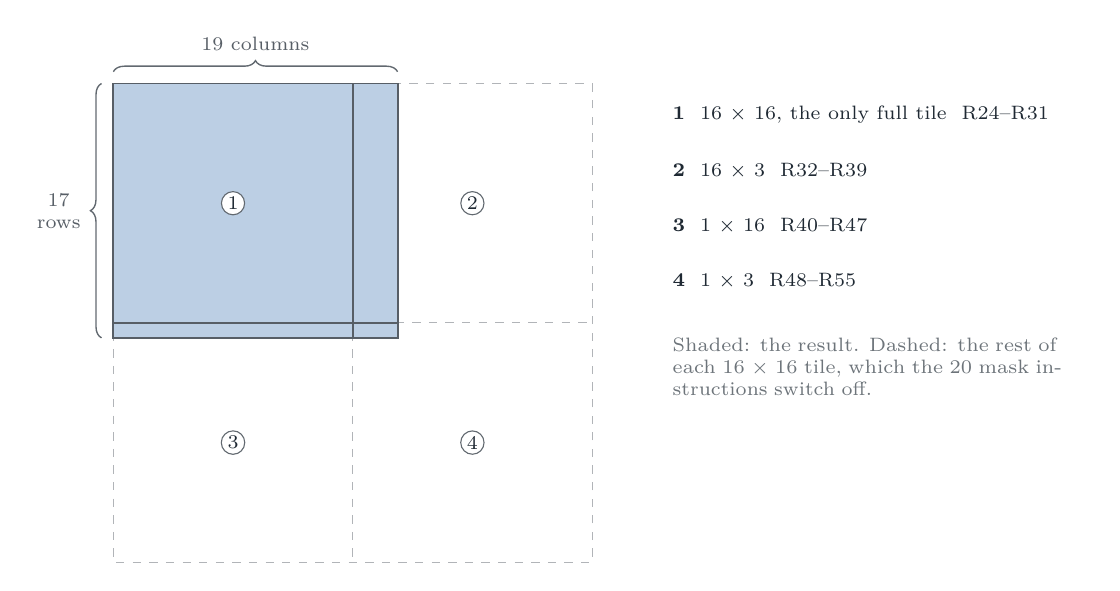
\begin{tikzpicture}[x=1mm, y=1mm,
    lbl/.style={tag, font=\scriptsize, align=center},
    num/.style={circle, draw=ink!70, fill=white, inner sep=0.8pt, font=\scriptsize, text=ink},
    key/.style={font=\scriptsize, text=ink, anchor=west}]

  \def\u{1.9}   % one element
  \def\g{60.8}  % 32 elements: the two tile rows and columns together

  % The part of the tile grid the matrix actually reaches.
  \fill[ours!30] (0,0) rectangle ({19*\u},{-17*\u});

  % The whole 32 x 32 tile grid, and the tile boundaries inside it.
  \draw[ink!35, line width=0.4pt, dashed] (0,0) rectangle ({\g},{-\g});
  \draw[ink!35, line width=0.4pt, dashed] ({16*\u},0) -- ({16*\u},{-\g});
  \draw[ink!35, line width=0.4pt, dashed] (0,{-16*\u}) -- ({\g},{-16*\u});

  % The live result on top of it.
  \draw[ink!75, line width=0.7pt] (0,0) rectangle ({19*\u},{-17*\u});
  \draw[ink!75, line width=0.7pt] ({16*\u},0) -- ({16*\u},{-17*\u});
  \draw[ink!75, line width=0.7pt] (0,{-16*\u}) -- ({19*\u},{-16*\u});

  \node[num] at ({8*\u},{-8*\u})  {1};
  \node[num] at ({24*\u},{-8*\u}) {2};
  \node[num] at ({8*\u},{-24*\u}) {3};
  \node[num] at ({24*\u},{-24*\u}){4};

  \draw[decorate, decoration={brace, amplitude=4pt}, line width=0.5pt, color=ink!70]
    (0,1.5) -- ({19*\u},1.5) node[midway, above=4pt, lbl] {19 columns};
  \draw[decorate, decoration={brace, amplitude=4pt, mirror}, line width=0.5pt, color=ink!70]
    (-1.5,0) -- (-1.5,{-17*\u}) node[midway, left=4pt, lbl] {17\\rows};

  % Key, clear of the drawing.
  \node[key] at ({\g+9},-4)  {\textbf{1}\ \ 16 × 16, the only full tile\ \ R24--R31};
  \node[key] at ({\g+9},-11) {\textbf{2}\ \ 16 × 3\ \ R32--R39};
  \node[key] at ({\g+9},-18) {\textbf{3}\ \ 1 × 16\ \ R40--R47};
  \node[key] at ({\g+9},-25) {\textbf{4}\ \ 1 × 3\ \ R48--R55};
  \node[key, text width=52mm, align=left, text=ink!65] at ({\g+9},-36)
    {Shaded: the result. Dashed: the rest of each 16 × 16 tile, which the 20 mask instructions
     switch off.};
\end{tikzpicture}
\caption{The running example's output against the tiles that cover it. A 17 × 19 result does not divide into
16 × 16, so it takes two tile rows by two tile columns, three of them partial: one \op{5107} and one
eight-register accumulator group each.}
\label{fig:example-tiles}
\end{figure}

 The compiler emits 101 instructions, grouped by phase in \cref{tab:example-phases}.

\begin{xltabular}{\linewidth}{@{}l>{\hsize=1.10\hsize}X>{\hsize=0.90\hsize}X@{}}
\caption{The example program's 101 instructions by phase, as read with Apple's decoder.}\label{tab:example-phases}\\
\toprule
Phase & Instructions & What they do \\
\midrule
\endfirsthead
\tablecontinued{3}
\toprule
Phase & Instructions & What they do \\
\midrule
\endhead
addresses & one \op{14060} reading the lane index, then
shifts, ANDs and adds & compute each lane's row, column and byte offset
(\cref{sec:fragment-layouts}) \\*
masks & 20 \op{612} and \op{437} & enable only the 17 rows and 19 columns that exist
(\cref{sec:masks-predicated-memory}) \\*
loads & 4 \op{12674} and 4 \op{12675} & gather two A and two B fragments, eight bytes per lane each \\*
multiply & 4 \op{5107} & one per output tile, since K = 16 is one slice \\*
stores & 2 \op{17257} and 6 \op{17258} & write the four tiles, masked where partial \\*
epilogue & \op{14059}, \op{12682}, \op{11842}, \op{998}, \op{17229}, \op{684} & add 1.0 to one element \\*
\bottomrule
\end{xltabular}

The first \op{5107} is the ten bytes \hash{a70405112204a4620202}, which Apple's decoder prints as:

\begin{lstlisting}
op5107  R24..R31 <- 0x01000000, 1, R20_R21_R22_R23, 0, 2, R68_R69_R70_R71, 0, 2
        D        operand 1         A fragment      lifetime, type   B fragment   lifetime, type
\end{lstlisting}

\begin{itemize}
\item \textbf{D, R24–R31,} is an eight-register fp32 accumulator group holding the output tile at application rows
  0–15, columns 0–15. The compiler packs every tile with the hardware's B lane map, so its labeling of these registers
  differs from the instruction's canonical one by a one-bit rotation of the row index. A is packed the same way, and
  the product is correct in application coordinates (\cref{sec:coordinate-systems}).
\item \textbf{A, R20–R23, and B, R68–R71,} are four-register fragments of 16-bit values. Type code 2 means half.
\item \textbf{Operand 1, 0x01000000,} is the destination's raw operand, which older notes call the flags word. Its
  bit 24 means wait for scoreboard slot 0. All eight tensor loads write slot 0. Each
  load's own control word, 0x01100000, both publishes slot 0 and waits on it (\cref{sec:scoreboard-publish-wait,sec:scoreboard}). On an MMA
  whose loads fill slot 7, clearing the matching wait bit made the multiply read its fragments before the loads landed,
  and it produced zeros (measured on a separate slot-7 program, MM~\mm{6}).
\item \textbf{The 1 that follows it} is constant; no encoding bit varies it (\cref{sec:field-maps}).
\end{itemize}

Each fragment is read by two of the four MMAs, and the second read releases it (\cref{tab:example-mma-releases}). Each output element sums 16
products in a fixed tree, adjacent pairs and then pairs eight apart, rounding to nearest-even fp32 at every step (the
rule fitted on half inputs, which this program uses). The program uses the from-zero form, with no C input, so the
sum starts from the first of the tree's four partial sums; the accumulating form adds C first
(\cref{sec:arithmetic-semantics-supported}).

The epilogue orders its late values through the scoreboard.

\begin{enumerate}
\def\labelenumi{\arabic{enumi}.}
\item The \op{14059} of the threadgroup position publishes slot 0.
\item The \op{12682} waits on slot 0 for its index register and publishes slot 7.
\item The \op{998} waits on slot 7 for the loaded value.
\item The store needs no wait: its value comes from an ALU instruction, and ALU results are interlocked (\cref{sec:dependences-issue-scalar}).
\end{enumerate}

Alongside the code, the compiler reports what an executor needs: the three bindings with their element types, which
binding is written, the 24 distinct (opcode, length) forms used, an empty constant pool, the register count and
the system registers read. The project's image-building code turns that into the object, metadata, library and archive Metal loads (\cref{ch:kernel-metadata-image}).

The program was then run on the GPU below Metal (measured; \code{docs/g17-first-dispatch-trials.md}, "A second authored tensor program
below Metal"). The native runtime wrote the program at allocation 0, offset 0x6c0. Relative to the first tensor
program it had run, the resource graph changed in nine fields: two view offsets, one C pointer, two binding pointers, the kernel
word at offset 0x3f8 (from 0xa to 0xc), and the A, B and C windows, which became 544, 608 and
1,292 bytes, exactly 17 × 16 halves, 16 × 19 halves and 17 × 19 floats.

Three fresh processes each submitted the program through IOGPU with no Metal loaded. In each, 323 of 323 fp32 outputs
were bit-exact, inputs and guards were intact, both completion callbacks arrived and no recovery event occurred. The
outputs hash to \hash{ec43027260f5a0b8dd59526c17102ffe00066852f10af42a91103c36e778faf6}, the same as an independently
computed reference and as the earlier run through Metal (\cref{ch:submission-below-metal}).

\section{Applications}\label{sec:understanding-supports}

InternLM2.5-1.8B decodes on the compiler's kernels, run through Metal. Single stream at a 1,024-token context, it runs
at 1.14× the decode rate of mlx-lm's \code{generate\_step}; the
\href{https://github.com/sbryngelson/AGXForge/blob/main/docs/demonstrations.md}{demonstrations document} gives the other models and
workloads with their baselines. MiniLM-L6 sentence retrieval and Qwen2.5-0.5B-Instruct generation ran through the native
submission path. Each stage was checked against a CPU recomputation from its GPU inputs, and each output against the
original checkpoint evaluated in FP64 (MM~\mm{25.210}; \cref{ch:below-metal-native}). The compiler
was also run on code it was not written for. Of the 125 sources that compiled from a fixed set of 197 (the census) when it
was run on the hardware, 101 have run and been checked, and none crashes the driver (MM~\mm{25.149.1}); today's front end
and backend compile 128 of the 197 (\cref{ch:source-native-program}).

A CPU emulator, working from the program bytes, executes one position of a shipped batched-decode graph and of
single-stream decode, dispatch by dispatch. All 316 and all 172 dispatches match the GPU byte for byte, as does a
16~MB prefill slice (MM~\mm{25.197}).

\section{Limits of the evidence}\label{sec:where-evidence-stops}

The InternLM2 decode lead over mlx-lm (\cref{sec:understanding-supports}) comes from the kernels. In a matched study,
Apple's compiler, given the same kernels, ran them 10–15 percent faster with identical tokens, so the lead does not show
that native instruction control is needed. The tensor-unit kernels were not part of that study (MM~\mm{25.211}).

Below Metal, MiniLM and Qwen run with checked results, but more slowly than Apple's paths: the matched MiniLM FFN and
attention blocks take 2.427 and 3.815~ms against Metal's 1.797 and 1.962~ms (MM~\mm{25.210.5}). One auxiliary control
in the native-path validation fails. Qwen's prefix logits, compared with an FP64 model that uses the same half-precision
projections, deviate by up to 0.097, and 10,658 elements fall outside the bound \code{0.025 + 0.002 * abs(reference)}
(\cref{ch:below-metal-native}).

Because validation uses Apple's decoder (\cref{sec:project-authors-two}), and the project's own decoder for its
programs was started and then paused, nothing here establishes portability (MM~\mm{25.209}).

\section{Conventions}\label{sec:read-this-document}

Rules and measurements in Part~\ref{part:i} carry one of these evidence tags, which say where a statement stands in
\cref{fig:evidence-flow}.

% Where the rules in this document come from, and what they constrain.
% (Mermaid 0.13 of the machine model, drawn properly.)
\begin{figure}[htbp]
\centering
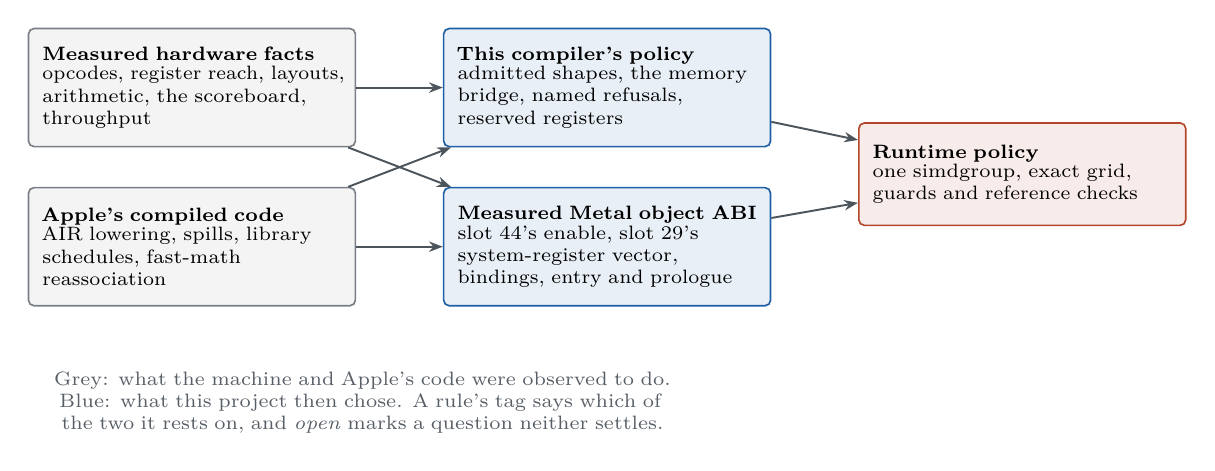
\begin{tikzpicture}[node distance=5mm and 11mm,
    src/.style={box, draw=ink!60, fill=ink!5, text width=38mm, align=left, font=\scriptsize,
      minimum height=15mm},
    pol/.style={box, draw=ours, fill=ours!10, text width=38mm, align=left, font=\scriptsize,
      minimum height=15mm},
    run/.style={box, draw=native, fill=native!10, text width=38mm, align=left, font=\scriptsize,
      minimum height=13mm}]

  \node[src] (hw)
    {\textbf{Measured hardware facts}\\[-1pt]opcodes, register reach, layouts, arithmetic, the
     scoreboard, throughput};
  \node[src, below=of hw] (ap)
    {\textbf{Apple's compiled code}\\[-1pt]AIR lowering, spills, library schedules, fast-math
     reassociation};

  \node[pol, right=of hw] (cc)
    {\textbf{This compiler's policy}\\[-1pt]admitted shapes, the memory bridge, named refusals,
     reserved registers};
  \node[pol, right=of ap] (abi)
    {\textbf{Measured Metal object ABI}\\[-1pt]slot 44's enable, slot 29's system-register
     vector, bindings, entry and prologue};

  \node[run, right=of cc, yshift=-11mm] (rt)
    {\textbf{Runtime policy}\\[-1pt]one simdgroup, exact grid, guards and reference checks};

  \draw[flow] (hw) -- (cc);
  \draw[flow] (ap) -- (cc);
  \draw[flow] (hw) -- (abi);
  \draw[flow] (ap) -- (abi);
  \draw[flow] (cc) -- (rt);
  \draw[flow] (abi) -- (rt);

  \node[tag, font=\scriptsize, anchor=north west, text width=82mm] at ([yshift=-7mm]ap.south west)
    {Grey: what the machine and Apple's code were observed to do. Blue: what this project then
     chose. A rule's tag says which of the two it rests on, and \emph{open} marks a question
     neither settles.};
\end{tikzpicture}
\caption{Where the rules in Part~\ref{part:i} come from. Measurement and observation of Apple's code constrain the
compiler's policy and the object ABI, and those two constrain what the runtime may do; the evidence tags above name
which kind of standing each rule has.}
\label{fig:evidence-flow}
\end{figure}


\begin{itemize}
\item \emph{measured}: run on this GPU and compared with an independent reference, with a control that could have failed;
\item \emph{measured (receipt fit)}: a recorded GPU output matched one candidate semantics among rivals; the replay checks
  consistency and is not independent evidence;
\item \emph{whole-program}: seen only inside programs verified bit-exact on the GPU, not run in isolation;
\item \emph{bounded negative}: searched for within a stated bound and not found; nothing is claimed beyond the bound;
\item \emph{Apple's compiler emits}: read from Apple's compiled code, which shows that a pattern works but leaves open
  whether the hardware requires it;
\item \emph{decoder}: what Apple's decoder prints or admits, with no execution behind it;
\item \emph{compile-witnessed}: a register number or form witnessed by compiling a source, with no dispatch confirming
  its values;
\item \emph{driver, static read}: read from the driver's code, not executed;
\item \emph{emulated}: run in the project's CPU emulator, which is checked against Apple's GPU;
\item \emph{this compiler}: a choice the project's compiler makes;
\item \emph{open}: unresolved.
\end{itemize}

Opcodes are named first and numbered second, as in "\op{12674}". The numbers are
Apple's opcode ids. The names are this project's, chosen by measured function, and are not Apple's spellings
(\cref{app:c}). Registers are written by hardware number (R0–R125), with their role stated where it matters.

Open questions are stated next to the rule they qualify and indexed in \cref{ch:not-known-index}. In Part~\ref{part:i}
a chapter with several open questions collects them in a paragraph headed \textbf{Not known}, and an \textbf{Evidence} list at the
end of a chapter, or of a long section, gathers the machine-model sections it cites.

\part{The machine}\label{part:i}
\chapter{Device and execution model}\label{ch:device-execution-model}

The measured part has 20 GPU cores. Each core issues from four SIMD slots, and the driver lets it hold up to 3,072
threads (\cref{sec:core-logical-resource,sec:residency-occupancy-rules}).

\leadhead{Notation.}

\begin{itemize}
\item \emph{Lane}: one thread's slot in a simdgroup. \emph{Simdgroup}: 32 lanes that issue one instruction stream together under an
  execution mask (\cref{ch:control-flow-execution}). \emph{Threadgroup}: one or more simdgroups that share threadgroup memory and can meet at a
  threadgroup barrier (\cref{sec:barriers-fences}). \emph{Grid}: all threadgroups of one dispatch.
\item \emph{Core}: one of the 20 GPU cores. Per-core figures divide a GPU-wide count by 20.
\item \emph{Resident}: a threadgroup (or simdgroup) is resident while it holds a core's resources, from launch until it ends.
  \emph{Residency} or \emph{occupancy}: how many are resident at once.
\item \emph{Registers used}: the highest 32-bit register named in the main program, plus one. \emph{Declared register count}: the value in
  per-kernel metadata slot 0 (\cref{sec:gpu-metadata-slots}).
\item \emph{Warm} and \emph{cold} refer to the GPU's performance state (\cref{sec:clocks-performance-states}).
\end{itemize}

\section{Measured platform and portability}\label{sec:measured-part-software}

All measurements were made on one Apple M5 Pro GPU (G17, the 20-core H17s), on the platform in
\cref{tab:measured-platform} (MM~\mm{22}, MM~\mm{25.66}, MM~\mm{25.91}). The below-Metal evidence
(\cref{ch:submission-below-metal}) records the OS build, 25G83. Most Metal-path evidence files record none, and for
those measurements the build in the table is the stated platform.
On 2026-10-02 the machine was updated to macOS 27.0.1 (build 26A434). Nothing in this reference was re-measured on that
build; the platform check described below reports the change, and the table gives the platform the figures were taken on.
The update renumbered Apple's decoder; the tools translate back to the numbering used here (\cref{sec:decoder-renumbering}).

\begin{xltabular}{\linewidth}{@{}>{\hsize=0.65\hsize}X>{\hsize=1.40\hsize}XX@{}}
\caption{The measured platform.}\label{tab:measured-platform}\\
\toprule
Component & Value & How read \\
\midrule
\endfirsthead
\tablecontinued{3}
\toprule
Component & Value & How read \\
\midrule
\endhead
Machine & \code{Mac17,8}, Apple M5 Pro & \code{sysctl hw.model} \\*
GPU & "Apple M5 Pro", 20 cores, Metal 4; Apple's internal
names H17s, \code{applegpu\_g17s} & \code{system\_profiler}; the core count is the
project's record (below) \\*
macOS & 26.6.2, build 25G83; Darwin 25.6.0 & \code{sw\_vers}, \code{uname} \\*
GPU user driver & \code{AGXMetalG17X.bundle} 353.14 & MM~\mm{25.141.20} \\*
Metal compiler & metal 32023.921 (metalfe-32023.921.6), target air64-apple-darwin25.6.0,
against an OS-side GPU compiler at 32023.886 & \code{xcrun metal --version}; MM~\mm{22} \\*
Xcode / SDK & Xcode 27.0 (27A266a), macOS SDK 27.0 & \code{xcodebuild -version} \\*
Host compiler & Apple clang 21.0.0 (clang-2100.3.34.2) & \code{clang --version} \\*
Apple's AGX3 decoder & inside
\code{GPUCompiler.framework/Versions/32023/Libraries/libLLVM.dylib} & \cref{sec:decoder} \\*
\bottomrule
\end{xltabular}

\code{sysctl -n hw.ncpu} returns 18, the CPU core count, which the project has mistaken for the GPU core count before. The GPU core count is not
readable through sysctl and is carried as the project's record; a platform pin that confused the two would put a
wrong divisor under every per-core figure (MM~\mm{25.66}). \code{tools/g17platform.py --check} compares the running machine with
this record and names each field that differs.

Nothing here is claimed for another part, OS build or compiler. Another G17 product may have a different core count, a
different populated register file and other loader variants, and no row of the project's ledger claims a result for
one (MM~\mm{0.1}, MM~\mm{25.66} row T9, MM~\mm{25.119}). MM~\mm{25.119} ranks results by how likely they are to change:

\begin{itemize}
\item \emph{Properties of the toolchain}, which follow Apple's compiler rather than the silicon and are the likeliest to move:
  which source forms reach the tensor unit, metadata layout classes, the constant-program laws, which opcodes Apple's
  compiler selects, spill counts.
\item \emph{Properties of the core count and clock} (residency counts, speeds, power), which change whenever either
  does.
\item \emph{Encodings and arithmetic}, the least likely to move within this generation: field maps, the register namespace,
  the tensor unit's reduction arithmetic.
\end{itemize}

Several conventions are conserved from Apple's earlier G13 generation and its public reconstruction in Mesa: the
length-bit cluster in the encoding (\cref{sec:framing}) and the command-stream layout below Metal, which decodes field for
field against Mesa's G13 description (\cref{ch:submission-below-metal}). Mesa's model was used only to suggest hypotheses and is not evidence for G17.

Apple's decoder admits the same ten tensor MMA opcodes when told the CPU is g17s, g17g or g18, and decodes the same
bytes as unrelated instructions for g17, g16 and g15 targets, so the admission is a property of the decoder tables
(MM~\mm{2}; \cref{sec:admission-decodes-executes}). The byte-identity pins, static checks and the metadata determinant over
the committed corpus run on the CPU without a GPU (MM~\mm{25.119}); those that decode programs need Apple's decoder, and
so macOS (\cref{sec:project-authors-two}).

\section{Threads, simdgroups, threadgroups and grids}\label{sec:threads-simdgroups-threadgroups}

SIMD width is 32 (measured; \code{threadExecutionWidth} is the driver constant 32 for every pipeline, MM~\mm{25.141.20},
MM~\mm{25.147}); \cref{fig:execution-hierarchy} is the hierarchy above it.

% Grid, threadgroup, simdgroup and lane: what each level owns and what it shares.
\begin{figure}[htbp]
\centering
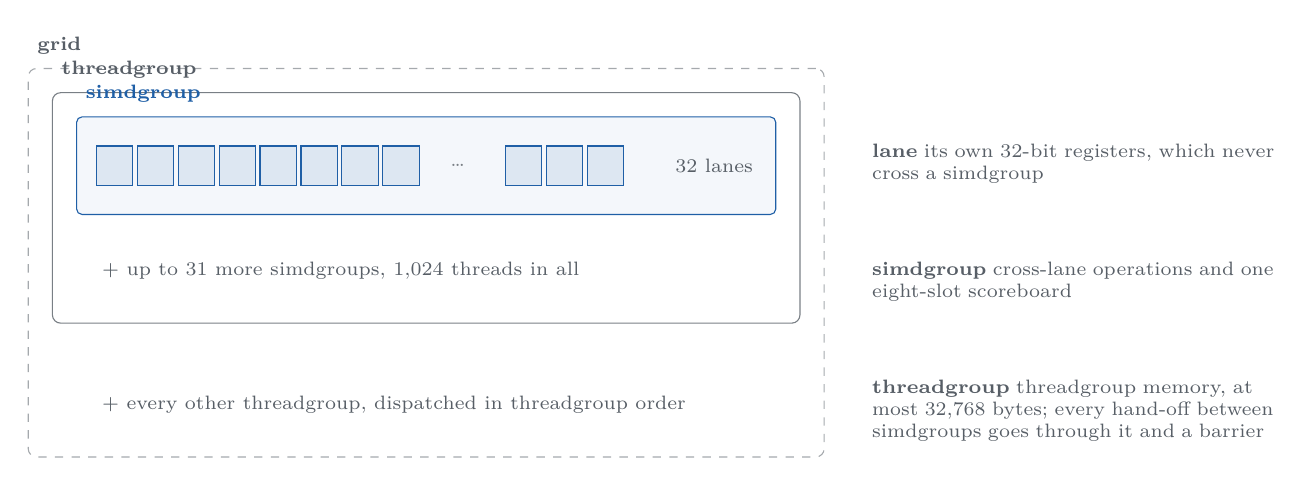
\begin{tikzpicture}[x=1mm, y=1mm,
    lane/.style={draw=ours, fill=ours!15, line width=0.4pt, minimum width=4.6mm,
      minimum height=5mm, inner sep=0pt, font=\tiny},
    lvl/.style={tag, font=\scriptsize, align=left, anchor=north west, text width=51mm}]

  % One simdgroup: 32 lanes, drawn as eleven with an ellipsis.
  \foreach \i in {0,...,7} \node[lane] at ({\i*5.2},0) {};
  \node[font=\scriptsize, text=ink!60] at (43.6,0) {\dots};
  \foreach \i in {10,...,12} \node[lane] at ({\i*5.2},0) {};
  \node[tag, font=\scriptsize, anchor=west] at (70,0) {32 lanes};

  \coordinate (sgA) at (-2.8,-4.2);
  \coordinate (sgB) at (82,4.2);
  \begin{scope}[on background layer]
    \node[draw=ours, rounded corners=2pt, fill=ours!5, inner sep=2mm, fit=(sgA) (sgB)] (sg) {};
  \end{scope}
  \node[tag, font=\scriptsize\bfseries, anchor=south west, text=ours]
    at ([yshift=0.5mm]sg.north west) {simdgroup};

  % The threadgroup holds up to 32 of them.
  \node[tag, font=\scriptsize, anchor=north west] at (-2.8,-11)
    {+ up to 31 more simdgroups, 1,024 threads in all};
  \coordinate (tgA) at (-2.8,-17);
  \begin{scope}[on background layer]
    \node[draw=ink!60, rounded corners=3pt, inner sep=3mm, fit=(sg) (tgA)] (tg) {};
  \end{scope}
  \node[tag, font=\scriptsize\bfseries, anchor=south west]
    at ([yshift=0.5mm]tg.north west) {threadgroup};

  \node[tag, font=\scriptsize, anchor=north west] at (-2.8,-28)
    {+ every other threadgroup, dispatched in threadgroup order};
  \coordinate (grA) at (-2.8,-34);
  \begin{scope}[on background layer]
    \node[draw=ink!40, dashed, rounded corners=3pt, inner sep=3mm, fit=(tg) (grA)] (grid) {};
  \end{scope}
  \node[tag, font=\scriptsize\bfseries, anchor=south west]
    at ([yshift=0.5mm]grid.north west) {grid};

  % What each level owns.
  \node[lvl] at (95,4) {\textbf{lane} its own 32-bit registers, which never cross a
    simdgroup};
  \node[lvl] at (95,-11) {\textbf{simdgroup} cross-lane operations and one eight-slot
    scoreboard};
  \node[lvl] at (95,-26) {\textbf{threadgroup} threadgroup memory, at most 32,768 bytes;
    every hand-off between simdgroups goes through it and a barrier};
\end{tikzpicture}
\caption{The execution hierarchy. SIMD width is 32 on every pipeline measured, and a threadgroup holds at most
1,024 threads.}
\label{fig:execution-hierarchy}
\end{figure}

 A tensor fragment is a per-lane register tuple across those 32 lanes (\cref{ch:tensor-unit}).

\begin{itemize}
\item A threadgroup holds at most 1,024 threads. \code{maxTotalThreadsPerThreadgroup} is a field of the compiler's reply that
  the driver copies; 0 or absent becomes 1,024 (driver, static read, MM~\mm{25.141.20}). It read 1,024 for every pipeline
  tested, from 4 to 512 live scalars per thread and 64 to 32,768 bytes of threadgroup memory (measured, MM~\mm{25.47}), so it
  does not vary with register use.
\item Registers are per lane and never cross simdgroups. Every hand-off between simdgroups goes through memory and a
  barrier (\cref{sec:barriers-fences}); cross-lane movement inside a simdgroup is covered in \cref{ch:cross-lane-operations}.
\item Apple's GPU compiler on this toolchain refuses more than 32,768 bytes of threadgroup memory per threadgroup (48, 60
  and 64 KiB refused; 96 KiB drops the compiler connection; MM~\mm{7}, MM~\mm{0.1}). Metal's pipeline creation does not check the
  declared size: a container declaring 1 MiB builds and reports 1,048,576 back (MM~\mm{25.147}; \cref{sec:object-library-archive}).
\item Position registers (lane index, simdgroup index, threadgroup and grid positions) are special registers read by
  instruction; \cref{ch:special-registers} lists them.
\item Grids are dispatched in threadgroup order, and the driver prepares fast-division constants to split a linear
  threadgroup index into three dimensions (MM~\mm{25.141.20}; what this means for forward progress is in \cref{sec:forward-progress-in-order}).
\end{itemize}

\section{Core resource model}\label{sec:core-logical-resource}

% One core's logical resources: what runs beside what, and what contends.
\begin{figure}[htbp]
\centering
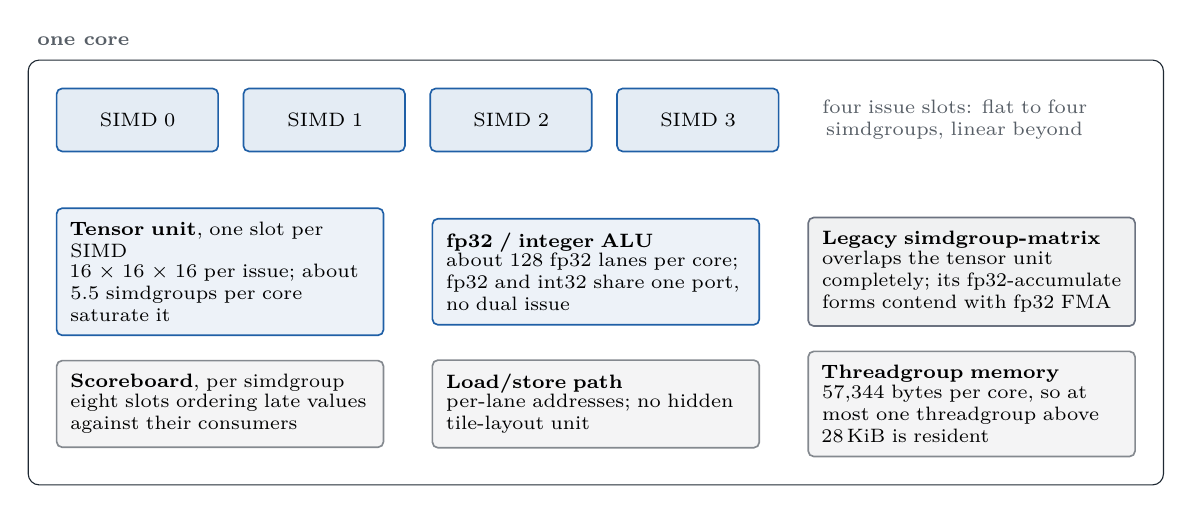
\begin{tikzpicture}[node distance=3mm and 6mm,
    unit/.style={box, text width=38mm, align=left, font=\scriptsize, minimum height=10mm},
    sl/.style={box, draw=ours, fill=ours!12, text width=17mm, align=center,
      font=\scriptsize, minimum height=8mm}]

  \node[sl] (s0) {SIMD 0};
  \node[sl, right=3mm of s0] (s1) {SIMD 1};
  \node[sl, right=3mm of s1] (s2) {SIMD 2};
  \node[sl, right=3mm of s2] (s3) {SIMD 3};
  \node[tag, font=\scriptsize, anchor=west, text width=34mm] at ([xshift=4mm]s3.east)
    {four issue slots: flat to four simdgroups, linear beyond};

  \node[unit, below=7mm of s0.south west, anchor=north west, draw=ours, fill=ours!8]
    (tu) {\textbf{Tensor unit}, one slot per SIMD\\[-1pt]16 × 16 × 16 per issue; about 5.5
      simdgroups per core saturate it};
  \node[unit, right=of tu, draw=ours, fill=ours!8]
    (alu) {\textbf{fp32 / integer ALU}\\[-1pt]about 128 fp32 lanes per core; fp32 and int32
      share one port, no dual issue};
  \node[unit, right=of alu, draw=apple, fill=apple!10]
    (leg) {\textbf{Legacy simdgroup-matrix}\\[-1pt]overlaps the tensor unit completely;
      its fp32-accumulate forms contend with fp32 FMA};

  \node[unit, below=of tu, draw=ink!55, fill=ink!5]
    (sb) {\textbf{Scoreboard}, per simdgroup\\[-1pt]eight slots ordering late values against
      their consumers};
  \node[unit, right=of sb, draw=ink!55, fill=ink!5]
    (ls) {\textbf{Load/store path}\\[-1pt]per-lane addresses; no hidden tile-layout unit};
  \node[unit, right=of ls, draw=ink!55, fill=ink!5]
    (tgm) {\textbf{Threadgroup memory}\\[-1pt]57,344 bytes per core, so at most one
      threadgroup above 28\,KiB is resident};

  \begin{scope}[on background layer]
    \node[draw=ink, rounded corners=4pt, inner sep=3.5mm, fit=(s0) (s3) (tu) (tgm)] (core) {};
  \end{scope}
  \node[tag, font=\scriptsize\bfseries, anchor=south west] at ([yshift=0.5mm]core.north west)
    {one core};
\end{tikzpicture}
\caption{One core, as measured concurrency describes it: which streams run beside each other and which contend.
This is a logical account and does not locate or count physical units (\cref{tab:core-resources}).}
\label{fig:core-resources}
\end{figure}


The model in \cref{tab:core-resources} and \cref{fig:core-resources} is a \emph{logical} account of measured concurrency: which streams run side by side without slowing each
other, and which contend. It does not locate or count physical units (MM~\mm{0.2}).

\begin{xltabular}{\linewidth}{@{}>{\hsize=0.65\hsize}X>{\hsize=1.59\hsize}X>{\hsize=0.75\hsize}X@{}}
\caption{Logical resources of one core.}\label{tab:core-resources}\\
\toprule
Resource & Measured behavior & Source \\
\midrule
\endfirsthead
\tablecontinued{3}
\toprule
Resource & Measured behavior & Source \\
\midrule
\endhead
Four SIMD issue slots per core & One, two or four simdgroups each running a dependent tensor MMA chain
take 32.8, 32.4 and 32.8~µs; eight take 57.5, sixteen 112.6, thirty-two
224.3: flat to four, linear beyond & measured, MM~\mm{8} \\*
Tensor unit, one slot per SIMD & 16 × 16 × 16 per issue, 1,024 flop per cycle per core at saturation;
about 5.5 simdgroups per core saturate it & measured, MM~\mm{8}; \cref{ch:tensor-unit} \\*
fp32 / integer ALU & about 4.1 × $10^{12}$ fp32 adds per second machine-wide, consistent with
128 fp32 lanes per core at about 1.6~GHz; no dual issue between
fp32 and int32 (ffma + iadd mixed 3.61~ns per op against 3.64 predicted
for one shared port and 2.09 for dual issue) & measured, MM~\mm{0.15} \\*
Legacy simdgroup-matrix engine & overlaps the tensor unit completely at 16 and 32 simdgroups per core;
its fp32-accumulate forms contend with fp32 FMA (overlap 0.37 or less),
its half-accumulate form mostly does not (0.66–0.95) & measured, MM~\mm{9}; \cref{sec:legacy-simdgroup-matrix-engine} \\*
Per-simdgroup scoreboard & eight slots ordering late values (loads, special-register reads,
atomics) against their consumers & measured, MM~\mm{6}; \cref{sec:scoreboard} \\*
Load/store path & per-lane addresses; no hidden tile-layout unit & measured, MM~\mm{23.2}; \cref{ch:memory} \\*
\bottomrule
\end{xltabular}

\section{Residency and occupancy rules}\label{sec:residency-occupancy-rules}

The measured counts, the per-core staircase and the cost of registers and spills behind them are in
\cref{sec:registers-spills-occupancy,sec:residency-occupancy-measurements}.

\begin{enumerate}
\def\labelenumi{\arabic{enumi}.}
\item Residency follows the registers a program uses, not the count it declares (measured, MM~\mm{25.115}). The same bytes
  declaring 19 and declaring 125 reach the same peak every time (1,814–1,896 resident at 2,048 launched simdgroups); only
  using more registers lowers the peak. The declared count (metadata slot 0) is inert for residency between 19 and
  125, and inert for execution: code using R0–R123 runs correctly declaring 124, 127, 128, 160 or 224 (MM~\mm{10}).
  Below Metal the count travels to the hardware in a launch-state packet (\cref{sec:gpu-metadata-slots}, \cref{ch:submission-below-metal}); whether that
  packet's value affects residency was not isolated.
\item The driver caps threadgroups per core at \code{min(3072 / threads\_per\_threadgroup, 96)} (driver, static read,
  MM~\mm{25.141.20}): 3,072 threads per core, 96 simdgroups of 32. Nothing in that path reads the register count; any
  register-dependent limit lies below the driver or in the compiler's reply. The measured peak at 19 registers,
  95.0 simdgroups per core (MM~\mm{25.121}), equals this cap.
\item Register pressure lowers residency, by a kernel-dependent amount. Two probes disagree by about a factor of two
  at high register counts (about 64 against about 32 simdgroups per core near 125 registers; the counts and their
  kernels are given in \cref{sec:residency-occupancy-measurements}), and which kernel property the difference follows is
  open (MM~\mm{25.121}).
\item The per-core threadgroup-memory budget is 57,344 bytes (56 KiB) (measured, MM~\mm{25.49}): two threadgroups of
  28,672 bytes fit on a core, one of 28,688 does, and the 16-byte step costs 25 percent in run time. With the 32 KiB per-threadgroup
  limit, at most one threadgroup above 28 KiB is resident per core.
\item For 1,024-thread threadgroups, no residency count may be assumed. The forward-progress probe ran 200 threadgroups of
  1,024 threads, one producer last, with no consumer starving (17–21~µs); had fewer than 200 been co-resident, the
  earliest consumers would have spun to the 200,000-poll cap before the last-dispatched producer ran (MM~\mm{25.141.1}).
  That implies at least 10 per core. The driver formula gives 3 per core (60 GPU-wide) (MM~\mm{25.141.20}). The two numbers
  have not been reconciled, and the 800-threadgroup row (480 of 799 at the cap) does not give a simultaneous count,
  because waves can reach the cap one after another.
\end{enumerate}

\textbf{Not known.} Neither the physical register capacity per core nor its allocation granularity is known. Residency is not one fixed
pool divided by per-simdgroup demand (a fixed-pool model under-predicts the measured count about fourfold at 126
registers; \cref{sec:residency-occupancy-measurements}, MM~\mm{24.2} row H4, MM~\mm{25.49}), and whether that means a larger file than any published part or
registers that are not all physically resident is not separable with these instruments (MM~\mm{25.20}). Metal's public API
has no occupancy counter on this part (MM~\mm{25.48}; \cref{sec:dispatch-encoder-command-buffer}).

\section{Forward progress}\label{sec:forward-progress-in-order}

All results in this section come from one probe family, each probe one dispatch (\code{tools/g17gpuprobes/fp.m}): consumers spin, capped at 200,000 polls, until an atomic count
reaches the number of producers placed at the end of the grid (MM~\mm{25.141.1}; \cref{tab:forward-progress-probe}).

\begin{xltabular}{\linewidth}{@{}XlX@{}}
\caption{Forward-progress probe results by grid shape (MM~\mm{25.141.1}).}\label{tab:forward-progress-probe}\\
\toprule
Grid (threadgroups × threads) & Producers & Consumers at the cap \\
\midrule
\endfirsthead
\tablecontinued{3}
\toprule
Grid (threadgroups × threads) & Producers & Consumers at the cap \\
\midrule
\endhead
64 to 1,200 × 32 & 1, the last & 0 (none waited more than 94 polls) \\*
2,000 × 32 & 1 & 1,688 of 1,999 \\*
20,000 × 32 & 1 & 18,350 of 19,999 \\*
20 to 200 × 1,024 & 1 & 0 \\*
800 × 1,024 & 1 & 480 of 799 \\*
\bottomrule
\end{xltabular}

\begin{itemize}
\item Among resident threadgroups, no starvation was observed. Up to 1,200 single-simdgroup threadgroups and up to 200
  of 1,024 threads, every consumer saw its producer within the cap (at most 94 polls in the 32-thread rows).
\item With 2,000 threadgroups the first resident wave (about 1,690, about 84 per core at
  that register count) spun to its cap before the producer, dispatched last, ran, and the threadgroups that
  succeeded were the high-numbered ones. That fits in-order dispatch of threadgroups with no preemption of a
  spinning one (MM~\mm{25.141.1}).
\item In the persistent-kernel runs (16 phases, totals exact), grid barriers among resident threadgroups all completed
  without reaching the cap, and a barrier cost more than a dispatch boundary at every measured shape (MM~\mm{25.141.1};
  costs in \cref{ch:performance}).
\end{itemize}

Code may not assume any of the following:

\begin{itemize}
\item that a threadgroup waiting on another threadgroup will see it run, unless both are resident; a spin-wait on a
  producer that is not resident may wait indefinitely, and nothing measured shows preemption letting the producer run
  (MM~\mm{25.141.1}; MM~\mm{17} rule 40, MM~\mm{0.15});
\item that "in order" means anything finer than dispatch order of threadgroups. Completion order and memory ordering between threadgroups
  are covered in \cref{sec:ordering-across-lanes} (visibility needs a device fence on both
  sides; ordering comes from an atomic);
\item that a timeout protects the machine. Killing the host process does not cancel a kernel: an unbounded loop kept the GPU
  at 100 percent with nothing dispatching until a reboot (MM~\mm{25.116}), and an unbounded data-driven trip count once
  rebooted the machine (MM~\mm{25.90}). Loops in this project's compiler are capped so that termination is provable
  (\cref{sec:loops-loop-variable-rule}, \cref{ch:control-flow-execution}).
\end{itemize}

A persistent kernel should size its grid to the resident capacity measured for its own register and
threadgroup-memory use, and pull work from an atomic queue; any other hand-off between
threadgroups goes through a dispatch boundary (MM~\mm{17} rule 40).

\section{Clocks}\label{sec:clocks-performance-states}

The top clock is about 1.62~GHz: 1,620~MHz read from \code{powermetrics} at 100 percent residency in the top bin;
1.63~GHz is implied by the saturated tensor issue rate of 32 cycles per MMA (measured, MM~\mm{8}, MM~\mm{20};
\cref{sec:clocks-power-gpu}).

\begin{itemize}
\item A run shorter than about 1.5~ms runs at whatever frequency the GPU is
  idling at, and a longer one speeds up partway (MM~\mm{25.121}); a cold GPU ran the same kernel about 4 to 4.8 times slower
  than after sustained load (MM~\mm{22}, MM~\mm{25.115}). Timings need a saturating warm-up in the same process (the project uses
  4,096 threadgroups of 256) and a reference dispatch to detect a clock change.
\item The governor reacts to command-buffer shape. Metal System Trace records the GPU performance state (Minimum,
  Medium, Maximum) per interval; a workload issuing seven short command buffers per step spent 27–78 percent of its time
  in Medium, while one long command buffer per step stayed at Maximum (two recordings, direction reproduced, size not;
  MM~\mm{0.15}).
\item In-run variation was 0.4–1.3 percent, but the same configuration in two
  processes differed by 9–13 percent; compare arms interleaved in one process (MM~\mm{16}, MM~\mm{25.126}; further figures at the start of \cref{ch:performance}).
\item Several results published earlier in the project were artifacts of the idle clock (a
  residency "shortfall", a "bimodal" issue rate); each is corrected where it is used (MM~\mm{25.115}, MM~\mm{25.122}).
\end{itemize}

\textbf{Evidence.} MM~\mm{0.1}, MM~\mm{0.2}, MM~\mm{0.15}, MM~\mm{2}, MM~\mm{7}, MM~\mm{8}, MM~\mm{9}, MM~\mm{10}, MM~\mm{16},
MM~\mm{17} (rule 40), MM~\mm{20}, MM~\mm{22}, MM~\mm{24.2} (row H4), MM~\mm{25.20}, MM~\mm{25.47}, MM~\mm{25.48},
MM~\mm{25.49}, MM~\mm{25.66}, MM~\mm{25.90}, MM~\mm{25.91}, MM~\mm{25.115}, MM~\mm{25.116}, MM~\mm{25.119},
MM~\mm{25.121}, MM~\mm{25.122}, MM~\mm{25.126}, MM~\mm{25.141.1}, MM~\mm{25.141.20}, MM~\mm{25.147}.

\chapter{The register file}\label{ch:register-file}

Each lane of a simdgroup owns a private file of 32-bit general registers, addressed by number in the instruction and
also viewed as 16-bit halves and as 2-, 4- and 8-register tuples. Beside it sits a uniform file, written once per
dispatch. No register renaming is visible to software. Each register source carries a \emph{modifier} that can
negate, take the absolute value of, or \emph{release} the value; some forms do not let the compiler choose it
(\cref{tab:fixed-modifiers}).

Fields can name R0–R143, but the hardware executes only R0–R125 (\cref{sec:namespace,fig:register-file}). Some fields are narrower than
the namespace: certain forms can name only R0–R15, and others cannot name particular registers at all
(\cref{sec:narrow-fields-narrow,sec:encoding-holes}). Register choice has to satisfy each form's constraints, which a
graph coloring over one homogeneous register file does not capture. Lifetime is encoded in the instruction and applies
per lane, under the execution mask. The last reader of a value marks it released, and no hardware mechanism notices a
later read (\crefrange{sec:operand-modifiers}{sec:loops-loop-variable-rule}). When kernels are composed, a value
live across a region boundary, such as a loop header, a fused stage or a second GEMM, must not be released before that
boundary in the emitted code.

% The register namespace: what the fields can name against what the hardware runs,
% and the files beside the general one.
\begin{figure}[htbp]
\centering
\begin{tikzpicture}[y=1mm, x=1mm,
    seg/.style={draw, line width=0.6pt, align=center, font=\scriptsize, minimum height=8mm},
    lbl/.style={tag, font=\scriptsize, align=center},
    side/.style={box, text width=34mm, align=left, font=\scriptsize}]

  % The GPR32 namespace as one bar: 144 names, 126 of them executable.
  \node[seg, draw=ours, fill=ours!12, minimum width=88mm, anchor=west] at (0,0)
    (run) {R0--R125\\[-2pt]{\scriptsize execute}};
  \node[seg, draw=apple, fill=apple!14, minimum width=14mm, anchor=west] at (88,0)
    (pair) {R126\\[-2pt]R127};
  \node[seg, draw=ink!45, fill=ink!6, minimum width=30mm, anchor=west] at (102,0)
    (ext) {R128--R143};

  \node[lbl, above=1.5mm of run] {126 registers the allocator may use};

  % Staggered so the two annotations cannot overprint, each on its own leader.
  \node[lbl, text width=26mm, anchor=north] at (95,-8) (pairl) {named, not populated};
  \draw[ink!45, line width=0.4pt] (95,-4) -- (95,-7.6);
  \node[lbl, text width=38mm, anchor=north] at (117,-17) (extl)
    {decoder-visible names; every instruction squashed};
  \draw[ink!45, line width=0.4pt] (117,-4) -- (117,-6) -- (117,-16.6);

  \draw[decorate, decoration={brace, amplitude=4pt, mirror}, line width=0.6pt, color=ink!70]
    (0,-27) -- (132,-27)
    node[midway, below=5pt, lbl] {GPR32: 144 names the operand fields can express};

  % The same storage under three other views.
  \node[side, anchor=north west, draw=ours, fill=ours!8] at (0,-38)
    (halves) {\textbf{halves} GPR16, 288 members\\R0L, R0H, \dots, R143H; a field counting
      halves names 2n + h. A 16-bit write leaves the other half alone.};
  \node[side, anchor=north west, draw=ours, fill=ours!8] at (49,-38)
    (tuples) {\textbf{tuples} tup2, tup4, 143 / 141 members; tup8\_alignedrc, the eighteen
      8-aligned groups. A base must be naturally aligned, never rounded.};
  \node[side, anchor=north west, draw=ours, fill=ours!8] at (98,-38)
    (tensor) {\textbf{tensor operands} classes 41, 159 and 335: 2-, 4- and 8-register tuples,
      found nowhere else in the table.};

  % The files that sit beside it.
  \node[side, anchor=north west, draw=apple, fill=apple!12] at (0,-64)
    (uni) {\textbf{uniform file} u0, u1, \dots, written once per dispatch by the constant
      program; in MMA programs u0--u5 are reserved.};
  \node[side, anchor=north west, draw=apple, fill=apple!12] at (49,-64)
    (ir) {\textbf{IR32} IR0--IR15. \code{IRGPR32} admits them beside R0--R143, but all 229
      corpus writes land in ordinary registers.};
  \node[side, anchor=north west, draw=apple, fill=apple!12] at (98,-64)
    (flag) {\textbf{FLAGR} FLAG0--FLAG14 plus FLAGTRUE and FLAGFALSE; compact forms reach
      FLAG0--FLAG6 only.};
\end{tikzpicture}
\caption{The register namespace. The operand fields can express 144 general-register names; the measured part
runs 126 of them. Below, the same storage under its other views, and the files that sit beside it.}
\label{fig:register-file}
\end{figure}


\leadhead{Notation.}

\begin{itemize}
\item \emph{Rn}: general register n, 32 bits per lane. \emph{RnL}, \emph{RnH}: its low and high 16-bit halves. \emph{Ra\_\dots{}\_Rb}: a tuple
  (for example R20\_R21\_R22\_R23, a 16-bit tensor fragment).
\item \emph{MCRegister id}: the number Apple's decoder uses for a register; the general block starts at 105, so Rn has id
  105 + n (verified over 300 registers in 60 shaders; \code{docs/agx3-oracle.md} section 6). The project's code writes
  "r119" for id 119, which is R14; this chapter always writes hardware numbers.
\item \emph{Slot domain}: an operand field value counting halves, 2 × n + h (h = 0 low, 1 high) (decoder, MM~\mm{25.139.1}).
\item \emph{Modifier}: the immediate operand that follows a register source (\cref{sec:operand-modifiers}). \emph{Release} (weight 16), \emph{keep}
  (weight 32).
\item \emph{Late value}: a result that arrives after its producer issues and needs a scoreboard wait (\cref{sec:scoreboard}).
\item \emph{Registers used} (\cref{ch:device-execution-model}) equals the declared count this compiler writes into
  metadata slot 0 (\cref{sec:gpu-metadata-slots}).
\end{itemize}

\begin{xltabular}{\linewidth}{@{}XX@{}}
\caption{Register-file rules and their evidence.}\label{tab:register-statements}\\
\toprule
Statement & Standing \\
\midrule
\endfirsthead
\tablecontinued{2}
\toprule
Statement & Standing \\
\midrule
\endhead
R0–R125 execute; naming R126–R143 squashes the whole instruction & measured (MM~\mm{10}, MM~\mm{25.18}) \\*
After a release no controlled probe read the old value; the release acts per lane, gated by
the execution mask & measured (MM~\mm{6}, MM~\mm{25.95}) \\*
A released register's later read returns 0 & observed in every controlled run; not established as a rule
(\cref{sec:release-does}) \\*
Loop-carried values must not be released before the back edge & measured, with a machine-hanging failure (MM~\mm{25.116}) \\*
8N + K ≤ 115 and 8N + 4M ≤ 108 & measured frontiers of the kernels tested (MM~\mm{11}) \\*
Field widths and holes & decoder (Apple's decoder reading back the
encoder's bytes) \\*
\bottomrule
\end{xltabular}

\section{Register namespace}\label{sec:namespace}

Allocate only R0–R125: 126 registers per lane, fifteen eight-register groups at bases R0, R8, \dots{}, R112
(measured, MM~\mm{10}, MM~\mm{0.7}). Any instruction that names R126, R127 or R128–R143 in \emph{any} register operand is squashed as a
whole: no register write, no memory write, no atomic, no tensor-unit time, and no error from the compiler, the driver
or the API (measured, MM~\mm{17} rule 1).

The boundary first showed up as a store of a tuple reaching R126 that failed to round-trip, independent of the
declared count. A follow-up wrote through R126 and R127, read zeros from the output buffer, and was recorded as
R126 and R127 \emph{reading as zero and dropping writes}, like a hardwired zero register. For an instruction that reads
R126 and stores it, such a register stores 0, while a discarded instruction stores nothing. The output buffer had been
zero-filled before the dispatch, so the two leave the same bytes. With the buffer filled with a sentinel instead, the
sentinel survived, so the store had not executed (MM~\mm{19}, MM~\mm{25.20}). The first check of a later loop kernel,
the wide RMSNorm (\cref{sec:release-does}), had the same flaw, since its output carried no sentinel.
The same test was then repeated in every operand role: ALU sources and destinations, store sources of three widths, a
store's index register, a load's destination group, an atomic's destination, and the tensor MMA's accumulator, A and B
operands (MM~\mm{10}). In each the whole instruction is discarded, including the parts that do not touch the high register. For R128–R143 the result
is unchanged by declared register counts from 12 to 255, by one against 32 simdgroups, and by a 32- against a
1,024-thread pipeline limit (MM~\mm{25.18}).

\code{agxforge/g17/registerdomain.py} encodes the rule: \code{ALLOCATABLE\_MAX = 125}, \code{REGISTER\_COUNT = 126},
\code{MAX\_FP32\_ACCUMULATOR\_GROUPS = 15}, group starts on a multiple of 8 (this compiler). Whether another G17 implementation backs the higher names with storage is not tested (MM~\mm{25.18}).

\begin{itemize}
\item \emph{R126 and R127} are the top pair of a 128-register architectural file that this part populates only to R125. Three
  routes agree on 128: the half-register move's seven-bit source field plus a one-bit file selector (128 halves × 2
  files = 256 halves = 128 registers, measured in this repository); the five-bit accumulator selector's eighteen groups, of which
  exactly fifteen lie inside R0–R125, one straddles (R120–R127) and two lie wholly beyond; and, as a hypothesis source
  only, Mesa's G13 model of 256 sixteen-bit slots. Sentinel stores rule out a hardwired zero and unique encodings rule
  out aliases, and no metadata or launch control enables the two registers (MM~\mm{24.2} row H1, MM~\mm{25.20}). Whether anything \emph{reserves} the
  top pair, or the part simply populates 126 of 128, is open; the measurements here cannot separate the two.
\item \emph{R128–R143} are decoder-visible names outside that file, reachable only through fields wide enough to express them
  (accumulator-selector groups 16 and 17, nine-bit slot fields). Load and store register fields reach R127 only, so for
  those forms R126/R127 are expressible and R128–R143 are not (MM~\mm{24.2} row H1, MM~\mm{25.38}). The larger uniform file
  that G13 and Mesa expose is selected by operand type, so it does not explain them (MM~\mm{25.18}).
\item \emph{The encoding} admits R0–R143 and rejects 144–255 (MM~\mm{24.2} row H2).
\item \emph{Accumulator selector values 18–31} must be rejected by an assembler. They decode to no operand at all, as null
  targets with no name, and are absent from every compiled witness. They were never dispatched, because malformed tensor
  encodings have hung the GPU (decoder, MM~\mm{25.19}).
\end{itemize}

The highest legal base register depends on the value class (\cref{tab:highest-base}; measured, MM~\mm{0.7},
MM~\mm{23.2}).

\begin{xltabular}{\linewidth}{@{}Xlll@{}}
\caption{Highest legal base register per value class.}\label{tab:highest-base}\\
\toprule
Value & Registers & Alignment & Highest base \\
\midrule
\endfirsthead
\tablecontinued{4}
\toprule
Value & Registers & Alignment & Highest base \\
\midrule
\endhead
scalar 32-bit & 1 & 1 & R125 \\*
int8 / uint8 tensor fragment & 2 & 2 & R124 \\*
half / bfloat tensor fragment & 4 & 4 & R120 \\*
fp32 tensor fragment, fp32 / int32 accumulator & 8 & 8 & R112 \\*
\bottomrule
\end{xltabular}

\section{Register classes}\label{sec:register-classes}

Apple's decoder tables survive with register and register-class names (3,567 registers, 500 classes); instruction
names do not (decoder, \code{docs/agx3-oracle.md} section 6). The member counts in \cref{tab:register-classes} are read from those
tables (\code{tools/agx3meta classes}, \code{members}).

\begin{xltabular}{\linewidth}{@{}>{\hsize=0.72\hsize}Xll>{\hsize=1.28\hsize}X@{}}
\caption{Register classes in Apple's decoder tables.}\label{tab:register-classes}\\
\toprule
Class & Width & Members & What it is \\
\midrule
\endfirsthead
\tablecontinued{4}
\toprule
Class & Width & Members & What it is \\
\midrule
\endhead
GPR32 & 32 & 144 & R0–R143 \\*
GPR16 & 16 & 288 & R0L, R0H, \dots{}, R143H \\*
GPR32tup2 / tup4 & 64 / 128 & 143 / 141 & 2- and 4-register tuples \\*
GPR32tup8\_alignedrc & 256 & 18 & the eighteen 8-aligned groups R0–R7 \dots{} R136–R143 \\*
IR32 & 32 & 16 & IR0–IR15, MCRegister ids 89–104 \\*
IRGPR32 & 32 & 160 & R0–R143 followed by IR0–IR15 \\*
FLAGR / FLAGwritable & 16 & 17 / 15 & FLAG0–FLAG14 plus the constant sources FLAGTRUE, FLAGFALSE
(\cref{ch:control-flow-execution}) \\*
\bottomrule
\end{xltabular}

A 16-bit operand names a half of a general register; the slot domain numbers halves 2n + h, confirmed
through Apple's decoder (MM~\mm{25.139.1}). Writes and releases act per half (\cref{sec:release-does}): a 16-bit write leaves the other
half's contents and history untouched. When \op{14060} wrote the lane index into the low half of a register holding
7t + 0xABCD0000, the register read 0xABCD0000 \textbar{} lane in three of three runs, so the write does not
zero-extend (MM~\mm{25.145.4}).

Register fields are encoded in units of the tuple width, so a tuple base must be naturally
aligned (2, 4 or 8); an unaligned request cannot be expressed and must be refused, not rounded (MM~\mm{0.4}, MM~\mm{2}; an
encoder bug that rounded instead is described in \cref{sec:admission-decodes-executes}). The tensor unit's operands use three classes found nowhere else in
the table: class 335 (8-register tuple, the destination of every 32-bit-accumulator form), class 159 (4-register
tuple) and class 41 (2-register tuple); there is no fourth, hence no sub-byte fragment class (decoder, MM~\mm{25.6}). Eight-bit
slot fields come in two addressing conventions (half-indexed: the value 128 names R64, on 3,970 operands;
register-indexed: 128 names R128, on 638), and one scalar form carries one of each, so the registers a field reaches
depend on its convention as well as its width (decoder, MM~\mm{25.38}).

The IR file proper is the 16-member class IR32. IRGPR32 is a class that \emph{admits} the IR
registers alongside the general ones (R0–R143 followed by IR0–IR15, 160 members); its operands decode as ordinary
registers, value 105 = R0, and all 229 corpus writes by its users (\op{10239}, \op{10824}, \op{11060}, \op{14147}) land in Rn that ordinary instructions read (MM~\mm{25.59}). What the 16
IR registers hold, and whether any executed program names one, is not recorded (open).

The uniform file is a per-dispatch file of 32-bit uniforms u0, u1, \dots{}, written by the \emph{constant program} (a second
program Apple's compiler emits, run once per dispatch before main; \cref{sec:constant-program-record}) and read by main-program sources.
Apple's decoder writes a uniform operand as \code{bin(op0, const(K), S)}, where op0 is the \op{0}, and K counts 16-bit halves, so the uniform is K // 2; a 64-bit value occupies u(2k), u(2k+1) (decoder, MM~\mm{25.120}). In tensor (MMA)
programs u0–u5 are reserved and constant-program writes start at u6; outside MMA programs some constant programs write
below u6 (Apple's compiler emits, MM~\mm{25.120}). A uniform destination must be written with one value across the active
lanes (emulated, checked against Apple's GPU, MM~\mm{25.179}). Uniforms also serve as operands of ordinary forms: the mask
operand of \op{428} in its pool form is a uniform halfword preloaded from the slot-13
pool (MM~\mm{25.141.17}, MM~\mm{25.145}; \cref{sec:constants-uniforms}).

Texture messages and predicates use registers of their own. \Op{592} stages operands for texture messages in the
\op{4}; the writer names a scoreboard slot and the message instruction waits on it (decoder over 189,898 staging
writes, MM~\mm{25.120.1}; \cref{sec:textures}, \cref{sec:scoreboard-publish-wait}). FLAG0–FLAG14 are an allocatable predicate resource that can run out; compact forms reach FLAG0–FLAG6 only (decoder,
\code{isa/g17-special-registers.toml}; \cref{ch:control-flow-execution}).

\section{Narrow register fields}\label{sec:narrow-fields-narrow}

Each operand field has its own width, and the allocator must compute, per value, the highest register
every form touching it can name. The authoring table records field widths per (opcode, length) form, and this
compiler derives each value's ceiling from them (\code{cc.\_caps}), with a hand list only for forms outside the table
(this compiler, \code{agxforge/g17/cc.py} \code{\_needs\_narrow}). The narrowest field this compiler meets is the four-byte special-register
read's four-bit destination, R0–R15 (decoder and this compiler, MM~\mm{25.110.1}, \code{agxforge/g17/cc.py}). Other forms carry
field-specific ceilings: the fp16 conversions author destinations to R61 with holes (\cref{sec:encoding-holes}), and in measured
kernels the fma's first source and a load's index register were confined to narrow registers by their forms' fields at
the time (MM~\mm{25.144.3}).

This compiler keeps R4–R15 (twelve registers) as its narrow pool and places a value that is only
ever an ALU first source in the wide pool (R16 and up) first, to keep the narrow registers free (this compiler,
MM~\mm{25.146}). For one witness the policy makes this compiler declare 17 registers where Apple's compiler
declares 3; which policy gives better occupancy is unmeasured (MM~\mm{25.146}). Refusals name the pool ("12 narrow + 110
wide available"); when they occur, the narrow pool has run out (MM~\mm{25.144.3}).

The widths now used were measured after the early scalar field map proved wrong. That map read the ALU
destination as five bits and the load, store, special-register-read and move-immediate destinations as four bits in
byte 0, which implied a 32-register file (the ALU destination saturated at 31 in kernels needing 32 to 64 live values).
Apple's own shaders contradicted that (39 percent exceed R31; driver shaders reach R112). The ceiling was then measured on
the hardware, with one value pinned into one high register and read back, one dispatch per process, with the expected value 107
preregistered every time. R20, R40, R64, R100, R120, R124 and R125 read back correctly, and R126 and above were squashed (measured, \code{agxforge/g17/cc.py} comment,
\code{spike/accel/re/hireg.py}). The fields were re-measured at seven and eight bits (extension bits in byte 2 and byte 5).
The hand list also held a register-register bitwise form to the narrow registers because its destination field was
recorded as five bits. The field was six bits, which went unnoticed until something
was allocated above R15 (this compiler, \code{agxforge/g17/cc.py}).

\section{Operand modifiers}\label{sec:operand-modifiers}

Every register source is followed by a modifier immediate. Over 12,000 corpus instances of five opcodes
it takes exactly the values \{0, 2, 16, 18, 20, 32, 34, 36\}: bit 1 (2) negate, bit 2 (4) absolute value, bit 4 (16)
release, bit 5 (32) keep, composing freely (18 = negate + release, 34 = negate + keep) (Apple's compiler emits;
\code{agxforge/g17/auth.py}, \code{isa/g17-source-modifier-operand.toml}). A destination's modifier takes only 0 or 32: a definition
is always a keep. Value 0 carries no lifetime information and preserves the register (the running example's first
reads, \cref{sec:release-does}, execute exactly with 0). Floating subtraction is \op{998} with a negate modifier on the
second source; \code{a - b} and \code{a + (-b)} compile to the same bytes (Apple's compiler emits, MM~\mm{25.146}).

In the ALU and tensor forms the destination's raw operand (operand 1, which
the decoder prints as one wide integer and older notes call the "flags word") packs several fields: bits 4–5 the
destination's lifetime, bits 20–23 a fill slot, bits 24–31 the scoreboard wait mask (measured, MM~\mm{25.145}, MM~\mm{6}; fields described in \cref{sec:scoreboard-publish-wait}). In the
tensor MMA the keep bit is operand 1 weight 32, physically byte 4 bit 3 (\code{auth.carriers(5106, 1)[5] = [(4, 3, 0)]}), and
it is hardware-inert: a conservative assertion that the next MMA writes the same destination tuple (\cref{sec:modifiers-keep-flag}).

MM~\mm{6} and \code{agxforge/g17/auth.py} give bit 5 as keep; MM~\mm{25.59} reports that
\op{10239}'s 101 instances carry "source modifier 16 (32 for a high-half source)" in unsigned
kernels and 24 (40) in signed ones. The two agree once an extra bit is accounted for. In
the saturating add the modifier carries bit 3 (weight 8), which selects signed saturation (signed arm executed and clamped to
INT\_MIN..INT\_MAX, MM~\mm{25.59}), so the field's low bits are not uniform across forms. The 16 / 32 split itself is
consistent with release and keep: 16 + 8 = 24 and 32 + 8 = 40 preserve it. MM~\mm{25.59} records a correlation over 101
instances, not a measurement isolating the bit, and nothing shows a high-half \emph{selector} at weight 32. A compiler may
treat 32 as keep in the saturating add as in the general census; it may not assume that every form's modifier is limited to the
four general bits.

\begin{xltabular}{\linewidth}{@{}>{\hsize=0.95\hsize}X>{\hsize=1.05\hsize}X>{\hsize=1.05\hsize}X>{\hsize=0.95\hsize}X@{}}
\caption{Forms whose modifier cannot be chosen freely.}\label{tab:fixed-modifiers}\\
\toprule
Form & Fact & Consequence & Source \\
\midrule
\endfirsthead
\tablecontinued{4}
\toprule
Form & Fact & Consequence & Source \\
\midrule
\endhead
four-byte \op{424}, \op{13575}, \op{17771} & no lifetime bit: always release their sources & use the longer form for a source read again & measured, MM~\mm{24.8} row T4, ledger
\code{g17-the-four-byte-bitwise-releases-its-sources} \\*
\op{10094}, ten bytes & the value's lifetime (operand 9) is pinned at 16 & two atomics sharing a value, or the value stored afterwards, read 0
(fuzz seed 5012 read 0 where 24 was expected) & measured, MM~\mm{25.144.6} \\*
\op{17256} & the stored tuple's lifetime (operand 1) is 16 in every
witness; no keep value measured & a value read after the store read 0 on 32 of 32 lanes; store a copy & measured, MM~\mm{25.144.6} \\*
\op{14157} & the source lifetime is operand 3, not operand 1; a
template's lifetime of 16 at operand 3 released x & \code{y = broadcast(x); z = fma(x, x, y)} stored 0 & measured, MM~\mm{25.144.6} \\*
imageblock store & operand 6 is the coordinate's lifetime (0 keep, 16
release) & releasing it collapsed all 32 lanes to element 0 (the control differs only in that bit) & measured, MM~\mm{6} \\*
\op{5106} & the accumulator's modifier (operand 10) has no
single-bit carrier in the 80-bit field map & cannot be authored; a multi-bit encoding is not excluded & decoder, MM~\mm{6} \\*
\bottomrule
\end{xltabular}

The position of the lifetime operand varies by form (\op{586}: operand 3; \op{17229}/8: operands 1 and 6 for value and index; the fp16 fma, register form: operands 3, 5, 7), and each must be
written from liveness (MM~\mm{25.117}, MM~\mm{25.196}, \code{agxforge/g17/cc.py}). All four modifier bits must be written, not only the
lifetime: witnesses taken from a mutation walk rather than from Apple's code can carry 0 or 52 (keep, release and
absolute value at once), and inheriting them made four opcodes in a naming sweep return the same value for every input
(\code{agxforge/g17/auth.py}).

\section{Release semantics}\label{sec:release-does}

A release is modifier 16 on a register source.

\begin{itemize}
\item The contents do not survive, in the controlled probes. An instruction carrying 16 as the first reader of a
  register made every later reader in that program see 0, and the register read 0 at a store. Modifier 32, or another
  first-reader form, preserved it (MM~\mm{6}). The imageblock store's coordinate behaved the same way, so the effect is not
  specific to the tensor feed (MM~\mm{6}).
\item Every earlier release had run on all 32 lanes, so two mechanisms fit equally well: the release frees a register the simdgroup shares, or it clears each lane's copy. A
  partial mask separates them. \code{y = t + 3054} was read by \op{11666}/12 inside a
  region gated on \code{t < bound}, with that read's lifetime rewritten from 32 to 16 and decoded back; after the region every lane
  stored \code{y + 0} (MM~\mm{25.95}, \code{tools/g17releasemask.py}; arms in \cref{tab:release-mask-arms}).

  \begin{xltabular}{\linewidth}{@{}lllX@{}}
\caption{Lanes reading 0 after a release under each execution mask (MM~\mm{25.95}).}\label{tab:release-mask-arms}\\
\toprule
Arm & Region & Patched & Lanes reading 0 \\
\midrule
\endfirsthead
\tablecontinued{4}
\toprule
Arm & Region & Patched & Lanes reading 0 \\
\midrule
\endhead
  control & t < 16 & no & none \\*
  partial & t < 16 & yes & 0–15 only; 16–31 read y exactly \\*
  all on & t < 32 & yes & all 32 \\*
  all off & t < 0 & yes & none \\*
  \bottomrule
\end{xltabular}

  The release acts on each lane's copy, gated by the execution mask, and an instruction no lane executes releases
  nothing (\cref{tab:release-mask-arms}). Liveness rule 3 in \cref{sec:loops-loop-variable-rule} follows from this.
\item Simdgroup 0 released y (one
  lifetime operand, the only bytes that differ from the keep arm), stayed resident for about 13,100
  instructions while 8,191 other simdgroups (about 300 instructions each, 16 distinctive live values each) launched and
  finished, then re-read y: 0 in 3 of 3 rounds, never another simdgroup's value, while group 1 (not released) read y in
  the same dispatch (MM~\mm{25.95}, \code{isa/g17-execution-release-reuse-results.json}). The register was cleared and
  was not handed to another simdgroup within that time. This bounds when reuse could occur but does not exclude reuse.
\item A write restores the register: 230 chains of release, rewrite and read in 15 bit-exact tensor bodies, rewritten by ALU results,
  immediate moves, loads and a tensor MMA; for example \op{998} releases R19, \op{3290} writes R19,
  and the add reads it (MM~\mm{25.95}).
\item Order inside one instruction depends on the form. fp32 multiply squaring \code{x * x} with a release on the first read
  is bit-exact, and \op{9700} naming one register in two released slots is harmless: in
  these ALU forms the release takes effect after the sources are read (MM~\mm{25.145}, MM~\mm{25.117}). But \op{17229} naming one register as both value and index, with the \emph{index} slot releasing it, stores 0 on every lane: the
  store reads its value after the index's release has cleared it (\code{5f04030a01061040} decodes to {[}R5, 16, 2066, expr,
  0, R5, 16{]}; clearing operand 6 alone restores the value). Apple's compiler releases neither slot in all 142 such
  stores among 32,162 (MM~\mm{25.117}). Outside the forms measured safe, a compiler must not release in one slot a
  register that another slot of the same instruction reads.
\item A write cancels the destination's pending release. An in-place accumulate that reads C with a release and writes
  D = C + \dots{} with D = C is bit-exact (MM~\mm{25.145}).
\item Release acts per 16-bit half, and a 16-bit write revives only its half (\cref{sec:register-classes}; MM~\mm{25.145}).
\end{itemize}

Whether a released register reads 0, or can still return its old value, is unresolved (the sources' differing wordings
are listed in \cref{app:a}).

\begin{itemize}
\item Every controlled measurement read 0: adjacent reads, one ALU op later, about 7 instructions later, past a barrier,
  under partial masks, after 13,100 instructions of residency (MM~\mm{25.95}); and the attention kernel at M = 2048 that keeps O in registers, whose
  32-bit read of R33 needed its released high half to be zero, which passed 20 of 20 in fresh processes once
  the 16-bit special-register read was shown not to zero-extend (\cref{sec:register-classes}; MM~\mm{25.147}, MM~\mm{25.145.4}).
\item The only "old value" observation is a loop kernel (the wide RMSNorm's scale loop, \cref{sec:loops-loop-variable-rule}) that passed one check
  and then failed with the same bytes; the check that passed had no sentinel in the output, so leftover correct values
  could have hidden unwritten ones (MM~\mm{25.142.7}, \code{agxforge/g17/releasecheck.py} header).
\end{itemize}

A compiler may assume that a released register never shows another simdgroup's value within the measured bound,
and that rewriting it restores it, but neither that it reads 0 nor that it keeps its value. It may read one only
where both outcomes give the same answer, which
is the rule this project's emulator applies (it admits such a read only when the old value is zero, MM~\mm{25.145}) and the
rule the attention loop's latch relies on (the counter a finished lane released is the zero that ended its loop).
\emph{Correction:} MM~\mm{0.15}'s "A released register: reads zero" and MM~\mm{17} rule 37's "every later read returns zero" state an
observation as a rule.

Of the never-written registers, untouched R2, R20 and R60 read zero as operands in a whole-program measurement; R0 held a
nonzero value (measured, MM~\mm{25.145}; the emulator admits such reads only in its whole-program tier).

Apple's compiler reads released registers in one place. Its legacy simdgroup MMA programs release R0 and R1
(address arithmetic) and then issue \op{2842} with accumulator R0\_R1 (Apple's compiler
emits, \code{agxforge/g17/releasecheck.py}). The checker treats this as a zero initialization and exempts it; the exemption records what Apple
emits, and the read itself was not measured. The checker treats Apple's 6,594 corpus programs as ground
truth and is required to report zero findings on them; this exemption, one for cross-lane value operands and a few
path-sensitivity rules were each added for a named false positive there (\code{agxforge/g17/releasecheck.py}).

The running example (\cref{sec:one-program-ir}) places each release at a tile's last read. Its four \op{5107} instructions
each read one A tile and one B tile, and each tile is read twice (the tiling is given in \cref{sec:one-program-ir}),
so a tile's first read carries modifier 0 and its second, last read carries 16 (\cref{tab:example-mma-releases}).

\begin{xltabular}{\linewidth}{@{}lX>{\hsize=1.21\hsize}X>{\hsize=0.91\hsize}X>{\hsize=0.91\hsize}X@{}}
\caption{Tile modifiers in the running example's four tensor MMAs (16 is a release).}\label{tab:example-mma-releases}\\
\toprule
Offset & Bytes & D (accumulator tile) & A tile, modifier & B tile, modifier \\
\midrule
\endfirsthead
\tablecontinued{5}
\toprule
Offset & Bytes & D (accumulator tile) & A tile, modifier & B tile, modifier \\
\midrule
\endhead
0x29a & \hash{a70405112204a4620202} & R24–R31 (rows 0–15, cols 0–15) & R20\_R23, \textbf{0} & R68\_R71, \textbf{0} \\*
0x2a4 & \hash{2704a5112204a4420204} & R32–R39 (rows 0–15, cols 16–31) & R20\_R23, \textbf{16} (last read) & R72\_R75, \textbf{0} \\*
0x2ae & \hash{a70485832206a4420202} & R40–R47 (rows 16–31, cols 0–15) & R56\_R59, \textbf{0} & R68\_R71, \textbf{16} (last read) \\*
0x2b8 & \hash{2704a5832206a4620204} & R48–R55 (rows 16–31, cols 16–31) & R56\_R59, \textbf{16} (last read) & R72\_R75, \textbf{16} (last read) \\*
\bottomrule
\end{xltabular}

R20\_R23 holds A rows 0–15 (two tensor loads at byte offsets 0 and 256, eight rows of 32 bytes each); R56\_R59 holds A
rows 16–31, of which only row 16 exists (masked loads at 512 and 768); R68\_R71 and R72\_R75 hold B columns 0–15 and 16–31
(row stride 38 bytes, so offsets 0 / 304 and 32 / 336). The A modifier is operand 4, carried by byte 1 bit 7 (weight 32)
and byte 2 bit 5 (weight 16); the B modifier is operand 7, carried by byte 5 bit 1 (16) and byte 8 bit 0 (32)
(\code{isa/g17-tensor-mma-fieldmap.json}). The first two instructions differ in four bytes: byte 2 bit 5 sets A's release
(from 0 to 16); D moves from R24 to R32 through byte 0 bit 7, byte 2 bit 7 and byte 7 bit 5 (weights 8, 32 and 16 on the
tuple's base register); byte 9 moves B from R68 to R72. Nothing reads R20–R23, R56–R59 or R68–R75 afterwards; each D
tile is read once, as two four-register halves, by the tensor stores that follow.

Placing the release on the \emph{first} read of any tile would have zeroed one of the four products on every lane. Here
the last read is easy to find, because no mask divides the four MMAs, no loop reads a tile again and no instruction
reads a tile in two slots.

\section{Loop-carried values}\label{sec:loops-loop-variable-rule}

A loop compiled by this compiler (measured, MM~\mm{25.116}), bounded by a register
(\code{i < trips}) and capped by a constant (\code{i < 255}) so that it was "bounded on paper", never returned. The host was killed
at its 600 s timeout and the kernel kept running: with nothing dispatching, the GPU read 100 percent device utilization
until a reboot. Decoded offline, the latch was \code{icmp(i1 < trips)} followed by the cap
\code{icmp(i1 < 255)}, and the cap compare, the instruction added to make termination provable, carried a release on the
counter. The next trip read the cleared counter, \code{i} stuck at 1, and neither bound could ever be reached.
The compiler's liveness took a value's last textual read as its last live point; a loop header's phi carries no uses, so
the latch value, read only inside the body, looked dead after its last mention. Every earlier runtime-loop test stored its
counter after the loop, which kept it live and hid the defect.

A loop phi that inherits its entry value's register must keep
that value live into the loop (measured, MM~\mm{25.142.7}, MM~\mm{25.144.6}). In the wide RMSNorm, the scale loop's index phi started at the thread index t and took
t's register; t's last mention before the loop released it, so every thread stored as thread 0 (only out{[}0{]} and out{[}1024{]}
written). This holds even when the instruction falling into the header itself reads the entry value: the value's last
point is the loop header label, because that instruction would otherwise be its last reader by index (\code{c = B[t] + 7; x = c + 1; loop i = phi(c, i + 1)} returned 2 instead of 1009 on 32 of 32 lanes; 29 of 150 fuzzed loop programs had the pattern, all with
phis starting at constant 0, which a released register also read, so they were right by luck).

Liveness in this compiler follows three rules.

\begin{enumerate}
\def\labelenumi{\arabic{enumi}.}
\item A back edge \emph{reads} its header phis' latch values; liveness must treat it so (this compiler: \code{Alloc.\_cfg\_uses}).
\item Refuse a release of any loop-carried register (one read in the body before the body writes it) after the body's last
  write of it (MM~\mm{25.116}).
\item Compute releases per lane over every path a lane can take, with masks and loops, to a fixed point: a value released
  inside a branch is dead only on the lanes that took it, so it may not be treated as dead after the join (MM~\mm{25.95}).
\end{enumerate}

\code{agxforge/g17/releasecheck.py} implements rule 3 on emitted bytes, walking each lane's paths with the execution-mask
counter and joining released-half sets by union to a fixed point; it runs after every compile, held to zero findings on
Apple's corpus (this compiler, MM~\mm{25.144.6}; \cref{sec:release-does}). The check has to be static, because the looping
kernel at the start of this section could not be stopped from the host (MM~\mm{25.116}). Because a released read can pass a
check once, loop kernels must also be verified against sentinel-filled outputs (MM~\mm{17} rule 37).

\section{Encoding holes}\label{sec:encoding-holes}

In some forms no byte pattern the encoder knows decodes back to particular registers, so those forms cannot name them. These are found
by authoring each register and reading it back through Apple's decoder (decoder; \cref{tab:encoding-holes}).

\begin{xltabular}{\linewidth}{@{}>{\hsize=1.00\hsize}X>{\hsize=0.85\hsize}X>{\hsize=1.40\hsize}X>{\hsize=0.75\hsize}X@{}}
\caption{Registers each holed form cannot author.}\label{tab:encoding-holes}\\
\toprule
Form & Operand & Registers it cannot author & Source \\
\midrule
\endfirsthead
\tablecontinued{4}
\toprule
Form & Operand & Registers it cannot author & Source \\
\midrule
\endhead
\op{1004}/12 & destination & R14, R15, R30, R31, R46, R47, and R62 and above (the encoder reads back
d + 2, or refuses a forced bit) & MM~\mm{25.133}, \code{agxforge/g17/cc.py} \\*
\op{798}/12 & low-half destination & R18, R19, R26, R27, R50, R51, R58, R59 (low halves) & MM~\mm{25.196} \\*
\op{798}/12 & operand 4 / operand 6 sources & R17L / R18L & MM~\mm{25.196} \\*
\bottomrule
\end{xltabular}

\emph{Correction:} the fp16 fma's holes are the listed set, not "registers 2 and 3 mod 8"; MM~\mm{25.136.6}'s widening holes
(d = 14 and 15) are a subset of the set above (\cref{app:a}).

To avoid the holes, this compiler's allocator sweeps the admissible indices once from the encoder rather than typing them in
(\code{\_encodable\_dests}, \code{\_encodable\_fma16\_sources}), and offers them only to values those forms define or read. A third,
hole-aware allocation attempt, used only after two refusals so earlier programs keep their bytes, gives unconstrained
values the holed forms' unauthorable registers first (MM~\mm{25.136.6}). The holes surfaced as compile crashes in a fuzzer
(seed 6) and as refusals of loop arms, never as wrong bytes, because every emitted operand is read back (\cref{sec:admission-decodes-executes}).

Before per-length slot read-back existed, two forms were misencoded.
\op{11994}/16's operand 5 named R105 for every register from R16 up, and \op{3291} and two sibling forms at four bytes wrapped R64 and above by writing past byte 4 (decoder, MM~\mm{25.88}). The
encoder reads every slot back through the decoder-measured layout for its length and refuses a value it cannot hold.

\textbf{Not known.} It is not known whether these registers are unreachable in the encoding or only in the project's field
maps (a carrier bit Apple's instances never vary would be absent from the maps).

\section{Register budgets and spills}\label{sec:capacity-budgets-spills}

Registers form one flat pool of 126: accumulators, fragments and scalars trade capacity, with no separate accumulator
resource and no aliasing (measured, MM~\mm{11}, MM~\mm{17} rules 2 and 3). Widths: fp32 accumulator 8, fp32 operand
fragment 8, half or bfloat fragment 4, int8 operand pair 2, scalar 1.

\begin{itemize}
\item At most 15 live eight-register fp32 accumulator groups in straight-line code (122 registers touched; 16 spill 24
  stores), 14 in a loop with one A and one B fragment live.
\item With one A and one B fragment live, the measured trade lines are 8N + K ≤ 115 for N accumulators against K live
  scalars and 8N + 4M ≤ 108 against M 16-bit fragments, exact at every point tested. The constants include the
  measured kernels' own overhead registers; they are frontiers of those kernels, and the hardware bound is the 126-register
  pool (\cref{sec:registers-spills-occupancy,sec:residency-occupancy-measurements,sec:residency-occupancy-rules}).
\item Spill points in Apple's compiler are scheduling outcomes, where its backend schedule overflows the pool, not
  register-file boundaries; the spill cliffs fall anywhere from 118 to 125 registers, depending on the schedule. Count both spill forms when diagnosing: \op{595} and \op{17789}; a scalar-heavy kernel had 0 of the first and
  74 of the second (Apple's compiler emits, MM~\mm{0.7}, MM~\mm{11}, MM~\mm{13}).
\end{itemize}

This compiler does not spill; it refuses a program that does not fit (this compiler, MM~\mm{25.113},
MM~\mm{25.144.3}; \cref{sec:narrow-fields-narrow}).

\textbf{Evidence.} MM~\mm{0.4}, MM~\mm{0.7}, MM~\mm{0.15}, MM~\mm{2}, MM~\mm{6}, MM~\mm{10}, MM~\mm{11}, MM~\mm{13},
MM~\mm{17} (rules 1–3, 37), MM~\mm{19}, MM~\mm{23.2}, MM~\mm{24.2} (rows H1, H2), MM~\mm{24.8}, MM~\mm{25.6},
MM~\mm{25.18}, MM~\mm{25.19}, MM~\mm{25.20}, MM~\mm{25.38}, MM~\mm{25.59}, MM~\mm{25.88}, MM~\mm{25.95},
MM~\mm{25.110.1}, MM~\mm{25.113}, MM~\mm{25.116}, MM~\mm{25.117}, MM~\mm{25.120}, MM~\mm{25.133}, MM~\mm{25.136.6},
MM~\mm{25.139.1}, MM~\mm{25.141.17}, MM~\mm{25.142.7}, MM~\mm{25.144.3}, MM~\mm{25.144.6}, MM~\mm{25.145},
MM~\mm{25.145.4}, MM~\mm{25.146}, MM~\mm{25.147}, MM~\mm{25.179}, MM~\mm{25.196}; \code{agxforge/g17/releasecheck.py},
\code{agxforge/g17/cc.py}, \code{agxforge/g17/auth.py}, \code{agxforge/g17/registerdomain.py}, \code{isa/g17-tensor-mma-fieldmap.json}.

\chapter{Instruction encoding}\label{ch:instruction-encoding}

G17 instructions have variable length and are aligned only to two bytes. Apple's toolchain has no mnemonics for
them. An operand's bits can be scattered and inverted, and where they sit depends on which of its lengths the opcode
is encoded at (\cref{sec:field-maps}). Apple ships a decoder for this stream inside its GPU compiler but
withholds the printer. The project calls the decoder directly, and every structural statement in this reference comes
from it; statements about execution come from dispatches.

Three things about authored bytes are checked separately: that Apple's decoder accepts them (an opcode, a length,
typed operands), that this project's encoder produces them for a requested operand set and reads them back, and that
the hardware does what was intended with them. Each has failed on its own in this project;
\cref{sec:admission-decodes-executes} gives the cases and the guards.

\begin{itemize}
\item \emph{Form}: an (opcode, length) pair, written for example \op{12674}/16.
\item \emph{byteN{[}k{]}}: bit k (0 = least significant) of byte N of the instruction, byte 0 first in the stream. \emph{Bit n} (linear):
  byte n // 8, bit n \% 8.
\item \emph{Operand}: a position in the decoder's operand list (operand 0 first). Registers print as Rn (\cref{ch:register-file}); immediates as
  integers; a base address as \code{expr:} (a pointer into the decoder's process, meaningless outside it).
\item \emph{Operand 1}: in ALU, memory and tensor forms, the destination's raw operand, printed as one wide integer (older notes:
  the "flags word" or "control word"). It packs the destination modifier (bits 4–5), a fill slot (bits 20–23) and a wait
  mask (bits 24–31) (\cref{sec:scoreboard-publish-wait}).
\item \emph{Witness}: an instance of a form in Apple's compiled code. \emph{Repair-walk witness}: bytes reached by mutating a
  neighbour until the decoder accepts them, with no Apple instance.
\item \emph{D1, D2, D3}: the three coverage counts (\cref{sec:opcode-identity-counts}).
\item \emph{Corpora}: \code{isa/g17-corpus-programs.jsonl} (6,594 programs, 365,590 instructions) and the vendor corpus (9,556
  functions, 4,644,438 instructions), union 1,893 forms (MM~\mm{25.51}, MM~\mm{25.68}, MM~\mm{25.78}).
\end{itemize}

\section{Instruction lengths and framing}\label{sec:framing}

Lengths are even, from 2 to 22 bytes, and one opcode can occur at several lengths (decoder; known rules in
\cref{tab:length-rules}), but the observed range depends on which population is read.

\begin{itemize}
\item \emph{Apple's two corpora} (5,010,028 instructions, 1,893 forms; \code{isa/g17-vendor-corpus-forms.json}): every even length
  from 2 to 16, plus 18 bytes (4 forms, 31,458 instructions, among them \op{10909}) and 22 bytes (30 forms,
  53,629 instructions, among them \op{14661}); no 20-byte instance. The 18- and 22-byte instances are
  1.7 percent of the total.
\item \emph{The 216-opcode census} (\code{isa/g17-opcodes.toml}, \code{docs/agx3-oracle.md} section 7) spans 2 to 16 bytes; none of
  the 18- or 22-byte opcodes above is in it, so a range read from this census stops at 16.
\item \emph{Decoder-admitted opcodes} (\val{admitted-opcodes} opcodes, \cref{sec:opcode-identity-counts}): the 6,000 opcodes with no Apple witness take their width
  from decoding a repair-walk encoding, which gives 4 to 16, 18 and 22 bytes (7 opcodes at 18, 38 at 22) and again no
  20 (\code{tools/g17isamap.py} \code{repair\_walk\_widths}). Such widths are only what
  the decoder accepts; no population contains a 20-byte instruction, and none rules one out.
\end{itemize}

In the 216-opcode census, 64 opcodes occur at more than one length: \op{12674} at 12 or 16 bytes,
\op{554} at 4 or 8, \op{11842} at 2, 8 or 10
(\code{docs/agx3-oracle.md} section 7). Field positions move with the length: \op{2190}'s operand-1
high code sits at $2^{24}$ to $2^{28}$ in its 8-byte form, $2^{30}$ to $2^{31}$ in the 16-byte form and $2^{32}$/$2^{36}$ in the 12-byte form (MM~\mm{25.53}); one byte
offset can mean different fields in loads and stores of different lengths (MM~\mm{25.24}).
Field maps are therefore kept per form. Before this, the project authored from one map per opcode, and that map had
been probed on an instance of another length for 1,301 of 1,401 per-form specifications; \op{13575}'s 16-byte map, for
example, reached byte 9 of a 4-byte instruction (MM~\mm{25.88}).

\begin{xltabular}{\linewidth}{@{}X>{\hsize=1.18\hsize}X>{\hsize=0.85\hsize}X@{}}
\caption{Known length rules by population and their standing.}\label{tab:length-rules}\\
\toprule
Population & Rule & Standing \\
\midrule
\endfirsthead
\tablecontinued{3}
\toprule
Population & Rule & Standing \\
\midrule
\endhead
general & lengths are a base plus optional extensions; the length-bit cluster
\{32, 63, 64, 79, 80\} is conserved from G13 & decoder, 895-opcode \code{length\_bits} work (MM~\mm{25}) \\
class 7 (byte0 low nibble 7), byte1 = 0, byte6 in \{0x60, 0x68, 0x70,
0x78\} & length = 12 + 4 × byte10{[}0{]} & decoder; 9,913 instances (MM~\mm{25}) \\
class 7, byte1 = 0, byte6 in \{0x83, 0xa3, 0xa4, 0xa9, 0xaa, 0xab, 0xae,
0xaf\} & constant per byte6 (12 or 10) & decoder; 13,571 instances (MM~\mm{25}, \code{agxforge/g17/dis.py}) \\
class 7, byte1 = 0, byte6 = 0x10 / 0xa0 / 0xa2 & bit 63 / bit 18 / bit 18 selects the length & causal against the decoder, 60 of 60, 37 of 37, 15 of 15 decodable flips
(MM~\mm{25}) \\
class 7, byte1 = 0, byte6 = 0xa1 (lengths 10, 12, 14, 16) & open; bit 45 explained 81.5 percent correlationally and moved the length
in 0 of 60 flips & bounded negative (MM~\mm{25}) \\
\op{11842} & 2 bytes exactly when bit 15 = 0 (1,682 of 1,682); the 10-byte driver is
not a function of the always-present bits & decoder (MM~\mm{25.62}) \\
\op{17235}, \op{17244} & 8 bytes exactly when bit 63 = 0; 14 needs bit 63 = 1, not sufficient & decoder (MM~\mm{25.62}) \\
\op{12709} & 14-byte form when it carries bit 37 or a displacement above 255 & decoder and Apple's compiler (MM~\mm{6}) \\
\op{592} & 4-byte form's K field stops at 126; Apple uses the
8-byte form for K 128–134 & Apple's compiler emits (MM~\mm{25.120}) \\
every opcode & bits 0, 1, 2 never vary within an opcode & decoder (MM~\mm{25.62}) \\
\bottomrule
\end{xltabular}

For class 7, \code{docs/agx-isa-status.md} states, from a tiling solution, that 16 bytes need \emph{both} byte10
bit 7 and bit 0 (0x21 and 0x80 give 12 bytes, 0x81 and 0xc1 give 16); MM~\mm{25} quotes \code{\_WIDE7\_EXT} as 12 + 4 × byte10{[}0{]}, which
reads 0x21 as 16. They were derived from different populations. Checking both against the lengths Apple's decoder assigned in the
corpus's span index shows that in the \code{\_WIDE7\_EXT} population (byte6 in \{0x60, 0x68, 0x70, 0x78\}) byte10 takes only 0x80, 0x81, 0xc1 and once
0xe1, bit 7 is always set, and 12 + 4 × byte10{[}0{]} holds on all 12,001 such class-7 spans (9,913 of them with byte1 = 0,
MM~\mm{25}'s count); byte10 = 0x21 occurs only in other byte6 groups (0xa3, 0xa2, 0x83, 0xa8, 0xa0), where its instances are
12 bytes except under 0xa8 (16) and 0xa0 (14). Each formula holds on its own population and the two agree where they
overlap. Outside its population each fails: "both bits" gives 12 bytes for byte6 = 0xa8 with 0x21, which is 16, and
12 + 4 × byte10{[}0{]} gives 16 for the 12-byte 0x21 instances. Two disjoint length assignments satisfy all 364 tiling
constraints, so tiling cannot decide the question (\code{docs/agx-isa-status.md}). The running
example follows the \code{\_WIDE7\_EXT} rule: its tensor loads are 12 bytes with byte10 = 0x80 and 16 bytes with byte10 = 0x81, and in that
listing the 16-byte ones are exactly those with a displacement of 256 bytes or more.

Ground truth for framing is Apple's decoder (\cref{sec:decoder}); the project's framer cannot replace it. The framer "landed" exactly on
22,184 of 22,187 constant programs but framed them identically to Apple in only 1,725 (7.8 percent), because a wrong
framing falls back into phase on the short fixed tail of end-of-program and two-byte fillers; it misframes 200 of 200
current programs within their first instructions (MM~\mm{25.88}, MM~\mm{25.209}).

\section{Opcode identity and coverage counts}\label{sec:opcode-identity-counts}

Opcode numbers are indices into Apple's instruction table as built for macOS 26.6.2 (25G83). That MCInstrDesc table has
17,796 entries (stride 48; the first halfword equals the index for all of them), of which 17,779 declare at least one
operand (\code{isa/g17-agx3meta-instrs.txt}; sources quoting one or the other are reconciled in \cref{app:a}). The macOS 27
build's table has \val{renumber-new-opcodes} entries in a different order; this reference keeps the 25G83 numbering
(\cref{sec:decoder-renumbering}). Apple built its LLVM with instruction names disabled, so the name table holds
"0", "1", "2" and there is no assembly-string table (decoder, \code{docs/agx3-oracle.md} section 6). The opcode names used
here are recorded in \code{isa/g17-opcode-glossary.json} (\cref{sec:read-this-document}).
The table gives, per opcode, the operand count, the number of definitions, each operand's register class and operand
type (type 4 = PC-relative), the scheduling class and the flag words; it does not give lengths
(\code{agxforge/g17/model.py}).

The decoder admits \val{admitted-opcodes} opcode records (6,718 found by mutation and breadth-first walks
from real encodings, plus \op{13754}, added from the vendor corpus) (MM~\mm{24.8}
row T1, MM~\mm{25.58}). In the atomic family 208 opcodes are declared and 29 admitted (\code{tools/g17admit.py}), so the declared set
overstates the ISA. The three form counts in \cref{tab:form-counts} (generated, \code{docs/g17-isa-reference.md}) measure
different things and must not be added.

\begin{xltabular}{\linewidth}{@{}>{\hsize=0.75\hsize}Xl>{\hsize=1.25\hsize}X@{}}
\caption{Form counts D1, D2 and D3, and the dispatched forms outside the verified class.}\label{tab:form-counts}\\
\toprule
Count & Forms & What it requires \\
\midrule
\endfirsthead
\tablecontinued{3}
\toprule
Count & Forms & What it requires \\
\midrule
\endhead
D1 structural & \val{d1} & the decoder can address the form (opcode, length); 7,549 with the 25G83 decoder
(\cref{sec:decoder-renumbering}) \\*
D2 encoded & \val{d2} & an encoding Apple wrote, with no unforced and no undetermined bits \\*
D3 own instruments (any of nine) & \val{d3-any} & an own hardware instrument checked its semantics (D3 verified class, an
isolated one-opcode probe returning the predicted value: \val{d3-verified}) \\*
dispatched, not in the verified class & \val{dispatched-unverified} & it ran; no isolated probe confirmed the name (\val{dispatched-other-evidence} of these carry other
semantic evidence) \\*
dispatched, no semantic evidence of any kind & \val{dispatched-no-evidence} & it ran and nothing has read its output \\*
\bottomrule
\end{xltabular}

\begin{itemize}
\item Five tensor MMA forms (fp32 × fp32 and 16-bit A × fp32 B, each with and without accumulator, and int8 widening
  without accumulator) are admitted by the decoder but missing from the admission walk, because a selector bit that
  also changes an operand's register class cannot be reached one flip at a time (\code{docs/g17-isa-reference.md}).
  D1 counts the forms the contract records and so undercounts what the decoder accepts (MM~\mm{24.8} row T1).
\item D2 counts forms fully specified by Apple-witnessed, bit-settled evidence, which is a different property from being
  emitted by the compiler; 91.7 percent of D2 forms reconstruct their own witness and 57 do not (MM~\mm{25.87}). Of the 6,858 non-D2 forms,
  6,579 failed for lack of per-form evidence rather than on unknown bits. D2's last gains came from hardware checks of
  drifting bits (MM~\mm{25.87}, MM~\mm{25.58}; the successive counts are in \cref{app:a}).
\item The nine D3 columns are instruments with different failure modes (among them a name confirmed by an isolated
  probe and a family law), so only "any of the nine" is quoted (\code{docs/g17-isa-reference.md}).
\item \emph{Correction:} \code{docs/g17-isa-cartography.md}'s D1 975, D2 690 and two-MMA admission are a superseded snapshot
  (\cref{app:a}).
\end{itemize}

The counts do not give the number of independent semantic questions. An earlier estimate of 527 is retracted,
because 21 of 25 multi-member name-stem classes contain opcodes with different functions. Naming an opcode after its
structural twin was right 0 times in 44 on the verified set (MM~\mm{25.81}, \code{docs/g17-isa-cartography.md}). Forms Apple's compiler never emits
are absent from both corpora, so corpus reading cannot find them (MM~\mm{25.78}).

\section{Field maps}\label{sec:field-maps}

A field map is linear per form: \code{decoded operand = base + sum(bit\_is\_set[i] x weight[i])}, negative
weights for inverted bits (MM~\mm{23.3}). Operand domains (\code{agxforge/g17/auth.py}): \emph{raw} (the value the decoder prints:
immediates, modifier words), \emph{slot} (register x 2 + half, ordinary registers), \emph{index} (class-relative member index, for
aligned tuple classes; \cref{sec:register-classes}). Each instruction bit is classified by flipping it and asking the decoder
(\code{agxforge/g17/encode.py}): \emph{opcode} (the flip decodes as another opcode), \emph{forced} (the flip is undecodable; the recorded
value is the only legal one), \emph{operand} (the flip moves a printed operand), \emph{invisible} (nothing printed changes).

\begin{itemize}
\item \op{3290}'s operand 3 value bit 4 is carried by byte6{[}3{]} inverted and by byte8{[}2{]}, and the two are not
  interchangeable, since byte6{[}3{]} also turns operand 2 into an expression. 1,031 of 9,282 sampled operands have a
  bit with more than one carrier (\code{agxforge/g17/auth.py}).
\item A bit's role can depend on other bits: 547 of 1,401 per-form specs carry an opcode- or forced-class bit that Apple's
  instances vary (1,132 bits; MM~\mm{25.87}, MM~\mm{25.88}).
\item Some immediates are table codes rather than literal values (\op{13754}'s operand 2 prints the values 8; 224,776; and 183,494); the codec refuses to write them as numbers (MM~\mm{25.58}).
\item An invisible bit can still change what executes (\cref{sec:admission-decodes-executes}).
\end{itemize}

A field map counts as established when it rebuilds Apple's instances. In the best case, a 38-bit map for \op{11462}/10, fitted on 1,637 instances, rebuilds 33,473 of 33,475 vendor instances
byte-exactly and differs on none; the encoder refuses the other 2, whose operand 7 value (2) lies outside the values
the map was fitted on (decoder, MM~\mm{25.52}). Across the corpus, maps fitted in sample re-author 92.0 percent of in-sample
instructions byte-exactly but 55.4 percent of held-out vendor instructions (2026-09-06 snapshot,
\code{docs/agx-isa-status.md}); the encoder's held-out re-authoring now stands at 80.8 percent (MM~\mm{25.88}).

The first MMA of the running example (offset 0x29a; compiled, decoded and executed), \op{5107}, is
\code{a7 04 05 11 22 04 a4 62 02 02}. Apple's decoder prints
\code{R24\_...\_R31 <- 16777216, 1, R20\_R21\_R22\_R23, 0, 2, R68\_R69\_R70\_R71, 0, 2}. The field map
(\code{isa/g17-tensor-mma-fieldmap.json}, entry 5107, reference \hash{2f0005102200a4420200}) reproduces every operand from the
bytes (\cref{tab:mma-operand-fields}); it records each bit's effect as a flip from its reference, and this instance differs from the reference in seven
bits (3, 7, 10, 24, 42, 61, 73).

\begin{xltabular}{\linewidth}{@{}l>{\hsize=0.44\hsize}X>{\hsize=1.35\hsize}X>{\hsize=1.21\hsize}X@{}}
\caption{Operands of the running example's first tensor MMA and the bits that carry them in this instance.}\label{tab:mma-operand-fields}\\
\toprule
Operand & Value & Carried by (in this instance) & Meaning \\
\midrule
\endfirsthead
\tablecontinued{4}
\toprule
Operand & Value & Carried by (in this instance) & Meaning \\
\midrule
\endhead
0, D & R24 & byte0{[}7{]} = 1 (+8), byte7{[}5{]} = 1 (+16); byte2{[}3{]},
byte2{[}4{]}, byte2{[}7{]} = 0 & 8-register destination; field in units of 8 registers \\*
1 & 16,777,216 = $2^{24}$ & byte1{[}2{]} = 1 ($2^{24}$); byte0{[}3{]} = 0 (no $2^{31}$); byte4{[}3{]}
= 0 (no keep, weight 32) & wait on scoreboard slot 0 (the tile loads publish slot 0); not a keep,
since the next MMA writes another tuple \\*
2 & 1 & no variable bit in the map & a constant of this form \\*
3, A & R20 & byte3{[}0{]} = 1 (+16 from the reference's R4) & 4-register tuple \\*
4 & 0 & byte1{[}7{]} (32), byte2{[}5{]} (16), both 0 & A's modifier: neither keep nor release (
\cref{sec:release-does}) \\*
5 & 2 & byte6{[}2{]} = 1 (clear gives 3); byte8{[}2{]} = 0 (transpose adds 32) & A is half (3 would be bfloat) \\*
6, B & R68 & byte5{[}2{]} = 1 (+64), byte9{[}1{]} = 1 (+4) & 4-register tuple \\*
7 & 0 & byte5{[}1{]} (16), byte8{[}0{]} (32) & B's modifier \\*
8 & 2 & byte7{[}6{]} = 1; byte8{[}3{]} = 0 (transpose) & B is half \\*
\bottomrule
\end{xltabular}

Of the remaining bits, byte8{[}1{]} = 1 selects this no-accumulator form (clearing it decodes as
\op{5106}); byte5{[}7{]}, byte8{[}4{]} and byte6{[}0{]} would select fp32-B, fp32-A and the
int8 family (MM~\mm{0.4}, MM~\mm{2}); bits 0–2 are constant. Across the accumulate form's reference all 80 bits are accounted for:
39 claimed by mapped fields, 25 structural and 16 decoder-inert (MM~\mm{6}). Its hardware single-bit census ran all 80
flips without a pipeline refusal or a fault, and every decoder-inert bit was hardware-inert (measured, MM~\mm{2}). The project's MMA encoder reproduces 800 of 800 compiled MMAs byte-exactly from decoded operands (MM~\mm{2}).

The running example's first tile load (compiled, decoded),
\code{47 00 47 0a 08 00 60 2a 00 80 80 08}, is \op{12674}/12:
\code{R20\_R21 <- 17825792, 241, expr, 0, R5, 0, 0, 2, 15}: destination pair (operand 0), operand 1, the base address pair
(operand 3, printed as an expression), index R5 with modifier 0 (operands 5, 6), displacement 0 (operand 7), element code
2 (operand 8) and mask 15 (operand 9); operands 2 and 4 are immediates not discussed here. Operand 1 is 17,825,792 = 0x01100000,
which is what \code{agxforge/g17/memenc.py} authors as \code{((slot + 1) << 20) | (wait\_mask << 24)} with slot 0 and wait mask
0b00000001. Bits 20–23 = 1 mean the load \emph{publishes} scoreboard slot 0 (the decoder prints slot + 1; 0 means
none), and bit 24 means it \emph{waits} on slot 0, where the special-register read that feeds its index R5 published.

Single-bit flips of this instance through Apple's decoder locate the carriers: clearing byte7{[}5{]} removes $2^{24}$ (the wait);
  setting byte6{[}3{]} or byte6{[}4{]} changes the slot field (to 2 and 3); setting byte2{[}5{]} adds 32, the destination keep weight
(decoder only, this instance). The slot carriers differ between the tensor load's four field variants (12 and 16 bytes, with
and without a residue bit byte1{[}6{]}) (MM~\mm{25.26}, MM~\mm{25.32}). The
element code (operand 8) is the access width in bytes, 1, 2, 4, 8 or 16 across the load family (MM~\mm{25.37}). The
index's modifier is 0 because the next load reads R5 again; a load releases its index with 16 (\code{memenc} \code{index\_last}).

The running example's last five instructions (compiled, decoded, executed) compute \code{C[tg.x] = A'[tg.x] + 1.0} on a scalar path (\cref{tab:example-scalar-tail}).

\begin{xltabular}{\linewidth}{@{}l>{\hsize=0.57\hsize}XX>{\hsize=1.36\hsize}X@{}}
\caption{The running example's scalar tail, five instructions from special-register read to store.}\label{tab:example-scalar-tail}\\
\toprule
Offset & Bytes & Decoded & Fields that matter \\
\midrule
\endfirsthead
\tablecontinued{4}
\toprule
Offset & Bytes & Decoded & Fields that matter \\
\midrule
\endhead
0x49e & \code{9c9c1006} & \op{14059}: R9 ← 1048576, \code{SR\_TG\_X} & operand 1 = $2^{20}$: publishes slot 0. Destination R9 in byte0{[}7:4{]}
(a four-bit field, \cref{sec:narrow-fields-narrow}); special
register number in byte1 \\*
0x4a2 & \hash{0f084312182210c0410080000000} & \op{12682}/14: R16 ← 137464119296, 2066,
expr, 0, R9, 0, 0, 4 & operand 1 = $2^{37}$ + 8 × $2^{20}$ + $2^{24}$: publishes slot 7, waits on
slot 0 (for R9); index R9 kept (read again by the store); element code 4 \\*
0x4b0 & \code{1c80423e6020000c} & \op{11842}/8: R17 ←
68736253952, 1065353216 & immediate 0x3F800000 = 1.0f, scattered (below) \\*
0x4b8 & \hash{0900044a0220a02a24081a00} & \op{998}/12: R18 ← 148176371712, R16, 16, R17, 16 & operand 1 = 0x2280000000: bit 31 waits on slot 7 (the load); both
sources released (last reads) \\*
0x4c4 & \code{2f08431201061040} & \op{17229}/8: R18, 16, 2066, expr, 0, R9, 16, 0, 4 & value R18 and index R9 both released; distinct registers, so legal
(\cref{sec:release-does}) \\*
\bottomrule
\end{xltabular}

The move immediate's 32-bit value is scattered across six byte ranges, a layout predicted and confirmed byte-exactly on
0xDEADBEEF and 0x12345678 in the scalar campaign (\code{docs/agx-isa-status.md}): value bits 6:0 in byte1{[}6:0{]}, 10:7 in
byte4{[}4:1{]}, 12:11 in byte5{[}3:2{]}, 20:13 in byte6, 24:21 in byte7{[}3:0{]}, 31:25 in byte3{[}7:1{]}. Here byte3 = 0x3e gives bits
25–29, byte7 = 0x0c gives bits 23–24, everything else is zero: 0x3F800000. Its destination R17 is seven bits: byte0{[}7:4{]}
= 1 plus byte2{[}6{]} (+16); single flips of this instance through the decoder give byte2{[}7{]} = +32 and byte2{[}3{]} = +64 (decoder
only). Operand 1's bits 33 and 37 in the load and the add are not explained here.

\section{Scoreboard field encoding}\label{sec:scoreboard-publish-wait}

A producer of a late value names the slot it fills, printed as slot + 1 in operand 1 bits 20–23; a consumer names the
slots it waits on in operand 1 bits 24–31, bit 24 + s for slot s (\cref{fig:control-word}); there is no separate wait
instruction (measured, MM~\mm{6}, MM~\mm{0.8}; for what the fields mean, see \cref{sec:scoreboard}). Other forms put the
fields elsewhere or have none (\cref{tab:wait-fields}).

% fig:control-word: the scoreboard fields of operand 1 (MM 6, MM 0.8).
\begin{figure}[htb]
\centering
\begin{bytefield}[bitwidth=1.15em, bitheight=6ex, endianness=big]{32}
  \bitheader[lsb=0]{0,19,20,23,24,31} \\
  \bitbox{8}{\small wait mask\\[-2pt]{\scriptsize bit $24 + s$ waits on slot $s$}}%
  \bitbox{4}{\small fill\\[-2pt]{\scriptsize slot + 1}}%
  \bitbox{20}[bgcolor=codebg]{\small form-specific fields}
\end{bytefield}
\caption{Scoreboard fields in operand 1, for the forms that carry them there. A producer of a late value writes the
slot it fills as slot + 1 in bits 20–23 (0 means none); a consumer sets bit $24 + s$ for each slot $s$ it waits on.
The \op{12682} of the running example carries \code{0x01800000}, so it waits on slot 0 and fills
slot 7. Other forms place the same fields elsewhere (\cref{tab:wait-fields}).}
\label{fig:control-word}
\end{figure}


\begin{xltabular}{\linewidth}{@{}X>{\hsize=0.83\hsize}X>{\hsize=1.21\hsize}X@{}}
\caption{Where each form encodes its scoreboard fill slot and wait mask. Sources follow the table.}\label{tab:wait-fields}\\
\toprule
Form & Fill slot & Wait mask \\
\midrule
\endfirsthead
\tablecontinued{3}
\toprule
Form & Fill slot & Wait mask \\
\midrule
\endhead
general loads, atomics, \op{14059}, imageblock
load & operand 1 bits 20–23 (slot + 1) & operand 1 bits 24–31 \\
\op{12674} & operand 1 bits 20–23; carriers per field variant (
\cref{sec:field-maps}) & operand 1 bits 24–31 (byte7{[}5{]} carries bit 24 in the 12-byte variant
above) \\
\op{12709} & byte4{[}3{]} + 2 × byte4{[}4{]} + 4 × byte6{[}4{]}, printed as slot + 1 & operand 1 bits 24–31 \\
tensor MMA (same carriers in all ten field maps; causally measured on
the 16-bit forms) & none & slots 0–4 at byte1{[}2..6{]}, slot 5 at byte7{[}7{]}, slot 6 at
byte2{[}6{]}, slot 7 at byte0{[}3{]} \\
12-byte ALU forms & none & byte0{[}3{]} = slot 7; byte1{[}2{]} = slot 0 on \op{10279} and \op{10282} \\
14-byte stores & none & byte9{[}5{]} = slot 7 (the carrier this compiler's
encoder writes) \\
\op{17229}, 8-byte form & none & operand 1 bits 24–31 on 15 corpus instances, each matching its pending
slots; this compiler's encoder has no carrier for them \\
\op{17256} & none & operand 1 bits 24–31, every bit used (13,140 instances in a 314-object
census, each one-hot value present) \\
\op{17257}, \op{17258} & none & zero in all 876 and 118 compiled instances \\
\op{592} & 0 into the uniform file; 1–8 (slot + 1) into the staging file; 8-byte
form: field in byte5{[}0..2{]}, value + 1 & none \\
\bottomrule
\end{xltabular}

Sources: MM~\mm{6} (MMA mask causal over 43 dispatches, then 20 of 20 preregistered; vector-load formula, correcting an
inverted one; the vector store's full mask, refuting an earlier "three-bit store limit" that was an encoder-table
artefact; the tensor stores' zero byte), MM~\mm{25.121} (ALU slot-0 bit), MM~\mm{25.120.1} (\op{592} over
178,582 vendor instances: uniform writes always 0, staging writes 1 in the 4-byte form and 1–8 in the 8-byte form, none
crossing), MM~\mm{25.146} and \code{isa/g17-wait-mask-census.json} (the 8-byte store), \code{agxforge/g17/memenc.py}, \code{agxforge/g17/cc.py}.
In a decoder census of 126 forms, every instance's wait bits equal the slots its sources are still pending on
(MM~\mm{25.96}, \cref{sec:scoreboard}). A form whose wait bits are not located (for example \op{798}) gets a loaded source through a waited copy (MM~\mm{25.196}).

byte4{[}3{]} is the first term of the vector load's slot formula, an opcode selector
in \op{12674} (flipping it gives \op{12673}, with 9 operands instead of 10), and the keep bit
in the tensor MMA (MM~\mm{24.2} row R6, MM~\mm{25.1}), so a measurement of it in one of these forms does not carry
over to the other two.

Bits in stores that looked like a
"consumer token", with a wait counter, a countdown rule and a loop rule, are bits 5:4 of the store's source register
number on 632 of 632 stores, and the "rules" were Apple's compiler allocating registers in descending order
(MM~\mm{19}). In the same way, the MMA's high operand-1 bits appeared one-hot, rotating through eight positions, and were read as a
"result ring" of tags for the accelerator's in-flight results. They are the eight-bit wait mask over load slots, which
looked one-hot because each MMA waited on exactly its own load group (MM~\mm{19}, MM~\mm{6}); the causal test that
settled this is in \cref{sec:scoreboard}.

\section{Program boundaries}\label{sec:program-boundaries}

The delivered \code{\_\_text} is a 64-byte prologue, the main program, then filler, in 421 of 421 delivered archives;
the prologue in the released class is \op{684} followed by thirty \op{13483}, \code{0e000000} then thirty \code{0600},
and the entry offset is 64 (this compiler and the ABI-v5 class, MM~\mm{23.2}, MM~\mm{25.148}). The scalar campaign
stripped the same fixed 0x40-byte prologue from Apple's minimal kernels (\code{docs/agx-isa-status.md}). \op{684} is 4
bytes, \code{0e 00 00 00}, identical in all 1,169 objects examined, and the last instruction of every program; composed
multi-GEMM programs keep only the final one (decoder; Apple's compiler emits; MM~\mm{15}). \op{13483}, \code{06 00},
is the compiler's nop and pads bodies (142,452 instances in one corpus, MM~\mm{25.68}).

Per-kernel metadata slot 32 is absent for main programs of 30 instructions or fewer and present (valued by length and
back edge) above (Apple's compiler on this toolchain, \cref{sec:gpu-metadata-slots}). While this compiler could author
only the slot-present layout it padded bodies with two-byte fillers to at least 31 instructions (MM~\mm{15}); both
layouts are now generated (\code{agxforge/g17/mdgen.py} \code{slot32\_for}).

Code is position-independent. An identical body is bit-exact at stream positions 1–12, after 0–4,096 bytes of padding
and at offsets 2–40,002 bytes, so no setup or alignment sequence is needed (measured, MM~\mm{15}). Metal places the code
at offset +0x2740 of the dispatch's first mapped 64 KiB region (measured, MM~\mm{25.147}).

A branch target is offset + displacement (decoder; \cref{sec:branches-back-edges} for semantics), landing on a real
instruction boundary for 1,867 of 1,867 corpus branches; counting from the end of the branch (offset plus size) instead
lands on one for only 12.9 percent. \op{462} and \op{458} are
both 10 bytes; the skip's bytes 5–9 are constant \code{00 00 00 00 00}, the back edge's \code{00 ff c7 ff 7f}. A back
edge authored with a zeroed tail decoded cleanly but was wrong in its whole second half, and the error showed up only on
execution (\code{docs/agx3-oracle.md} sections 12–13). A G17 branch names no condition; the condition comes from
execution-mask state (\cref{ch:control-flow-execution}).

\section{Apple's decoder}\label{sec:decoder}

The per-generation compiler plugins (\code{applegpu\_g13p} to \code{applegpu\_g18p} on macOS 26) implement 30 of
32 plugin entry points. Because the two stubs are assembly emission and object emission, \code{-S} is unreachable for
every AGX target. \code{air-objdump} reports "no instruction printer" for agx2/agx3 (and "no disassembler" for agx1), which implies
that the MCDisassembler exists. In \code{GPUCompiler.framework/Versions/32023/Libraries/libLLVM.dylib} the agx3 \code{llvm::Target} has its
disassembler constructor (+0x80) set and its printer constructor (+0x88) null
(\code{docs/agx3-oracle.md} sections 1–3).

The decoder is reached by writing a printer factory into +0x88; \code{LLVMCreateDisasm} then succeeds. \code{printInst} is vtable slot 4,
found by pointing all 32 slots at recording stubs. Because the \code{MCInst} lives in \code{LLVMDisasmInstruction}'s frame, operands must
be copied inside \code{printInst}: reading them after return gave 69.13 percent invalid operand kinds; copying inside gave 0
invalid over 89,645 operands in 290 objects. \code{tools/agx3meta.c} dumps the instruction,
operand, register-class and register tables (strides 48, 6, 32 and 24). No privileges, entitlements or patched binaries
are involved (\code{docs/agx3-oracle.md} sections 4–8). The in-process form is \code{tools/libagx3dis.dylib}, behind
\code{agxforge.g17.model.decode}; both this compiler's read-back guards and the project's emulator decode through it, so neither
runs on another machine (MM~\mm{25.209}).

An OS update can break the decoder access (\code{docs/agx3-oracle.md} section 9). The library path contains \code{Versions/32023}; the
\code{llvm::Target} field indices and every table stride are build properties (\code{agx3meta} re-validates strides and refuses;
\code{agx3dis} checks the disassembler constructor is non-null); the vtable slot of \code{printInst} is not checked at run time,
and after a reorder the wrapper would capture nothing and print opcode 0 on every line. The register, class and instruction tables are
committed snapshots held equal to the binary's output by test, and the macOS 27 update failed those tests
(\cref{sec:decoder-renumbering}).

MM~\mm{25.63} reports that "our decode" consumes 9,556 of 9,556 vendor bodies exactly and
agrees with Apple's boundaries on 400 of 400 sampled bodies (67,787 instructions of the classes once disputed). That
decode is \code{agxforge.g17.model.decode}, which calls Apple's decoder (MM~\mm{25.209}); so the result tests the wrapper. The
project has two decoders of its own, and both fall short of Apple's. The framer misframes current
programs (\cref{sec:framing}). A decoder learned from Apple-decoded programs framed and identified 99.98 percent of 746,000
held-out instructions but matched only 83.2 percent of operand tokens, left 16.7 percent unlearned, and got 636 (0.085
percent) wrong without any refusal, on bits that never varied in training; it is paused (MM~\mm{25.209}). An independent
decoder would have to be derived from per-length field maps with an encode-then-compare self-check that turns every uncertain decode into a
refusal (MM~\mm{25.209}).

\section{Opcode renumbering in macOS 27}\label{sec:decoder-renumbering}

macOS 27.0.1 (26A434) ships a rebuilt AGX3 LLVM at the same path. The decoder still runs, but TableGen re-sorted its
tables: the instruction table grew from 17,796 to \val{renumber-new-opcodes} entries and the register table from \val{renumber-old-registers} to \val{renumber-new-registers} entries,
so \op{684} decodes as 706. The instruction encoding is unchanged; all \val{renumber-corpus-instructions} instructions of the 6,594 corpus
programs decode at their recorded offsets and lengths, and each old opcode the corpus uses lands on exactly one new one.
After the update 344 of the 722 test modules failed, among them the snapshot tests.

\code{tools/g17renumber.py} generates a table through which \code{agx3dis}, \code{libagx3dis} and \code{agx3meta} print
the 25G83 ids, so every opcode and register number in this reference refers to that build. Registers and register
classes map by name, since their names survived Apple's name stripping. Opcodes map from \val{renumber-witnessed} encodings decoded under
both builds: the corpus, the form record's witnesses and their opcode-bit flips, and the full decodes retained beside
Apple-compiled programs. Between those anchors the two descriptor tables are aligned, keeping only the placements that
every maximum alignment agrees on; \val{renumber-aligned} opcodes map that way and \val{renumber-ambiguous} are left unmapped as ambiguous. Built from the
corpus anchors alone, the alignment placed 2,684 of 2,687 held-out witnessed opcodes correctly, none wrongly, and left
three unmapped. The new build also writes a two-bit tag into bits 29–30 of some immediates, mostly in memory and
tensor forms; \val{renumber-tags} fitted entries undo it per opcode and operand. At start-up each decoder decodes eight canary
instructions and refuses a build whose canaries match neither numbering. With the translation the corpus decodes as
recorded, every operand value in the form record reads back (41,246 immediates and 29,635 registers), and 1,603
retained full decodes match token for token (\code{isa/g17-agx3-renumber.json}).

Apart from the numbering, the new decoder rejects the repair-walk witnesses of
\op{9994} and \op{9995} (no glossary entry) and of \op{9996}, so D1 is \val{d1} on
26A434 against 7,549 on 25G83; Apple's encoding of \opn{9996}, compiled from a 64-bit \code{atomic\_max}, still
decodes. Of the single-bit flips in the form record, it rejects 38 that the 25G83 decoder read as another opcode and
reads 7 that it rejected as opcodes new in the 26A434 build; operand classes are unchanged. Three operand slots also
carry the bit-29 tag in every corpus instance with no record of their 25G83 values: \op{10023} operand 1, \op{10095} operand 2, and
\opn{9996} operand 1. They are decoded without translation, and no statement in this reference rests on them.

\section{Checking authored bytes}\label{sec:admission-decodes-executes}

What the decoder accepts and what executes differ in these cases (\code{docs/agx3-oracle.md} section 12):

\begin{itemize}
\item An authored subtraction the decoder rejected computed 0 - x on hardware (the rejection was correct).
\item byte9{[}2{]} of the 14-byte load is rejected by the decoder yet executes as a narrow load: 0x12345678 with it clear,
  0x00000078 with it set, both predicted (measured).
\item Six decoder-refused one-bit variants of \op{5106} are no-ops on the accumulator and eight change the result; no encoding
  property separates the two groups, and the decode side is exhausted (measured, MM~\mm{2}, MM~\mm{25.25}, MM~\mm{25.36}).
\item Apple's compiler emits a decoder-refused encoding: int8 MMA streams contain \hash{a700a518220ea182c00a}; clearing structural
  bit 71 alone gives a 10-byte \op{10384}. With bit 71 set, the other 79 single flips
  never yield an MMA, and bit 71's meaning is open (MM~\mm{25}, MM~\mm{25.71}). The project's decoder wrapper names this variant
  and resumes ten bytes on.
\item Names R128–R143 decode and do not execute (\cref{sec:namespace}).
\item MMA admission is gated on the CPU name passed to the decoder: g17s, g17g and g18 admit the same ten tensor MMA opcodes;
  the 122 other table entries in scheduling classes 170–175 are unreachable within three flips of the seeds, a bounded
  negative (decoder, MM~\mm{2}, MM~\mm{25.4/F4} "F4, narrowed", MM~\mm{25.13}).
\item Metal's pipeline creation checks no instruction bytes: an undecodable \code{0xff} fill and a removed end-of-program both
  build (\cref{sec:object-library-archive}).
\end{itemize}

Apple's decoder ignores bit 11.6 of \op{11482}/14 and Apple's corpus writes it both ways, yet the form returns 1, 1, 1, 0
with the bit set and 1, 1, 1, 1 with it clear, over three runs each (measured, MM~\mm{25.88}). Drifting free-bit verdicts
were adopted only after a hardware check (13 forms, then two single-instance forms whose 28 and 11 bits were executed);
252 drift bits that change no emitted byte were not adopted, and bit 11.6 stays live (MM~\mm{25.58}). Forty repair-walk opcodes in one class
decode cleanly yet ignore both inputs and return a constant of the encoding
(\code{docs/g17-isa-cartography.md}).

In the encode-then-decode-back guard, the encoder starts from a measured reference with its variable bits cleared,
solves each requested operand, emits, decodes the result through Apple's decoder, and refuses unless opcode, length and
every requested value round-trip (MM~\mm{23.3}). The guard was added after an encoder relying on field arithmetic alone accepted a byte sequence whose arithmetic
reached a zero residual for an \emph{odd} register base and rounded it to the aligned tuple, because the tuple
field cannot express the low bit (MM~\mm{2}, MM~\mm{23.3}). Reading operands back later closed two gaps of the same kind.
\op{9749}/8 asked for register id 441 and wrote 425, and \op{1015}/4 accepted 2147483680 and emitted 32 because
operands with an opcode-level code table were skipped (MM~\mm{25.88}). Every memory entry point in
\code{agxforge/g17/memenc.py} performs the same check (MM~\mm{23.3}). The guard covers agreement between encoder and decoder;
arithmetic, layout, wait masks and hardware admission are outside it (MM~\mm{23.3}).

The project's dispatch gate refuses by Apple's instruction flags (may load, may store, branch, call, return,
terminator; memory, atomic, texture) and refuses opcodes with no Apple witness unless explicitly overridden; 83 of the 86
opcodes this compiler can emit carry an Apple witness (this compiler, MM~\mm{25.147}).

\textbf{Not known.} Per-length field maps for most of D1 (D2 is \val{d2} of \val{d1}); the 0xa1 class-7 lengths; the meaning of
int8-MMA bit 71; why 36 narrow-accumulator table rows are refused although structurally like admitted forms; the
remaining meaning of \op{12674}'s residue bit byte1{[}6{]} (MM~\mm{25}, MM~\mm{25.6}, MM~\mm{25.32}, MM~\mm{25.58}, MM~\mm{25.71}).

\textbf{Evidence.} MM~\mm{0.4}, MM~\mm{2}, MM~\mm{6}, MM~\mm{15}, MM~\mm{19}, MM~\mm{23.2}, MM~\mm{23.3}, MM~\mm{24.2} (row R6), MM~\mm{24.8} (row T1), MM~\mm{25} (introduction), MM~\mm{25.1}, MM~25.4, MM~\mm{25.6},
MM~\mm{25.13}, MM~\mm{25.24}, MM~\mm{25.25}, MM~\mm{25.26}, MM~\mm{25.32}, MM~\mm{25.36}, MM~\mm{25.37}, MM~\mm{25.51},
MM~\mm{25.52}, MM~\mm{25.53}, MM~\mm{25.58}, MM~\mm{25.62}, MM~\mm{25.63}, MM~\mm{25.68}, MM~\mm{25.71}, MM~\mm{25.78},
MM~\mm{25.81}, MM~\mm{25.87}, MM~\mm{25.88}, MM~\mm{25.120}, MM~\mm{25.120.1}, MM~\mm{25.121}, MM~\mm{25.147},
MM~\mm{25.148}, MM~\mm{25.196}, MM~\mm{25.209}; \code{docs/agx3-oracle.md}, \code{docs/agx-isa-status.md},
\code{docs/g17-isa-reference.md}, \code{isa/g17-tensor-mma-fieldmap.json}, \code{isa/g17-agx3meta-instrs.txt}, \code{agxforge/g17/memenc.py},
\code{agxforge/g17/mdgen.py}.

\chapter{Scalar arithmetic}\label{ch:scalar-arithmetic}

Beside the tensor unit, every G17 lane has a scalar ALU that works on 32-bit registers and their 16-bit halves. A
tensor kernel's address arithmetic, quantization and epilogues run on it.

Many of the ALU's forms were first named from Apple's decoder tables and compiler output, and a later audit of those
names against execution corrected 7 of 100 uniquely fitted forms (MM~\mm{25.90}). Among the
corrections, select field code 1, recorded as "equal" and shipped that way in this compiler, is a bit test
(\cref{sec:compares-flags-selects}). The full per-opcode table, with lengths and standing, is \cref{app:b}.

\begin{itemize}
\item A semantic marked measured was tested on inputs where the rival readings give different answers.
\item "/N" after an opcode is its encoded length in bytes, as in \op{11372}/14, and a
  semantic belongs to the (opcode, length) forms that ran. Forms Apple's compiler emits that have no glossary entry are
  given a label and marked "(no glossary entry)".
\item RnL and RnH are the 16-bit halves of register Rn (\cref{ch:register-file}). a32 and a16 are 32- and
  16-bit sources; zext16 and sext16 are zero and sign extension of a half; K8 is an 8-bit float-coded immediate
  (\code{isa/g17-float-immediate.toml}).
\item Each register source carries a \textbf{modifier operand} (\cref{sec:operand-modifiers}): negate (2) and absolute value (4) act on values and
  are used here; release (16) and keep (32) govern lifetime (MM~\mm{6}).
\item FTZ: subnormal inputs and results flushed to zero. RNE: round to nearest, ties to even. A canonical NaN is the single
  pattern a form returns for every NaN input.
\end{itemize}

A later read of a register that a form below has released returns zero or the old value, so such a read is used only
where both outcomes agree (MM~\mm{25.95}, MM~\mm{25.145}, MM~\mm{25.145.4}, \code{agxforge/g17/releasecheck.py};
see \cref{sec:release-does}).

\section{Integer arithmetic}\label{sec:integer-arithmetic}

Integer results are the low 32 bits of the exact result unless a form says otherwise (\cref{app:b} lists every form
and its source).

\subsection*{Add and saturating add}

\op{10282}, \op{10279} with an 8-bit immediate,
\op{11667} and \op{11666} wrap. The mixed-width forms \op{10283} and \op{10285} zero-extend; an input
with the half's top bit set separated each from sign extension. \op{10283} computes d = a32 + zext16(b)
(MM~\mm{25.145.1}) and \op{10285} computes d32 = zext16(a) + b32. The census operands of \op{10285} were special-register
values below $2^{15}$, where zero and sign extension agree, so a lane kernel with a full-width operand was needed
(MM~\mm{25.195}). \op{10286} widens (0xFFFF + 1 = 65536, refuting a 16-bit wrap), while \op{10289} does wrap at 16 bits,
d16 = a16 + imm (4,096 lanes; "immediate + 1" refuted, MM~\mm{25.195}).

\op{10239} and \op{11624} clamp; a 32-lane run chose unsigned
saturation over signed saturation and wrapping (MM~\mm{25.145}). The opcode does not encode their signedness. In the
corpus, the saturating add carries source modifier 16 (32 for a high-half source) in every unsigned kernel and 24 (40) in every signed one
(MM~\mm{25.59}), and \op{16805} executed only with modifier 24 (MM~\mm{25.145.1}). Reading
the value 8 as a signedness bit fits both; that it is a general integer-modifier rule is \emph{open}.

\subsection*{Multiply}

\op{10825} and \op{10826} keep the low 32 bits. The surrounding immediate and
half-width variants (\cref{app:b}) carry wrong decoder names: the three subtracting
forms (\op{11059}, \op{11060}, \op{11063}) carry the map name \code{madd}, and three 64-bit product forms carry \code{mulhi} though they compute full products
(glossary). \op{10838} computes sext16(a) * zext16(b) + c32, 60 of 60 over seven
records (MM~\mm{25.59}). There is no integer divide. \code{A[t] / (B[t] | 1)} lowers to a reciprocal sequence through \op{3658} that touches fourteen forms (Apple's compiler emits, MM~\mm{25.80}).

\subsection*{Shifts and bit operations}

\begin{itemize}
\item \op{14392} uses the amount's low 7 bits and gives 0 when the amount is 32 or more, not
  a shift modulo 32 (measured, glossary).
\item \op{9986} returns 0xFFFFFFFF for an input of 0, refuting 0 and a leading-zero
  count; clz is derived from it (fitted to a hardware run, MM~\mm{25.145}).
\item The arithmetic shift right immediate sign-fills; the other right shifts, by register and by immediate, are logical.
\item \op{424}/4, \op{13575}/4 and \op{17771}/4 have no lifetime bit and always release both sources; all three matched Apple's compiler element for
  element on disjoint operands (measured, MM~\mm{24.8} row T4, MM~\mm{25.77}). A source needed again requires the /10 form or a
  copy.
\item Authored with a register as its mask, \op{428} returned zero on
  every lane, because its second operand is a uniform halfword of the kernel's constant pool and not a
  register; the pool sits after the binding pointers (uniform K is pool halfword K - 4 × buffers). Zeroing or
  swapping that pool fails all 2,048 outputs of a q4 quantized matrix-vector chain (whole-program, MM~\mm{25.139.1},
  MM~\mm{25.141.17}, MM~\mm{25.145}; pool format in \cref{ch:kernel-metadata-image}). Extracting a half from a register takes \op{426} instead, which reads one half with its source kept and is exact for L and H (MM~\mm{25.139.1}).
\end{itemize}

\subsection*{Moves and immediates}

\op{586} and \op{590} copy a register or one half.
\op{554} has run only with immediate 0 (1,228 of 1,231 corpus uses are 0), and \op{555} is claimed only for 0 (MM~\mm{25.145.1}, MM~\mm{25.184}). \op{11842}, 10 bytes, carries a full 32-bit immediate. \op{13574} reaches
R64 and above and can carry a load wait, so OR with 0 is the register copy into the upper file (measured,
glossary). Immediate size selects the form (Apple's compiler emits, every probe executed, \code{isa/g17-comparison-semantics.json}):
a select keeps both-immediate arms 0..255 in an immediate-arm select (\op{11373}, no glossary entry) and moves 256 and above,
and every negative value, to \op{11375}; a compare against an immediate holds 0..256
in \op{11365} and moves 257 and above to the four-register form.

\section{Compares and selects}\label{sec:compares-flags-selects}

A comparison and its select are one instruction (Apple's compiler emits). \code{a < b ? x : y} on int emits a single \op{11372}/14 or a four-register select, and no separate compare
(\code{isa/g17-comparison-semantics.json}). Compares that must survive as predicates write a flag register: \op{10369}, "the flag compare" below, is the loop-exit compare, /10 for a \code{uint} counter and /6 for an \code{int} one (MM~\mm{25.73}).
The flag registers FLAG0–FLAG14 are an allocatable class (\cref{ch:register-file}).

\subsection*{Integer condition field}\label{sub:integer-condition-field}

The decoder prints an integer condition as a number from 8 to 15. Authoring \op{11313} at
each printed code and reading the flag on four operand pairs fixed the decode (measured, \code{isa/g17-condition-codes.toml}):

\begin{lstlisting}
printed cc = 8 | (signed << 2) | (gt << 1) | lt        equality: lt = gt = 0
\end{lstlisting}

\widetable
\begin{xltabular}{\linewidth}{@{}lXllll@{}}
\caption{Flag set by a 32-bit compare at each printed integer condition code, OR-chained into a flag, on four operand pairs.}\label{tab:integer-condition-codes}\\
\toprule
printed & relation & (10,20) & (20,10) & (10,10) & (−5,3) \\
\midrule
\endfirsthead
\tablecontinued{6}
\toprule
printed & relation & (10,20) & (20,10) & (10,10) & (−5,3) \\
\midrule
\endhead
8 & unsigned equal & false & false & true & false \\*
9 & unsigned less & true & false & false & false \\*
10 & unsigned greater & false & true & false & true \\*
12 & signed equal & false & false & true & false \\*
13 & signed less & true & false & false & true \\*
14 & signed greater & false & true & false & false \\*
15 & predicted "not equal"; measured otherwise & false & false & true & true \\*
\bottomrule
\end{xltabular}

In \cref{tab:integer-condition-codes}, signed and unsigned order disagree on the pair (−5, 3), so that column identifies bit 2 as signedness rather than a
correlated bit. The decode predicted that codes 11 and 15 mean not-equal (lt or gt), but code 15 is true on
(10,10) and (−5,3) only, which is the bit test described below.

An encoder writes a field code, not the printed number. For the immediate-arm compare-select the field
codes are 0 equal, 1 unsigned less-than and 5 signed less-than (printed = 8 \textbar{} field), and field 4 behaves as 0, as the
decode predicts. Every code returns exactly 0 or 1, so the remaining seven relations derive by swapping operands and by
complementing with one XOR: ten relations at four orderings, 40 of 40 (measured, \code{ledger/notes.toml}
{[}g17-all-ten-relations-from-three-codes{]}).

\subsection*{Select field code 1}\label{sub:field-code-1}

\op{11375} computes d = (a cc b) ? x : y with two field codes. Code 0 is a > b. Code
1 was recorded as a == b, from witness pairs (1,2), (2,1), (1,1) and (5,5), and shipped in this compiler as
\code{CSEL\_CC['eq']}. Those four pairs cannot tell equality from a bit test: the unequal pairs share no bit and the equal pairs
are nonzero, so both readings give the same answers. The error was found when a switch, lowered to a chain of selects that
tested a 0/1 compare value against 0, chose the wrong arm on every lane. The discriminating run (measured, MM~\mm{25.90};
\code{ledger/claims.toml} {[}g17-csel-code-one-is-a-bit-test{]}): x = 0..31 on 32 lanes,

\begin{itemize}
\item against 16: selected exactly x ≥ 16, in both operand orders (symmetric, so not an order relation);
\item against 0: never selected (equality would select lane 0);
\item against 5: selected exactly the 24 lanes with x \& 5 != 0 (equality gives one lane, ≥ gives 27).
\end{itemize}

\emph{Correction:} field code 1 computes (a \& b) != 0, and the \code{a == b} reading (MM~\mm{25.90}'s "Was" column) is
wrong. This compiler names code 1 \code{test} and refuses a select that asks for \code{eq}.

The four-register select's field codes 0 and 1 print as 14 and 15; \code{tools/g17emu.py} uses
the printed numbers and the ledger the field numbers. The printed-15 truth row of \cref{tab:integer-condition-codes} (false, false, true,
true) is exactly the bit test: 10 \& 20 = 0, 20 \& 10 = 0, 10 \& 10 = 10, and −5 \& 3 = 3. g17emu reads printed 14 as a > b
and refuses inputs at or above $2^{31}$, matching the ledger's open signedness for code 0. The bit test was measured only with x < 32, so its result on
operands with high bits set is open. \op{11507} is plain
equality; on separating cases it fits a == b alone (MM~\mm{25.90}).

\subsection*{Flags}\label{sub:flags-chains-immediates}

\begin{itemize}
\item \code{\&\&} and \code{||} chain through flag-reading compares: \op{11310}
  flag = (x cc K) ? c16 : 0, and the OR-chained compare flag = (x cc y) ? T : flag\_in (measured, glossary; more chain forms in \cref{app:b}).
\item \code{if (x == 0)} and \code{if (x != 0)} compile to the same flag compare with printed code 12 and differ only in the exec form's
  invert bit (decoder, \code{isa/g17-exec-mask.txt}, \cref{sec:execution-mask-family}).
\item Apple's compiler never emits ≥ or ≤ against an immediate; \code{x >= K} becomes \code{x > K-1} and \code{x <= K} becomes \code{x < K+1}
  (\code{isa/g17-scalar-isa.toml}).
\item Read back through \op{14099} after one compare form (\op{10379}, no glossary entry), a flag read 1 for true and
  2 for false (\code{ledger/notes.toml}); the authored OR-chained compare read 2 for true and 1 for false
  (\code{isa/g17-condition-codes.toml}). Only a flag's truth carries over between forms.
\item The flag compare's /10 form has a second operand layout selected by operand 1's $2^{31}$ bit (1,421 vendor instances against 19,260); no
  source shape reaches it and its meaning is \emph{open} (MM~\mm{25.73}, MM~\mm{25.76}).
\end{itemize}

\subsection*{Floating-point compares}\label{sub:floating-point-compares}

Every ordered relation is false when either operand is NaN, != is true on NaN, and −0 equals +0, for float, half and
bfloat (measured, \code{isa/g17-comparison-semantics.json}). \op{9700} is the four-register float
select; its codes are 0 ==, 1 \textless, 2 \textgreater, 4 !=, 5 ≥, 6 ≤, and Apple's compiler writes 3 for \code{min(float, float)} and 7 for
\code{max} (\code{agxforge/g17/cc.py}). For 3 and 7 the hardware tests a first: a NaN a selects y, then a NaN b selects x, and with
both NaN it returns y. A model that tested b first disagreed with the hardware on lanes 7 and 23 (measured, MM~\mm{25.145}). \code{llvm.maxnum(x, 0)} returns 0 for NaN x, so relu(NaN) = 0 (MM~\mm{6}).

\section{fp32 arithmetic}\label{sec:fp32-arithmetic}

\op{998}, \op{3290} and \op{2190} are RNE. There is no subtract instruction: \code{a - b} is the add with the negate modifier on b, exact, since the negate modifier
changes only b's sign bit (Apple's compiler emits, MM~\mm{25.180}). Literal operands select their own forms (\op{1006}
adds an 8-bit float immediate; \op{2192} takes a literal FMA addend, \op{2198} a literal multiplicand and \op{2200} both;
\cref{app:b}), and \code{a * 3.5f} selects a form distinct from \code{a * b} (MM~\mm{25.73}).

Both fp32 FMA forms round once. On the fp32 fused multiply-add, 0 of 16 rounding-witness lanes double-rounded
(MM~\mm{25.90}); its four-byte form needs the accumulator and destination in one register. The literal-addend FMA was
run from Apple's \code{fma(a[i], b[i], 1.0f)} over 4,096 lanes whose draws put the +1 inside the product's discarded
bits. On the 3,186 lanes where rounding once and twice differ, the fused model matches all and the unfused model misses
all (measured, MM~\mm{25.184}, \code{isa/g17-rounding-results.json}).

The fp32 ALU flushes subnormal inputs and results to zero, keeping the sign (fadd, fmul, the immediate fma forms, the
reciprocal). The tensor unit's fp16, bf16 and fp32-accumulator paths and the measured half ALU forms keep subnormals
(\cref{sec:fp16-arithmetic}). An MMA can produce a subnormal that the next fp32 ALU
instruction to read it flushes to zero (measured, MM~\mm{5}, MM~\mm{17} rule 22). A GELU epilogue that passed within its
bound at M16 to M64 failed in 57 of 65,536 elements at M512, all with x near −52, where 1/(1 + 2\^{}t) is about 3.6e-39;
the GPU returned −0, and with FTZ in the reference every arm passed (measured, MM~\mm{25.109}).

fp32 NaN results are the canonical 0x7fc00000 (\code{tools/g17emu.py}; MM~\mm{5}). \op{904}
is encoded as sat(a + K) with K = ±0 and maps −0 to +0, values above 1 to 1 and negatives to 0 (32 lanes); NaN into it is
unmeasured. \emph{Correction:} the map's "fsat" is \op{1062}, a cross-lane form (\cref{sec:other-cross-lane-forms});
saturate is the form above (MM~\mm{25.90}). \op{3818} keeps the sign of a zero result (−0.3 gives −0), and \op{3770} is Metal \code{rint}.

\code{air.dot.vNf32} is an fp32 multiply of lane 0 then one fma per lane, left to right; a
pairwise order differs from Apple's on 66 of 256 random lanes, while an fp64 model of Apple's chain agrees on all (MM~\mm{25.180}).
Under default fast math \code{x != x} folds to false, so a NaN guard must be \code{isnan(x)} or
\code{(as\_type<uint>(x) \& 0x7fffffff) > 0x7f800000} (measured, MM~\mm{25.50}).

\section{fp16 arithmetic}\label{sec:fp16-arithmetic}

The measured half forms run on 16-bit halves of the general registers, keep subnormals, and return the half canonical
NaN 0x7e00.

\op{798} (\code{ffma.f16.l12}, 12 bytes) computes binary16 a * b + c rounded once (measured,
MM~\mm{25.196}). The test ran 196,608 triples in three cases: the whole finite binary16 range by bit pattern, and two
canceling cases with 24,000 subnormal results each. None differs from binary16(a * b + c) computed exactly, while the
multiply-then-add control differs on 6,246 to 54,951 per case; with both addends taken from the two halves of one packed
word, 0 of 196,608 differ.

The destination is operand 0, the sources are operands 2, 4 and 6, and their lifetimes are 3, 5 and 7. A source is a low
half (register id 425 + n) or a high half (281 + n) of word register n; Apple's \code{fma(half, half, half)} reads a high
half (r283). Authoring Apple's operands reproduces Apple's bytes, \hash{3800060a2320a40245018000}.

Two fp16 fmas dequantize a 4-bit weight exactly (this compiler; executed bit-exact on hardware,
MM~\mm{25.196}). Integer code packs a 4-bit weight q into a half's mantissa under the bits of 1024.0h, so the half's value is
h = 1024 + 2\^{}k q (k = 0, 4 or 6, masks 0x000F00F0 and 0x03C000F0). One fp16 fma recovers q exactly as h * 2\^{}-k - $2^{10-k}$:
every intermediate is a small integer, so the single rounding is exact. A second fp16 fma, fma16(q, s, b), applies the
scale and bias with one rounding and writes the weight straight into the half A fragment of a tensor tile. On a sample
of 29,360,128 weights from four layers of the InternLM2 q4 model, the result equals the old fp32-then-fp16 dequant on
every weight, because the fp32 sum of a bf16 product and bias is already exact, so the model's logits do not change. Each
of its batched quantized projection kernels (w1 and w3, w2, qkv, wo) runs 10 to 12 percent faster because the dequant
leaves the fp32 pipe (128 fp16 fmas per trip, none of the integer-to-float, fp32 fma or widening forms; MM~\mm{25.196}).

\begin{itemize}
\item \op{776}: half(a + K8). A NaN input returns 0x7e00, not its payload (104 and 90 NaN lanes);
  subnormals are kept (a flushing model misses 965 lanes of an \code{h + 1/64} kernel built to reach subnormal results);
  rounding once and through fp32 are the same function on all 65,536 halves and every positive immediate, checked
  exhaustively on the CPU; this form needs no rounding test (MM~\mm{25.195}).
\item \op{1014}: half(a32 + b32), one rounding, overflow to inf; NaN gives 0x7e00 and a tiny negative gives −0.
  \op{1015} keeps half subnormals. \op{3306} returned
  0x3e00 in a width test, which rules out a bf16 result (MM~\mm{25.145.1}).
\item Apple's compiler selects the fp16 fma (/12) for \code{fma} on half and a different form (\op{862}/10, no glossary entry) for \code{a * b}
  (MM~\mm{25.73}).
\end{itemize}

\section{Conversions}\label{sec:conversions}

Every measured conversion that can round uses RNE except float to integer, which truncates toward zero and saturates;
fp32 to bfloat also returns a signed zero for a subnormal input (\cref{tab:conversions}).

\begin{xltabular}{\linewidth}{@{}>{\hsize=0.69\hsize}XX>{\hsize=1.41\hsize}X>{\hsize=0.86\hsize}X@{}}
\caption{Rounding and edge behavior of the measured conversions.}\label{tab:conversions}\\
\toprule
Conversion & Form & Rounding and edges & Standing \\
\midrule
\endfirsthead
\tablecontinued{4}
\toprule
Conversion & Form & Rounding and edges & Standing \\
\midrule
\endhead
fp32 → half & \op{1016} & IEEE RNE; zero mismatches over 1,510,400 fp32 patterns, subnormal
results included; NaN → 0x7e00 & measured (MM~\mm{6}) \\*
fp32 → bfloat & \op{1048} is the candidate & RNE except that an fp32 subnormal input returns a zero with its sign
(5,879 of 5,912 subnormal patterns); NaN → 0x7fc0;
denormal enable and fast-math off change nothing & function measured (MM~\mm{6}, MM~\mm{17} rule 21); instruction identity
unresolved \\*
half → fp32 & \op{1004} & exact & measured \\*
int32/uint32 → fp32 & \op{11179}/10 & RNE; operand 2: 4 unsigned, 5 signed & measured against 8 rivals (MM~\mm{25.90}) \\*
int16/uint16 → fp32 & \op{11180} & exact; code 2 unsigned, 3 signed & measured (MM~\mm{25.195}) \\*
uint32 → half & \op{11182} & RNE; past half's range +inf, not 65504 (2,992
lanes) & measured (MM~\mm{25.184}) \\*
fp32 → int32/uint32 & \op{9320}/10 & mode operand 1: truncate toward zero, saturate, NaN → 0 & measured (MM~\mm{25.186}) \\*
fp32/half/bf16 → fp8 & \op{13618} & RNE, no saturation, every NaN → canonical NaN, over all
$2^{32}$ fp32 patterns & measured \\*
\bottomrule
\end{xltabular}

Remaining conversions (16-bit integer to half, half to integer, uniform-destination forms, fp8 unpack) are in \cref{app:b}.

Apple's float-to-int casts \code{(uint)x} and \code{(int)x} are \op{9320} with code 4 or 5 and mode
operand 1; the instruction bytes are \hash{2f00001a2200ae02b003} and \hash{2f00001a2200ae027001}. Over 4,096 lanes each, drawn to
cover fractions of both signs, ties, negatives, values past $2^{31}$ and $2^{32}$, NaN, ±inf and ±0: for \code{(uint)x},
truncate-and-saturate matches every lane, RNE-and-saturate misses 326 and truncate-and-wrap misses 1,974; for \code{(int)x},
truncate-and-saturate matches every lane and RNE-and-saturate misses 653 (measured, MM~\mm{25.186}). On \code{(uint)(-5.5)}, which
Metal leaves undefined, the instruction gives 0. This compiler emits it in place of its own earlier decomposition
(\cref{app:a}).

Because the conversion saturates, it maps NaN to 0, +Inf to 2,147,483,647 and −Inf to −2,147,483,648 on its own. A
\code{maxnum}/\code{minnum} clamp placed before it as a NaN guard sends NaN to the clamp's lower bound instead (−127 for an
int8 quantizer) (measured, MM~\mm{25.50}, MM~\mm{17} rule 17).

On the integer-to-float forms an unsigned signedness code converts a negative int32 to a value near $2^{32}$
(MM~\mm{25.90}).

\section{Special-function instructions}\label{sec:special-function-instructions}

\op{3850}, \op{1272} and \op{2570} are what Apple's compiler selects for \code{rsqrt},
\code{exp2} and \code{log2}, each at 10 bytes (MM~\mm{25.73}); \op{3658} is the reciprocal,
and \op{3978} is an rsqrt that returns 1.0 at 0 where \opn{3850} returns +inf, so \code{fast\_sqrt}'s \code{x * rsqrt(x)} gives 0 at 0
where \opn{3850} would give NaN (MM~\mm{6}). A \op{3946} is emitted by \code{cos}, \code{sin} and \code{cospi}.

Each special function was dispatched with a sentinel over every output, compared with the correctly
rounded value, and run twice (\cref{tab:special-functions}).

\begin{xltabular}{\linewidth}{@{}>{\hsize=0.66\hsize}X>{\hsize=0.72\hsize}X>{\hsize=1.33\hsize}X>{\hsize=1.28\hsize}X@{}}
\caption{Accuracy and structure of the special-function instructions. Each column uses its own input population.}\label{tab:special-functions}\\
\toprule
Function & 1,024-input probe (MM~\mm{25.136.3}) & Dense or full measurement & Structure \\
\midrule
\endfirsthead
\tablecontinued{4}
\toprule
Function & 1,024-input probe (MM~\mm{25.136.3}) & Dense or full measurement & Structure \\
\midrule
\endhead
\op{3850} & 974 correctly rounded, 39 one ulp high, 11 low & all 3 × $2^{24}$ inputs of three exponent bands: correctly rounded on
16,051,395 of 16,777,216 (parity, mantissa) keys, +1 ulp on 628,246, −1
ulp on 97,575; at most 0.82 ulp (MM~\mm{25.141.16}) & exact function: seed(x * 4\^{}k) == seed(x) * 2\^{}-k bit for
bit, 16,777,216 of 16,777,216 at k = −8 and k = +5; \opn{3850}(0) = +inf \\*
\op{3658} & 931 exact, 91 high, 2 low &  & within one ulp; a subnormal result flushes to signed zero (MM
\mm{25.109}) \\*
\op{1272} & 632 exact, 387 high, 5 low & 496,131 inputs on t in {[}-127, 1{]}: 64.2 percent exact, 35.6 percent
+1 ulp, 0.17 percent −1 ulp; within 1.03e-7 relative over t in {[}-30,
0{]} (MM~\mm{25.144.2}) & deterministic (0 of 496,131 differ across dispatches); no
compact law \\*
\op{2570} &  &  & Apple's compiler emits it; accuracy not measured \\*
\bottomrule
\end{xltabular}

The rsqrt result came from sweeping whole bands of $2^{24}$ inputs at three
exponents (E = 127, 111 and 137) and testing the law seed(x * 4\^{}k) == seed(x) * 2\^{}-k across them. It held on every input
at both shifts, so one table over (exponent parity, mantissa) reproduces the instruction everywhere on positive normals; the table
is \code{isa/g17-rsqrt-seed.npz} and reproduces all 3 × $2^{24}$ hardware values. For hardware exp2 the
analogous law exp2hw(t + n) == exp2hw(t) * 2\^{}n holds on only 88 percent of inputs at n = 1 and 4 percent at n = 40,
because the fp32 add that forms t + n re-rounds the fraction and the instruction depends on its full input. The best constant-bias model,
f32(exp2(t) + 0.36 ulp), matches 97.1 percent, and a dense table would need about $10^{9}$ entries (MM~\mm{25.144.2}).

\begin{itemize}
\item rsqrt and reciprocal are made correctly rounded on the GPU by an exact integer midpoint test. For a candidate a, the
  midpoint to its successor is (2 Ma + 1) $2^{Ea - 151}$; 1/sqrt(x) lies below it exactly when
  Mx (2 Ma + 1)\^{}2 > $2^{452 - Ex - 2 Ea}$, and 1/g exactly when Mg (2 Ma + 1) > $2^{301 - Eg - Ea}$. The products are formed in
  15-bit limbs with \op{10825}; a tie is impossible because 2 Ma + 1 is odd and at least $2^{24}$; and
  y0 - 1 + {[}f above mid(y0 - 1, y0){]} + {[}f above mid(y0, y0 + 1){]} is correctly rounded whenever the seed is within one ulp.
  On the probe the corrected values equal the correctly rounded ones on 1,024 of 1,024 (measured, MM~\mm{25.136}). This
  applies to positive normal inputs with a normal result; a seed two ulps off is not repaired.
\item For exp2, no cheap exact test decides 2\^{}t against a midpoint and no compact model reproduces the hardware
  values. A kernel that uses hardware exp2 (attention softmax, GELU) is checked against an \emph{enclosure}: each output must
  lie inside the interval a reference derives when exp2 and reciprocal may each be −1, 0 or +1 ulp off (MM~\mm{25.109},
  MM~\mm{25.114}, MM~\mm{25.144.2}), and is never claimed bit-exact. Where bit-exactness is required this compiler uses \code{exp2\_soft},
  a fixed RNE sequence (clamp to {[}-125, 125{]}, split off rint(t), a degree-7 Taylor polynomial in Horner form, the integer
  part added to the exponent field), within one ulp of 2\^{}t and exact on 90.6 percent of 800,000 inputs (MM~\mm{25.136}). For
  replay the emulator reads hardware exp2 and hardware reciprocal from sparse tables of the inputs real programs feed them and refuses any
  other input (MM~\mm{25.145.4}).
\end{itemize}

\code{air.fast\_tanh(t)} returns NaN for t ≥ 44.364, and \code{air.fast\_divide} and \code{air.erf} do not lower on this
toolchain (MM~\mm{6}).

\section{Scalar interlocks and waits}\label{sec:dependences-issue-scalar}

Ordinary ALU to ALU is interlocked (52 of 52 adjacent pairs, MM~\mm{25.90}), late values (loads, atomic returns and
the other memory producers) are not, and whether an ALU consumer of an MMA result is interlocked is \emph{open}
(MM~\mm{6}; see \cref{sec:scoreboard}).

\begin{itemize}
\item Without the wait, scalar consumers read the old contents: a compare read the register's previous value
  (\code{isa/g17-scalar-isa.toml}), the six-byte fp32 fma got 0 of 32 lanes right (MM~\mm{25.90}), and an indirect load differing in
  one wait bit got 1 of 32 lanes right without it and 32 of 32 with it (MM~\mm{25.145}).
\item On \op{11372} the load-wait position of the other forms is an opcode bit, and on \op{798} the field is not
  located, so these two forms cannot carry the wait. This compiler routes such an operand through one waited copy, \op{10279} with 0 (\code{agxforge/g17/cc.py}, MM~\mm{25.196}).
\item Reusing the destination of a load whose result was never read, while that load was outstanding, let the load
  land late and overwrite the new value (rows 2 and 9 of 16 failed). A register an outstanding load will fill must
  therefore not be written (measured, MM~\mm{25.114}).
\item Special-register reads publish a slot but need no wait in the measured form (\cref{sec:read-latency-whether}).
\item There is no fp32/int32 dual issue; issue intervals and latency classes are measured in \cref{ch:performance}.
\end{itemize}

\textbf{Not known.} NaN into saturate or truncate; negate and abs on the float select; the bit test with high-bit operands;
the mode-SET layout of \op{10369}; hardware log2's accuracy; the trig op's
function; the integer-modifier signedness bit beyond two opcodes; half results where rounding once and through fp32 differ
on forms other than \op{776} and \op{11182}.

\textbf{Evidence.} MM~\mm{5}, MM~\mm{6}, MM~\mm{17} (rules 17, 21, 22), MM~\mm{24.8} (row T4), MM~\mm{25.50}, MM~\mm{25.59}, MM~\mm{25.73}, MM~\mm{25.76}, MM~\mm{25.77},
MM~\mm{25.80}, MM~\mm{25.90}, MM~\mm{25.95}, MM~\mm{25.109}, MM~\mm{25.114}, MM~\mm{25.136}, MM~\mm{25.139.1}, MM~\mm{25.141.16}, MM~\mm{25.141.17}, MM~\mm{25.144.2},
MM~\mm{25.145}, MM~\mm{25.145.1}, MM~\mm{25.145.4}, MM~\mm{25.180}, MM~\mm{25.184}, MM~\mm{25.186}, MM~\mm{25.192}, MM~\mm{25.195}, MM~\mm{25.196};
\code{isa/g17-condition-codes.toml}, \code{isa/g17-comparison-semantics.json}, \code{isa/g17-scalar-isa.toml}, \code{ledger/notes.toml},
\code{ledger/claims.toml}, \code{tools/g17emu.py}, \code{agxforge/g17/cc.py}.

\chapter{Control flow and the execution mask}\label{ch:control-flow-execution}

The 32 lanes of a G17 simdgroup execute in lockstep. Divergence is tracked by a nesting counter per lane, and a lane is
active when its counter is zero (\cref{sec:execution-mask-family}). Instructions change the counter, and two kinds of branch move the program
counter only when the whole simdgroup's state allows. Most conditionals do not branch; Apple's compiler predicates them.

\begin{itemize}
\item Branches are 10 bytes: \op{462} is the skip, \op{458} the back edge and \op{450} the while-kind branch;
  \op{580} returns from a subroutine.
\item A \textbf{flag} is a per-lane predicate register (FLAG0–FLAG14) written by a compare such as \op{10369} (\cref{sec:compares-flags-selects}). FLAGTRUE is a constant source that always holds.
\end{itemize}

\section{Execution-mask instructions}\label{sec:execution-mask-family}

The family shares one encoding word (decoder; \code{agxforge/g17/cf.py}, \code{isa/g17-exec-mask.txt}). Bit 4 of byte 0 separates end of program
(\opn{684}, \code{0e 00 00 00}) from the family; bit 4 of byte 2 separates exec forms from branches; kind = b0.5 + 2 × b0.6; and
b2.1 inverts the predicate (\cref{tab:exec-family-encoding}).

\begin{xltabular}{\linewidth}{@{}lXXX@{}}
\caption{Exec-family and branch opcodes by kind, inversion bit b2.1 and branch bit b2.4.}\label{tab:exec-family-encoding}\\
\toprule
kind & b2.1 = 0 & b2.1 = 1 & with b2.4 = 1 (branch) \\
\midrule
\endfirsthead
\tablecontinued{4}
\toprule
kind & b2.1 = 0 & b2.1 = 1 & with b2.4 = 1 (branch) \\
\midrule
\endhead
0 if & \op{582} & \op{583} (no glossary entry) & stays exec (\op{573} / \op{574}, no glossary entries) \\*
1 pop & \op{577} & \opn{577} (b2.1 dead) & \op{462} \\*
2 else & \op{575} (no glossary entry) & \op{576} (no glossary entry) & \op{458} \\*
3 while & \op{578} (no glossary entry) & \op{579} & \op{450} \\*
\bottomrule
\end{xltabular}

\begin{itemize}
\item The count is coded in b0.7 (high) and b2.3 (low) through a table: codes 00, 01, 10 and 11 give counts 1, 0, 2 and 3. An
  encoder that writes the count as a plain 2-bit number emits \code{pop 0} when it means \code{pop 1}. Apple never emits count 3,
  nor a single pop deeper than 2.
\item The predicate is b1{[}4:6{]}, an 8-entry lookup: {[}74, 75, 76, 77, 78, 79, 3, 2{]}, register ids for FLAG0–FLAG5 and then two
  entries in another register file, which Apple uses to push a level unconditionally (FLAGTRUE). Pop reads no predicate.
\item Auxiliary operand 0 (bits b1.0, b1.1, b2.5–b2.7, b3.5, b3.7) takes only a few witnessed values per kind; its
  meaning is \emph{open}. Hard-coding one value per kind, the most common (the encoder's default), writes an instruction
  Apple never emitted for 5.66 percent of Apple's 14,195 control-flow instructions; hard-coding zero, for 19.38 percent.
\item An encoder built from this field map re-encodes all 14,195 control-flow instructions in Apple's corpus byte for
  byte when it carries each instruction's witnessed auxiliary value; with the auxiliary operand held at that per-kind
  default it matches 94.34 percent (13,391 instructions). No exec
  encoding outside Apple's (count 3, an unwitnessed auxiliary value, a predicate index Apple never selects) has been
  executed (\code{isa/g17-exec-mask.txt}).
\end{itemize}

In \code{1e 00 00 0e}, b0 = 0x1e has bit 4 set and b0.5 = b0.6 = 0 (kind if), b2 = 0x00 (exec, not inverted) and the
count code 00 means 1, so the word is \op{582}, one level on FLAG0 (decoded). In \code{3e 03 40 0e}, b0 = 0x3e gives
kind 1, b2 = 0x40 has bit 4 clear and the count code is again 00, so the word is \op{577}, pop 1. This second word is the join; it
was identified after a prediction failed (measured, \code{isa/g17-scalar-isa.toml}). A forward branch authored
one instruction past the compiler's target, predicted to store 114, stored 0. A kernel was then built whose post-join
code writes a second value that does not depend on the branch (\cref{tab:join-removal}).

\begin{longtable}{@{}lll@{}}
\caption{Stored values with the join present and replaced by filler, on the taken and not-taken paths.}\label{tab:join-removal}\\
\toprule
join & taken (n = 2) & not taken (n = 7) \\
\midrule
\endfirsthead
\tablecontinued{3}
\toprule
join & taken (n = 2) & not taken (n = 7) \\
\midrule
\endhead
present & (114, 31) & (1868193279, 96) \\
replaced by filler & (0, 0) & (1868193279, 96) \\
\bottomrule
\end{longtable}

Without the join the branch-independent value was also lost, on the taken path only. With the output pre-filled with
0xDEADBEEF the sentinel remained, so the store did not execute. Code after a join therefore retires with no active lanes
unless the join restores the state, and a branch must target the join.

The counter semantics, per lane and with n the instruction's count, are these (MM~\mm{25.145.2},
\code{agxforge/g17/releasecheck.py}):

\begin{itemize}
\item \textbf{if n}: an active lane (counter 0) stays 0 if its condition holds, else becomes n; an inactive lane adds n.
\item \textbf{else n}: 0 becomes n; n becomes 0 if the condition holds; any other value is unchanged.
\item \textbf{pop n}: counter = max(0, counter - n).
\item \textbf{while n}: an active lane whose condition fails becomes n (and waits for the matching pop n); otherwise unchanged.
\item The inverting if, the b2.1 = 1 else (no glossary entries) and the in-place while (while-exec, set mask in place)
  negate the condition. A condition is the lane's flag value, which holds until a compare rewrites it.
\end{itemize}

Apple's corpus contains 338 top-level loops of the shape \code{while 2 / back edge / pop 2} with no push. A stack would
pop levels there that were never pushed, while the counter model balances all 6,594 corpus programs. Apple also over-pops
on early-exit paths (in one probe a branch leaves a region two levels deep and lands on \code{pop 2} then
\code{pop 1}), which only a saturating counter tolerates; this case is inferred from Apple's code being correct and was
not measured. A nest of depth 1 to 6 with a store per level emits one \code{if 1} per level and pops that sum to the
pushes (depth 6: pop 2, pop 2, pop 2), and else and while are net-neutral, in all 18 probes whose source is known (decoder,
\code{isa/g17-exec-mask.txt}). Asahi/Mesa model the same counter as r0l.

Every hardware run that uses a push and one-level pops agrees with both the counter and a stack. The in-place while and
the two-level pop, which the imageblock kernels' K loop needs, are admitted only on whole-program evidence.

\emph{Correction:} the 4-byte backward branch in \code{isa/g17-scalar-isa.toml} (\code{de 6f f3 1e}) is the first four bytes of a
10-byte branch (\code{agxforge/g17/cf.py}; \cref{app:a}); branches are authored from the 10-byte map that follows.

In the branch encoding (decoder) b2.0 is set, and a signed two's-complement displacement has its sign at b9.6 and
weights 2 through $2^{47}$ scattered over bytes 0–9 (no weight-1 bit, so displacements are even). The displacement is
counted from the branch's own offset, which held on 65 of 65 branches checked.

\section{Predication and if-conversion}\label{sec:predication-if-conversion}

In Apple's compiled code a single-sided \code{if} emits no control-flow instruction (\code{isa/g17-exec-mask.txt},
\code{isa/g17-scalar-isa.toml}); the store becomes a predicated store form, or the region is
if-converted to a compare-select (\cref{sec:compares-flags-selects}). Two or three nested levels with one assignment each still if-convert.
The exec machinery appears once a region has two sides, side effects at more than one level, or a loop. A branch
instruction appeared only for conditional blocks of eight or more statements.

Apple places \op{462}
directly after a region's \op{582}; it is taken when no lane of the simdgroup is active and lands
on the region's pop. On a 512-threadgroup grid with a selector matching no arm, both skips were taken and the program wrote
nothing (measured, MM~\mm{25.141.2}). The not-taken case under partial activity was not measured separately; it follows
from the same programs and the executed loops.

Because this compiler lowers a
conditional as pure predication by default (measured, MM~\mm{25.139.9}, MM~\mm{25.141.2}), every dispatch walks the
masked-off arms, at +2.4~µs per dispatch for two arms and +38~µs per four-op chain in an uber kernel. With the skip branch emitted (opt-in), an uber arm costs what the plain
kernel costs (131.2 against 131.0~µs; 68.8 against 68.7).

A release inside a region acts only on the lanes that executed the releasing instruction. With the region gated on
t < 16, a released value read 0 on lanes 0–15 only, and with the region gated on t < 0 nothing was released (measured,
MM~\mm{25.95}). A value released in one arm is therefore dead only on the lanes that took that arm (release rules in
\cref{ch:register-file}). Because load waits are per consumer, a use after a join still waits for a load whose first
consumer was skipped (this compiler, MM~\mm{25.141.2}). Cross-lane reads also change under partial activity; with
lane 0 inactive, the constant-lane broadcast gave every active lane 0 (measured, MM~\mm{25.144.6}; \cref{ch:cross-lane-operations}).

\section{Branches and loops}\label{sec:branches-back-edges}

The back edge, \op{458}, is taken iff any lane of the simdgroup is active. Every backward
branch in Apple's corpus is this branch (581 across 401 programs), every one of those programs also contains a while form, and
Apple never emits \op{450} backward (decoder, \code{isa/g17-exec-mask.txt}). \op{582} gates the
back edge; \op{579} sets the state in place and does not gate it (glossary). The loop shape Apple uses and this compiler emits is a latch \code{pop, compare, push, back edge}, with one more pop at the exit (measured, MM~\mm{25.139.9}).

A loop inside a region needs its own push, because the first trip's latch pop removes one level. At top level that is
harmless, but inside a guarded region it removes the region's level, and the guarded-off lanes then run everything after
the loop. The defect appeared when an uber kernel's masked-off arm stored threadgroup 0's rows; with a selector that matched no
arm, both arms stored them. The design measured for loops starts with a preheader push, which the lowering had never
emitted. This compiler emits \code{0 < 1} and an exec push before a loop nested in a region and leaves every top-level loop's bytes unchanged
(measured, MM~\mm{25.139.9}).

A loop whose trip count is a runtime value lowers to an unsigned compare against a capped
count. This compiler requires the cap, since without it termination is not provable (MM~\mm{25.90}). Apple's compiler emits \op{10369}/10 and \op{9328}/10 for such a loop
(MM~\mm{25.73}).

A release on the counter in the cap compare left a kernel unable to reach
either bound, and it ran until a reboot (measured, MM~\mm{25.116}). The same
family of defect, a loop phi's entry value released before the loop, made every thread store as thread 0 (MM~\mm{25.142.7},
MM~\mm{25.144.6}). The rules (a back edge reads its header phis' latch values; refuse a release of any loop-carried register
after the body's last write of it) are in \cref{sec:loops-loop-variable-rule}, and the dispatch hazard in
\cref{sec:forward-progress-in-order}.

The programs in \cref{tab:loops-below-metal} were submitted without Metal, with guards, callbacks and recovery state
(measured, \code{docs/g17-first-dispatch-trials.md}). In the zero-bound trial the loop tests at the bottom and runs the
body once, so a compiler that needs zero-trip semantics must guard this loop shape or test before the body.

\begin{xltabular}{\linewidth}{@{}>{\hsize=0.58\hsize}X>{\hsize=1.52\hsize}XX>{\hsize=0.84\hsize}X@{}}
\caption{Loop programs authored by this compiler and run below Metal, each checked against the exact expected output.}\label{tab:loops-below-metal}\\
\toprule
Trial & Program & Result & What it shows \\
\midrule
\endfirsthead
\tablecontinued{4}
\toprule
Trial & Program & Result & What it shows \\
\midrule
\endhead
Bounded per-lane GPU loop & 88 bytes: each lane starts at its lane index and adds 7 per trip; one-
and three-trip variants differ only at code byte 55 (compare immediate
0x80 against 0x82); \op{10369}, \op{582}, a 10-byte \op{458} at byte 62 with displacement −38 landing on
the body at byte 24, \op{577}, store, end & 64 of 64 words exact: 7..70 for one trip, 21..84 for three (the back
edge ran twice) & bounded cyclic control flow for this program and layout \\*
Per-lane divergent loop bounds & 146 bytes: bound loaded from A{[}lane{]}, runtime compare with a cap of
3, \op{458} at byte 120 with displacement
−82 to byte 38; byte-identical code under two input profiles & bounds 1,3 alternating gave 7, 22, 9, 24, \dots{} 69, 84; reversed gave 21,
8, 23, 10, \dots{} 83, 70: each lane computed lane + 7 × A{[}lane{]} beside
neighbours with different trip counts & per-lane divergent trip counts in one simdgroup \\*
Runtime loop cap and zero bound & the same 146 bytes & bounds 5,3: every lane i + 21 (over-cap lanes stopped at three trips);
bounds 0,3: even lanes i + 7, odd lanes i + 21 & the cap clamps; this emitted loop tests at the bottom, so a zero bound
still runs the body once \\*
Bounded loop inside a divergent region & 140 bytes: every lane stores its index, then only lanes with lane
< 32 enter a two-trip loop; pushes at offsets 50, 68 and 106,
pops at 96, 120 and 132, \op{458} at 110
with displacement −38 to the body at 72 & lanes 0–31 i + 14, lanes 32–63 i & the preheader push keeps the outer guard; not arbitrary nesting \\*
\bottomrule
\end{xltabular}

Apple's own program that uses call and \op{580} runs 32 of 32 lanes correctly in this
project's image path, and this compiler inlines calls (whole-program, MM~\mm{25.90}). Indirect calls are \emph{open}.

\textbf{Not known.} The auxiliary operand's meaning; where the counter is held and its width; indirect calls.

\textbf{Evidence.} MM~\mm{25.73}, MM~\mm{25.90}, MM~\mm{25.95}, MM~\mm{25.116}, MM~\mm{25.139.9}, MM~\mm{25.141.2}, MM~\mm{25.142.7}, MM~\mm{25.144.6}, MM~\mm{25.145.2};
\code{isa/g17-exec-mask.txt}, \code{isa/g17-scalar-isa.toml}, \code{agxforge/g17/cf.py}, \code{agxforge/g17/releasecheck.py},
\code{docs/g17-first-dispatch-trials.md}.

\chapter{Special registers}\label{ch:special-registers}

Lane index, simdgroup index, threadgroup position and grid position come from special registers, read with
\op{14059} into a 32-bit register or with \op{14060} into one half. The tensor path reads the lane index to generate
fragment addresses.

A special register has a hardware number in the read instruction's source field, which Apple's compiler tables do not
contain and whose position depends on the encoded length; a register id that Apple's decoder prints, numbered
differently; and an entry in a third, non-monotone numbering in the kernel's metadata, which declares the registers a
kernel reads (\cref{sec:special-registers,sec:slot-29-metadata-numbering}).

"SR130" means the special register whose 4-byte read form carries byte 0x82 (130 decimal) in its
source field; MM writes registers this way. "Number" is that byte with bit 7 removed (0x82 \& 0x7f = 2). A "builtin" is a
Metal attribute such as \code{[[thread\_index\_in\_simdgroup]]}.

\section{Register numbers and builtins}\label{sec:special-registers}

The read instruction's source operand is declared as a special-register
class, but its value fits no base-plus-index rule in any of the project's encoding domains. It was recovered as a lookup by
requiring each field bit to be constant across all instances that print the same register and to differ across registers,
then checking the result is a bijection (decoder, \code{isa/g17-special-register-numbers.txt}). In the hardware
numbering threads-per-threadgroup x, y, z are consecutive, 24, 25, 26, while their LLVM ids are 55, 57, 59.

\begin{itemize}
\item 4-byte form (1,116 corpus instances): byte 1 bits 0–6; byte 1 bit 7 is set in every witness and is not part of the
  number;
\item 8-byte form (154 instances): byte 1 bits 0–1 and byte 3 bits 3–6, with a different numbering (lane index is 30, not 2).
  The 8-byte form is \op{14060} (Apple's compiler emits it at /8, MM~\mm{25.73}); Apple's decoder
  reports its byte 1 as the register, so an 8-byte read of the simdgroup index prints 131, not 133 (\code{agxforge/g17/mdgen.py}),
  and an 8-byte read is keyed by the decoder's register name rather than by byte 1.
\end{itemize}

This compiler emits only registers on the observed list, since nothing predicts the number of a register the corpus
never read (\code{agxforge/g17/cc.py}).

In \cref{tab:special-registers}, Builtin is the Metal attribute whose one-builtin compile reads the register (compile-witnessed,
\code{isa/g17-special-registers.json}); the \code{SR\_*} names are proposed from Apple's library vocabulary and are not themselves
witnessed. "Corpus reads" counts decoded reads over 679 objects and the read form used, 32-bit or 16-bit (decoder,
\code{isa/g17-special-registers.toml}). Apple's corpus defines 200 special registers (66 named \code{SR\_*}) and reads 26 of them,
counting flags.

\widetable
\begin{xltabular}{\linewidth}{@{}>{\hsize=0.84\hsize}X>{\hsize=0.62\hsize}XX>{\hsize=1.40\hsize}X>{\hsize=0.74\hsize}X>{\hsize=1.45\hsize}X>{\hsize=0.90\hsize}X@{}}
\caption{Special registers read by Apple's compiler or listed by the decoder.}\label{tab:special-registers}\\
\toprule
4-byte byte (SR) & Number (4-byte / 8-byte) & Register id, proposed name & Builtin and meaning & Corpus reads & Standing & Source \\
\midrule
\endfirsthead
\tablecontinued{7}
\toprule
4-byte byte (SR) & Number (4-byte / 8-byte) & Register id, proposed name & Builtin and meaning & Corpus reads & Standing & Source \\
\midrule
\endhead
0x82 (130) & 2 / 30 & 45, \code{SR\_SIMD\_ELEM} & \code{thread\_index\_in\_simdgroup}: lane index 0–31 (also what
\code{thread\_index\_in\_quadgroup} compiles to read) & 183, 16-bit & measured: drives tensor address generation in every executed tensor
kernel & MM~\mm{0.8} \\
0x85 (133) & 5 / 31 & 46, \code{SR\_SIMD\_GRP} & \code{simdgroup\_index\_in\_threadgroup} & 4, 16-bit & measured: tile ownership in executed multi-simdgroup kernels; this
compiler masks it \& 3 for up to four simdgroups & MM~\mm{0.8}, MM~\mm{25.93}, \code{agxforge/g17/cc.py} \\
0x94 (148) & 20 / 23 & 37, \code{SR\_PVQUAD} & not witnessed as a builtin & 0 & decoder only & numbers file \\
0x95 (149) & 21 / 24 & 38, \code{SR\_PVSIMD} & lanes before this one; equals the lane index with every lane active & 15, 16-bit & measured with every lane active only & MM~\mm{25.145.1} \\
0x96 (150) & 22 / - & 65, \code{SR\_TVQUAD} & not witnessed & 0 & decoder only & numbers file \\
0x97 (151) & 23 / 41 & 66, \code{SR\_TVSIMD} & active lanes in all; 32 with every lane active & 15, 16-bit & measured with every lane active only & MM~\mm{25.145.1} \\
0x98–0x9a (152–154) & 24–26 / 35–37 & 55, 57, 59, \code{SR\_TG\_X/Y/Z\_SIZE} & \code{threads\_per\_threadgroup} .x .y .z & x 3, y 4, z 3, 16-bit & x: whole-program (sources reading 152 match Apple's GPU
output); y, z compile-witnessed & MM~\mm{25.149.1}, \code{agxforge/g17/mdgen.py} \\
0x9c–0x9e (156–158) & – & 54, 56, 58, \code{SR\_TG\_X/Y/Z} & \code{threadgroup\_position\_in\_grid} .x .y .z & x 543, y 3, z 4, 32-bit & x measured (every tensor body reads it); y, z values compile-witnessed & MM~\mm{0.8}, MM~\mm{25.145.1} \\
0xa0–0xa2 (160–162) & – & 61, 62, 63, \code{SR\_TP\_IN\_GRID\_X/Y/Z} & \code{thread\_position\_in\_grid} .x .y .z & x 73, y 32, z 34, 32-bit & x measured; y, z values compile-witnessed & MM~\mm{0.8}, MM~\mm{25.145.1} \\
0xa4–0xa6 (164–166) & 36, 37, - / 16–18 & 26, 27, 28, \code{SR\_LOCAL\_X/Y/Z} & \code{thread\_position\_in\_threadgroup} .x .y .z & x 1, z 1, 16-bit & x measured; y, z values compile-witnessed & MM~\mm{0.8}, \code{agxforge/g17/cc.py} \\
0xa7 (167) & 39 / 15 & 25, \code{SR\_LIN\_ID} & \code{thread\_index\_in\_threadgroup} & 13, 16-bit & compile-witnessed & json, numbers file \\
0xa8, 0xaa (168, 170) & 40, 42 / 32–34 & 51, 52, 53, \code{SR\_TG\_DISP\_X/Y/Z\_SIZE} & 51 is \code{threadgroups\_per\_grid.x}; y and z have no witnessed
builtin & 3 each, 16-bit & compile-witnessed (x only) & json, \code{tools/g17emu.py} \\
0xac, 0xad (172, 173) & 44, 45 / - & 23, 24, \code{SR\_LIBXDIM/YDIM} & unknown & – & decoder only & numbers file \\
0xea (234) & 106 / - & 71, \code{SR\_VRID\_SET} & unknown & – & decoder only & numbers file \\
\bottomrule
\end{xltabular}

"Values compile-witnessed" means the register number and builtin are witnessed by compilation, but no dispatch with more
than one threadgroup or thread along that axis has run on hardware; on an axis of extent 1 every reading agrees (MM~\mm{25.145.1}).

No register holds \code{quadgroup\_index\_in\_threadgroup} or \code{simdgroups\_per\_threadgroup}; both are
computed. The first reads \code{SR\_SIMD\_ELEM} and \code{SR\_SIMD\_GRP} (slot 29 carries {[}52, 53, 80{]} with its store's grid position,
\code{agxforge/g17/mdgen.py}), and the second expands to the whole threads-per-threadgroup vector, because it is computed from it
(\code{isa/g17-class-bytes.txt}, \code{tools/g17synth.py}). A one-builtin compile can therefore list several registers
without showing which value each one holds.

\emph{Correction:} the early \code{isa/g17-scalar-isa.toml} names bytes 0x82
and 0x98 after these two builtins; they are the lane index, measured by every executed tensor kernel that generates
fragment addresses from it, and threads-per-threadgroup x (MM~\mm{0.8}, \code{isa/g17-special-register-numbers.txt},
\code{agxforge/g17/cc.py}; \cref{app:a}).

Measured with every lane active, \code{SR\_PVSIMD} reads "lanes before
this one" (the lane index) and \code{SR\_TVSIMD} reads 32; a vote kernel built on them matches Apple's \code{simd\_prefix\_exclusive\_sum(1)}
(MM~\mm{25.145.1}). Separately, Apple's divergent \code{simd\_broadcast\_first} reads register 38 (\code{SR\_PVSIMD}) with the 16-bit read
(\cref{sec:broadcast-inactive-lanes}), and MM~\mm{25.144.6} describes it there as "the active-lane mask"; that role is inferred from the decoded
sequence, not measured. With any lane inactive, a count of active lanes before this one and a mask are different values, and only the
full-mask values have been measured. This compiler's metadata
author refuses 149 and 151 in any case, because they have no measured slot-29 entry (MM~\mm{25.115.1}).

The 16-bit read writes only the half it names. With y = 7t +
0xABCD0000 live, the read wrote y's low half with the lane index and y then read 0xABCD0000 \textbar{} lane in three identical runs, so
the read does not zero-extend (measured, MM~\mm{25.145.4}, \code{isa/g17-execution-halfwrite-results.json}). The probe was
run for a delivered 2,048-row attention kernel that wrote a register's low half with the 16-bit read, then shifted the
whole register; it could be bit-exact on hardware only if the stale high half read as zero, either through zero-extension
or because a released half reads zero. With zero-extension ruled out, that kernel depended on its released
high half reading 0, which it did in every run, although a released register may also read its old value (\cref{sec:release-does}). Since the
probe, the compiler shifts only the low half (\op{17016}; MM~\mm{25.145}, MM~\mm{25.145.1}).

The 4-byte read's destination field is four bits (r0–r15), so read destinations compete for the narrow register pool
(decoder and this compiler, MM~\mm{25.110}; \cref{ch:register-file}). Reading threadgroup position, thread position in
threadgroup, \code{SR\_PVSIMD}, \code{SR\_TVSIMD}, \code{SR\_SIMD\_ELEM} or \code{SR\_SIMD\_GRP} clears the per-kernel
"every thread independent" metadata flag (Apple's compiler emits, 47 one-variable probes, \code{agxforge/g17/cc.py};
\cref{ch:kernel-metadata-image}).

\section{Slot-29 metadata numbering}\label{sec:slot-29-metadata-numbering}

The kernel's metadata (per-kernel slot 29) lists the special registers the kernel reads (\cref{tab:slot-29-entries}), but in its own numbering. It is a
separate namespace from the hardware numbers above (MM~\mm{0.8}; metadata format in \cref{ch:kernel-metadata-image}).

\begin{xltabular}{\linewidth}{@{}Xl>{\hsize=1.26\hsize}X>{\hsize=0.69\hsize}X@{}}
\caption{Slot-29 metadata entries for the special registers.}\label{tab:slot-29-entries}\\
\toprule
Register (4-byte byte) & Slot-29 entry & Standing & Source \\
\midrule
\endfirsthead
\tablecontinued{4}
\toprule
Register (4-byte byte) & Slot-29 entry & Standing & Source \\
\midrule
\endhead
\code{SR\_SIMD\_ELEM} (130) & 52 & measured for the active tensor form: 1,039 exact (130, 156) objects all
carry {[}0, 52{]} & MM~\mm{0.8}, \code{agxforge/g17/mdgen.py} \\*
\code{SR\_SIMD\_GRP} (133) & 53 & compiled alone it carries {[}53{]}; with grid position {[}53, 80{]}; the
multi-simdgroup tensor class (52, 53) & MM~\mm{25.93}, \code{agxforge/g17/mdgen.py} \\*
threads\_per\_threadgroup.x (152) & 4 & one object reading 152 alone carries {[}4{]}; five sources reading it
with others agree and match Apple on hardware & MM~\mm{25.149.1}, \code{agxforge/g17/mdgen.py} \\*
threadgroup\_position\_in\_grid .x .y .z (156–158) & 0, 1, 2 & measured & MM~\mm{0.8} \\*
thread\_position\_in\_grid .x .y .z (160–162) & 80, 81, 82 & measured & MM~\mm{0.8} \\*
thread\_position\_in\_threadgroup .x .y .z (164–166) & 48, 49, 50 & measured & MM~\mm{0.8} \\*
\bottomrule
\end{xltabular}

\begin{itemize}
\item Registers 156, 160 and 164 have entries 0, 80 and 48, which are not monotone in the register number, so the bases are a lookup; \code{entry = register - 80} fits the middle row and is refuted by both others. Only the axis increment within a base is arithmetic.
\item Decoder forms whose first printed register byte is also 130 but whose full
  identity (byte 1, width, byte 3) differs map differently, so no rule maps 130 to 52 in every form (MM~\mm{0.8}).
\item For 43 sources the slot-29 mapping in \cref{tab:slot-29-entries} predicted the vector in Apple's compile exactly in
  37, and the other 6 named 152 or a five-register set, which the later entries cover (MM~\mm{25.149.1}).
\item \emph{Correction:} MM~\mm{0.8}'s table lists \code{SR\_SIMD\_GRP} as "not generalized", with no slot-29 entry; the entry is 53 (MM~\mm{25.93},
  \code{agxforge/g17/mdgen.py}; \cref{app:a}).
\end{itemize}

\section{Scoreboard waits for special-register reads}\label{sec:read-latency-whether}

A special-register read publishes a scoreboard slot (\cref{sec:scoreboard}), and Apple's compiler waits on it,
but a read that publishes on slot 0 is readable by the next instruction with no wait (measured, MM~\mm{25.117}, MM~\mm{25.121}).

An early ledger entry recorded that a store reading a special-register value
directly stored 0, and attributed it to the store taking a value that had not yet arrived. This compiler then waited before such stores, and
MM~\mm{6}, MM~\mm{0.8} and MM~\mm{25.90} list the read among late values for that reason. A latency probe later tested that explanation against others (\cref{tab:sr-latency-arms}; \code{tools/g17srlatency.py}, every arm at one threadgroup and at 8,192 groups, three rounds, predictions committed;
\code{isa/g17-execution-sr-latency-results.json}, 90 of 90 rows reproduced).

\begin{xltabular}{\linewidth}{@{}>{\hsize=0.58\hsize}X>{\hsize=1.42\hsize}Xl@{}}
\caption{Arms of the special-register latency probe and what each store wrote.}\label{tab:sr-latency-arms}\\
\toprule
Arm & Store & Stored \\
\midrule
\endfirsthead
\tablecontinued{3}
\toprule
Arm & Store & Stored \\
\midrule
\endhead
d0 to d4 & \code{C[t] = t} straight off the read, 0 to 4 independent instructions
between & 0 \\*
d0\_wait & d0 with the store waiting on the read's slot & 0 \\*
sr5 & read writes R5; store value R5, index R4 (distance 0) & t \\*
same\_release & \code{O[u] = u} with u from an ALU, value and index both R16 (no special
register at all) & 0 \\*
same\_op6\_cleared & that store with only the index's lifetime 16
→ 0 & u \\*
\bottomrule
\end{xltabular}

The failing arms failed at every distance tested (0 to 4) and with the wait, and distance 0 worked once the value and the index were different
registers. Every failing arm used one register as both the store's value and its index, with the index slot releasing it:
operand 6 = 16 on \op{17229} clears the register before the value is read. The defect was this aliased release
(\cref{ch:register-file}), which breaks any value stored at its own index, whether or not it came from a special register.

Apple's compiler waits uniformly (measured, MM~\mm{25.121}): after every special register its programs read in that wait
census (27, a different sample from the 679-object corpus above, which reads 26) and at every distance, including 218 first consumers four or more instructions later; 3,496 of 3,497 first consumers at distance 1
wait, and 8,808 of 8,825 first consumers over 6,594 programs (MM~\mm{25.144.8}). A chain of 4,000 reads with
every consumer waiting ran 1.092~ms against 1.096 unwaited at the full grid and 0.1528 against 0.1521~ms at one simdgroup,
differences of 0.4 and 0.5 percent in opposite directions and inside the run-to-run spread, and every lane was correct. The waited encoding is operand 1 bit 24 (byte 1 bit 2) of \op{10279} and \op{10282}. Delivered programs from this compiler read special registers unwaited 6,604 times and are
bit-exact on hardware (MM~\mm{25.145}). The evidence for unwaited slot-0 reads covers \op{14059} values consumed by
stores and adds, and both read forms as they occur in delivered programs. The same 4,000-read program with each read publishing on
slot 7 (operand 1 bits 20–23 = 8) stored nothing, waited or not (measured, unexplained, MM~\mm{25.121}).

\emph{Correction:} MM~\mm{6}, MM~\mm{0.8} and MM~\mm{25.90} are superseded for slot-0 reads by MM~\mm{25.117} and
MM~\mm{25.121} (\cref{app:a}).

\textbf{Not known.} What \code{SR\_PVSIMD} holds under partial activity; why a read publishing on slot 7 stores nothing;
the y and z values of the compile-witnessed registers on hardware.

\textbf{Evidence.} MM~\mm{0.8}, MM~\mm{6}, MM~\mm{25.73}, MM~\mm{25.90}, MM~\mm{25.93}, MM~\mm{25.110}, MM~\mm{25.115.1}, MM~\mm{25.117}, MM~\mm{25.121}, MM~\mm{25.144.8},
MM~\mm{25.144.6}, MM~\mm{25.145}, MM~\mm{25.145.1}, MM~\mm{25.145.4}, MM~\mm{25.149.1}; \code{isa/g17-special-register-numbers.txt},
\code{isa/g17-special-registers.toml}, \code{isa/g17-special-registers.json}, \code{isa/g17-scalar-isa.toml}, \code{isa/g17-class-bytes.txt},
\code{agxforge/g17/cc.py}, \code{agxforge/g17/mdgen.py}, \code{tools/g17emu.py}, \code{tools/g17synth.py}.

\chapter{Memory}\label{ch:memory}

Loads and stores are per lane. Each instruction names a
base (a device binding, threadgroup memory, the imageblock, or a register-held pointer), an index (a register or an
immediate) and a byte displacement (\cref{fig:address-spaces}). The opcode fixes the element width; there is no width field.
Tensor loads are per-lane gathers through the same load and store machinery and the same eight-slot scoreboard (MM~\mm{7};
\cref{sec:tensor-memory-path}).

The hardware does not bounds-check memory accesses, and it does not check that a loaded value has arrived
(\cref{sec:scoreboard}). With a wrong binding rank (\cref{sec:address-computation}), or a consumer that does not wait
on its load, the dispatch completes with status 0 and returns wrong data.

\leadhead{Notation.}

\begin{itemize}
\item \emph{Rn}: 32-bit general register n, named here by role ("R32, the per-lane index register").
\item \emph{\opn{0}} and \emph{\opn{4}}: the decoder's tags for the uniform register file and for the message staging file that texture
  messages read.
\item \emph{Binding expression}: how the decoder prints a base, \code{bin(op0, const(K), 8)} for a device base and
  \code{bin(op0, const(K), 2)} for a threadgroup base. K is the binding constant and the last number is the base's scale.
\item \emph{Binding rank}: a buffer's position in the binding list the program image declares (\cref{sec:address-computation}).
\item \emph{Operand 1}: the control word after a memory instruction's first operand. It carries the slot a producer fills
  and the instruction's own wait mask (\cref{sec:scoreboard}).
\item \emph{Element code}: the access-width field of tensor and vector loads: 1, 2, 4, 8 or 16 bytes (MM~\mm{7}, MM~\mm{25.37}).
\item \emph{Immediate-address form}: a load or store whose index and displacement are both immediates (\cref{sec:immediate-address-vector-forms}).
\item "Below Metal" means a pure IOGPU submission with no AGXMetal driver loaded
  (\code{docs/g17-first-dispatch-trials.md}; interface in \cref{ch:submission-below-metal}).
\end{itemize}

% Where a load or store can point, and the limit that governs each space.
\begin{figure}[htbp]
\centering
\begin{tikzpicture}[node distance=3mm,
    space/.style={box, draw=ink!55, fill=ink!5, text width=50mm, align=left, font=\scriptsize,
      minimum height=11mm},
    lim/.style={tag, font=\scriptsize, align=left, text width=40mm}]

  \node[space] (dev)
    {\textbf{Device memory}\\[-1pt]named by binding rank; the decoder prints
     \code{bin(op0, const(K), 8)}};
  \node[lim, right=5mm of dev] (devl)
    {No bounds check. A wrong rank returns wrong data with status 0.};

  \node[space, below=of dev] (tg)
    {\textbf{Threadgroup memory}\\[-1pt]\code{bin(op0, const(K), 2)}, shared by the threadgroup};
  \node[lim, right=5mm of tg] (tgl)
    {Apple's compiler refuses past 32{,}768\,B. 57{,}344\,B per core, inferred from a step in
     run time.};

  \node[space, below=of tg] (ib)
    {\textbf{Imageblock}\\[-1pt]per-threadgroup tile, addressed by an (x, y) register};
  \node[lim, right=5mm of ib] (ibl)
    {x in the low half, y in the high half. The emulator refuses coordinates outside the tile;
     hardware completed one that was.};

  \node[space, below=of ib] (pool)
    {\textbf{Constant pool}\\[-1pt]compile-time data in metadata slot 13};
  \node[lim, right=5mm of pool] (pooll)
    {Read as \code{bin(op0, const(K), W)} --- the same syntax as a uniform.};

  \node[space, below=of pool] (uni)
    {\textbf{Uniform file}\\[-1pt]written per dispatch by the constant program};
  \node[lim, right=5mm of uni] (unil)
    {Indistinguishable from a pool entry in the operand alone; confusing the two gave six silent
     wrong answers.};

  \node[space, below=of uni] (tex)
    {\textbf{Textures}\\[-1pt]reached by message, operands staged in the \opn{4}};
  \node[lim, right=5mm of tex] (texl)
    {The staging write names a scoreboard slot; the message waits on it.};

  \draw[decorate, decoration={brace, amplitude=5pt}, line width=0.6pt, color=ink!70]
    ([xshift=-2mm]dev.north west) -- ([xshift=-2mm]tex.south west)
    node[midway, left=6pt, tag, text width=26mm, align=right]
      {one load or store names exactly one of these, plus an index and a displacement};
\end{tikzpicture}
\caption{Where an access can point. The opcode fixes the element width; there is no width field, and the
hardware checks neither the bound nor whether a loaded value has arrived.}
\label{fig:address-spaces}
\end{figure}


\section{Address computation}\label{sec:address-computation}

A register-indexed access forms its address as

\begin{lstlisting}
address = base + index_register * element_width + displacement        (width and displacement in bytes)
\end{lstlisting}

Only the index is scaled. A constant address has no index register, width 1 and a byte
displacement. The immediate-address family (\cref{sec:immediate-address-vector-forms}) uses a different formula.

Two project files give conflicting answers on whether the displacement exists and what it counts.
\code{isa/g17-addressing-rules.json} compiled \code{C[tid] = A[tid + k]} with \code{uint tid} for six element types and found that no operand of the load moved with k: Apple's compiler instead added k to the index with \op{10279}, and k = 1, 2, 4, 8 encoded as immediate 1, 2, 4, 8 for char through long. Its conclusion was "the
load carries NO displacement field" and \code{address = base + (index + displacement) * sizeof}. \code{isa/g17-address-formula.txt}
compiled \code{f[i + 7]}, \code{w[i + 7]} and \code{L[i + 7]} and found a displacement operand carrying 28, 14 and 56: bytes, not
elements. The first conclusion holds only for its unsigned \code{tid + k} sweep (MM~\mm{7}).

On hardware, setting the 128-bit vector load's displacement to 4, 8, 12 and 20 moved the access by exactly that many bytes in 10 of
10 runs (MM~\mm{25.141.18}). The repository's emulator, which models every register-indexed access as
\code{index * element + displacement} in bytes, produces the GPU's output exactly on 316 of 316 and 172 of 172 shipped
dispatches (MM~\mm{25.197}).

A constant address carries its byte offset in the displacement: \code{u[1]} is 4, \code{u[7]} 28, \code{u[64]} 256 for uint
(Apple's compiler emits, \code{isa/g17-address-formula.txt}). For \code{A[tid + k]} with an unsigned 32-bit index, Apple's
compiler puts k into the index with the add immediate (1 to 255) or, at 256 and above, \op{10282} or \op{10283}, and leaves
the displacement 0 (Apple's compiler emits, \code{isa/g17-addressing-rules.json}). The reason is not recorded, so it is not
known whether the displacement can stand in for that add when an unsigned index sum may wrap. The add immediate scatters
its 8-bit value across the word (bits 0--1 at byte1{[}0:2{]}, 2--4 at byte3{[}5:8{]}, 5 at byte5{[}7{]}, 6--7 at
byte8{[}0:2{]}), and this map predicted the encodings of 15 values never seen compiled (decoder, same file).

Apple's compiler emits no index-scale field (\code{isa/g17-address-formula.txt},
\code{isa/g17-addressing-rules.json}): \code{u[i * 4]} emits the same load
as \code{u[i]}, with the multiply in a separate ALU instruction. The opcode carries the access width. char, short and half
use \op{12646} and \op{17193}; int and float use \op{12682} and \op{17229}; long uses \op{12691} and the store \op{17238}
(no glossary entry); int4 uses \op{12709} and \op{17256}. It carries the index width as well: a ulong index selects
\op{12688}, preceded by a 64-bit shift pair that scales the index. A runtime base plus index (\code{A[j + tid]}, j loaded)
is a load of j, a 32-bit add, then the indexed load.

Misalignment does not select a form: an int at byte offset 1 through a char-pointer cast compiles to the same plain 32-bit
load and store; whether the hardware permits a misaligned scalar access is open. A vector load displaced by 4 bytes, so not
16-byte aligned, read all four words from the displaced address (measured, MM~\mm{25.141.18}). No negative displacement was
ever emitted (the compiler folds negative offsets elsewhere), and the field's signedness is unknown.

The address is formed in 64 bits (measured, \code{isa/g17-predication.json}; a load $2^{32}$ bytes past a 256-word
buffer, where a 32-bit wrap would land back inside, returned 0, \cref{sec:out-of-range-accesses-observed}).

A device base's binding constant is K = 4 $\times$ the binding rank, and the rank is the buffer's
position in the list the image declares, not the Metal slot number: a kernel binding only buffer C makes C rank 0
(measured, \code{agxforge/g17/cc.py}; MM~\mm{0.8}). The list order is internal bindings ascending, then user bindings ascending;
reconstructed from the declaration it reproduces Apple's list in 10,964 of 12,044 corpus kernels (91.0\%), never
differing by order alone (Apple's compiler emits, \code{agxforge/g17/resource.py}). A wrong rank makes a store return its fill
value at status 0 (measured, same file).

Below Metal, declaring one unused buffer between A and C changed exactly one code byte, the store's descriptor operand,
from 0x04 to 0x08 (measured, \code{docs/g17-first-dispatch-trials.md}, "Authored device atomic below Metal" and "Input
descriptor address selection" onward). Swapping two 64-bit
entries of the argument block swapped which buffer a load read. When an entry pointed at an unviewed offset of an
allocation, or at a different registered allocation, loads and stores both followed it.

The 128-bit vector load takes its 14-byte form when it carries bit 37 or a
displacement above 255 (decoder, MM~\mm{6}). Tensor loads carry up to 255 bytes in the 12-byte form and 32,767 in the
16-byte form; past 32,767 the offset is folded into a per-tile base register (Apple's compiler emits, MM~\mm{25.114.3}).
This compiler does the same, visible as a kernel growing from 74 to 80 instructions, with no failure out to 1 MiB of
leading dimension (measured, MM~\mm{15}). An identical offset-bearing body was bit-exact at stream positions 1 to 12,
after 0 to 4,096 bytes of padding and at offsets 2 to 40,002 bytes straddling the boundary; within that range there is no
stream-position constraint (233 + 193 dispatches, MM~\mm{15}). Tensor B offsets are measured from 2 to 47,104
bytes (MM~\mm{25.114.3}).

Tensor loads use this formula with an index that ordinary arithmetic computes (measured, MM~\mm{7}). Apple's library computes one per-lane index register,
R32, the element offset of the lane's first element in a row-major tile, and its eight tensor loads read
\code{[R32*2 + disp]} at the byte displacements \{0, 32, 2048, 2080, 4096, 4128, 6144, 6176\}: four 8-row steps of 2,048
bytes times two 16-column steps of 32, each load moving an 8-row by 16-column sub-tile (the full set is in
\code{docs/g17-tensorops-accelerator-recon.md} section 93); the fragment layout follows from this arithmetic (\cref{sec:fragment-layouts}). There is no row-stride
field. A non-default stride changes the mode immediate from 241 to 2289
and moves into the index (decoder, MM~\mm{7}); a stride built as \code{K*2} regardless of element size was wrong, with no
error reported, on 1,024 of 1,024 elements of a 32 $\times$ 32 $\times$ 64 int8 product (measured, MM~\mm{17} rule 6; \cref{sec:tensor-memory-path}).

\section{Load and store forms by width}\label{sec:load-store-forms}

\Cref{tab:memory-forms} lists, by width, the forms this chapter uses; \cref{app:c} lists every memory opcode. Lengths are those
seen in Apple's 6,594-program corpus (\code{isa/g17-wait-mask-census.json}), plus any the cited section measured. The plain
32-bit store's operands are the value (0), operand 1 (1), the index (5) and the index lifetime (6) (\cref{sec:scoreboard}).
The threadgroup and imageblock operand orders are in \cref{sec:threadgroup-memory} and \cref{sec:imageblock-per-core-tile}.

\begin{xltabular}{\linewidth}{@{}>{\hsize=0.88\hsize}Xll>{\hsize=1.18\hsize}XX@{}}
\caption{Load and store forms used in this chapter.}\label{tab:memory-forms}\\
\toprule
Glossary name & Opcode & Lengths & Width and notes & Standing \\
\midrule
\endfirsthead
\tablecontinued{5}
\toprule
Glossary name & Opcode & Lengths & Width and notes & Standing \\
\midrule
\endhead
plain 32-bit load & \opn{12682} & 8, 10, 14 & 4 bytes, element code 4 & measured (MM~\mm{25.197}; below Metal) \\
16-bit load & \opn{12646} & 8, 10, 14 & 2 bytes (half, bf16, short, char); optional high-half destination & measured (MM~\mm{25.141.3}) \\
plain 64-bit load & \opn{12691} & 8, 14 & 8 bytes into a pair, element code 8 & measured (glossary) \\
three-component vector load & \opn{12700} & 8, 14 & 12 bytes into a 3-register tuple; the access steps 16 & measured (MM~\mm{25.90}) \\
128-bit vector load & \opn{12709} & 8, 10, 14 & 16 bytes into a 4-register tuple, element code 16; byte displacement & measured (MM~\mm{25.141.18}) \\
immediate-address one-word load & \opn{12688} & 8, 10, 14 & word at (index + displacement) $\times$ element; mask 2066 & measured (MM~\mm{25.177}) \\
tensor load, half/bf16 & \opn{12674} & 12, 16 & two words (four half/bf16), element code 2; immediate element mask & measured (MM~\mm{7}) \\
masked tensor load, half/bf16 & \opn{12675} & 12, 16 & as \opn{12674}, with a 16-bit mask register & measured (MM~\mm{7}) \\
int8 tensor load, one word & \opn{12656} & 12, 16 & one word (four int8), element code 1 & measured (MM~\mm{7}) \\
plain 32-bit store & \opn{17229} & 8, 10, 14 & 4 bytes (sub-form 00) & measured (MM~\mm{25.117}, MM~\mm{25.145.4}) \\
128-bit vector store & \opn{17256} & 8 (corpus) & 16 bytes from a 4-register tuple; uses every wait bit 24--31 & measured (MM~\mm{6}) \\
store, sub-form 01, texel/word-slot & \opn{17235} & 8, 10, 14 & one word at an immediate address; reads a texture fetch; mask 2066 & measured (MM~\mm{25.62}) \\
two-component store & \opn{17244} & 8, 10, 14 & words k and k+1 from a pair; mask 2098 & measured jointly with \op{17262} (MM
\mm{25.177}) \\
tensor store & \opn{17257} & 10, 12, 16 & four words; immediate mask & measured (MM~\mm{6}, MM~\mm{7}) \\
masked tensor store & \opn{17258} & 10, 12, 16 & four words; mask register, bit j enables word j & measured (MM~\mm{7}) \\
threadgroup-memory load & \opn{12364} & 8, 14 & 2 or 4 bytes & measured (\cref{sec:threadgroup-memory}) \\
threadgroup-memory store & \opn{13288} & 8, 10, 14 & 2 or 4 bytes & measured (\cref{sec:threadgroup-memory}) \\
imageblock load, 32-bit & \opn{12151} & 14 & one 32-bit member & measured (\cref{sec:imageblock-per-core-tile}) \\
imageblock store, 32-bit & \opn{13075} & 14 & one 32-bit member & measured (MM~\mm{25.96}) \\
\bottomrule
\end{xltabular}

Apple's compiler also emits \op{12673} to load pointer +
immediate from a register-pair base, \op{12073} for a runtime 32-bit address into thread-private arrays (MM~\mm{25.39.2}),
and the 64-bit store \op{17238} (no glossary entry; lengths 8 and 10), none of which is in \cref{tab:memory-forms}.
\op{12692} (element code 4, measured, MM~\mm{25.37}) and the masked twins of the int8 and fp32 tensor loads are also
omitted. The 16-bit store (\opn{17193}, lengths
10 and 14) is measured (glossary), and \op{17202} is measured in the packed int8 epilogue (MM~\mm{25.105}). The rest of the
immediate-address family is in \cref{sec:immediate-address-vector-forms}, the spill stores in \cref{ch:register-file}. Two
forms seen only in MLX's quantized matmul, \op{12352} and \op{13276}, have an open address space (MM~\mm{25.144.1}).

Decoder-only and unmodelled forms are in MM~\mm{25.88} and MM~\mm{25.192}. The repository's encoders round-trip 1,145 of
1,190 and 3,419 of 3,793 loads and stores; the unclaimed sub-forms are named in MM~\mm{15}.

In the decoder, 132 memory opcodes declare implicit uses of \code{SR\_LOCAL\_X} and \code{SR\_LOCAL\_Y} (\op{12118} to
\op{12135} among them, no glossary entry for either); none occurs in the shipped corpus
(\code{isa/g17-local-indexed-memory.txt}).

\section{Immediate-address and vector forms}\label{sec:immediate-address-vector-forms}

The immediate-address family's operands, in \op{17235}'s order, are value or destination, operand 1,
mask, binding, 0, index, displacement, element (MM~\mm{25.177}); the address is the word at \code{(index + displacement) * element} of the
binding, with index and displacement both immediates. The mask field is a component mask in bits 4--7 above 0x802:
2066 one word, 2098 two, 2162 three, 2290 four (bits 4--7 = 1, 3, 7, 15), filled from the tuple's lowest register up;
2065 is the halfword form (MM~\mm{25.195}). The family's members are \op{12688}, the immediate-address two-word
load (\opn{12697}, MM~\mm{25.184}), \op{12706}, \op{12715}, \op{17244}, \op{17253}, \op{17262} and \op{17199}.

The first model of this family (emulated, then executed on hardware; MM~\mm{25.177}) loaded each word with element size 1, keeping only its low byte, and still matched the GPU-output hash recorded
from Apple's build on 9 of 10 census sources, because the census inputs are small integers, (7i + 3) mod 61. Only the one source with
float data failed; it read as zero (5.0 is 0x40a00000). Rerun with full-width random buffers (full-mantissa floats with
exponents to $2^{\pm20}$, uints over all 32 bits), all 10 sources match Apple's GPU exactly, and each of three deformed
models is refuted for every form (\cref{tab:immediate-address-refutation}). The two-component store was confirmed only
jointly with the four-word store. The same protocol later confirmed the three-word store (6 of 6,
MM~\mm{25.192}) and the 16-bit store at an immediate address (3 of 3, MM~\mm{25.195}). A memory form is marked
measured in this reference only if its test data could have exposed a wrong width.

\begin{longtable}{@{}lllll@{}}
\caption{Immediate-address forms on full-width random data: sources that match Apple's GPU, and sources on which each
deformed model differs (MM~\mm{25.177}).}\label{tab:immediate-address-refutation}\\
\toprule
Form & Sources matching & Low-byte load & Reversed load & First-only store \\
\midrule
\endfirsthead
\tablecontinued{5}
\toprule
Form & Sources matching & Low-byte load & Reversed load & First-only store \\
\midrule
\endhead
one-word load & 5 & 5 & 3 & 3 \\
four-word load & 6 & 6 & 6 & 6 \\
four-word store & 8 & 6 & 6 & 8 \\
two-component store & 2 & 1 & 1 & 2 \\
\bottomrule
\end{longtable}

\op{12709} takes a byte displacement (\cref{sec:address-computation}). Apple's compile of MLX's qmv carries 16, 32, 48 for
\code{x[k+4]}, \code{x[k+8]}, \code{x[k+12]}. \code{asm.encode\_vec4} calls the field "units of eight bytes"; for loads it is
bytes (MM~\mm{25.141.18}). The store's displacement has been seen only at 0, 16 and 32, which does not fix its units.

Tensor loads and stores move popcount(mask) consecutive elements into the tuple, lowest address in the lowest half
(measured, \code{tools/g17emu.py} EVIDENCE{[}12674{]}). int8 operands need \op{12656}, not the
generic four-word load (measured, MM~\mm{7}).

This compiler folds the base of a vector placed past a 32,767-byte displacement into the index register once, and
two per-channel vectors must lie within one field of each other (measured, MM~\mm{25.165}). With loop-carried
addresses (\code{ptr\_addr}), later loads read one carried index at displacements 16, 32, 48 and instructions per trip fall
121 to 109, 184 to 171, 69 to 59 and 309 to 295 in four qmv loops, bit-exact against a 0x7f sentinel (MM~\mm{25.141.18}).

\section{Masked and predicated access}\label{sec:masks-predicated-memory}

\op{612} computes \code{bit j of dst = [lo <= src + j < lo + w]} for j in 0..3, unsigned. The second
immediate is a \emph{width}. It was first read as an upper bound because nearly every witness had lo = 0, where the two
readings coincide; two cases that separate the readings falsified the bound (measured, MM~\mm{7}). lo and w are 8-bit, so they cannot
span a whole buffer, and lowerings compute the predicate relative to the tile.

\op{621} gives a mask of \code{min(max(W - src, 0), 4)} low ones, W = operand 5, measured at
W = 16, 32, 48 and 64 (src W-3..W gives 7, 3, 1, 0); the cap of four did not move with operand 3 at 8, 16, 32, 56
(\code{isa/g17-address-formula.txt}). An earlier fit, \code{(0xFFFFFFFF >> src) \& 0xF}, describes only the W = 32 case.
Every dispatch behind it had been authored on one witness whose operand 5 was 32, which coincides with the fitted
saturation point.

In \op{12675} and \op{17258}, mask bit j enables word j of the lane's
four-word access, and bits above 3 are ignored. Unwritten words kept their contents, only the declared M $\times$ N region was
written, and poisoned padding was never written, in six patterns across 32 lanes (measured, MM~\mm{7}).

In ordinary predicated access (measured, \code{isa/g17-predication.json}), a masked-off load suppresses the \emph{value} (inactive
lanes keep their sentinel) and a masked-off store suppresses the \emph{access} (seven masks); effects are per lane and nested
masks intersect. Whether a masked-off load still issues its access is unknown: the intended observable was a fault,
and no out-of-range load faulted (\cref{sec:out-of-range-accesses-observed}). Apple's compiler emits predicated
memory branchlessly between exec-mask instructions, with a skip branch for two-armed effects (\cref{ch:control-flow-execution}).

\section{Out-of-range accesses}\label{sec:out-of-range-accesses-observed}

The masking experiment needed a load that faults, to separate a suppressed access from a suppressed value (measured,
\code{isa/g17-predication.json} \code{wild\_address}). Unconditional \op{12682} reads at
4,194,304, 67,108,864, 268,435,456 and 1,073,741,824 words past a 256-word buffer (16 MiB to 4 GiB) ran through Metal,
each in a fresh process so that a device loss would cost only that process. All completed with status 0 and returned 0,
and an in-bounds control returned its data.

Out-of-range store behaviour has not been measured. A timing driver once read and wrote up to 2.78~MB
outside its buffers, with uncharacterised effect (MM~\mm{17} rule 34). The emulator refuses a store outside a buffer; that
refusal is a limit of the model (\code{tools/g17emu.py}).

Through Metal, one BIF0 read page fault came from a \code{regprobe\_multi} tensor-kernel probe whose configuration was not
recorded; a different process, sized from a sibling kernel's layout, hung the GPU for about 320 s and the machine
rebooted (MM~\mm{17} rule 34, as corrected; \cref{app:a}).

Below Metal, malformed launch state produced BIF0 read page faults at unmapped addresses while Submit still returned
0, both callbacks ran and the recovery counter advanced: a guessed 2,048-byte threadgroup resource word (fault at
address 0; the matched word then ran), an all-zero allocation 0 (fault at 0x10000010000, its end), an oversized
allocation layout (0x100000d0000, 0x100000d8000) and a malformed code-placement packet (0x80) (measured,
\code{docs/g17-first-dispatch-trials.md}). The requester of those reads was not identified. MM~\mm{17} rule 34's "only the
accelerator's own reads have faulted" therefore applies only to work submitted through Metal.

Undersizing a host dispatch's completion scope (\code{dim\textasciicircum{}2 * esz})
returns wrong or zero data past that offset with no error, which looks like a range error (measured, MM~\mm{17} rule 5). A dead load landing late can
overwrite a reused address register so that the next load reads out of range and returns 0 (\cref{sec:dependences-issue-scalar}, MM~\mm{25.114}).

\section{Threadgroup memory}\label{sec:threadgroup-memory}

Apple's compiler refuses more than 32,768 bytes per threadgroup: 48, 60 and 64 KiB are refused and 96 KiB drops the
compiler connection (measured, MM~\mm{7}). Metal itself does not check the limit for an authored container: a container
declaring 1 MiB of static threadgroup memory built a pipeline that reports \code{staticThreadgroupMemoryLength = 1048576}
(measured, MM~\mm{25.147}, nothing dispatched). What the hardware does with an oversize declaration is unmeasured, and
the emulator refuses threadgroup accesses past 32,768 bytes.

Per core the budget is 57,344 bytes (56 KiB), inferred from a step in run time when two threadgroups no longer fit
(measured step, MM~\mm{25.49}; the step and the residency rules are in \cref{ch:device-execution-model}).
\code{maxTotalThreadsPerThreadgroup} stays 1,024 across threadgroup memory from 64 B to 32,768 B (measured, MM~\mm{25.47}),
and \code{staticThreadgroupMemoryLength} is the value the kernel's metadata declares (MM~\mm{25.147}).

Threadgroup memory is written by \op{13288} and read by \op{12364}; Apple's compiler also emits a constant-index threadgroup
load, \op{12367} (no glossary entry; \code{isa/g17-threadgroup-pair.txt}). Their operands are value or
destination, operand 1, width, base, 0, index, index lifetime, displacement, element. The base's binding expression,
\code{bin(op0, const(K), 2)}, has scale 2 where device forms use 8, with 0 exceptions in 25,553 corpus memory instructions
(decoder, \code{isa/g17-address-formula.txt}). The address is base + index $\times$ element + displacement (the emulator's model,
checked against its recorded hardware runs, \code{tools/g17emu.py} EVIDENCE{[}13288{]}).

The listing shows a store and the load of the same address, compiled together in one kernel rather than paired up
afterwards (compiled by Apple and decoded,
\code{isa/g17-threadgroup-pair.txt}, \code{a6-tgidx}; the same shape executed below Metal).

\begin{lstlisting}
threadgroup-memory store (op13288), 10 bytes  0f040302030611c00020
    operands: R105 (the stored value), operand 1 = 0x80000010, 2066, bin(op0,const(4),2), 0,
              index register, 16, 0, 4      (op0: uniform register file)
threadgroup-memory load (op12364), 14 bytes   0f0403021a2610c0410080000000
    operands: R105 (the destination), operand 1 = 0x2001800000, 2066, bin(op0,const(4),2), 0,
              index register, 16, 0, 4
\end{lstlisting}

The store's operand 1 is 0x80000010: bit 31 set, a wait on slot 7, the slot this kernel's loads fill (\cref{sec:scoreboard}); the
trailing 4 is the element width. Below Metal, a program of this shape, each lane storing \code{A[i]} to scratch, a
threadgroup barrier (\cref{sec:barriers-fences}), then lane i reading slot \code{i XOR 32}, produced 64 of 64 values \code{11 * (i XOR 32) + 5} across two
simdgroups, and a 2,048-byte allocation held 512 separately addressable words with every written value recovered
(measured, \code{docs/g17-first-dispatch-trials.md}, "Parallel static-threadgroup launch mapping"). The static size is a
launch resource word, not an instruction field (\cref{ch:submission-below-metal}): a guessed value for 2,048 bytes faulted, and the matched
value Metal writes (\code{0f00080c00000000}) does not equal size/8, as it does for the smaller sizes.

An ordinary threadgroup load or store provisions the threadgroup region: removing the one threadgroup store
made a threadgroup atomic write nothing (measured, ledger \code{g17-the-threadgroup-atomic-subtracts-and-needs-a-region}).

In the threadgroup load, clearing byte4{[}3{]}, byte4{[}4{]} or byte6{[}4{]} made the read return 0;
byte5{[}5{]}, byte8{[}6{]} and byte10{[}7{]} are inert; of the three-bit variants, 000 read correctly and 010, 100 and 110 read 0
(measured, \code{isa/g17-execution-tgbits-results.json}, \code{-tgtrio-results.json}). These are the positions of the 128-bit
vector load's fill-slot field (MM~\mm{6}); whether they are a slot field here is not established.

\section{Imageblock (per-core tile memory)}\label{sec:imageblock-per-core-tile}

The imageblock is a per-threadgroup tile indexed by thread position and shared within the threadgroup (measured,
\code{isa/g17-imageblock-execution.txt}): 32 lanes wrote 32 distinct values to their own pixels, and every lane that read pixel
(0, 0) wrote lane 0's value into a buffer prefilled with 0xdeadbeef.

The imageblock store \op{13075} and load \op{12151} take the operands
\code{[value, operand 1, width 18, member byte offset, 1, coordinate register, coordinate lifetime, dx, dy]} (measured,
MM~\mm{25.145.2}). The coordinate register packs x in its low 16 bits and y in its high 16; Apple's compiler builds it with
\op{10286}. The declared pipeline allocated 128 bytes for 32 lanes of one 32-bit member
(MM~\mm{25.104.1}). The emulator refuses coordinates outside the tile, although one imageblock read at
x = 32, outside a 32-wide tile, completed on hardware (it was not scored; MM~\mm{25.104.2}).

Finding the imageblock store's wait bit took eleven rounds on hardware (MM~\mm{25.96}, MM~\mm{25.104}). The target was a
tensor GEMM, every byte from this compiler, that stages its output through the imageblock. In every round a neighbour
read returned the reader's own value or 0, and three separate defects produced that result.

First, the store released its coordinate register (operand 6 = 16) while the following read
reused it (release semantics in \cref{ch:register-file}). A one-bit same-run control, keep (0) against release (16), collapsed
all 32 lanes to element 0 (measured, MM~\mm{6}; \code{isa/g17-imageblock-dseries-receipt.json}), and the fix was to set
operand 6 from liveness.

With the coordinate kept, the x offset (operand 7 = 1) still had no visible effect in a tensor
program. Apple's compiler never uses it for a neighbour. It computes \code{(tid.x + 1) \& 31} with \op{10289} and
\op{435} and reads with operand 7 = 0, and this compiler addresses the neighbour the same way, by an explicit column
(measured, MM~\mm{25.104.2}).

Apple's tensor kernel then read its neighbour on all 32 lanes and this compiler's did not. The only
field-level difference was the store's operand 1, Apple's 0x80000010 against this compiler's 0x01000010. Swapping it
alone moved the result both ways, and bit 31 decided: 0x80000010 and 0x81000010 passed, 0x00000010 and 0x01000010
failed. The reading recorded at the time, that bit 31 selects storage other lanes can read, was later refuted
(\cref{app:a}; MM~\mm{25.104.3}). Bit 31 is the store's wait on slot 7.

Bits 24--31 of the imageblock store's operand 1 are its wait mask, the same field general stores and MMAs carry
(\cref{sec:scoreboard}). In a census of all 57 corpus
imageblock-store instances the bits equal exactly the slots the store's sources are pending on: 47 need none and carry none, 8 carry bit
24 for the coordinate's special-register reads, 2 carry bit 25. A prediction made before compiling, that an Apple kernel
storing a freshly loaded value (its load fills slot 7) would carry bit 31, was confirmed. \Cref{tab:imageblock-wait-arms} gives
the hardware runs of that kernel (\code{h[t] = 5t + 3}, a device barrier, \code{v = h[t \textasciicircum{} 1]}, an own-pixel store of v, read back), three per arm.

\begin{xltabular}{\linewidth}{@{}>{\hsize=1.19\hsize}X>{\hsize=0.81\hsize}X@{}}
\caption{Imageblock store operand 1 against lanes that read their neighbour's value correctly, in Apple's kernel that stores a
freshly loaded value. Three runs per arm.}\label{tab:imageblock-wait-arms}\\
\toprule
store operand 1 & lanes correct \\
\midrule
\endfirsthead
\tablecontinued{2}
\toprule
store operand 1 & lanes correct \\
\midrule
\endhead
0x80000010, as compiled (waits slot 7) & 32 / 32 \\*
0x10, wait cleared & 0 / 32, every lane 0 \\*
0x2000010, waits slot 1, which nothing fills & 0 / 32, every lane 0 \\*
\bottomrule
\end{xltabular}

Without the right slot the store takes its value register before the load writes it. Earlier deformations of operand 1
in Apple kernels had found the bits inert because those kernels stored
ALU results, which need no wait. Round 11 routed the stored value through a waiting copy and kept the slot-0 wait for
the coordinate (0x01000010); every arm was bit-exact (MM~\mm{25.104.4}). Bit 31 does not decide whether other lanes
can read a word, since the imageblock is shared within the threadgroup whatever bit 31 holds (above). The emulator
still allows cross-lane reads only of words stored with bit 31; no measurement requires that restriction.

An undeclared imageblock reads 0 even when the tile is sized at encode time with \code{setImageblockWidth} (measured,
MM~\mm{25.104}). The test kernel stored each read plus 1.0, and C{[}0, 0..31{]} held 1.0 in each of three runs, so every read
returned 0. The pipeline must come from \code{newComputePipelineStateWithDescriptor:}. A pipeline looked up by function
name does not carry what the driver needs to size the tile, and \code{imageblockMemoryLengthForDimensions:} then reports
768 bytes at 32 $\times$ 1. \code{setImageblockWidth:height:} must match the threadgroup size
(\code{isa/g17-imageblock-execution.txt}; declaring metadata in \cref{ch:kernel-metadata-image}).

The imageblock barrier is \op{447} at scope 532, bytes \code{475100060000}
(\code{threadgroup\_barrier(mem\_threadgroup\_imageblock)}), which Apple's own-element kernel carries; Apple's compiler elided a
source \code{simdgroup\_barrier(mem\_threadgroup)} between a one-simdgroup imageblock store and load (Apple's compiler emits,
\code{isa/g17-barrier-scopes.txt}, \code{isa/g17-imageblock-execution.txt}).

Use by more than one simdgroup or threadgroup has never been witnessed (MM~\mm{25.145.2}). Staging a
fragment through the imageblock is bit-exact but frees no registers; its cost is in \cref{sec:chaining-feed-modes} (MM~\mm{25.106}).

\section{Constants and uniforms}\label{sec:constants-uniforms}

A constant is an immediate inside the instruction, an entry in the \emph{constant pool}
(compile-time data in metadata slot 13 of the container; Apple's compiler emits, \code{agxforge/g17/cooperativemetadata.py}), or a
\emph{published uniform}, a value Apple's compiler computes per dispatch in a separate \emph{constant program} that runs once before the main
program and writes the uniform register file (binary format of the program and the pool in \cref{ch:kernel-metadata-image}). Main reads pool entries and published uniforms through the same operand
syntax, \code{bin(op0, const(K), W)}, so the operand alone does not say which one it is. Treating a published uniform as a
pool entry gave 6 silent wrong answers (measured, MM~\mm{25.179}).

The emulator reproduces Apple's GPU output by running the constant program first, as one thread over the same buffers,
and handing its uniform writes to main: 6 of 6 sources are byte-identical on full-width random buffers, and three deformed
models (every published uniform reads 0; the pointer names the next binding; a 32-bit uniform lands with halfwords
swapped) each differ on all 6 (measured, MM~\mm{25.179}). In constant programs the base is a register pair holding a
binding pointer that \op{14061} fetched, and the address is pointer plus byte offset (measured, MM~\mm{25.179}). The
binding pointers the constant program reads and its
uniform-destination writer forms are given in \cref{sec:constant-program-record}; a uniform destination must be written
with one value across the active lanes. Of 15,256 corpus constant-program uniform writes, 14,814 are read by main; the
442 never-read writes are all uniform / staging writes, and why main never reads them is not known (decoder, MM~\mm{25.120}).

In main, \op{428} takes its mask from a pool operand (\cref{sec:integer-arithmetic}). The replay of the shipped
decode, which uses \op{428} 768 times, refused until it loaded the pool (measured, MM~\mm{25.197}). \op{435} takes an 8-bit immediate; a wider mask such as 0xFF0 goes to the
uniform-operand \op{437} (Apple's compiler emits, MM~\mm{25.192}).

In the uniform / staging write (decoder, MM~\mm{25.120.1}), the value the decoder printed as a
"publish index" is a scoreboard slot + 1. With a uniform destination it is 0 (47,269 of 47,269); with a destination in the message staging file
(\opn{4}) it is 1--8 (131,313 of 131,313). The reader of a staging write is a message instruction (\op{14661}, \op{10909}, \op{15813}), and it waits on slot index - 1: of 189,898 staging writes,
174,909 are waited on by the reader and 14,989 by an intervening instruction, so every one is waited on. A staging write is a
late value, like a load (\cref{sec:scoreboard}).

\section{Textures}\label{sec:textures}

Textures are read through \op{15813}, \op{14661}, \op{10909} and \op{11564} (glossary), and no operand of these carries the coordinate. Two reads at different coordinates are byte-identical, and the
coordinate is published into the message staging file (\opn{4}) at \code{[op4+0*4]} and \code{[op4+2*4]} before the message (measured,
\code{tools/g17texrun.py}).

An authored read, \code{A[400] = TX.read(x, y).x}, was executed (\code{tools/g17texrun.py},
\code{isa/g17-execution-texture-results.json}) on a texture holding y*1000 + x + 7, chosen so a wrong texel, a wrong row, a broadcast coordinate and an unbound texture
give four different wrong answers: coordinate (5, 1) gave 1012, (2, 3) 3009, and lane 31 alone at (7, 3) 3014; all 32
lanes racing for one word gave an ambiguous 3007. The same runs showed that the texture operand is a dense index over
the textures the function uses, not the Metal binding index (five constructed kernels); and publishing a register
coordinate with a uniform / staging write needs operand 2 = 1048576; with 16777216 every lane silently reads texel (0, 0).

\op{17235} reads a texture fetch (measured,
MM~\mm{25.62}), and the 14-byte two-component store \opn{17244} read one once (texel 201 at (1, 2), one 4 $\times$ 4 R32Uint texture, one
thread; MM~\mm{25.146}). Whether the plain 32-bit store \op{17229} can is open.

A dispatched bisection of Apple's reading program found that swapping only its store for this compiler's 8-byte plain
store stopped the read. That store, and a 12-byte ALU copy placed after the fetch, saw the destination register's
previous contents, at zero and at six intervening instructions, and the ledger concluded "not timing" (ledger
\code{g17-only-one-consumer-can-read-a-texture-fetch}). Apple's \code{tex2d-read}, however, stores the texture read's
result with an 8-byte plain store whose operand 1 is 16777232 (0x1000010, a wait on slot 0), and that read publishes on
slot 0 (Apple's compiler emits, MM~\mm{25.146}, \code{tools/g17applestorefetch.py}). This compiler's encoder writes no
wait on the 8-byte plain store, and the ALU copy in the bisection waited on slot 7. The bisection's arms are therefore
equally consistent with a missing wait on the fetch's slot. "Not timing" does not rule that out, since unwaited late
values stayed wrong after 64 intervening instructions elsewhere (\cref{sec:scoreboard}). The settling dispatch, Apple's
\code{tex2d-read} run and read back, has not been made.

Pixel format is descriptor-side (Apple's compiler emits, \code{isa/g17-texture-sampler-surface.json}):
\code{texture2d<uint>} and \code{texture2d<float>} (R32Uint, R32Float) compile to identical code and metadata; R16Float changes
only the instructions that operate on half. A sampler adds one register and a 4-byte sampler-state descriptor and swaps the
texture read for the texture sample. Texture metadata slots are listed in \cref{ch:kernel-metadata-image}. No sampled or write texture has been dispatched.

\textbf{Not known.} The vector store's displacement units; the source of \op{621}'s cap of four, which is not a four-bit field of the
encoding; out-of-range loads
of other forms, resource kinds and offsets; device accesses below Metal at arbitrary addresses or in other allocation
classes; the bit-4 flag (0x10) every imageblock store's operand 1 carries (MM~\mm{25.96}), and the imageblock read's
operand-1 word Apple emits, 0x2000800000 (MM~\mm{25.104.2}).

\textbf{Evidence.} MM~\mm{0.8}, MM~\mm{6}, MM~\mm{7}, MM~\mm{15}, MM~\mm{16}, MM~\mm{17} rules 5, 6 and 34, MM~\mm{25.47}, MM~\mm{25.49}, MM~\mm{25.62}, MM~\mm{25.89}, MM~\mm{25.90},
MM~\mm{25.96}, MM~\mm{25.104} (25.104.1 to 25.104.4), MM~\mm{25.105}, MM~\mm{25.106}, MM~\mm{25.114}, MM~\mm{25.114.3}, MM~\mm{25.120}, MM~\mm{25.120.1},
MM~\mm{25.141.18}, MM~\mm{25.144.1}, MM~\mm{25.145.2}, MM~\mm{25.146}, MM~\mm{25.147}, MM~\mm{25.165}, MM~\mm{25.177}, MM~\mm{25.179}, MM~\mm{25.184}, MM~\mm{25.192},
MM~\mm{25.195}, MM~\mm{25.197}; \code{isa/g17-address-formula.txt}, \code{isa/g17-addressing-rules.json}, \code{isa/g17-predication.json},
\code{isa/g17-threadgroup-pair.txt}, \code{isa/g17-imageblock-execution.txt}, \code{isa/g17-barrier-scopes.txt},
\code{isa/g17-wait-mask-census.json}, \code{isa/g17-texture-sampler-surface.json}, \code{docs/g17-first-dispatch-trials.md},
\code{tools/g17emu.py}, \code{tools/g17texrun.py}, \code{tools/g17applestorefetch.py}.

\chapter{Cross-lane operations}\label{ch:cross-lane-operations}

Cross-lane instructions move a value between the 32 lanes of one simdgroup without memory. Shuffles and
broadcasts read another lane's register; the native reductions combine all 32 (or 4) lanes in one instruction.

\leadhead{Instructions.}

\begin{itemize}
\item \op{14169} and \op{14170} implement the 32-lane Metal \code{simd\_shuffle\_xor}, and \op{13944} and \op{13945}
  the 4-lane forms.
\item \op{14157} reads a constant lane; \op{14158} reads the
  lane named in a register.
\item \op{16842} and \op{16858} implement Metal \code{simd\_sum} and \code{simd\_max} on float. Apple's \code{quad\_sum}
  compiles to the 10-byte form of \op{13857} (no glossary entry); \op{13856} is reachable from source but absent from the
  corpus (MM~\mm{25.82}).
\item \op{14208} writes the mask of active lanes (measured, glossary). \code{SR\_PVSIMD} and \code{SR\_TVSIMD}, the vote registers, are
  in \cref{ch:special-registers}.
\end{itemize}

\section{Shuffle-xor mask range}\label{sec:shuffle-xor-bounded-masks}

For an immediate mask m below 32, \op{14169} gives every lane L (0--31) the source value of lane L \^{} m, 32 of 32
lanes for each mask. For m of 32 or more every lane receives 0.0; the mask is not taken modulo 32. \op{13944} is bounded the same way to four lanes and returns 0.0 for any mask of 4
or more (measured, MM~\mm{12}, MM~\mm{17} rule 25). The glossary still tags these forms "compiled", but MM~\mm{12} measured them.

With a runtime mask, \op{13945} follows each lane's own mask exactly and \op{14170} does not, so the 32-lane form's
mask must be lane-uniform (measured, MM~\mm{12}). The SIMD runtime form appears nowhere in Apple's 5,010,028-instruction corpus, although Apple's compiler emits its 10-byte form for a
variable \code{simd\_shuffle\_xor} (MM~\mm{25.73}, MM~\mm{25.82}).

Below Metal, a 52-byte program authored by this compiler loads A{[}lane{]}, applies the immediate-mask shuffle-xor with mask 1 and stores C{[}lane{]},
with a waiting copy between the load and the shuffle. Under two input profiles with byte-identical code (normal fp32 patterns 0x3f800000 + 256 $\times$ lane,
and the small words 11 $\times$ lane + 5, which are fp32 subnormals), all 64 words came back as the bit pattern of lane L \^{} 1.
The subnormal patterns crossed lanes unchanged, so the shuffle does not apply the fp32 ALU's flush (\cref{sec:fp32-arithmetic};
measured, \code{docs/g17-first-dispatch-trials.md}, "SIMD cross-lane shuffle below Metal").

\section{Late operands}\label{sec:cross-lane-operations-consumers}

\code{simd\_shuffle\_xor} and \code{simd\_broadcast} read a loaded value before it arrived when they consumed it directly (measured, MM~\mm{25.90}).
In a two- and four-simdgroup combine that should have been exact, each arm returned one wrong value, a max below every
simdgroup's own max; the first butterfly step's shuffle had read a load that had not landed. A waiting copy before the
first shuffle made all four arms exact (\cref{sec:scoreboard}), and this compiler inserts that copy.

\section{Broadcast and inactive lanes}\label{sec:broadcast-inactive-lanes}

\op{14157} reads lane 0's value; it is measured only with every lane active, so lane 0
and "the first active lane" are not separated there (measured, MM~\mm{25.145.1}). A predicated region separates them: with lane 0 inactive
(first active lane 1), every active lane received 0, and \code{fma(x, x, broadcast(x))} returned exactly x*x, the broadcast
contributing 0, on 11 of 11 lanes that differed from the reference (measured, MM~\mm{25.144.6}). The constant-lane broadcast
therefore implements \code{simd\_broadcast(x, 0)} only.

Apple's compiler lowers a divergent \code{simd\_broadcast\_first} as four instructions (decoded; the roles are inferred, not measured
one by one, MM~\mm{25.144.6}): a \op{14060} of register 38 (\code{SR\_PVSIMD}, \cref{ch:special-registers}), \op{14214} over it (likely selecting the first active lane), \op{9989} turning
that into a lane index, and \op{14158} from that lane. This compiler does not lower that
sequence: it refuses a broadcast inside a predicated region and keeps the constant-lane broadcast for uniform code. No shuffle or vote in a partially active simdgroup is
established, and the emulator refuses them as well (MM~\mm{25.145.1}).

In this compiler, the constant-lane broadcast's source lifetime is operand 3. A template that left it at release made
\code{y = broadcast(x); z = fma(x, x, y)} read a released x, and those lanes stored 0 on hardware (MM~\mm{25.144.6}). The
release checker (release rules in \cref{ch:register-file}) treats the value a shuffle fetches from its source lane (operand 2
of the register-lane shuffle) as another lane's register, not a read of this lane's (\code{agxforge/g17/releasecheck.py}).

\section{Native reductions}\label{sec:native-reductions}

\code{simd\_sum}, \code{quad\_sum} and their product forms are a balanced adjacent-lane binary tree, every operation rounded to the
element type, exchanging over lane bits 0 to 4 in order; in half precision nothing accumulates at higher precision
(measured, MM~\mm{12}). For fp32, \op{16842} was tested on 64 rounding-sensitive 32-lane vectors with values spread
over $\pm 2^{20}$: it matches the adjacent pairwise tree, which is the xor butterfly in mask order 1, 2, 4, 8, 16, on 64 of 64. It
differs from both the project's earlier butterfly order (1, 8, 2, 4, 16) and an exact-then-rounded sum (measured, MM~\mm{25.141.16}). \op{16858} is exact on 32 lanes against an order-free reference (MM~\mm{25.90}).

As a half-precision example, lane 0 holds 2048.0 and every other lane 1.0 (measured, MM~\mm{12}; the arithmetic
below reproduces the result). Half has spacing 2 in {[}2048, 4096). \Cref{tab:half-sum-tree} follows lane 0's partial
sum up the tree.

\begin{xltabular}{\linewidth}{@{}>{\hsize=0.59\hsize}X>{\hsize=1.20\hsize}Xl>{\hsize=1.21\hsize}X@{}}
\caption{Half \code{simd\_sum} of 2048 and thirty-one ones, by tree level.}\label{tab:half-sum-tree}\\
\toprule
Tree level (lane bit) & Lane-0 partial & Exact & Note \\
\midrule
\endfirsthead
\tablecontinued{4}
\toprule
Tree level (lane bit) & Lane-0 partial & Exact & Note \\
\midrule
\endhead
0 & 2048 + 1 = 2049 $\to$ \textbf{2048} & 2049 & a tie; RNE keeps the even significand \\*
1 & 2048 + 2 = 2050 & 2051 & other partials are now 2 \\*
2 & 2050 + 4 = 2054 & 2055 &  \\*
3 & 2054 + 8 = 2062 & 2063 &  \\*
4 & 2062 + 16 = \textbf{2078} & 2079 & \code{simd\_sum} returns 2078.0 \\*
\bottomrule
\end{xltabular}

\code{quad\_sum} stops after lane bit 1 and returns 2050.0. A correctly rounded sum would give 2080 and 2052 (2079 and 2051 are
ties that round to even). The 1 lost at the first level is not recovered, because every later partial is computed and
rounded in half.

Reductions across simdgroups go through threadgroup memory: each simdgroup writes its value to threadgroup word sg, one
threadgroup barrier follows (\cref{ch:synchronization}), and every lane folds words 0 to S-1 in ascending order, so the result does not depend on arrival
order. The combine is exact at S = 2 (sum and max, 64 of 64 lanes) and S = 4 (128 of 128); a control with no exchange matched 0 lanes for sum
(measured, MM~\mm{25.90}).

The library tile reductions (\code{reduce\_rows}, \code{reduce\_columns} on tensor fragments) use a per-lane sequential chain and then a
butterfly over the reduction axis's lane bits, with identities and NaN handling of their own (\cref{sec:reductions}).

\section{Cross-lane dfdx}\label{sec:other-cross-lane-forms}

\op{1062} is decoded as a cross-lane \code{dfdx} with saturation. Its records ran on one lane only, so that function is
unconfirmed (MM~\mm{25.90}).

\textbf{Not known.} The behavior of the SIMD runtime-mask
shuffle-xor with a non-uniform mask; the roles of the four instructions in Apple's divergent broadcast; the reduction tree for half \code{simd\_sum} products and
for int types; cross-lane latency.

\textbf{Evidence.} MM~\mm{12}, MM~\mm{17} rule 25, MM~\mm{25.73}, MM~\mm{25.82}, MM~\mm{25.90}, MM~\mm{25.141.16}, MM~\mm{25.144.6}, MM~\mm{25.145.1};
\code{docs/g17-first-dispatch-trials.md}, \code{agxforge/g17/releasecheck.py}.

\chapter{Synchronization}\label{ch:synchronization}

A G17 program has a different ordering mechanism at each of four scopes (\cref{tab:ordering-by-scope}). Visibility,
ordering and forward progress can hold separately: with a threadgroup barrier where a device fence was needed, an
atomic count across threadgroups came out right while the data it guarded was stale (\cref{sec:barriers-fences}).

\begin{xltabular}{\linewidth}{@{}>{\hsize=0.71\hsize}XX>{\hsize=1.12\hsize}XXX@{}}
\caption{Ordering mechanisms by scope.}\label{tab:ordering-by-scope}\\
\toprule
Scope & Mechanism & Visibility & Ordering & Forward progress \\
\midrule
\endfirsthead
\tablecontinued{5}
\toprule
Scope & Mechanism & Visibility & Ordering & Forward progress \\
\midrule
\endhead
one simdgroup & scoreboard slot + consumer wait mask & the register holds the value only for a consumer that waits on its slot & program order on one scoreboard; same-address stores: lowest active lane
wins & none needed (one instruction stream) \\*
simdgroups of one threadgroup & \op{447} at the matching scope & threadgroup memory: any scope; device memory: see 
\cref{sec:barriers-fences} & across the barrier & barriers among a threadgroup's simdgroups completed in
every measured case \\*
threadgroups of one dispatch & \op{14156} on writer and reader, plus an atomic count & measured for the last-threadgroup pattern & from the atomic; a threadgroup barrier gives none & observed only among resident threadgroups; preemption not observed \\*
dispatches & encoder barrier token & measured & serial encoder: after every dispatch & in order (observed) \\*
\bottomrule
\end{xltabular}

\leadhead{Notation.}

\begin{itemize}
\item \emph{Slot}: one of eight scoreboard entries, 0--7.
\item \emph{Fill slot}: the slot a producer names, in operand 1 bits 20--23.
\item \emph{Wait mask}: operand 1 bits 24--31; bit 24 + s waits on slot s.
\item \emph{Late value}: a result that arrives after its producer issues and needs a waiting consumer (\cref{sec:scoreboard}).
\item \emph{Scope immediate}: operand 1 of \op{447} (20, 154, 276, 532, 1144; \cref{sec:barriers-fences}).
\end{itemize}

\section{The scoreboard}\label{sec:scoreboard}

A late-value producer names its fill slot in its own control word (bits 20--23; measured, MM~\mm{0.8}, MM~\mm{6}); the decoder prints slot + 1, so this compiler's first group reads 8 and means slot 7. A consumer waits through
its wait mask. Nothing else orders them; there is no separate wait instruction. What earlier work called a "tag ring" and separately a
"load-use wait bit" are this one field.

If the hardware interlocked on the register, the mask would be only a hint; clearing one wait bit tests this. On an MMA whose operands come from loads filling slot 7, clearing its slot-7 wait bit
(byte0{[}3{]}) made it read the fragments before the loads landed and produce zeros, deterministically; for tensor loads, 50
of 50 dispatches across five processes returned zero (MM~\mm{6}). The mask's layout was established causally (43
dispatches) and then by preregistration: for a load filling slot v - 1 the consumer must set bit 24 + (v - 1), 20 of 20
predicted and confirmed. The imageblock store adds a wrong-slot arm (\cref{tab:imageblock-wait-arms}): moving its wait
from slot 7 to slot 1, which nothing fills, failed like clearing it (MM~\mm{25.96}). A set bit therefore waits on its own slot only;
a late value outstanding on another slot does not hold it.

\Cref{fig:scoreboard}(b) shows a consumer without the bit for the producer's slot reading the register early;
\cref{fig:scoreboard}(a) follows the running example's epilogue through its two late values (\cref{sec:one-program-ir}).

% fig:scoreboard: scoreboard timelines. Panel (a) is the running example's epilogue, with
% the control words read from its bytes (low 32 bits of operand 1). Panel (b) is the
% missing-wait experiment of MM 6. Time is schematic: order, not duration, is measured.
\begin{figure}[htbp]
\centering
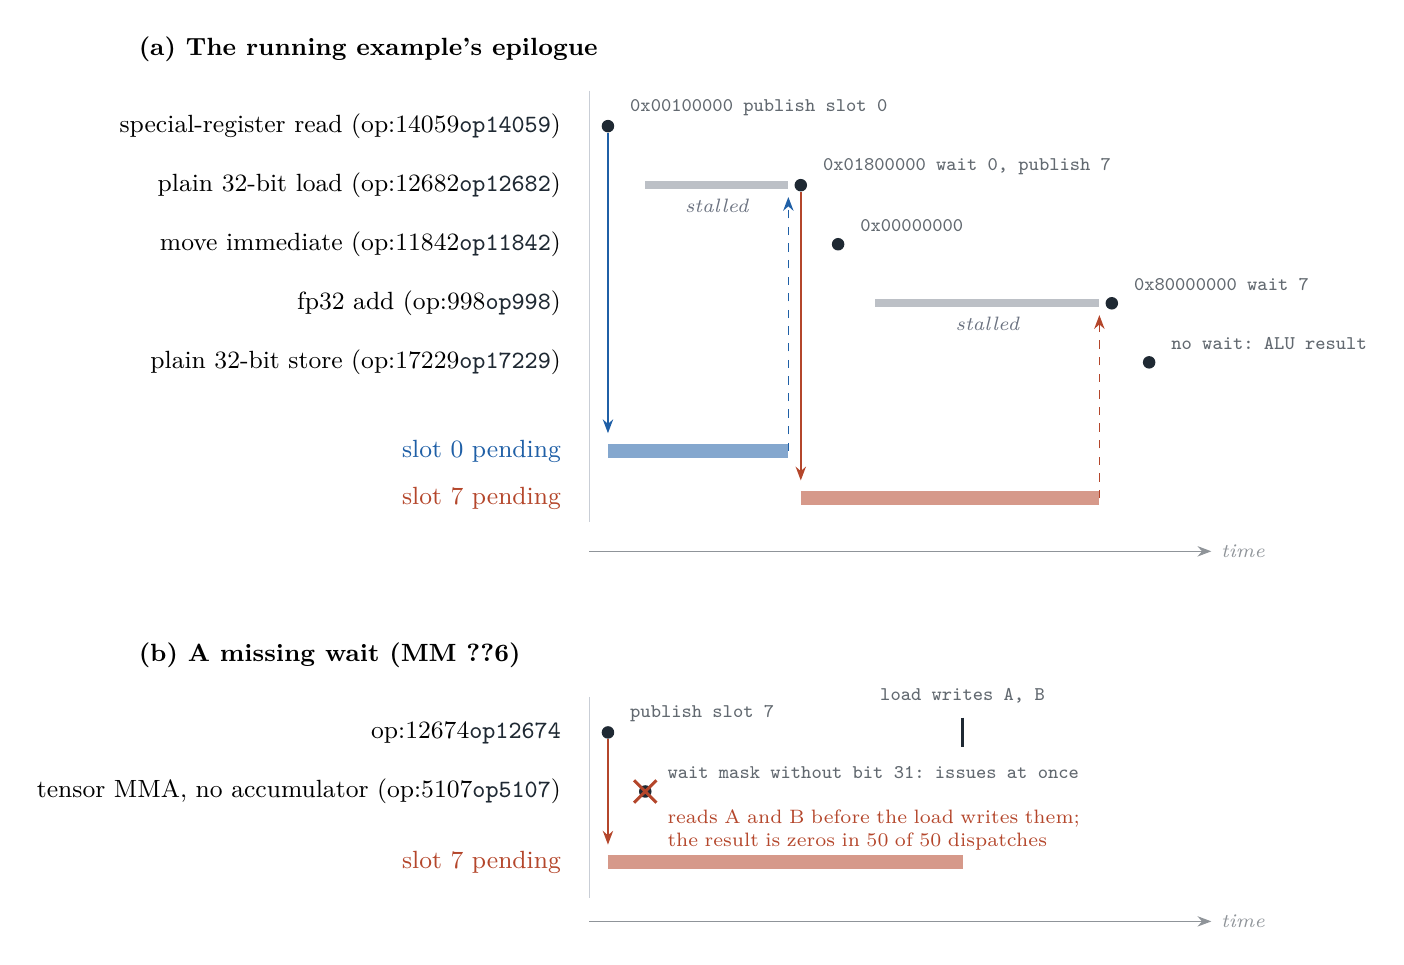
\begin{tikzpicture}[x=7.9mm, y=-7.5mm, font=\small,
    issue/.style={circle, fill=ink, inner sep=1.6pt},
    stall/.style={line width=3pt, color=apple!45},
    pend/.style={line width=5pt, color=#1!55},
    ins/.style={anchor=east, align=right, font=\small},
    ctl/.style={anchor=west, font=\scriptsize\ttfamily, text=ink!70}]
  \node[anchor=west, font=\small\bfseries] at (-7.4,-1.3) {(a) The running example's epilogue};
  % instruction rows
  \foreach \y/\n/\o in {0/special-register read/14059, 1/plain 32-bit load/12682,
      2/move immediate/11842, 3/fp32 add/998, 4/plain 32-bit store/17229}
    \node[ins] at (-0.3,\y) {\n\ (\opn{\o})};
  \draw[rule] (0,-0.6) -- (0,6.7);
  % slot lanes
  \node[ins, text=ours] at (-0.3,5.5) {slot 0 pending};
  \node[ins, text=native] at (-0.3,6.3) {slot 7 pending};
  \draw[pend=ours] (0.3,5.5) -- (3.2,5.5);
  \draw[pend=native] (3.4,6.3) -- (8.2,6.3);
  % issue points and stalls
  \node[issue] (i0) at (0.3,0) {};
  \draw[stall] (0.9,1) -- (3.2,1);  \node[issue] (i1) at (3.4,1) {};
  \node[issue] (i2) at (4.0,2) {};
  \draw[stall] (4.6,3) -- (8.2,3);  \node[issue] (i3) at (8.4,3) {};
  \node[issue] (i4) at (9.0,4) {};
  % publish and wait arrows
  \draw[->, ours, line width=0.6pt] (i0) -- (0.3,5.2);
  \draw[->, ours, line width=0.6pt, dashed] (3.2,5.5) -- (3.2,1.2);
  \draw[->, native, line width=0.6pt] (i1) -- (3.4,6.0);
  \draw[->, native, line width=0.6pt, dashed] (8.2,6.3) -- (8.2,3.2);
  % control words
  \node[ctl] at (0.5,-0.32) {0x00100000 publish slot 0};
  \node[ctl] at (3.6,0.68) {0x01800000 wait 0, publish 7};
  \node[ctl] at (4.2,1.68) {0x00000000};
  \node[ctl] at (8.6,2.68) {0x80000000 wait 7};
  \node[ctl] at (9.2,3.68) {no wait: ALU result};
  \node[font=\scriptsize\itshape, text=apple] at (2.05,1.35) {stalled};
  \node[font=\scriptsize\itshape, text=apple] at (6.4,3.35) {stalled};
  \draw[->, ink!50] (0,7.2) -- (10,7.2) node[right, font=\scriptsize\itshape] {time};

  \begin{scope}[yshift=-77mm]
  \node[anchor=west, font=\small\bfseries] at (-7.4,-1.3) {(b) A missing wait (MM~\mm{6})};
  \node[ins] at (-0.3,0) {\op{12674}};
  \node[ins] at (-0.3,1) {tensor MMA, no accumulator (\opn{5107})};
  \node[ins, text=native] at (-0.3,2.2) {slot 7 pending};
  \draw[rule] (0,-0.6) -- (0,2.8);
  \draw[pend=native] (0.3,2.2) -- (6.0,2.2);
  \node[issue] (j0) at (0.3,0) {};
  \node[issue] (j1) at (0.9,1) {};
  \draw[->, native, line width=0.6pt] (j0) -- (0.3,1.9);
  \node[ctl] at (0.5,-0.32) {publish slot 7};
  \node[ctl] at (1.1,0.68) {wait mask without bit 31: issues at once};
  \node[font=\scriptsize, text=native, align=left, anchor=north west, text width=52mm] at (1.1,1.15)
    {reads A and B before the load writes them; the result is zeros in 50 of 50 dispatches};
  \node[draw=native, cross out, line width=1.1pt, minimum size=7pt, inner sep=0pt] at (0.9,1) {};
  \draw[ink, line width=0.8pt] (6.0,-0.25) -- (6.0,0.25);
  \node[ctl, anchor=south] at (6.0,-0.33) {load writes A, B};
  \draw[->, ink!50] (0,3.2) -- (10,3.2) node[right, font=\scriptsize\itshape] {time};
  \end{scope}
\end{tikzpicture}
\caption{Late values and their waits, as the control words specify them. A dot is an instruction's issue; grey is
an instruction held at issue by its wait mask; a coloured bar is a scoreboard slot that a producer has published and
whose value has not yet arrived. A dashed arrow is a slot's arrival releasing its waiter. The control words in (a) are read
from the running example's bytes (the low 32 bits of operand 1: bits 20–23 publish slot + 1, bits 24–31 are the
wait mask). Panel (b) is the measured missing-wait experiment. Positions on the time axis are schematic; only the
order is measured.}
\label{fig:scoreboard}
\end{figure}


The per-form carriers (general loads, the 128-bit vector load, tensor load, the tensor MMA's
scattered mask bits, the 12-byte ALU wait bits, \op{592}) are tabulated in \cref{sec:scoreboard-publish-wait}. One carrier
is not in that table: in 14-byte stores byte9{[}5{]} is slot 7 in this compiler's encoder (\code{agxforge/g17/cc.py}). For
\op{12674}, MM~\mm{6} called the whole field bits 20--27, which includes the load's own wait mask; the fill slot is
bits 20--23 alone. The general-load field is measured through executed consumers
(MM~\mm{25.115}, MM~\mm{25.121}; \code{tools/g17emu.py} \code{load\_hazards}), the staging-file slot only through the decoder (MM~\mm{25.120.1}).

A decoder census gives the rule behind these. For 126 forms across 6,594 Apple programs, every instance's wait bits equal
exactly the slots its source registers are still pending on (\code{isa/g17-wait-mask-census.json}, MM~\mm{25.96}). It covers
stores: the \op{17256} uses every bit 24--31 (13,140 instances in a 314-object census, each one-hot
value present), which refuted an earlier "three-bit store limit" that was an encoder-table artifact (MM~\mm{6}). Tensor stores
are a separate class: all 876 \op{17257} and 118 \op{17258} instances carry a zero wait
byte, and the same-simdgroup MMA-to-tensor-store path is exact with no wait (measured, MM~\mm{6}).

The 8-byte \op{17229} also carries wait bits (15 corpus instances match their pending
slots, \code{isa/g17-wait-mask-census.json}; Apple's \code{tex2d-read} carries 0x1000010 on one, MM~\mm{25.146}). The "no wait bit" note
in \code{agxforge/g17/cc.py} describes this compiler's encoder, which has no carrier for them (\cref{app:a}).

Whether a consumer needs a wait depends on its producer:

\begin{itemize}
\item \emph{Not needed:} ordinary ALU to ALU. 52 of 52 ordered adjacent pairs of ordinary ALU instructions read the previous
  result bit-exactly with no wait (MM~\mm{25.90}, MM~\mm{6}).
\item \emph{Needed:} loads, imageblock reads, vector-load lanes, the packed half2 load, atomic returns, texture fetches and staging
  writes, for every consumer kind. An indirect load whose index is a loaded value read index 0 on every
  lane (1 of 32 right) until its operand 1 also named slot 7 (32 of 32; MM~\mm{25.104}, MM~\mm{25.90}). Shuffles and
  broadcasts of a loaded value read it early (\cref{sec:cross-lane-operations-consumers}). \op{11190}, \op{9986},
  \op{14047} and \op{590} do not interlock on a load (MM~\mm{25.133}), and a store takes its value register at issue
  (MM~\mm{25.96}).
\item \emph{Open:} whether an ALU consumer of an MMA result is interlocked. One ALU consumer placed directly after an MMA carried
  no wait and still read the result; no measured pair had an MMA producer (MM~\mm{6}, MM~\mm{25.90}).
\end{itemize}

Special-register reads fall between these. \op{14059} publishes a slot and Apple's compiler always waits on it, but a
slot-0 read is readable at distance 0 with no wait, and the wait has no measurable cost (measured, MM~\mm{25.117},
MM~\mm{25.121}; probe and counts in \cref{sec:read-latency-whether}).

An unwaited consumer could read the late value, if it arrived in time, or the register's previous contents. To tell these apart the producer's destination was pre-set. With a poison in it, the
four non-interlocking unary forms returned op(poison) on every lane; with a fresh register they returned op(0); a
negative control, an add with its load-wait bit cleared, read the poison on 1,024 of 1,024 lanes, so the instrument can
see a race (measured, MM~\mm{25.133}). The unwaited consumer reads the previous contents. Most observed failures
therefore read 0, and detecting them takes a sentinel or poison value; a zero-filled buffer cannot show them.

An atomic return published on the wrong slot was first found in decoded bytes and then confirmed on hardware
(MM~\mm{25.115}, \code{docs/g17-first-dispatch-trials.md}). This compiler's residency probe counts arrivals with \op{10094} and reads the returned old value. At S = 256 simdgroups every arrival read 1 (a returned 0, plus
one) while the departure maximum was 256. Two explanations fit: simultaneous same-address atomics combine and each requester sees the pre-combine
value (first recorded, later withdrawn), or the consumer read the register before the return arrived. The decoded bytes favoured the second. Marking the atomic's result late
gave its consumer, \op{10279}, this compiler's load-use wait, mask 0b10000000, slot 7, because this
compiler's loads fill slot 7. But the atomic's operand 1 bits 20--23 were 1: it filled slot 0, copied from Apple's
witnesses, where Apple's first consumer waits on bit 24 (120 of 120 corpus instances). The consumer waited on a slot the
atomic never touched. At larger S arrivals had agreed with departures, which had been read as the wait working; in fact
the arrivals were staggered enough that each return landed before its consumer read it. The deciding run changed only the slot. Publishing the atomic on slot 7
(the two programs differ in four bytes) gave an arrival maximum of 256, equal to the departure maximum, 3 of 3, while the
slot-0 arm read 1. Combining would not depend on which slot the return is published on.

Below Metal, the per-lane form behaved the same way. A 12-byte \op{10090}
publishing on slot 0 (operand 1 0x80100000) updated all 64 cells correctly and returned 0 to every lane, and it still
returned 0 with 64 independent two-byte moves inserted before the consumer, so added distance does not help. Changing two atomic bytes to publish on slot 7 (operand 1
0x80800000) returned all 64 old values.

Past eight groups the slot sequence Apple's compiler assigns is scheduler-chosen (twelve loads got 8, 1, 2, 3, 4, 4, 4,
4, 7, 7, 6, 5 in decoded values), so an emitter should use an explicit rule, such as K-step k in slot k mod 8; this
compiler's K = 256 lowerings use slot k mod 7, exact in 3 of 3 cases (MM~\mm{6}, \code{tools/tensorops-model/scoreboard-store-census.json}).
Reusing a slot after its named consumer has waited is safe (measured); reuse before that consumer is unmeasured and
forbidden (MM~\mm{0.14}, MM~\mm{6}). Loads and atomic returns work on slot 7 (measured), but a special-register read
publishing on slot 7 stored nothing, waited or not (measured, MM~\mm{25.121}; \cref{sec:read-latency-whether}).

The glossary's "the return fills scoreboard slot 7" for the uniform-address atomic and \op{11765} describes this
compiler's emission. Apple's corpus fills slots 0 and 1, and every first consumer waits on exactly that slot (25 of 25
for the uniform atomic, MM~\mm{25.115}).

Release acts per lane (\cref{ch:register-file}). A store naming one register as
both value and index, with the index slot releasing it, stores 0 (measured, MM~\mm{25.117}), and an instruction no lane
executes releases nothing (MM~\mm{25.95}).

\section{Barriers and fences}\label{sec:barriers-fences}

\op{447} is one six-byte instruction with scheduling class 3, MayStore, NotDuplicable and side effects.
Only operand 1, the scope immediate, changes with the Metal barrier (\cref{tab:barrier-scopes}; Apple's compiler emits,
\code{isa/g17-barrier-scopes.txt}).

\begin{longtable}{@{}lll@{}}
\caption{Encodings of the Metal threadgroup barriers.}\label{tab:barrier-scopes}\\
\toprule
Metal barrier & Bytes & Scope \\
\midrule
\endfirsthead
\tablecontinued{3}
\toprule
Metal barrier & Bytes & Scope \\
\midrule
\endhead
\code{threadgroup\_barrier(mem\_none)} & \code{075100060000} & 20 \\
\code{threadgroup\_barrier(mem\_device)} & \code{0f6900060000} & 154 \\
\code{threadgroup\_barrier(mem\_threadgroup)} & \code{275100060000} & 276 \\
\code{threadgroup\_barrier(mem\_texture)} & \code{876700060000} & 1144 \\
\code{threadgroup\_barrier(mem\_threadgroup\_imageblock)} & \code{475100060000} & 532 \\
\bottomrule
\end{longtable}

\code{mem\_threadgroup | mem\_device} emits two barriers, one per flag; \code{simdgroup\_barrier} emits nothing
(Apple's compiler emits, \code{isa/g17-atomic-semantics.json} barriers). Scopes 16, 528 and 1138 substituted for 276 each
carried a threadgroup-memory round trip (measured, the threadgroup-barrier notes in \code{tools/g17emu.py}).

Between simdgroups a threadgroup barrier is mandatory (measured, MM~\mm{14}, MM~\mm{17} rule 7). With no barrier, and with
\code{air.simdgroup.barrier} alone (which emits no instruction), a cross-simdgroup hand-off was wrong in 12 of 12 trials and
the consumer read the buffer's pre-write state. Every threadgroup-barrier variant
(execution-only, threadgroup memory, device memory, both) was correct in 12 of 12. A threadgroup store, barrier and load
also exchanged values below Metal, between the two simdgroups of a 64-thread group and in a half-full 32-thread second
group (measured, \code{docs/g17-first-dispatch-trials.md}).

For device memory between simdgroups, MM~\mm{14} observed that the execution-only barrier (scope 20) sufficed, and says so as "an observation about this chip, not a guarantee". The
emulator's race check (MM~\mm{25.197}) orders threadgroup memory across every threadgroup barrier but device memory only across scope 154,
and no measurement requires that restriction. Scope 276 (or any threadgroup barrier scope) is safe for threadgroup
memory between simdgroups, and scope 154 for device memory between simdgroups of one threadgroup. Scope 20 is not
established as safe for memory, and no threadgroup barrier orders anything across threadgroups (\cref{sec:ordering-across-lanes}).

A last-threadgroup pattern compared a threadgroup barrier with a device fence on hardware (MM~\mm{25.140.5}). Every threadgroup
writes a marker, crosses a barrier, and counts itself with \op{10094} on its rank-0
written buffer; the last threadgroup to arrive sums all markers. With the barrier at scope 154 the count was a perfect
permutation, yet the last threadgroup read stale markers: it summed 1,560 of 2,080 at 64 threadgroups and 123,408 of
131,328 at 512. Apple's compiler, given
\code{atomic\_thread\_fence(mem\_device, seq\_cst, thread\_scope\_device)}, emits \op{14156}, operands (0, 186), six
bytes \code{0f2b00060000}, no registers, and places one after the stores and one again inside the last threadgroup's region;
the loads stay ordinary. With those two fences both sums were exact. This compiler emits the same bytes (checked with
Apple's decoder). A fused attention merge built on the pattern was bit-exact at q0 = 0, 5, 128 and 271 over five
rounds each, with NaN-poisoned rows (costs in \cref{ch:performance}).

The imageblock barrier is the threadgroup barrier at scope 532 (\cref{sec:imageblock-per-core-tile}). The emulator admits it only for one simdgroup in
lockstep; more than one simdgroup was never witnessed (MM~\mm{25.145.2}). A barrier inside an exec-mask region is not modelled
there either (\code{tools/g17emu.py}).

Encoder-level barriers come from a static read of the AGX user driver (decoder, MM~\mm{25.141.20}); their costs are measured
in \cref{ch:performance}. A serial compute encoder emits a barrier token after every dispatch. A concurrent encoder emits
one only where \code{memoryBarrierWithScope:} asks; in a serial encoder that call only posts a notification. For a chain
where every dispatch depends on the last, both emit the same tokens. The token is one 32-bit command word, 0x60000160, OR
0x1000 when a pending flag is set; with its boolean arguments it ORs 0x400 or appends 0x60000502, both of unknown
function. The GPU drains at the token.

Hazard tracking never enters the per-dispatch path, since tracked and untracked buffers encode identically inside an
encoder. Consecutive compute encoders in one command buffer are merged, with an unconditional barrier after a concurrent
one. Tracked buffers with one serial encoder per token ran 0.2--0.3~ms per token faster than untracked buffers ordered by
an \code{MTLSharedEvent} between command buffers (\cref{sec:dispatch-encoder-command-buffer}), and untracked buffers
without ordering race (MM~\mm{0.15}).

Two dependent Submits on one queue below Metal, the second reading the first's output, computed exactly, also with a
program switch between them; and one Submit carrying two or three command records, each running a per-lane \code{+7}
read-modify-write on the same words, left 14 and 21 in every lane, so each record saw the previous record's result
(measured, \code{docs/g17-first-dispatch-trials.md}, "Dependent two-stage pure GPU pipeline" and "One to three dependent GPU
computations in one Submit").

\section{Atomics}\label{sec:atomics}

In the decoder (\code{isa/g17-atomic-family.toml}), 208 opcodes share the scheduling class of \op{10094} and flags
(classes 286 and 287 with flags 0x402002400 for device scope, class 329 with 0x402002800 for threadgroup scope) and one
operand skeleton, \code{[dest] imm imm [address] imm [index] imm imm imm [value] imm}, with parts present or absent. Five occur
in the corpus; 29 are reachable from one encoding of it by bit flips. The other 179 were never produced by single-bit
walks to saturation, 132,240 two-bit mutations, 1,365,504 three-bit mutations or 800,000 random encodings. Those
searches are bounded, so the 179 are not shown to be unreachable. Among the family's structural bits, byte4{[}0{]} returns old (to \op{10022}), byte4{[}1{]} selects a threadgroup GPR16 address over a device register pair (\op{11769}, no glossary entry),
byte5{[}2{]} selects an index register (\op{10090}), and byte6{[}2{]} leaves the family.

\begin{xltabular}{\linewidth}{@{}>{\hsize=1.18\hsize}Xl>{\hsize=0.85\hsize}XX@{}}
\caption{Atomic forms by address kind.}\label{tab:atomic-forms}\\
\toprule
Glossary name & Opcode & Address & Standing \\
\midrule
\endfirsthead
\tablecontinued{4}
\toprule
Glossary name & Opcode & Address & Standing \\
\midrule
\endhead
uniform-address atomic, returning old & \opn{10094} & device, uniform, byte offset in operand 6 & measured (below Metal, all operations below; MM~\mm{25.140.3}) \\
uniform-address compare-exchange, returning & \opn{10095} & device, uniform & measured (below Metal) \\
uniform-address no-return atomic, 32-bit & \opn{10022} & device, uniform & Apple's compiler emits \\
uniform-address no-return compare-exchange & \opn{10023} & device, uniform & Apple's compiler emits \\
per-lane-address atomic, returning & \opn{10090} & device, base + index register & measured (below Metal) \\
per-lane-address compare-exchange, returning & \opn{10091} & device, base + index register & measured (below Metal) \\
per-lane-address no-return atomic & \opn{10019} & device, per lane & Apple's compiler emits \\
64-bit no-return atomic, max/min & \opn{9996} & device & Apple's compiler emits \\
threadgroup atomic, returning old & \opn{11765} & threadgroup & measured (MM~\mm{25.115}) \\
threadgroup atomic, no return & \opn{11701} & threadgroup & measured (glossary) \\
\bottomrule
\end{xltabular}

Below, "the uniform atomic" means \op{10094} and "the per-lane atomic"
\op{10090}. "Uniform-address" refers only to the address. The uniform atomic
executes once per active lane, so 32 lanes add 32 and receive 32 distinct old values (measured, MM~\mm{25.140.3}). Its operand 6 is the address's byte offset: values 4, 8 and 16
moved the cell by 1, 2 and 4 words. Earlier claims called operand 6 a source lifetime ("16 writes nothing");
the probe had watched the wrong word (MM~\mm{25.140.3}).

The operation is a four-bit field, named by the decoder's operation operand. The decoder prints operand 2 as
0x40200 + code, so each executed operation's operand is 262656 + code. For the uniform atomic the four bits
are byte4{[}5{]}, byte5{[}3{]}, byte6{[}3{]} and byte7{[}7{]}; \cref{tab:atomic-operation-codes} reproduces all ten encodings Apple's compiler emits for
\code{atomic\_fetch\_\{add,sub,and,or,min,max\}} (both signednesses), \code{atomic\_exchange} and \code{atomic\_fetch\_xor} (decoder plus
Apple's compiler, \code{isa/g17-atomic-family.toml}) and gives the uniform atomic's shortest length for each code.

\begin{xltabular}{\linewidth}{@{}l>{\hsize=1.47\hsize}X>{\hsize=0.74\hsize}X>{\hsize=0.79\hsize}X@{}}
\caption{Atomic operation codes.}\label{tab:atomic-operation-codes}\\
\toprule
Code (operand) & Operation & Shortest length, uniform form & Executed below Metal, uniform form \\
\midrule
\endfirsthead
\tablecontinued{4}
\toprule
Code (operand) & Operation & Shortest length, uniform form & Executed below Metal, uniform form \\
\midrule
\endhead
0 (262656) & add & 10 & yes, returns consumed \\
1 (262657) & sub & 12 & yes \\
2 (262658) & exchange & 12 & yes \\
3 (262659) & compare-exchange: selects \op{10095} & 10 & yes \\
4 (262660) & unsigned min & 12 & yes \\
5 (262661) & signed min & 10 & yes \\
6 (262662) & unsigned max & 12 & yes \\
7 (262663) & signed max & 10 & yes \\
8 (262664) & and & 10 & yes \\
9 (262665) & or & 10 & yes \\
10 (262666) & xor & 12 & yes \\
12 (262668) & fp32 add, emitted by no tested Metal builtin & 10 & yes \\
\bottomrule
\end{xltabular}

Codes 11, 13, 14 and 15 do not decode. The same operand values name the per-lane operations, but the bits carrying them differ
by form and length: in the 12-byte per-lane atomic the fourth bit is byte11{[}4{]}, and a decoder sweep of that form maps the
assembler's three-bit operation with byte11{[}4{]} set and clear onto these codes (\code{docs/g17-first-dispatch-trials.md},
"Per-lane AND old-value return"). An authored "OR" with byte11{[}4{]} set executed exchange, updating every cell to the new
value; clearing that one bit gave operand 262665 and OR (measured). The "eight unassigned raw operation
codes" of \code{isa/g17-atomic-semantics.json} were read off one witness's field placement and are retracted
(\code{isa/g17-atomic-family.toml}; \cref{app:a}).

Each case below ran below Metal, in relaxed order within one dispatch, in two fresh processes with output guards
(\code{docs/g17-first-dispatch-trials.md}; \code{isa/g17-atomic-family.toml}).

\begin{itemize}
\item 64 lanes adding to one cell left exactly the sum (5 to 69 with +1; 5 to 2085 with lane i adding i + 1), and
  every lane received a distinct old value; with lane-varying addends the returned values form a unique chain through all
  64 lanes. Two simdgroups' elected lanes on one uniform atomic received non-overlapping intervals (5--36 and 37--68).
\item Integer operations matched their Metal definitions, including 32-bit modular sub (5 - 32 - 32 = 4294967237), signed against unsigned
  extrema on 0xFFFFFFFF and 0x80000000, and exchange.
\item Compare-exchange takes the register tuple (desired, expected), established from the compiler's witness; matched and
  failed compares both returned the old value.
\item The fp32 add (code 12), uniform and per-lane, returned 1.0f and 2.0f for 1.0f + 1.0f + 1.0f, leaving 3.0f; 64
  per-lane updates of 1.0f from 1.0f reached 65.0f and returned 1.0f through 64.0f once each. Each update rounds to
  nearest even: half-ULP ties left an even mantissa unchanged and moved an odd one up once (0x3F800001 to 0x3F800002) and
  no further. Subnormal inputs, operands and results flush to zero. A quiet NaN seed 0x7FC12345 was returned raw to its
  first caller and then stored as canonical 0x7FC00000; $-0$ plus $+0$ returned $-0$ and stored $+0$; infinities were preserved.
\end{itemize}

Atomics have been run only on the rank-0 buffer, through Metal and below it; this compiler refuses an
atomic whose identity base and binding rank disagree (\code{agxforge/g17/cc.py}; MM~\mm{25.140.3}). Threadgroup atomics need a
threadgroup region, which only an ordinary threadgroup load or store provisions (\cref{sec:threadgroup-memory}).

Atomic return values are late; the fill slot is operand 1 bits 20--23 minus 1, and slot choice is in \cref{sec:scoreboard}. The 10-byte uniform atomic also releases its value: operand 9 is the value's lifetime and only 16 is
representable, so a second atomic sharing a constant read 0 (A{[}0{]} = 0 against 24; measured by this compiler's fuzzer,
MM~\mm{25.144.6}, \code{agxforge/g17/cc.py}); a value read again must be copied first.

Validation with the return value consumed:

\begin{itemize}
\item The uniform atomic was validated below Metal for all eleven of its operations in \cref{tab:atomic-operation-codes} (every code except 3), each under two-group
  contention with the returned old value consumed; \op{10095} at match and
  mismatch. Through Metal it was validated for add, in the residency probe (MM~\mm{25.115})
  and the compiler's wave-broadcast program (\code{agxforge/g17/cc.py}).
\item The per-lane atomic ran below Metal update-only for add, and, or, sub, xor, signed and unsigned min and max, exchange and
  fp32 add; returns through slot 7 for add (also contended, both fixed and lane-varying addends), and, or, sub, xor and
  fp32 add (also contended, half-ULP and NaN cases). Compiler-generated 12-byte programs for add, and, or, sub and xor
  passed with a direct indexed-store consumer, plus an ordinary add consumer for add and xor.
\item \Op{10091} passed with a hand-authored slot-7 return (one matching and 63 failing compares), then with
  compiler-generated programs at index placements R0, R1, R5, R7 and R12 (ten Submits); other placements are decode-checked
  predictions, and placement 13 is refused.
\item \Op{11765} was dispatched through Metal with its return consumed; its \op{11667} consumer had read both returns with an empty wait mask until fixed, where Apple waits 10 of 10 (MM~\mm{25.115}).
\item Not validated are per-lane min and max returns, unsigned long-form returns, other consumer shapes (refused by this
  compiler), 64-bit atomics (\op{9996}, compiled only), and any atomic on a buffer other
  than rank 0.
\end{itemize}

An atomic does not order other memory (\cref{sec:barriers-fences}); ordering ordinary stores through an atomic needs
\op{14156}. The emulator does not
track atomics in its race check and does not model acquire or release through atomics or the fence, so it refuses any
program that synchronizes threadgroups through an atomic counter (MM~\mm{25.197}).

\section{Ordering by scope}\label{sec:ordering-across-lanes}

\subsection*{Lanes of one simdgroup}

\begin{itemize}
\item Program order holds on one scoreboard: a store followed by a load in one simdgroup needs no fence, as two separately
  generated bodies joined at a shared buffer showed, including a cross-lane stress where each lane read another lane's
  write (measured, MM~\mm{13}). Late values still need the consumer's wait.
\item Same-address stores with \op{17229}: the lowest active lane wins, by lane and not by value (all
  lanes: lane 0; lanes 0--15 under an exec region: lane 0; odd lanes: lane 1; reversed values: lane 0; five runs each;
  measured, MM~\mm{25.145.4}, \code{isa/g17-execution-storewinner-results.json}).
\item Registers never cross a simdgroup: a cross-simdgroup \code{simd\_shuffle} returns the caller's own value, 256 of 256
  (measured, MM~\mm{14}).
\end{itemize}

\subsection*{Simdgroups of one threadgroup}

A threadgroup barrier is the only mechanism at this scope (\cref{sec:barriers-fences}); same-value writes by
several simdgroups are harmless by construction (no schedule changes the bytes), and shipped code relies on that: the fused attention appends a
new K/V row from every simdgroup of every threadgroup and each reads its own copy back (modelling rule, MM~\mm{25.197}).

\subsection*{Threadgroups of one dispatch}

MM~\mm{0.14}'s map says "cross-threadgroup handoff requires a
dispatch boundary". It was written about tensor fragment hand-offs before any in-dispatch mechanism had been measured.
MM~\mm{25.140.5} and MM~\mm{25.141.1} have since measured two, so the dispatch boundary is the safe default, and fenced
atomic patterns also work within one dispatch.

Device stores from one threadgroup are visible to another in the same dispatch after \op{14156} on the writer side and
again on the reader side (measured for the last-threadgroup pattern, MM~\mm{25.140.5}); a threadgroup barrier at any
scope does not make them visible. An atomic count decides which threadgroup is last (atomicity is measured in
\cref{sec:atomics}).

The last-threadgroup pattern needs no forward progress, because no threadgroup waits; whoever counts last does the
follow-on work. Any pattern that waits needs the producer resident. In the forward-progress probe the first resident
wave spun to its cap before the producer, dispatched last, ran at all (measured, MM~\mm{25.141.1}; the grid sizes and
counts are in \cref{sec:forward-progress-in-order}). A grid barrier among resident
threadgroups, fenced and capped, kept totals exact in every run and never reached its cap (measured, MM~\mm{25.141.1}).
MM~\mm{17} rule 40 allows a wait on another threadgroup only when every participant fits in measured resident capacity
at the kernel's own register and threadgroup-memory use, with capped spins and work pulled from an atomic queue. The barrier took
133.1~µs per 32~MB phase against 120.8~µs with dispatch boundaries (\cref{sec:dispatch-encoder-command-buffer}).

The residency of 1,024-thread threadgroups is unresolved. The forward-progress probe implies at least
10 co-resident per core, while the driver formula gives 3 (MM~\mm{25.141.1}, MM~\mm{25.141.20}); no residency count may be assumed, and
a spin-waiting grid of them must not be sized from either number (\cref{sec:residency-occupancy-rules}, rule 5).

\subsection*{Dispatches}

In the tested configurations threadgroups were dispatched in order and no spinning threadgroup gave way to a producer
dispatched after it (MM~\mm{25.141.1}; \cref{sec:forward-progress-in-order}). No guarantee of that behaviour has been
established, so a program cannot depend on preemption. A serial encoder places
a barrier token after every dispatch; a concurrent encoder lets a dependent kernel start early, but its threadgroups queue
behind all of the producer's, so only the producer's last-wave tail overlaps (measured, MM~\mm{25.141.1}; costs \cref{ch:performance}).
A concurrent encoder needs \code{memoryBarrierWithScope:} before every dispatch that reads
an earlier dispatch's output.

A line of a write-combined buffer that the GPU read recently stays stale in the GPU's L2 after the CPU updates it
(measured, MM~\mm{0.15}).

\textbf{Not known.} The cross-simdgroup winner of same-address stores; whether an execution-only barrier orders device
memory by design; threadgroup barriers in partial groups of other sizes and with inactive lanes accessing memory; why a
special-register read on slot 7 stores nothing; signaling NaNs and other NaN payloads in the fp32 atomic add; acquire and
release semantics in general (only the fence-count-fence pattern is measured); the function of the barrier-token
variants 0x400 and 0x60000502; the ordering of other command shapes below Metal, and whether command records can
overlap.

\textbf{Evidence.} MM~\mm{0.8}, MM~\mm{0.14}, MM~\mm{0.15}, MM~\mm{6}, MM~\mm{13}, MM~\mm{14}, MM~\mm{17} rules 4, 7, 35 and 40, MM~\mm{25.90}, MM~\mm{25.95}, MM~\mm{25.96},
MM~\mm{25.104}, MM~\mm{25.115}, MM~\mm{25.117}, MM~\mm{25.120.1}, MM~\mm{25.121}, MM~\mm{25.133}, MM~\mm{25.140.3}, MM~\mm{25.140.5}, MM~\mm{25.141.1}, MM~\mm{25.141.20},
MM~\mm{25.144.6}, MM~\mm{25.145.2}, MM~\mm{25.145.4}, MM~\mm{25.146}, MM~\mm{25.197}; \code{isa/g17-barrier-scopes.txt}, \code{isa/g17-atomic-family.toml},
\code{isa/g17-atomic-semantics.json}, \code{isa/g17-wait-mask-census.json}, \code{isa/g17-execution-storewinner-results.json},
\code{docs/g17-first-dispatch-trials.md}, \code{agxforge/g17/cc.py}, \code{tools/g17emu.py},
\code{tools/tensorops-model/scoreboard-store-census.json}.

\chapter{The tensor unit}\label{ch:tensor-unit}

The tensor unit (Apple's "neural accelerator") performs one 16 × 16 × 16 matrix multiply-accumulate
per instruction, \code{D = C + A.B} or \code{D = A.B}: 4,096 multiply-accumulates and 8,192 floating-point operations per issue,
with one logical tensor-issue slot per SIMD and four per core (measured, MM~\mm{0.1}, MM~\mm{8}). It is distinct from the older 8 × 8 simdgroup-matrix engine (\cref{sec:legacy-simdgroup-matrix-engine}) and from the Apple Neural
Engine, which this reference does not cover.

The instruction's operands are register tuples spread across the 32 lanes of one simdgroup. Each lane holds 8 of a
tile's 256 elements in fixed slots. Tensor loads are per-lane gathers at addresses computed by ordinary ALU code, and
that arithmetic produces the layout; nothing reshapes the tile on the way (\cref{sec:fragment-layouts,sec:tensor-memory-path}).

\leadhead{Notation.}

\begin{itemize}
\item \textbf{MMA}: one tensor multiply-accumulate instruction. "With-C" forms read an accumulator C; "no-C" (from-zero) forms
  do not.
\item \textbf{The 16-bit MMA}: \op{5106}, the form most measurements use; the other
  nine forms are named in full (\cref{sec:instruction-family}).
\item \textbf{Tile}: a 16 × 16 matrix. A is M × K (16 × 16), B is K × N, C and D are M × N. Larger GEMMs are grids of tiles.
\item \textbf{Fragment}: the part of one tile held by one lane. Every lane holds 8 logical elements of a tile, numbered by a
  \textbf{slot} \code{j} in 0..7; lane \code{l} is 0..31 (SR130, the lane index within the simdgroup, \cref{ch:special-registers}).
\item \textbf{Tuple}: the aligned group of consecutive registers holding a fragment (widths and legal bases in
  \cref{tab:fragment-registers}).
\item \textbf{Accumulator group}: an 8-register fp32 or int32 tuple (C and D).
\item \textbf{Modifier}: the immediate that follows every register operand in the decoded form, carrying the operand's
  lifetime bits (release and keep). The general rule is in \cref{ch:register-file}, the tensor-specific use in \cref{sec:modifiers-keep-flag}.
\item \textbf{Feed}: using one MMA's D as a later MMA's A, B or C without a store.
\item \textbf{Memory bridge}: storing D to row-major memory with a tensor store and reloading it with a tensor load.
\item \textbf{\enquote{pos} and \enquote{pos\_b} layouts}: the two (lane, slot) maps of \cref{sec:fragment-layouts}.
\item \textbf{Silent}: a violation produces wrong or zero results with no error from compiler, driver or API.
\end{itemize}

\code{rotl1(x)} and \code{rotr1(x)} rotate a four-bit row index left or right by one bit, and \code{RNE32(x)} rounds x
to fp32, nearest-even. Provenance tags follow \cref{sec:read-this-document}, with the decoder tag written
\emph{decoder only}.

\section{Access through Metal}\label{sec:it-reached}

Metal 4's TensorOps API reaches the unit through a bitcode library linked at native compile time (Apple's compiler
emits, MM~\mm{1}).

\begin{enumerate}
\def\labelenumi{\arabic{enumi}.}
\item \code{mpp::tensor\_ops::matmul2d<descriptor, execution\_simdgroups<N>>::run} is header code. It calls \code{extern "C"} symbols
  named \code{\_\_tensorops\_impl\_matmul2d\_op\_run\_<left>\_<right>\_<dest>[\_v2]}, declared in the \code{air.externally\_defined}
  section, so a TensorOps kernel's AIR holds only a call to one of these symbols.
\item The symbols resolve at native compile time from
  \code{MetalPerformancePrimitives.framework/Resources/libTensorOps.rtlib}, an ar archive of 1,970 air64\_v28 bitcode
  members, 1,475 of them \code{matmul2d\_op\_run\_*}.
\item Inside the library, \code{air.supports\_family(i32 1010)} (\code{MTLGPUFamilyApple10}: M5 and A19 Pro) selects
  \code{air.simdgroup\_matrix\_16x16x16\_multiply\_accumulate}; family 1009 selects the older
  \code{air.simdgroup\_matrix\_8x8\_multiply\_accumulate}.
\item The 16 × 16 × 16 intrinsic lowers to one native instruction, \op{5106}, or
  a sibling from \cref{sec:instruction-family}.
\end{enumerate}

The AIR intrinsic surface is
\code{16x16x16\_multiply\_accumulate.f.f.v8f32.\{v8f16|v8bf16|v8f32\}.\{v8f16|v8bf16|v8f32\}.v8f32} (nine A/B combinations, fp32
accumulator only) plus the integer widening form \code{.\{s|u\}.\{s|u\}.v8i32.v8i8.v8i8.v8i32}. A fragment is a per-lane
\code{<8 x T>} value (Apple's compiler emits, MM~\mm{1}). Hand-written AIR reaches the intrinsic directly, which is how the
saturating int8 form, fp8 and the scaled spelling were reached (\cref{sec:instruction-family,sec:quantized-formats}).

\code{relaxed\_precision} selects the mixed float forms. Without it, the mixed float intrinsics fall to the legacy
datapath with a different layout; with it they reach \op{5098}, \op{5100} and \op{5104}, and the no-C fp32-A form
\op{5101}. It is inert for forms already native (Apple's compiler emits, measured, MM~\mm{17} rule 29).

Apple's library body changes with the simdgroup count (Apple's compiler emits, MM~\mm{25.93}). At \code{execution\_simdgroups<1>} the slot-29
system-register vector is \code{[52]} and the body reads only SR130; at \code{<2>} and \code{<4>} it is \code{[52, 53]} and the body also
reads SR133 (the simdgroup index within the threadgroup). The N > 1 body is a per-simdgroup partition: no barrier, no
threadgroup memory, only the 16-bit MMA for the matrix work, plus offset arithmetic (\op{17016}, \op{426}, \op{10286} and \op{10285}). How many MMAs each simdgroup runs is a library tiling choice: for 32 × 32 × 64, \code{<2>} halves 32 to
16 and \code{<4>} stays at 16; for 64 × 64 × 64, \code{<2>} keeps 64 and \code{<4>} halves to 32.

The API imposes rules of its own that the hardware does not (measured unless marked):

\begin{itemize}
\item \code{execution\_simdgroups<N>} must equal the simdgroups launched. A narrower scope silently returns zero (MM~\mm{14},
  MM~\mm{17} rule 8).
\item \code{reduce\_rows} and \code{reduce\_columns} refuse to compile at \code{execution\_simdgroups<2>} or above; an input cooperative
  tensor must be single-simdgroup and cannot be transposed, although the hardware transposes a fed operand (Apple's
  compiler, MM~\mm{12}, MM~\mm{0.9}).
\item Apple's header \code{MPPTensorOpsMatMul2dImpl.h} (macOS 26.4 SDK, lines 3763–3765) asserts that M and N are multiples of
  8 and at least one is a multiple of 16. Per-lane capacity \code{M*N/32} is therefore always a multiple of 4 (4, 8, 12,
  16, 20, 24 \dots{}); \code{24x24} fails the assert (Apple's compiler, MM~\mm{12}).
\item The Metal 4.1 fp8 path is blocked at four points on this OS: the frontend needs \code{-std=metal4.1}, the loader refuses the
  4.1 language tag and the AIR 2.9 target, the OS \code{libTensorOps.rtlib} has no fp8 or scale symbols, and the OS tensor
  library lacks the builtins. Hand-written AIR still reaches fp8 (MM~\mm{11}).
\end{itemize}

\textbf{Evidence.} MM~\mm{1}, MM~\mm{12}, MM~\mm{14}, MM~\mm{17}, MM~\mm{19}, MM~\mm{25.93}.

\section{MMA instruction forms}\label{sec:instruction-family}

Every admitted tensor MMA is 10 bytes, scheduling class 172 for the 16-bit MMA, and writes an 8-register fp32 or int32
destination (decoder and measured, MM~\mm{0.3}, MM~\mm{2}). In every Apple-emitted with-C instance D and C are the same tuple
(481 of 481, MM~\mm{2}). No execution of an out-of-place form (D a different tuple from C) is recorded.

\widetable
\begin{xltabular}{\linewidth}{@{}l>{\hsize=0.69\hsize}X>{\hsize=0.69\hsize}Xl>{\hsize=1.20\hsize}X>{\hsize=1.26\hsize}X>{\hsize=1.18\hsize}X@{}}
\caption{The ten admitted tensor MMA forms, all ten executing on hardware (measured, MM~\mm{2}, MM~\mm{5}, MM~\mm{11}).}\label{tab:mma-forms}\\
\toprule
Form & A: type, tuple & B: type, tuple & D & With C & No C (from zero) & Arithmetic \\
\midrule
\endfirsthead
\tablecontinued{7}
\toprule
Form & A: type, tuple & B: type, tuple & D & With C & No C (from zero) & Arithmetic \\
\midrule
\endhead
16 × 16 & half or bfloat, 4 & half or bfloat, 4 & fp32, 8 & \op{5106} & \op{5107} & exact products, the tree of 
\cref{sec:arithmetic-semantics-supported} \\*
16 × fp32 & half or bfloat, 4 & fp32, 8 & fp32, 8 & \op{5104} & \op{5105} & fp32 operand truncated to 10 fraction bits \\*
fp32 × 16 & fp32, 8 & half or bfloat, 4 & fp32, 8 & \op{5100} & \op{5101} & fp32 operand truncated \\*
fp32 × fp32 & fp32, 8 & fp32, 8 & fp32, 8 & \op{5098} & \op{5099} & both operands truncated \\*
int8 & signed or unsigned int8, 2 & signed or unsigned int8, 2 & int32, 8 & \op{10384} & \op{10385} & exact products, mod $2^{32}$ by default; saturating variant below \\*
\bottomrule
\end{xltabular}

Decoded, the 16-bit MMA's operands are (decoder only, MM~\mm{2})
\code{D:GPR32tup8, imm, imm, A:GPR32tup4, imm, imm, B:GPR32tup4, imm, imm, C:GPR32tup8, imm, imm}; its no-C sibling drops the
C triple; the running example's first MMA (\cref{sec:one-program-ir}) is this no-C form decoded and annotated. Operands are
numbered from 0 (D). Each register is followed by two immediates: the first is its modifier
(\cref{sec:modifiers-keep-flag}; operands 1, 4, 7 and 10), and the second after A and after B carries that operand's type code
(operands 5 and 8); the second after D (operand 2) carries the saturation flag on the int8 form. Register fields are encoded in units of the tuple width, so a tuple must be
aligned. An encoder must refuse an unaligned base and must decode its output back to the same opcode, length and
operands; \code{mmaenc} once rounded an odd index silently (MM~\mm{0.4}, MM~\mm{2};
\cref{sec:admission-decodes-executes}).

\begin{xltabular}{\linewidth}{@{}llX@{}}
\caption{Operand type codes of the tensor MMA. The first row gives the field's position for A and for B.}\label{tab:mma-type-codes}\\
\toprule
Type & Code & Where \\
\midrule
\endfirsthead
\tablecontinued{3}
\toprule
Type & Code & Where \\
\midrule
\endhead
float (fp32) & 1 & A at byte6{[}2{]}, B at byte7{[}6{]} \\*
half & 2 &  \\*
bfloat & 3 &  \\*
unsigned int8 & 11 &  \\*
signed int8 & 75 &  \\*
\bottomrule
\end{xltabular}

A and B each carry a type code (\cref{tab:mma-type-codes}; decoder and measured, MM~\mm{0.3}, MM~\mm{2}), and a
transpose flag adds 32 to it (byte8{[}2{]} for A, byte8{[}3{]} for B). The signedness of
an int8 operand is selected independently for A and B. A transpose changes only how a fragment is read:
all four flag combinations compute exactly \code{D = C + A.B}, a transposed operand's loads keep the same index register
and displacements, and transposition has no measured issue cost (measured, MM~\mm{3}, MM~\mm{8}).

In the 10-byte MMA (decoder and measured, MM~\mm{0.4}, MM~\mm{2}), byte8{[}1{]} selects the no-C
sibling; byte5{[}7{]} makes B fp32; byte8{[}4{]} makes A fp32 on the float forms; byte6{[}0{]} selects the int8 family; byte0{[}7{]}
is bit 0 of the destination tuple index (40 of 40 instructions in six objects match \code{byte0[7] == N \& 1}), not a flag;
flags bits 24–31 are the scoreboard wait mask (\cref{sec:ordering-enable}; carriers in \cref{sec:scoreboard-publish-wait}). Bytes should be
built from the repository's JSON field map, which classifies all 80 bits of the 16-bit MMA (39 in mapped fields, 25
structural, 16 inert); \code{mmaenc.py}, which uses it, round-trips 800 of 800 compiler-emitted MMAs byte for byte
(MM~\mm{2}, MM~\mm{6}).

A single-bit census (measured, MM~\mm{2}) dispatched all 80 one-bit variants of the 16-bit MMA: none was
refused by the driver or faulted, every decoder-inert bit was hardware-inert, and every flags-word bit was inert on a
single MMA except byte0{[}3{]} (the slot-7 wait bit). Of the decoder-refused one-bit variants, six left the accumulator
unchanged (D == C) and eight changed the result, so decoder refusal does not predict what the hardware executes. No encoding property
separates the eight from the six (decoder only, MM~\mm{25.36}). Authored forms Apple's compiler never emits (swapped A/B
tuples, both transposes, A reinterpreted as bfloat) execute as layout and arithmetic predict (measured, MM~\mm{2}, MM~\mm{15}).

On the int8 MMA, \op{10384}, and its no-C form, \op{10385}, byte8 carries
three independent bits: bit 2 transposes A, bit 3 transposes B, bit 4 saturates (measured, MM~\mm{11},
MM~\mm{25.42}). Apple's compiler bytes are 0x40 untransposed and 0x44 with A transposed; with saturation 0x50 and 0x54. In
the decode, transposing A moves operand 5 only, transposing B moves operand 8 only, and saturation moves operand 2
(immediate 9 to 41) identically under all four transpose combinations; both int8 forms accept the bit (decoder only,
MM~\mm{25.11}).

Hand-written AIR reaches the saturating form through \code{widening\_multiply\_accumulate\_saturate}, which lowers
to the int8 MMA with the bit set. \code{libTensorOps.rtlib} contains no string containing \code{saturate}, so Apple's
library never emits it (Apple's compiler, MM~\mm{11}). The public matrix interfaces declare no saturating operation
either: the MPP headers of the macOS 27.0 SDK (where \code{matmul2d\_descriptor::mode} is \code{multiply} or
\code{multiply\_accumulate}) and the \code{metal\_simdgroup\_matrix}, \code{metal\_tensor} and
\code{metal\_cooperative\_tensor} headers of the Metal 32023 toolchain contain no string \code{saturat} (header search,
2026-10-04).

The signedness of the int8 intrinsic is spelled in its AIR suffix. In the four-letter suffix A's signedness is letter
2 and B's letter 3, and the parser ignores the outer letters; in the two-letter form A is always signed, so unsigned A
cannot be spelled (MM~\mm{11}, MM~\mm{20}).

The saturating form issues at the wrapping form's rate to three places and uses the same register classes
(measured, MM~\mm{11}). \code{mmaenc} emits it with C (\code{mmaenc.mma(saturate=True)}, byte-exact
against Apple's \code{\_saturate} spelling) and refuses the no-C saturating form, whose bytes 6 and 7 differ. In a
coverage count over 152 kernels the encoder reproduces 405 of 413 MMAs, and the 8 it misses are the no-C saturating
ones (this compiler, MM~\mm{15}, MM~\mm{25.11}). Its saturating chains ran on hardware (MM~\mm{25.89}); how a chain
clips is in \cref{sec:arithmetic-semantics-supported}.

Apple's tables declare 132 matrix forms by scheduling class and 535 by opcode range (the two counts measure
different things; \cref{app:a}), but only the ten above are decoder-admitted, all of them 32-bit-accumulator forms
(decoder only, MM~\mm{2}, MM~\mm{0.3}, MM~\mm{25.6}).

\begin{itemize}
\item Admission is gated on the CPU name passed to the decoder: g17s, g17g and g18 admit the same ten; g17, g16, g16s,
  g16g, g15 and g15s decode the same bytes as unrelated instructions (exhaustive three-flip sweep). The other declared
  forms are a bounded negative: none was reached within three flips of the ten seeds, nor from 1.1 million flip
  candidates plus a five-deep search (decoder only, MM~\mm{2}, MM~\mm{25.4/F4}).
\item Exactly three operand classes are exclusive to the accelerator across all declared accelerator opcodes: class 335 (the
  8-word tuple, D of every 32-bit-accumulator form, 18 of 18), class 159 (the 4-word tuple, D of every
  16-bit-accumulator form, 36 of 36) and class 41 (the 2-word tuple) (decoder only, MM~\mm{25.6}).
\item The 36 narrow-accumulator rows, \op{5108} through \op{5143}, use the same operand classes and counts as forms that decode,
  yet none was admitted from 1.1 million mutations plus a five-deep frontier, under any CPU name, and no witness emits
  one. Do not select or synthesize them (bounded negative, MM~\mm{25.13}).
\item The 475 \code{\_shifted} declarations use none of the three accelerator classes; they are a structurally different family
  that shares scheduling classes 174 and 175 (decoder only, MM~\mm{25.6}).
\item No admitted form accumulates in 16 bits. Hand-written AIR with a half accumulator lowers to the 16-bit MMA with
  eight \op{1004} before and eight \op{1016} after (the code section grows
  from 42 to 52 instructions); a bfloat accumulator uses the 16-bit MMA with bit operations and eight \op{1048} (62 instructions) (Apple's compiler emits, MM~\mm{25.13}).
\item No declared MMA form has a scale operand in Apple's tables (decoder only, MM~\mm{11}).
\end{itemize}

\textbf{Not known.} A structural bit-71 variant of the int8 widening MMA that Apple's decoder \code{agx3dis} does not
admit runs bit-exact in all three kernels that carry it; its 10-byte boundary is settled, its field meaning and decoder
identity are open (MM~\mm{20}, T11).

\textbf{Evidence.} MM~\mm{0.3}, MM~\mm{0.4}, MM~\mm{2}, MM~\mm{11}, MM~\mm{15}, MM~\mm{25.4/F4}, MM~\mm{25.6}, MM~\mm{25.11}, MM~\mm{25.13}, MM~\mm{25.36},
MM~\mm{25.42}.

\section{MMA operand modifiers}\label{sec:modifiers-keep-flag}

The modifier enum \{0, 16, 32, 48\} (weight 16 \textbf{release}, weight 32 \textbf{keep}; decoder only, MM~\mm{6}) and the destructive
release semantics are defined in \cref{sec:release-does}.

The modifier after A or B is 16 exactly when that tuple is not read again (Apple's compiler
emits, MM~\mm{6}). The running example (\cref{sec:one-program-ir}) shows the pattern: each fragment is read by two MMAs,
the first keeps it (0) and the second releases it (16). Because the release is destructive, a release set while any
later consumer remains loses the fragment. A later reader may assume neither zero nor the old value (\cref{sec:release-does}). The release acts per lane, and
nothing reclaimed a released register within the measured bound (MM~\mm{25.95}).

Whether a release point is safe depends on where the fragment came from, and this compiler's lowering once placed it
wrongly (this compiler, measured, MM~\mm{25.89}). With three accumulators free, \code{tlower} ran a 2 × 2 stage as two accumulator groups and released A
at its last read within each group. That is correct for an A loaded from memory, which each group reloads, and wrong
for a register-fed A, which has no memory copy: the second group read released registers and its tile came back all
zero. The fix releases a register-fed A at the last group that reads the row. \code{agxforge/g17/tensorlife.py}
(\code{released\_reads}) decodes every emitted body and refuses any MMA read of a released, unrewritten register; it fires on
the faulty program at exactly the two faulty issues and passes all 720 Apple corpus programs that contain MMAs.

The destination keep flag (\code{0x20}, \code{mmaenc} keyword \code{more}) is the keep bit of operand 1, the modifier after
D: byte4 bit 3, instruction bit 35 (\code{auth.carriers(5106, 1)[5] = [(4, 3, 0)]}) (decoder only, MM~\mm{6}, MM~\mm{25.22}). The
destination modifier carries keep and never release (\code{carriers(5106, 1)} has no bit-4 entry).

Apple's compiler sets it exactly when the next MMA writes the same destination tuple: in a run of n MMAs accumulating
into one tuple, the first n-1 carry it and the last does not (Apple's compiler emits, MM~\mm{25.22}). Flipping it had
no effect on a single MMA or on a two-step chain (measured, MM~\mm{2}); of keep and release it is the conservative
bit, since it only asserts reuse (MM~\mm{6}). An emitter should copy Apple's rule. Clearing the bit where Apple sets it
had no measured cost, and setting it where the next MMA does not reuse the tuple was never tested.

Over 2,192 MMAs in 140 programs
(1,093 carry the flag), "the next MMA reuses the tuple" has precision 100 percent (1,093 of 1,093) and recall 99.7
percent (1,093 of 1,096), while "some later MMA reuses it" has recall only 69.0 percent (MM~\mm{25.22}). A larger census
has zero counterexamples among 540,396 flag-set instances and 155,963 counterexamples to the converse (MM~\mm{6}). The three
misses in the 2,192-MMA census are one pattern: kernel \code{conv-c64k1}, destination D=3382, with the same 16 intervening
\op{595} instructions (MM~\mm{25.22}).

The accumulator's own modifier is operand 10 (the accumulator itself is operand 9). No field maps to it: the field
map's single-bit census classifies all 80 bits of the 16-bit MMA and none reaches operand 10, the decoder prints 0, and
\code{auth.carriers(5106, 10)} raises (decoder only, MM~\mm{6}). An author cannot set it; a release of C therefore cannot be
encoded in one bit. A multi-bit encoding is not excluded, because the census is single-bit.

\textbf{Evidence.} MM~\mm{0.4}, MM~\mm{2}, MM~\mm{6}, MM~\mm{17} rule 37, MM~\mm{25.22}, MM~\mm{25.89}, MM~\mm{25.95}.

\section{Fragment layouts}\label{sec:fragment-layouts}

A tile has 256 elements and a simdgroup 32 lanes, so each lane holds 8 elements in slots \code{j} = 0..7. The map between
matrix coordinates and (lane, slot) is closed-form, measured with one-hot probes (6,651 dispatches; five preregistered
predictions, none contradicted; MM~\mm{3}). Only the 16 × 16 × 16 shape was measured (MM~\mm{0.14}). With lane
\code{l} in 0..31:

\begin{lstlisting}
A (transA = 0) and D:   row = 8*(l>>4) + 2*((l>>1)&3) + (j>>2)
                        col = 8*((l>>3)&1) + 4*(l&1)  + (j&3)

B (either flag):        k   = 4*(l>>4) + ((l>>1)&3) + 8*(j>>2)
                        col = 8*((l>>3)&1) + 4*(l&1)  + (j&3)

A (transA = 1):         k   = 4*(l>>4) + ((l>>1)&3) + 8*(j>>2)
                        row = 2*(j&3) + 8*(l&1) + ((l>>3)&1)
\end{lstlisting}

An A or D lane holds a 2 × 4 block (\cref{fig:fragment-map}): slots 0–3 are row \code{2m}, four consecutive columns; slots 4–7 are row \code{2m+1}, the
same columns. A B lane holds K rows \code{k0} and \code{k0+8} of four consecutive columns. A transposed A uses the B formula for
its K index. "transB" does not change the B map (MM~\mm{3}).

% fig:fragment-map: the A/D fragment map. Generated once from the measured formula
% pos(r,c) = (16(r>>3) + 8(c>>3) + 2((r>>1)&3) + ((c>>2)&1), 4(r&1) + (c&3)),
% checked against the forward formulas and the table it replaced.
\begin{figure}[htbp]
\centering
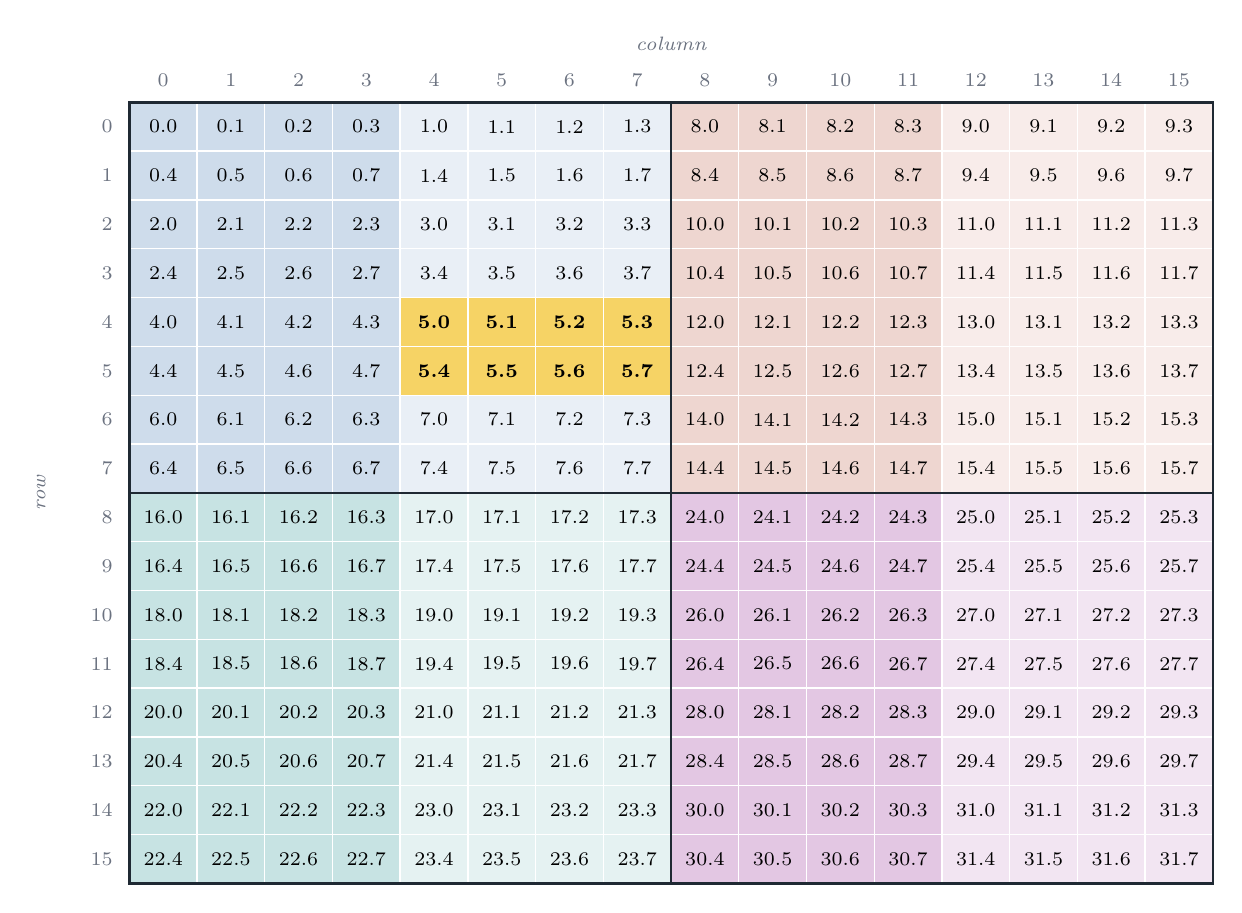
\begin{tikzpicture}[x=8.6mm, y=-6.2mm, font=\scriptsize]
  \node[text=apple] at (0.5,-0.45) {0};
  \node[text=apple] at (1.5,-0.45) {1};
  \node[text=apple] at (2.5,-0.45) {2};
  \node[text=apple] at (3.5,-0.45) {3};
  \node[text=apple] at (4.5,-0.45) {4};
  \node[text=apple] at (5.5,-0.45) {5};
  \node[text=apple] at (6.5,-0.45) {6};
  \node[text=apple] at (7.5,-0.45) {7};
  \node[text=apple] at (8.5,-0.45) {8};
  \node[text=apple] at (9.5,-0.45) {9};
  \node[text=apple] at (10.5,-0.45) {10};
  \node[text=apple] at (11.5,-0.45) {11};
  \node[text=apple] at (12.5,-0.45) {12};
  \node[text=apple] at (13.5,-0.45) {13};
  \node[text=apple] at (14.5,-0.45) {14};
  \node[text=apple] at (15.5,-0.45) {15};
  \node[text=apple, anchor=east] at (-0.1,0.5) {0};
  \node[text=apple, anchor=east] at (-0.1,1.5) {1};
  \node[text=apple, anchor=east] at (-0.1,2.5) {2};
  \node[text=apple, anchor=east] at (-0.1,3.5) {3};
  \node[text=apple, anchor=east] at (-0.1,4.5) {4};
  \node[text=apple, anchor=east] at (-0.1,5.5) {5};
  \node[text=apple, anchor=east] at (-0.1,6.5) {6};
  \node[text=apple, anchor=east] at (-0.1,7.5) {7};
  \node[text=apple, anchor=east] at (-0.1,8.5) {8};
  \node[text=apple, anchor=east] at (-0.1,9.5) {9};
  \node[text=apple, anchor=east] at (-0.1,10.5) {10};
  \node[text=apple, anchor=east] at (-0.1,11.5) {11};
  \node[text=apple, anchor=east] at (-0.1,12.5) {12};
  \node[text=apple, anchor=east] at (-0.1,13.5) {13};
  \node[text=apple, anchor=east] at (-0.1,14.5) {14};
  \node[text=apple, anchor=east] at (-0.1,15.5) {15};
  \fill[ours!22] (0,0) rectangle +(1,1); \node at (0.5,0.5) {0.0};
  \fill[ours!22] (1,0) rectangle +(1,1); \node at (1.5,0.5) {0.1};
  \fill[ours!22] (2,0) rectangle +(1,1); \node at (2.5,0.5) {0.2};
  \fill[ours!22] (3,0) rectangle +(1,1); \node at (3.5,0.5) {0.3};
  \fill[ours!10] (4,0) rectangle +(1,1); \node at (4.5,0.5) {1.0};
  \fill[ours!10] (5,0) rectangle +(1,1); \node at (5.5,0.5) {1.1};
  \fill[ours!10] (6,0) rectangle +(1,1); \node at (6.5,0.5) {1.2};
  \fill[ours!10] (7,0) rectangle +(1,1); \node at (7.5,0.5) {1.3};
  \fill[native!22] (8,0) rectangle +(1,1); \node at (8.5,0.5) {8.0};
  \fill[native!22] (9,0) rectangle +(1,1); \node at (9.5,0.5) {8.1};
  \fill[native!22] (10,0) rectangle +(1,1); \node at (10.5,0.5) {8.2};
  \fill[native!22] (11,0) rectangle +(1,1); \node at (11.5,0.5) {8.3};
  \fill[native!10] (12,0) rectangle +(1,1); \node at (12.5,0.5) {9.0};
  \fill[native!10] (13,0) rectangle +(1,1); \node at (13.5,0.5) {9.1};
  \fill[native!10] (14,0) rectangle +(1,1); \node at (14.5,0.5) {9.2};
  \fill[native!10] (15,0) rectangle +(1,1); \node at (15.5,0.5) {9.3};
  \fill[ours!22] (0,1) rectangle +(1,1); \node at (0.5,1.5) {0.4};
  \fill[ours!22] (1,1) rectangle +(1,1); \node at (1.5,1.5) {0.5};
  \fill[ours!22] (2,1) rectangle +(1,1); \node at (2.5,1.5) {0.6};
  \fill[ours!22] (3,1) rectangle +(1,1); \node at (3.5,1.5) {0.7};
  \fill[ours!10] (4,1) rectangle +(1,1); \node at (4.5,1.5) {1.4};
  \fill[ours!10] (5,1) rectangle +(1,1); \node at (5.5,1.5) {1.5};
  \fill[ours!10] (6,1) rectangle +(1,1); \node at (6.5,1.5) {1.6};
  \fill[ours!10] (7,1) rectangle +(1,1); \node at (7.5,1.5) {1.7};
  \fill[native!22] (8,1) rectangle +(1,1); \node at (8.5,1.5) {8.4};
  \fill[native!22] (9,1) rectangle +(1,1); \node at (9.5,1.5) {8.5};
  \fill[native!22] (10,1) rectangle +(1,1); \node at (10.5,1.5) {8.6};
  \fill[native!22] (11,1) rectangle +(1,1); \node at (11.5,1.5) {8.7};
  \fill[native!10] (12,1) rectangle +(1,1); \node at (12.5,1.5) {9.4};
  \fill[native!10] (13,1) rectangle +(1,1); \node at (13.5,1.5) {9.5};
  \fill[native!10] (14,1) rectangle +(1,1); \node at (14.5,1.5) {9.6};
  \fill[native!10] (15,1) rectangle +(1,1); \node at (15.5,1.5) {9.7};
  \fill[ours!22] (0,2) rectangle +(1,1); \node at (0.5,2.5) {2.0};
  \fill[ours!22] (1,2) rectangle +(1,1); \node at (1.5,2.5) {2.1};
  \fill[ours!22] (2,2) rectangle +(1,1); \node at (2.5,2.5) {2.2};
  \fill[ours!22] (3,2) rectangle +(1,1); \node at (3.5,2.5) {2.3};
  \fill[ours!10] (4,2) rectangle +(1,1); \node at (4.5,2.5) {3.0};
  \fill[ours!10] (5,2) rectangle +(1,1); \node at (5.5,2.5) {3.1};
  \fill[ours!10] (6,2) rectangle +(1,1); \node at (6.5,2.5) {3.2};
  \fill[ours!10] (7,2) rectangle +(1,1); \node at (7.5,2.5) {3.3};
  \fill[native!22] (8,2) rectangle +(1,1); \node at (8.5,2.5) {10.0};
  \fill[native!22] (9,2) rectangle +(1,1); \node at (9.5,2.5) {10.1};
  \fill[native!22] (10,2) rectangle +(1,1); \node at (10.5,2.5) {10.2};
  \fill[native!22] (11,2) rectangle +(1,1); \node at (11.5,2.5) {10.3};
  \fill[native!10] (12,2) rectangle +(1,1); \node at (12.5,2.5) {11.0};
  \fill[native!10] (13,2) rectangle +(1,1); \node at (13.5,2.5) {11.1};
  \fill[native!10] (14,2) rectangle +(1,1); \node at (14.5,2.5) {11.2};
  \fill[native!10] (15,2) rectangle +(1,1); \node at (15.5,2.5) {11.3};
  \fill[ours!22] (0,3) rectangle +(1,1); \node at (0.5,3.5) {2.4};
  \fill[ours!22] (1,3) rectangle +(1,1); \node at (1.5,3.5) {2.5};
  \fill[ours!22] (2,3) rectangle +(1,1); \node at (2.5,3.5) {2.6};
  \fill[ours!22] (3,3) rectangle +(1,1); \node at (3.5,3.5) {2.7};
  \fill[ours!10] (4,3) rectangle +(1,1); \node at (4.5,3.5) {3.4};
  \fill[ours!10] (5,3) rectangle +(1,1); \node at (5.5,3.5) {3.5};
  \fill[ours!10] (6,3) rectangle +(1,1); \node at (6.5,3.5) {3.6};
  \fill[ours!10] (7,3) rectangle +(1,1); \node at (7.5,3.5) {3.7};
  \fill[native!22] (8,3) rectangle +(1,1); \node at (8.5,3.5) {10.4};
  \fill[native!22] (9,3) rectangle +(1,1); \node at (9.5,3.5) {10.5};
  \fill[native!22] (10,3) rectangle +(1,1); \node at (10.5,3.5) {10.6};
  \fill[native!22] (11,3) rectangle +(1,1); \node at (11.5,3.5) {10.7};
  \fill[native!10] (12,3) rectangle +(1,1); \node at (12.5,3.5) {11.4};
  \fill[native!10] (13,3) rectangle +(1,1); \node at (13.5,3.5) {11.5};
  \fill[native!10] (14,3) rectangle +(1,1); \node at (14.5,3.5) {11.6};
  \fill[native!10] (15,3) rectangle +(1,1); \node at (15.5,3.5) {11.7};
  \fill[ours!22] (0,4) rectangle +(1,1); \node at (0.5,4.5) {4.0};
  \fill[ours!22] (1,4) rectangle +(1,1); \node at (1.5,4.5) {4.1};
  \fill[ours!22] (2,4) rectangle +(1,1); \node at (2.5,4.5) {4.2};
  \fill[ours!22] (3,4) rectangle +(1,1); \node at (3.5,4.5) {4.3};
  \fill[hilite] (4,4) rectangle +(1,1); \node at (4.5,4.5) {\textbf{5.0}};
  \fill[hilite] (5,4) rectangle +(1,1); \node at (5.5,4.5) {\textbf{5.1}};
  \fill[hilite] (6,4) rectangle +(1,1); \node at (6.5,4.5) {\textbf{5.2}};
  \fill[hilite] (7,4) rectangle +(1,1); \node at (7.5,4.5) {\textbf{5.3}};
  \fill[native!22] (8,4) rectangle +(1,1); \node at (8.5,4.5) {12.0};
  \fill[native!22] (9,4) rectangle +(1,1); \node at (9.5,4.5) {12.1};
  \fill[native!22] (10,4) rectangle +(1,1); \node at (10.5,4.5) {12.2};
  \fill[native!22] (11,4) rectangle +(1,1); \node at (11.5,4.5) {12.3};
  \fill[native!10] (12,4) rectangle +(1,1); \node at (12.5,4.5) {13.0};
  \fill[native!10] (13,4) rectangle +(1,1); \node at (13.5,4.5) {13.1};
  \fill[native!10] (14,4) rectangle +(1,1); \node at (14.5,4.5) {13.2};
  \fill[native!10] (15,4) rectangle +(1,1); \node at (15.5,4.5) {13.3};
  \fill[ours!22] (0,5) rectangle +(1,1); \node at (0.5,5.5) {4.4};
  \fill[ours!22] (1,5) rectangle +(1,1); \node at (1.5,5.5) {4.5};
  \fill[ours!22] (2,5) rectangle +(1,1); \node at (2.5,5.5) {4.6};
  \fill[ours!22] (3,5) rectangle +(1,1); \node at (3.5,5.5) {4.7};
  \fill[hilite] (4,5) rectangle +(1,1); \node at (4.5,5.5) {\textbf{5.4}};
  \fill[hilite] (5,5) rectangle +(1,1); \node at (5.5,5.5) {\textbf{5.5}};
  \fill[hilite] (6,5) rectangle +(1,1); \node at (6.5,5.5) {\textbf{5.6}};
  \fill[hilite] (7,5) rectangle +(1,1); \node at (7.5,5.5) {\textbf{5.7}};
  \fill[native!22] (8,5) rectangle +(1,1); \node at (8.5,5.5) {12.4};
  \fill[native!22] (9,5) rectangle +(1,1); \node at (9.5,5.5) {12.5};
  \fill[native!22] (10,5) rectangle +(1,1); \node at (10.5,5.5) {12.6};
  \fill[native!22] (11,5) rectangle +(1,1); \node at (11.5,5.5) {12.7};
  \fill[native!10] (12,5) rectangle +(1,1); \node at (12.5,5.5) {13.4};
  \fill[native!10] (13,5) rectangle +(1,1); \node at (13.5,5.5) {13.5};
  \fill[native!10] (14,5) rectangle +(1,1); \node at (14.5,5.5) {13.6};
  \fill[native!10] (15,5) rectangle +(1,1); \node at (15.5,5.5) {13.7};
  \fill[ours!22] (0,6) rectangle +(1,1); \node at (0.5,6.5) {6.0};
  \fill[ours!22] (1,6) rectangle +(1,1); \node at (1.5,6.5) {6.1};
  \fill[ours!22] (2,6) rectangle +(1,1); \node at (2.5,6.5) {6.2};
  \fill[ours!22] (3,6) rectangle +(1,1); \node at (3.5,6.5) {6.3};
  \fill[ours!10] (4,6) rectangle +(1,1); \node at (4.5,6.5) {7.0};
  \fill[ours!10] (5,6) rectangle +(1,1); \node at (5.5,6.5) {7.1};
  \fill[ours!10] (6,6) rectangle +(1,1); \node at (6.5,6.5) {7.2};
  \fill[ours!10] (7,6) rectangle +(1,1); \node at (7.5,6.5) {7.3};
  \fill[native!22] (8,6) rectangle +(1,1); \node at (8.5,6.5) {14.0};
  \fill[native!22] (9,6) rectangle +(1,1); \node at (9.5,6.5) {14.1};
  \fill[native!22] (10,6) rectangle +(1,1); \node at (10.5,6.5) {14.2};
  \fill[native!22] (11,6) rectangle +(1,1); \node at (11.5,6.5) {14.3};
  \fill[native!10] (12,6) rectangle +(1,1); \node at (12.5,6.5) {15.0};
  \fill[native!10] (13,6) rectangle +(1,1); \node at (13.5,6.5) {15.1};
  \fill[native!10] (14,6) rectangle +(1,1); \node at (14.5,6.5) {15.2};
  \fill[native!10] (15,6) rectangle +(1,1); \node at (15.5,6.5) {15.3};
  \fill[ours!22] (0,7) rectangle +(1,1); \node at (0.5,7.5) {6.4};
  \fill[ours!22] (1,7) rectangle +(1,1); \node at (1.5,7.5) {6.5};
  \fill[ours!22] (2,7) rectangle +(1,1); \node at (2.5,7.5) {6.6};
  \fill[ours!22] (3,7) rectangle +(1,1); \node at (3.5,7.5) {6.7};
  \fill[ours!10] (4,7) rectangle +(1,1); \node at (4.5,7.5) {7.4};
  \fill[ours!10] (5,7) rectangle +(1,1); \node at (5.5,7.5) {7.5};
  \fill[ours!10] (6,7) rectangle +(1,1); \node at (6.5,7.5) {7.6};
  \fill[ours!10] (7,7) rectangle +(1,1); \node at (7.5,7.5) {7.7};
  \fill[native!22] (8,7) rectangle +(1,1); \node at (8.5,7.5) {14.4};
  \fill[native!22] (9,7) rectangle +(1,1); \node at (9.5,7.5) {14.5};
  \fill[native!22] (10,7) rectangle +(1,1); \node at (10.5,7.5) {14.6};
  \fill[native!22] (11,7) rectangle +(1,1); \node at (11.5,7.5) {14.7};
  \fill[native!10] (12,7) rectangle +(1,1); \node at (12.5,7.5) {15.4};
  \fill[native!10] (13,7) rectangle +(1,1); \node at (13.5,7.5) {15.5};
  \fill[native!10] (14,7) rectangle +(1,1); \node at (14.5,7.5) {15.6};
  \fill[native!10] (15,7) rectangle +(1,1); \node at (15.5,7.5) {15.7};
  \fill[teal!22] (0,8) rectangle +(1,1); \node at (0.5,8.5) {16.0};
  \fill[teal!22] (1,8) rectangle +(1,1); \node at (1.5,8.5) {16.1};
  \fill[teal!22] (2,8) rectangle +(1,1); \node at (2.5,8.5) {16.2};
  \fill[teal!22] (3,8) rectangle +(1,1); \node at (3.5,8.5) {16.3};
  \fill[teal!10] (4,8) rectangle +(1,1); \node at (4.5,8.5) {17.0};
  \fill[teal!10] (5,8) rectangle +(1,1); \node at (5.5,8.5) {17.1};
  \fill[teal!10] (6,8) rectangle +(1,1); \node at (6.5,8.5) {17.2};
  \fill[teal!10] (7,8) rectangle +(1,1); \node at (7.5,8.5) {17.3};
  \fill[violet!22] (8,8) rectangle +(1,1); \node at (8.5,8.5) {24.0};
  \fill[violet!22] (9,8) rectangle +(1,1); \node at (9.5,8.5) {24.1};
  \fill[violet!22] (10,8) rectangle +(1,1); \node at (10.5,8.5) {24.2};
  \fill[violet!22] (11,8) rectangle +(1,1); \node at (11.5,8.5) {24.3};
  \fill[violet!10] (12,8) rectangle +(1,1); \node at (12.5,8.5) {25.0};
  \fill[violet!10] (13,8) rectangle +(1,1); \node at (13.5,8.5) {25.1};
  \fill[violet!10] (14,8) rectangle +(1,1); \node at (14.5,8.5) {25.2};
  \fill[violet!10] (15,8) rectangle +(1,1); \node at (15.5,8.5) {25.3};
  \fill[teal!22] (0,9) rectangle +(1,1); \node at (0.5,9.5) {16.4};
  \fill[teal!22] (1,9) rectangle +(1,1); \node at (1.5,9.5) {16.5};
  \fill[teal!22] (2,9) rectangle +(1,1); \node at (2.5,9.5) {16.6};
  \fill[teal!22] (3,9) rectangle +(1,1); \node at (3.5,9.5) {16.7};
  \fill[teal!10] (4,9) rectangle +(1,1); \node at (4.5,9.5) {17.4};
  \fill[teal!10] (5,9) rectangle +(1,1); \node at (5.5,9.5) {17.5};
  \fill[teal!10] (6,9) rectangle +(1,1); \node at (6.5,9.5) {17.6};
  \fill[teal!10] (7,9) rectangle +(1,1); \node at (7.5,9.5) {17.7};
  \fill[violet!22] (8,9) rectangle +(1,1); \node at (8.5,9.5) {24.4};
  \fill[violet!22] (9,9) rectangle +(1,1); \node at (9.5,9.5) {24.5};
  \fill[violet!22] (10,9) rectangle +(1,1); \node at (10.5,9.5) {24.6};
  \fill[violet!22] (11,9) rectangle +(1,1); \node at (11.5,9.5) {24.7};
  \fill[violet!10] (12,9) rectangle +(1,1); \node at (12.5,9.5) {25.4};
  \fill[violet!10] (13,9) rectangle +(1,1); \node at (13.5,9.5) {25.5};
  \fill[violet!10] (14,9) rectangle +(1,1); \node at (14.5,9.5) {25.6};
  \fill[violet!10] (15,9) rectangle +(1,1); \node at (15.5,9.5) {25.7};
  \fill[teal!22] (0,10) rectangle +(1,1); \node at (0.5,10.5) {18.0};
  \fill[teal!22] (1,10) rectangle +(1,1); \node at (1.5,10.5) {18.1};
  \fill[teal!22] (2,10) rectangle +(1,1); \node at (2.5,10.5) {18.2};
  \fill[teal!22] (3,10) rectangle +(1,1); \node at (3.5,10.5) {18.3};
  \fill[teal!10] (4,10) rectangle +(1,1); \node at (4.5,10.5) {19.0};
  \fill[teal!10] (5,10) rectangle +(1,1); \node at (5.5,10.5) {19.1};
  \fill[teal!10] (6,10) rectangle +(1,1); \node at (6.5,10.5) {19.2};
  \fill[teal!10] (7,10) rectangle +(1,1); \node at (7.5,10.5) {19.3};
  \fill[violet!22] (8,10) rectangle +(1,1); \node at (8.5,10.5) {26.0};
  \fill[violet!22] (9,10) rectangle +(1,1); \node at (9.5,10.5) {26.1};
  \fill[violet!22] (10,10) rectangle +(1,1); \node at (10.5,10.5) {26.2};
  \fill[violet!22] (11,10) rectangle +(1,1); \node at (11.5,10.5) {26.3};
  \fill[violet!10] (12,10) rectangle +(1,1); \node at (12.5,10.5) {27.0};
  \fill[violet!10] (13,10) rectangle +(1,1); \node at (13.5,10.5) {27.1};
  \fill[violet!10] (14,10) rectangle +(1,1); \node at (14.5,10.5) {27.2};
  \fill[violet!10] (15,10) rectangle +(1,1); \node at (15.5,10.5) {27.3};
  \fill[teal!22] (0,11) rectangle +(1,1); \node at (0.5,11.5) {18.4};
  \fill[teal!22] (1,11) rectangle +(1,1); \node at (1.5,11.5) {18.5};
  \fill[teal!22] (2,11) rectangle +(1,1); \node at (2.5,11.5) {18.6};
  \fill[teal!22] (3,11) rectangle +(1,1); \node at (3.5,11.5) {18.7};
  \fill[teal!10] (4,11) rectangle +(1,1); \node at (4.5,11.5) {19.4};
  \fill[teal!10] (5,11) rectangle +(1,1); \node at (5.5,11.5) {19.5};
  \fill[teal!10] (6,11) rectangle +(1,1); \node at (6.5,11.5) {19.6};
  \fill[teal!10] (7,11) rectangle +(1,1); \node at (7.5,11.5) {19.7};
  \fill[violet!22] (8,11) rectangle +(1,1); \node at (8.5,11.5) {26.4};
  \fill[violet!22] (9,11) rectangle +(1,1); \node at (9.5,11.5) {26.5};
  \fill[violet!22] (10,11) rectangle +(1,1); \node at (10.5,11.5) {26.6};
  \fill[violet!22] (11,11) rectangle +(1,1); \node at (11.5,11.5) {26.7};
  \fill[violet!10] (12,11) rectangle +(1,1); \node at (12.5,11.5) {27.4};
  \fill[violet!10] (13,11) rectangle +(1,1); \node at (13.5,11.5) {27.5};
  \fill[violet!10] (14,11) rectangle +(1,1); \node at (14.5,11.5) {27.6};
  \fill[violet!10] (15,11) rectangle +(1,1); \node at (15.5,11.5) {27.7};
  \fill[teal!22] (0,12) rectangle +(1,1); \node at (0.5,12.5) {20.0};
  \fill[teal!22] (1,12) rectangle +(1,1); \node at (1.5,12.5) {20.1};
  \fill[teal!22] (2,12) rectangle +(1,1); \node at (2.5,12.5) {20.2};
  \fill[teal!22] (3,12) rectangle +(1,1); \node at (3.5,12.5) {20.3};
  \fill[teal!10] (4,12) rectangle +(1,1); \node at (4.5,12.5) {21.0};
  \fill[teal!10] (5,12) rectangle +(1,1); \node at (5.5,12.5) {21.1};
  \fill[teal!10] (6,12) rectangle +(1,1); \node at (6.5,12.5) {21.2};
  \fill[teal!10] (7,12) rectangle +(1,1); \node at (7.5,12.5) {21.3};
  \fill[violet!22] (8,12) rectangle +(1,1); \node at (8.5,12.5) {28.0};
  \fill[violet!22] (9,12) rectangle +(1,1); \node at (9.5,12.5) {28.1};
  \fill[violet!22] (10,12) rectangle +(1,1); \node at (10.5,12.5) {28.2};
  \fill[violet!22] (11,12) rectangle +(1,1); \node at (11.5,12.5) {28.3};
  \fill[violet!10] (12,12) rectangle +(1,1); \node at (12.5,12.5) {29.0};
  \fill[violet!10] (13,12) rectangle +(1,1); \node at (13.5,12.5) {29.1};
  \fill[violet!10] (14,12) rectangle +(1,1); \node at (14.5,12.5) {29.2};
  \fill[violet!10] (15,12) rectangle +(1,1); \node at (15.5,12.5) {29.3};
  \fill[teal!22] (0,13) rectangle +(1,1); \node at (0.5,13.5) {20.4};
  \fill[teal!22] (1,13) rectangle +(1,1); \node at (1.5,13.5) {20.5};
  \fill[teal!22] (2,13) rectangle +(1,1); \node at (2.5,13.5) {20.6};
  \fill[teal!22] (3,13) rectangle +(1,1); \node at (3.5,13.5) {20.7};
  \fill[teal!10] (4,13) rectangle +(1,1); \node at (4.5,13.5) {21.4};
  \fill[teal!10] (5,13) rectangle +(1,1); \node at (5.5,13.5) {21.5};
  \fill[teal!10] (6,13) rectangle +(1,1); \node at (6.5,13.5) {21.6};
  \fill[teal!10] (7,13) rectangle +(1,1); \node at (7.5,13.5) {21.7};
  \fill[violet!22] (8,13) rectangle +(1,1); \node at (8.5,13.5) {28.4};
  \fill[violet!22] (9,13) rectangle +(1,1); \node at (9.5,13.5) {28.5};
  \fill[violet!22] (10,13) rectangle +(1,1); \node at (10.5,13.5) {28.6};
  \fill[violet!22] (11,13) rectangle +(1,1); \node at (11.5,13.5) {28.7};
  \fill[violet!10] (12,13) rectangle +(1,1); \node at (12.5,13.5) {29.4};
  \fill[violet!10] (13,13) rectangle +(1,1); \node at (13.5,13.5) {29.5};
  \fill[violet!10] (14,13) rectangle +(1,1); \node at (14.5,13.5) {29.6};
  \fill[violet!10] (15,13) rectangle +(1,1); \node at (15.5,13.5) {29.7};
  \fill[teal!22] (0,14) rectangle +(1,1); \node at (0.5,14.5) {22.0};
  \fill[teal!22] (1,14) rectangle +(1,1); \node at (1.5,14.5) {22.1};
  \fill[teal!22] (2,14) rectangle +(1,1); \node at (2.5,14.5) {22.2};
  \fill[teal!22] (3,14) rectangle +(1,1); \node at (3.5,14.5) {22.3};
  \fill[teal!10] (4,14) rectangle +(1,1); \node at (4.5,14.5) {23.0};
  \fill[teal!10] (5,14) rectangle +(1,1); \node at (5.5,14.5) {23.1};
  \fill[teal!10] (6,14) rectangle +(1,1); \node at (6.5,14.5) {23.2};
  \fill[teal!10] (7,14) rectangle +(1,1); \node at (7.5,14.5) {23.3};
  \fill[violet!22] (8,14) rectangle +(1,1); \node at (8.5,14.5) {30.0};
  \fill[violet!22] (9,14) rectangle +(1,1); \node at (9.5,14.5) {30.1};
  \fill[violet!22] (10,14) rectangle +(1,1); \node at (10.5,14.5) {30.2};
  \fill[violet!22] (11,14) rectangle +(1,1); \node at (11.5,14.5) {30.3};
  \fill[violet!10] (12,14) rectangle +(1,1); \node at (12.5,14.5) {31.0};
  \fill[violet!10] (13,14) rectangle +(1,1); \node at (13.5,14.5) {31.1};
  \fill[violet!10] (14,14) rectangle +(1,1); \node at (14.5,14.5) {31.2};
  \fill[violet!10] (15,14) rectangle +(1,1); \node at (15.5,14.5) {31.3};
  \fill[teal!22] (0,15) rectangle +(1,1); \node at (0.5,15.5) {22.4};
  \fill[teal!22] (1,15) rectangle +(1,1); \node at (1.5,15.5) {22.5};
  \fill[teal!22] (2,15) rectangle +(1,1); \node at (2.5,15.5) {22.6};
  \fill[teal!22] (3,15) rectangle +(1,1); \node at (3.5,15.5) {22.7};
  \fill[teal!10] (4,15) rectangle +(1,1); \node at (4.5,15.5) {23.4};
  \fill[teal!10] (5,15) rectangle +(1,1); \node at (5.5,15.5) {23.5};
  \fill[teal!10] (6,15) rectangle +(1,1); \node at (6.5,15.5) {23.6};
  \fill[teal!10] (7,15) rectangle +(1,1); \node at (7.5,15.5) {23.7};
  \fill[violet!22] (8,15) rectangle +(1,1); \node at (8.5,15.5) {30.4};
  \fill[violet!22] (9,15) rectangle +(1,1); \node at (9.5,15.5) {30.5};
  \fill[violet!22] (10,15) rectangle +(1,1); \node at (10.5,15.5) {30.6};
  \fill[violet!22] (11,15) rectangle +(1,1); \node at (11.5,15.5) {30.7};
  \fill[violet!10] (12,15) rectangle +(1,1); \node at (12.5,15.5) {31.4};
  \fill[violet!10] (13,15) rectangle +(1,1); \node at (13.5,15.5) {31.5};
  \fill[violet!10] (14,15) rectangle +(1,1); \node at (14.5,15.5) {31.6};
  \fill[violet!10] (15,15) rectangle +(1,1); \node at (15.5,15.5) {31.7};
  \foreach \i in {0,...,16} {\draw[white, line width=0.5pt] (\i,0) -- (\i,16); \draw[white, line width=0.5pt] (0,\i) -- (16,\i);}
  \draw[ink, line width=0.9pt] (0,0) rectangle (16,16) (8,0) -- (8,16) (0,8) -- (16,8);
  \node[text=apple, font=\scriptsize\itshape] at (8,-1.2) {column};
  \node[text=apple, font=\scriptsize\itshape, rotate=90] at (-1.3,8) {row};
\end{tikzpicture}
\caption{Lane and element slot of each element of a 16 × 16 A or D tile. Each cell is \emph{lane.slot}: the lane that holds the
element and which of its eight element slots it occupies (a half A fragment packs the eight slots into four registers,
an fp32 D into eight). The coordinates are the instruction's own (canonical), before any packing convention
(\cref{sec:coordinate-systems}). The four quadrants are the four groups of eight
lanes (blue, red, teal, violet: lanes 0–7, 8–15, 16–23 and 24–31); alternate lanes are shaded darker and
lighter to mark each lane's 2 × 4 block. Lane 5, the lane followed in \cref{sec:one-program-ir}, is
highlighted; this compiler's B-row packing stores those elements at application rows 2 and 10. The map was measured with one-hot probes over 6,651 dispatches (MM~\mm{3}); the figure is generated
from the inverse formula of \cref{sec:fragment-layouts}.}
\label{fig:fragment-map}
\end{figure}


A lane's four slots in a row are consecutive columns, so one 8-byte access per row loads them.

\begin{xltabular}{\linewidth}{@{}lllX@{}}
\caption{A/D fragment map by lane quadrant (MM~\mm{0.5}).}\label{tab:lane-quadrants}\\
\toprule
Lanes & Rows & Columns & Within the eight-lane group, local lane q \\
\midrule
\endfirsthead
\tablecontinued{4}
\toprule
Lanes & Rows & Columns & Within the eight-lane group, local lane q \\
\midrule
\endhead
0–7 & 0–7 & 0–7 & rows \code{2*(q>>1)} and \code{+1}, columns \code{4*(q\&1)} to \code{+3} \\*
8–15 & 0–7 & 8–15 & same, column base +8 \\*
16–23 & 8–15 & 0–7 & same, row base +8 \\*
24–31 & 8–15 & 8–15 & same, both bases +8 \\*
\bottomrule
\end{xltabular}

A packer needs the inverse maps, each returning (lane, slot). Both are bijections onto the 256 positions
(re-verified, MM~\mm{3}):

\begin{lstlisting}
pos(r, c)   = (16*(r>>3) + 8*(c>>3) + 2*((r>>1)&3) + ((c>>2)&1),   4*(r&1) + (c&3))      A and D
pos_b(k, c) = (16*((k>>2)&1) + 8*(c>>3) + 2*(k&3) + ((c>>2)&1),     4*(k>>3) + (c&3))      B
\end{lstlisting}

\begin{longtable}{@{}rllll@{}}
\caption{A/D and B fragment contents of four sample lanes, derived from the layout formulas.}\label{tab:fragment-examples}\\
\toprule
Lane & A/D: slots 0–3 & A/D: slots 4–7 & B: slots 0–3 & B: slots 4–7 \\
\midrule
\endfirsthead
\tablecontinued{5}
\toprule
Lane & A/D: slots 0–3 & A/D: slots 4–7 & B: slots 0–3 & B: slots 4–7 \\
\midrule
\endhead
0 & D(0, 0..3) & D(1, 0..3) & B(0, 0..3) & B(8, 0..3) \\
9 & D(0, 12..15) & D(1, 12..15) & B(0, 12..15) & B(8, 12..15) \\
17 & D(8, 4..7) & D(9, 4..7) & B(4, 4..7) & B(12, 4..7) \\
22 & D(14, 0..3) & D(15, 0..3) & B(7, 0..3) & B(15, 0..3) \\
\bottomrule
\end{longtable}

Lane 22 step by step: \code{l>>4 = 1}, \code{(l>>1)\&3 = 11\&3 = 3}, \code{(l>>3)\&1 = 0}, \code{l\&1 = 0}. For A/D, \code{row = 8 + 6 + (j>>2)}
and \code{col = 0 + 0 + (j\&3)}, so slot 6 is D(15, 2). Inverse: \code{pos(15, 2) = (16*1 + 8*0 + 2*(7\&3) + ((2>>2)\&1), 4*(15\&1) + 2) = (22, 6)}. For B, \code{k = 4 + 3 + 8*(j>>2)}, so slot 6 is B(15, 2), and \code{pos\_b(15, 2) = (16*1 + 0 + 2*3 + 0, 4*1 + 2) = (22, 6)}. With transA = 1, lane 22 slot j holds A(row \code{2*(j\&3)}, k \code{7 + 8*(j>>2)}): slot 6 is
A(4, 15).

The B map is the A/D map with rows rotated by one bit, \code{pos\_b(k, c) = pos(rotl1(k), c)}, at 256 of 256
positions (measured, re-verified, MM~\mm{3}). Check on lane 22: \code{rotl1(7) = 14} and \code{pos(14, 2) = (22, 2) = pos\_b(7, 2)}.

The 16-bit MMA, \op{5106}, its no-C sibling and the fp32 × fp32 MMA, \op{5098}, use the same destination layout.
Destinations measured in different kernels can still differ by \code{rotl1} on the row index at all 256 positions, the
same rotation Apple's cooperative-tensor coordinates carry (MM~\mm{3}, MM~\mm{19}). \Cref{sec:coordinate-systems}
traces this to the producing kernel's row labelling, which also accounts for the feed-mode relabellings of
\cref{sec:chaining-feed-modes}.

For other operand types (measured, MM~\mm{3}, MM~\mm{19}):

\begin{itemize}
\item fp32 and int8 operands use the same A, B and D maps as half.
\item In Apple-compiled multi-tile destinations, \op{10384} is among 23 forms whose destination is \code{pos\_b} inside
  every 16 × 16 tile with row-major tile blocks, matching at 1,024 of 1,024 (lane, slot) positions (MM~\mm{3}).
\item In the fp32 × fp32 MMA the fp32 A operand and the fp32 D/C share one layout (\code{A\_row == D\_row}, \code{A\_k == D\_col}, 256 of 256), so a D
  can feed the next A with no store and no permutation (MM~\mm{19}).
\item Apple's cooperative-tensor coordinates for a 16 × 16 single-simdgroup destination equal the B map with index 0 as
  column and index 1 as row; relative to the D map, rows are rotated by \code{y = ((r\&7)<<1) | (r>>3)} (Apple's compiler,
  MM~\mm{3}).
\end{itemize}

\begin{xltabular}{\linewidth}{@{}>{\hsize=1.39\hsize}X>{\hsize=0.63\hsize}XlX@{}}
\caption{Register widths and legal bases of tensor operands (measured, MM~\mm{0.7}, MM~\mm{0.1}).}\label{tab:fragment-registers}\\
\toprule
Value & Registers per lane & Alignment & Highest base \\
\midrule
\endfirsthead
\tablecontinued{4}
\toprule
Value & Registers per lane & Alignment & Highest base \\
\midrule
\endhead
scalar & 1 & 1 & R125 \\*
int8 or uint8 fragment & 2 & 2 & R124 \\*
half or bfloat fragment & 4 & 4 & R120 \\*
fp32 A or B fragment & 8 & 8 & R112 \\*
fp32 or int32 accumulator & 8 & 8 & R112 (15 groups: R0, R8, \dots{}, R112) \\*
\bottomrule
\end{xltabular}

R120–R127 cannot hold an 8-register group, because any instruction naming R126 or above is squashed whole
(\cref{sec:namespace}). MM~\mm{0.7} describes the int8 pair as "four byte elements per lane packed across the pair"; how the eight byte
elements of a lane are ordered within the pair is not recorded (open).

Apple's library computes, once
per kernel, the index register \code{R32 = m(l)*128 + col(l)} with \code{m(l) = 4*(l>>4) + ((l>>1)\&3)} and
\code{col(l) = 8*((l>>3)\&1) + 4*(l\&1)}: element (m, col) of a row-major tile at leading dimension 128. Its loads read
\code{[R32*2 + disp]} with displacements \{0, 2048, 32, 4096, 6144\} (2048 steps eight rows, 32 steps sixteen columns). Because
each access moves an 8-row by 16-column sub-tile, rows r and r+8 sit in the two slot halves (Apple's compiler emits,
MM~\mm{7}). No hardware transposition is involved (MM~\mm{19}).

\textbf{Evidence.} MM~\mm{0.5}, MM~\mm{0.7}, MM~\mm{0.14}, MM~\mm{3}, MM~\mm{7}, MM~\mm{19}.

\section{Coordinate systems and packing}\label{sec:coordinate-systems}

\begin{enumerate}
\item \emph{Canonical instruction coordinates}: the map from (lane, slot) to a matrix position that the MMA itself
  uses, \code{pos} for A and D and \code{pos\_b} for B (\cref{sec:fragment-layouts}). The MMA computes D = A B + C in
  these coordinates.
\item \emph{A kernel's packing convention}: which memory element its loads place in each (lane, slot), and where its stores
  write each slot, as set by the kernel's address arithmetic.
\item \emph{Application coordinates}: element (i, j) of the row-major matrix in memory.
\end{enumerate}

Apple-compiled \code{simdgroup\_matrix} code uses \emph{canonical packing}: A, B and D are packed canonically, so an
application row of A or D is the same canonical row. The chaining relabellings were measured on such kernels
(MM~\mm{3}, MM~\mm{13}).

This compiler uses \emph{B-row packing} for every tile, A, B and the C/D tile it loads and stores: lane l, slot j holds
application row \code{m(l) + 8*(j>>2)} and column \code{col(l) + (j\&3)}, with \code{m(l) = 4*(l>>4) + ((l>>1)\&3)} and
\code{col(l) = (l\&8) + 4*(l\&1)} (\code{agxforge/g17/indexgen.py}; \code{agxforge/g17/tlower.py}: "A rows m and m+8 of the tile, B rows k
and k+8", stores "rows m and m+8"). This is the B map applied to every tile. Apple's tensor-ops library computes the same
per-lane index for its tensor loads, and Apple-compiled multi-tile destinations read as \code{pos\_b}
(\cref{sec:fragment-layouts}; MM~\mm{3}, MM~\mm{7}).

For B the two conventions agree. For A and D they differ by a one-bit rotation of the row index: because
\code{pos\_b(r, c) = pos(rotl1(r), c)}, this compiler puts application row r of A in canonical row \code{rotl1(r)}.
Rows of A are the free M index, so canonical row \code{rotl1(r)} of D holds application row r of
the product, and the store, which uses the same convention, writes canonical row \code{rotl1(r)} back to application row
r. Neither the columns nor the K index are permuted, so the reduction over K runs in canonical order and the result is
the one the arithmetic rule of \cref{sec:arithmetic-semantics-supported} predicts in application coordinates.

\textbf{Lane 5 of the running example.} In canonical coordinates its first MMA's D holds elements (4, 4)–(4, 7) in
slots 0–3 and (5, 4)–(5, 7) in slots 4–7 (\cref{fig:fragment-map}). This compiler computes \code{m(5) = 2} and
\code{col(5) = 4}, so its store writes slots 0–3 to application row 2 and slots 4–7 to row 10, columns 4–7. The two
descriptions name the same registers: \code{rotl1(2) = 4} and \code{rotl1(10) = 5}.

When D is fed as B, the next MMA receives D's registers unchanged as its B operand. It reads lane l, slot j as canonical B row \code{k = 4*(l>>4) + ((l>>1)\&3) + 8*(j>>2)}, and
that register holds canonical D row \code{rotl1(k)}.

\begin{itemize}
\item Under B-row packing (this compiler), canonical D row \code{rotl1(k)} is application row k of the product, so the
  consumer reads \code{B\_eff[k][c] = D[k][c]}.
\item Under canonical packing, canonical D row \code{rotl1(k)} is application row \code{rotl1(k)}, so the consumer reads
  \code{B\_eff[k][c] = D[rotl1(k)][c]}: the row-rotated operand that \cref{sec:chaining-feed-modes} measures, which the other
  operand's K index must then be permuted to undo.
\end{itemize}

\Cref{tab:coordinate-example} follows three slots through both conventions. For lane 0, slot 4, canonical D row 1 is
read as B row 8; this compiler's producer placed application row \code{m(0) + 8 = 8} of D in that slot, so the consumer
receives D row 8 as B row 8. With canonical packing the same register carries D row 1, and \code{rotl1(8) = 1}. A D fed
as A needs no relabelling in either convention, because the consumer's A is packed the way the producer packed D.

\begin{longtable}{@{}lllll@{}}
\caption{Three slots in canonical coordinates and in the two packing conventions, for a D tile fed as the next B.}\label{tab:coordinate-example}\\
\toprule
Lane, slot & Canonical D & Read as B & D row, B-row packing & D row, canonical packing \\
\midrule
\endfirsthead
\tablecontinued{5}
\toprule
Lane, slot & Canonical D & Read as B & D row, B-row packing & D row, canonical packing \\
\midrule
\endhead
0, 4 & (1, 0) & (8, 0) & 8 & 1 \\*
5, 0 & (4, 4) & (2, 4) & 2 & 4 \\*
5, 4 & (5, 4) & (10, 4) & 10 & 5 \\*
\bottomrule
\end{longtable}

The feed measurements for both packings agree with this derivation (\cref{sec:chaining-feed-modes}; MM~\mm{13},
MM~\mm{25.103}).

\textbf{Evidence.} MM~\mm{3}, MM~\mm{7}, MM~\mm{13}, MM~\mm{25.103}.

\section{Arithmetic by input type}\label{sec:arithmetic-semantics-supported}

\textbf{Half inputs, fp32 accumulator.} Fitted on half × half inputs, the rule below reproduces 1,680 of 1,680
eps-triples and every other stimulus (measured, MM~\mm{4}, MM~\mm{0.6}). For one output element, with \code{k} the
A-column index of \cref{sec:fragment-layouts}:

\begin{lstlisting}
p_i = RNE32(a[2i]*b[2i] + a[2i+1]*b[2i+1])      i = 0..7    adjacent pairs; products exact
q_j = RNE32(p_j + p_(j+4))                       j = 0..3    pairs eight apart
acc = C
acc = RNE32(acc + q_0); acc = RNE32(acc + q_1); acc = RNE32(acc + q_2); acc = RNE32(acc + q_3)
D   = acc
\end{lstlisting}

% fig:reduction-tree: the measured reduction order of one output element of a 16x16x16 MMA
% (MM 4, MM 0.6). Every node rounds to nearest-even fp32.
\begin{figure}[htbp]
\centering
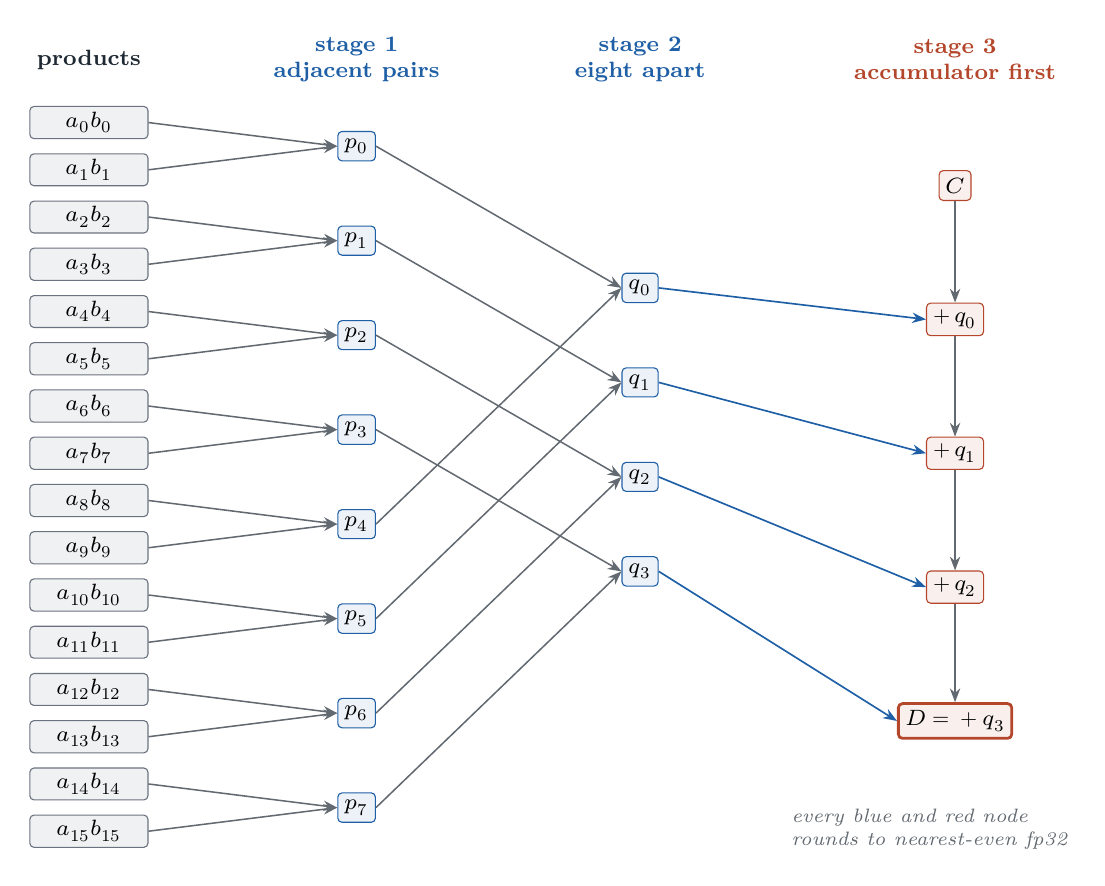
\begin{tikzpicture}[x=1mm, y=-1mm, font=\footnotesize,
    prod/.style={draw=apple, fill=apple!10, rounded corners=1.5pt, inner sep=2pt, minimum width=15mm},
    add/.style={draw=ours, fill=ours!8, rounded corners=1.5pt, inner sep=2.5pt, align=center},
    acc/.style={draw=native, fill=native!8, rounded corners=1.5pt, inner sep=2.5pt, align=center},
    e/.style={->, line width=0.55pt, color=ink!70}]
  % stage headings
  \node[font=\footnotesize\bfseries, text=ink] at (8,-8) {products};
  \node[font=\footnotesize\bfseries, text=ours, align=center] at (42,-8) {stage 1\\adjacent pairs};
  \node[font=\footnotesize\bfseries, text=ours, align=center] at (78,-8) {stage 2\\eight apart};
  \node[font=\footnotesize\bfseries, text=native, align=center] at (118,-8) {stage 3\\accumulator first};
  % sixteen exact products, two per stage-1 node
  \foreach \i in {0,...,15} {
    \pgfmathtruncatemacro\k{\i}
    \node[prod] (x\i) at (8, 6*\i) {$a_{\k} b_{\k}$};
  }
  % stage 1: p_i = RNE(a_{2i}b_{2i} + a_{2i+1}b_{2i+1})
  \foreach \i in {0,...,7} {
    \pgfmathtruncatemacro\a{2*\i}\pgfmathtruncatemacro\b{2*\i+1}
    \node[add] (p\i) at (42, 12*\i+3) {$p_{\i}$};
    \draw[e] (x\a.east) -- (p\i.west);
    \draw[e] (x\b.east) -- (p\i.west);
  }
  % stage 2: q_i = RNE(p_i + p_{i+4})
  \foreach \i in {0,...,3} {
    \pgfmathtruncatemacro\j{\i+4}
    \node[add] (q\i) at (78, 12*\i+21) {$q_{\i}$};
    \draw[e] (p\i.east) -- (q\i.west);
    \draw[e] (p\j.east) -- (q\i.west);
  }
  % stage 3: C enters first, then q0..q3 in a chain
  \node[acc] (C) at (118, 8) {$C$};
  \node[acc] (s0) at (118, 25) {$+\,q_0$};
  \node[acc] (s1) at (118, 42) {$+\,q_1$};
  \node[acc] (s2) at (118, 59) {$+\,q_2$};
  \node[acc, line width=1pt] (D) at (118, 76) {$D = {}+q_3$};
  \draw[e] (C) -- (s0);
  \draw[e] (s0) -- (s1); \draw[e] (s1) -- (s2); \draw[e] (s2) -- (D);
  \foreach \i/\s in {0/s0, 1/s1, 2/s2, 3/D} \draw[e, ours] (q\i.east) -- (\s.west);
  % rounding note
  \node[font=\scriptsize\itshape, text=ink!70, align=left, anchor=north west] at (96, 86)
    {every blue and red node\\rounds to nearest-even fp32};
\end{tikzpicture}
\caption{The measured reduction of one output element. One 16 × 16 × 16 MMA computes each output element from
sixteen exact products. Stage 1 adds adjacent products, $p_i = \mathrm{RNE}_{32}(a_{2i}b_{2i} + a_{2i+1}b_{2i+1})$;
stage 2 adds partial sums eight products apart, $q_i = \mathrm{RNE}_{32}(p_i + p_{i+4})$; stage 3 starts from the
accumulator $C$ and adds $q_0, \dots, q_3$ in order, rounding at every step. The from-zero form, \op{5107}, has no
$C$ and starts the chain from $q_0$. The diagram shows data dependence and makes no claim about the physical
adders (MM~\mm{4}, MM~\mm{0.6}).}
\label{fig:reduction-tree}
\end{figure}


The first stage (\cref{fig:reduction-tree}) adds adjacent products, so \code{(-0) * 1}, with every
other product zero, gives \code{+0}: the pair stage adds a neighbouring \code{+0} first under RNE, and a model with
\code{(-0) + (-0) = -0} mispredicts (measured, MM~\mm{5}). The second stage pairs partial sums eight apart. The
accumulator then enters before the four partial sums, within one issue. The from-zero form, \op{5107}, follows the same tree without C and starts the chain from q0 ("starts from the first reduced
group rather than an encoded zero tuple", MM~\mm{0.3}).

The candidates for the tree were a sequential chain, a balanced tree over the natural K order, a
balanced tree over K interleaved by eight and an exactly rounded sum, and, for the accumulator, adding C first or last.
They differ only in the order of additions and where rounding happens, so the stimuli were placed on single output elements
with half inputs, whose products are always exact in fp32 (an 11-bit by 11-bit significand product fits in 24 bits, and
every such product lies between $2^{-48}$ and about $4.3 \times 10^{9}$, inside fp32's normal range). The main probe was the \textbf{eps-triple}: one product
equal to 1 at a K position i and products equal to a small eps at two other positions j and k, over every placement
(16 × 105 = 1,680 stimuli). Whether the two eps terms are added to each other before either meets the 1 changes the
rounded result, so each triple answers one question about the tree's shape (MM~\mm{4}).

\begin{itemize}
\item Rival fits on the 1,680 triples: balanced tree on natural order 976, interleave-by-8 balanced tree 1,392, the rule
  above 1,680. The triples fixed the pair and interleave stages.
\item Round-to-nearest-even applies at every intermediate; round-toward-zero is rejected on every stimulus.
\item Over a whole tile the rule is exact on 5,120 of 5,120 elements; sequential scores 2,493, balanced 2,764 and
  the exact sum rounded once 2,742 (MM~\mm{4}).
\end{itemize}

\textbf{C before the partial sums.} Let eps = $2^{-24}$, half an fp32 ulp at 1.0. Take C = 1.0 and choose products so that the first two
quad sums are q\_0 = q\_1 = 3 eps and q\_2 = q\_3 = 0 (for example products eps at K positions 0, 1 and 8 give
p\_0 = 2 eps, p\_4 = eps, so q\_0 = 3 eps exactly; positions 2, 3 and 10 do the same for q\_1; eps = $2^{-12} \times 2^{-12}$, both
normal half values).

\begin{lstlisting}
C first (the measured rule):
  acc = RNE32(1 + 3 eps)       = 1 + 4 eps     1.5 ulp is a tie; RNE picks the even neighbour, 2 ulp
  acc = RNE32(1 + 4 eps + 3 eps) = 1 + 8 eps   3.5 ulp is a tie; RNE picks the even neighbour, 4 ulp
C last (any order that sums the q terms first):
  q_0 + q_1 = 6 eps exactly;  RNE32(1 + 6 eps) = 1 + 6 eps   3 ulp, representable
\end{lstlisting}

The hardware returns \code{1 + 8 eps} on the discriminating stimuli (measured, MM~\mm{4}), which rules out every
model that adds C at the end, including an exactly rounded sum.

The repository's bit-exact model \code{tools/tensorops-model/tensorops\_model.py}, which was not used to fit the rule, reproduces Apple's 32 × 32 × 64 library kernel on 6,144 of 6,144
elements (exact-sum-rounded-once: 1,948) and a previously failed tile on 1,024 of 1,024; Apple's \code{matmul2d} is
bit-exact to it on all eight shapes of the speed comparison (measured, MM~\mm{4}, MM~\mm{25.98}). A reference that
adds C after the products is wrong: this compiler's \code{multigemm} class, checked against one, failed its exact check
on 417 of 1,024 elements (MM~\mm{25.89}).

The library's accumulate mode orders C the other way (measured,
MM~\mm{4}, MM~\mm{0.6}, MM~\mm{15}). With a nonzero C, \code{matmul2d}'s
multiply-accumulate mode runs the MMA chain from zero and then loads C and adds it with ordinary fp32 adds (product
first, C last), one extra rounding compared with putting C in the first MMA. Inside one issue C still enters first, so a reference
that models \code{matmul2d} needs both orders.

\textbf{Longer K.} Issues compose through the rounded fp32 accumulator: two-issue chains
reproduce the rule applied twice on 17 of 17 stimuli, three-issue chains 17 of 17; an unrounded inter-issue
accumulator is rejected (8 of 17, 12 of 17). K order is ascending in memory whether the library unrolls or loops: for
K=64, chunk orders 3210, 0213 and 1032 are each rejected by at least one stimulus; a K=128 runtime loop gives
\code{1 + 6 eps} on seven asymmetric probes where descending gives \code{1 + 8 eps} (measured, MM~\mm{4}).

\textbf{Other input types.} The machine model states that bfloat and truncated-fp32
operands follow the same tree (MM~\mm{0.6}, MM~\mm{5}), but the discriminating fit above was made on half inputs only.
Their products are exact only while fp32 can hold them, and unlike half products they can leave fp32's range. Only
single points at the extremes are recorded. A bfloat product at $2^{-133}$ or $2^{-140}$ (fp32 subnormals) is
kept, a bfloat product of 3e38 × 3e38 gives Inf, a truncated-fp32 product $2^{100} \times 2^{-100}$ is exactly 1, and
truncated-fp32 subnormal operands keep their surviving bits (MM~\mm{5}).

\textbf{fp32 operands.} An fp32 A or B has the low 13 bits of its raw pattern cleared, keeping sign, 8 exponent bits
and 10 fraction bits, for normals and subnormals alike (TF32-shaped truncation toward zero; measured, MM~\mm{5}). \code{1 + 2\textasciicircum{}-10 + 2\textasciicircum{}-11} becomes \code{1 + 2\textasciicircum{}-10}; \code{2 - 2\textasciicircum{}-23} becomes \code{2 - 2\textasciicircum{}-10}; the full exponent
range survives (\code{2\textasciicircum{}100 * 2\textasciicircum{}-100 = 1} exactly). The truncated operands then follow the same tree. The fp32-operand forms
cost no issue rate over the half forms (measured, MM~\mm{8}; \cref{ch:performance}).

\textbf{Subnormals.} In the recorded cases nothing in the half or bfloat path or the accumulator flushes (measured,
MM~\mm{5}): half
\code{2\textasciicircum{}-24 * 1} gives \code{2\textasciicircum{}-24}; a bfloat product at \code{2\textasciicircum{}-140} is kept; an fp32 accumulator subnormal passes through. fp32
ALU operations flush subnormal inputs and results (MM~\mm{5}, MM~\mm{17} rule 22; \cref{ch:scalar-arithmetic}), so a subnormal
the MMA produces is flushed to zero by the next fp32 ALU instruction that reads it.

\textbf{Special values.} The record holds 51 edge cases with NaN, Inf or overflowing values (measured, MM~\mm{5}).

\begin{itemize}
\item NaN × 1, NaN × 0, Inf × 0, Inf + (−Inf) inside the sum, and a NaN in C each yield the fp32 quiet NaN \code{0x7fc00000}; Inf × 1 yields Inf; a bfloat product past
  fp32's maximum (3e38 × 3e38) yields Inf; C = fp32 max plus 1 stays fp32 max.
\item half \code{65504 * 65504 = 4.29e9} exactly, and sixteen such products sum exactly.
\item A NaN in an A column poisons the result even where the matching B row is zero, so K padding must be zeros
  (MM~\mm{17} rule 14).
\item Whether Inf − Inf gives the canonical NaN at every position of the tree, and which NaN payloads survive, is not
  recorded beyond these cases (open).
\end{itemize}

\textbf{int8 inputs, int32 accumulator.} Products are exact, with signedness selected independently for A and B
(measured, MM~\mm{5}, MM~\mm{11}). The default form accumulates modulo $2^{32}$ with no saturation, including inside one MMA:
\code{C + 2\textasciicircum{}31} gives \code{-2\textasciicircum{}31}, and \code{16*127*127 + INT\_MAX} wraps to −2147225585. 608 accumulators were exact modulo $2^{32}$ out
to a million iterations in all four sign combinations, 429 of them after leaving the int32 range. One K=16 tile cannot
overflow on its own (16 × 16,384 = 262,144).

\textbf{Saturating int8.} One MMA computes \code{D = clip(C + A.B, -2\textasciicircum{}31, 2\textasciicircum{}31 - 1)}: one signed clip of the exact sixteen-term sum, also for
unsigned operands, which saturate at the signed limit. The rule scored 2,400 of 2,400 tiles in every sign
combination; wrapping scored 1,746, 1,759, 1,742 and 2,129, staged saturation 1,975, 1,886, 1,897 and 2,400. The
unsigned-by-unsigned column (the last) cannot discriminate, because every product is non-negative; the signed cases
carry the result (measured, MM~\mm{11}). An accumulator driven to the limit leaves it again under opposing products.

\begin{itemize}
\item Under transpose, with D seeded to \code{INT32\_MAX - 32} and all-ones int8 operands (exact sum 2147483679), wrap
  predicts −2147483617 and saturation 2147483647. With A transposed, Apple's bytes (byte8 0x44) give −2147483617 on all
  1,024 outputs; with byte8 bit 4 set on all sixteen \op{10384} instances (0x54), 2147483647 on all 1,024; an in-range sum
  (64) is unchanged by the bit (MM~\mm{25.42}). The untransposed pair (0x40, 0x50) behaves the same.
\item A chain of saturating MMAs clips once per issue: on inputs near both rails, wrap, clip after every
  product, clip after every issue and clip once at the end differ pairwise on 21 to 56 of 1,024 elements, and the
  hardware matched clip-per-issue (MM~\mm{25.89}).
\item MM~\mm{20} records saturation at high register numbers as not run.
\end{itemize}

\textbf{Destination conversions.} A kernel narrows the fp32 accumulator with ordinary conversion instructions, which
are not part of the MMA. fp32 to half is IEEE round-to-nearest-even (\code{65520} goes to infinity,
\code{2\textasciicircum{}-25} to zero), and fp32 to bfloat is RNE except for subnormal inputs; the measured rules are in
\cref{tab:conversions} (measured, MM~\mm{5}, MM~\mm{6}, MM~\mm{0.6}, MM~\mm{17} rule 21).

\textbf{16-bit destinations across calls.} A 16-bit destination rounds after every accumulating library call
(measured, MM~\mm{12}, MM~\mm{17} rule 18): four contributions to a half destination give 2054 where one rounding gives
2052; the same contributions inside one call with K=64 give 2052, because internal K slices stay fp32. Use a float
destination across calls.

\textbf{Evidence.} MM~\mm{0.6}, MM~\mm{4}, MM~\mm{5}, MM~\mm{6}, MM~\mm{11}, MM~\mm{12}, MM~\mm{15}, MM~\mm{17}, MM~\mm{19}, MM~\mm{25.42}, MM~\mm{25.89}, MM~\mm{25.98}.

\section{Ordering and the tensor enable}\label{sec:ordering-enable}

\subsection*{Ordering}

\begin{itemize}
\item A tensor MMA carries an 8-bit wait mask at flags bits 24–31, on the scoreboard of \cref{sec:scoreboard}: for a load
  filling slot \code{s}, the consuming MMA must set bit \code{24 + s} (measured, MM~\mm{6}, MM~\mm{0.8}). The bits are
  physically scattered (slot 7 is byte0{[}3{]}; the field carriers are in \cref{sec:scoreboard-publish-wait}). In the
  running example (\cref{sec:one-program-ir}) all eight tile loads fill slot 0 and each MMA's flags word is
  0x01000000, bit 24.
\item In Apple's code each compiled MMA waits on exactly its own load group, so the bits look one-hot (MM~\mm{6}).
  Whether each consumer sets the bit for its producer's slot can be checked from the decoded bytes alone.
\item The tensor load names the slot it fills in operand 1 bits 20–23, as slot + 1, a different carrier from the ordinary
  \op{12709} (measured, MM~\mm{6}, MM~\mm{25.4/R6}; \cref{sec:scoreboard-publish-wait}).
\item On the result side, an ALU instruction placed directly after an MMA, with no wait, read the MMA's result correctly;
  whether the hardware interlocks MMA-to-ALU or the consuming form waits implicitly is open (MM~\mm{6}, MM~\mm{25.90}). In
  this compiler's kernels an ALU read right after the last MMA needed no extra wait and was bit-exact (this compiler, measured,
  MM~\mm{25.105.1}).
\item Feeding D as the next MMA's C, A or B in the same simdgroup needs no wait in the measured forms
  (\cref{sec:chaining-feed-modes}; measured, MM~\mm{0.9}, MM~\mm{13}).
\item Two apparent MMA hazards (a stored result feeding a register-resident consumer; independent back-to-back MMAs)
  came from the host harness's \code{dim} parameter, which bounds how many output bytes are complete
  and host-visible on return; both kernels pass when it covers the output (\code{dim\textasciicircum{}2 * esz}) (MM~\mm{19}, MM~\mm{17} rule 5).
\end{itemize}

\subsection*{The tensor enable (metadata slot 44)}

A kernel that uses the tensor unit carries an enable word in per-kernel metadata slot 44 (format in
\cref{ch:kernel-metadata-image}). Its effect was measured by patching 14 pipelines (MM~\mm{6}, MM~\mm{0.1}).

\begin{itemize}
\item Slot 44 is present exactly when the code contains a tensor MMA: in all 50 such kernels and in no legacy-engine
  kernel.
\item If its low byte is zero, every tensor MMA produces zeros, the pipeline still builds and the dispatch completes
  without error. In the tested patches any nonzero low byte, with the other three bytes arbitrary, is bit-identical
  to the original, so the low byte acts as an on/off switch.
\item A disabled unit produces zeros quickly and neither faults nor stalls: a 1,400-MMA chain runs in 14.75~µs
  instead of 32.0 (8.4~ns per issue instead of 22), a saturated dispatch in 0.587~ms instead of 22.7 (a factor of 39).
  The MMAs still issue, at roughly ALU cost, while writing zeros. The timing fits a power or clock gate better than a
  validity check; the mechanism itself was not measured.
\item With an explicit imageblock in the same kernel, per-kernel slot 19 sits at 55 and the tensor enable moves to slot 54;
  the slot-29 vector is {[}48, 49, 52{]} (Apple's compiler emits, MM~\mm{25.89}). "Slot 44" is its position in the
  tensor-only layout.
\end{itemize}

Each patch was dispatched from a process other than the one that built the archive, with a positive control that
shows a predictable bit moving the output, since Metal caches pipelines (\cref{sec:object-library-archive}; measured,
MM~\mm{17} rule 36, MM~\mm{25.42}).

\textbf{Evidence.} MM~\mm{0.1}, MM~\mm{0.8}, MM~\mm{6}, MM~\mm{13}, MM~\mm{17}, MM~\mm{20}, MM~\mm{25.4/R6}, MM~\mm{25.42}, MM~\mm{25.89},
MM~\mm{25.90}, MM~\mm{25.105.1}.

\section{Tensor loads and stores}\label{sec:tensor-memory-path}

The tensor unit has no memory port of its own; its fragments are filled and drained by the load and store forms of
\cref{tab:tensor-load-store}, which use the addressing of \cref{ch:memory} (measured, MM~\mm{0.8}, MM~\mm{7}).

\begin{xltabular}{\linewidth}{@{}XXX@{}}
\caption{Tensor load and store forms.}\label{tab:tensor-load-store}\\
\toprule
Form & Per-lane payload & Mask \\
\midrule
\endfirsthead
\tablecontinued{3}
\toprule
Form & Per-lane payload & Mask \\
\midrule
\endhead
\op{12674} & two 32-bit words, four 16-bit elements; 12- or 16-byte encoding & immediate (15 or 0) \\*
\op{12675} & two words & 16-bit register \\*
\op{12656} & one word, four int8 elements, byte-addressed & immediate \\*
\op{12657} & one word & 16-bit register \\*
\op{12692} & fp32 elements (element width 4) & not stated in the sources \\*
\op{17257} & four 32-bit words & immediate \\*
\op{17258} & four words & 16-bit register: bit j enables word j (j = 0..3); bits above 3 ignored;
unwritten words keep their prior contents \\*
\bottomrule
\end{xltabular}

An int8 operand needs the byte-addressed one-word form, not the generic four-word load (measured, MM~\mm{7}).

The operand list of the tensor load and the tensor store is (decoder only, MM~\mm{7})
\code{dst, mode imm, flag imm, base (a relocation expression naming the buffer), imm, index:GPR32, last-use imm, byte-offset imm, element code, mask}.

\begin{itemize}
\item The element code is the access width in bytes: 1 for the int8 one-word load, 2 for half (all 7,853 half/bf16 tensor-load
  instances carry 2), 4 for float (the fp32 tensor load and plain float accesses), and 8 and 16 for wider accesses (16
  witnessed on \op{12709} and \op{17256}) (measured and decoder, MM~\mm{7}, MM~\mm{25.37}).
\item In Apple's code the mask is only 15 or 0 and last-use only 0 or 16 (Apple's compiler emits, MM~\mm{7}). The last-use
  immediate follows the index register and takes the release modifier's values (\cref{sec:modifiers-keep-flag}); a reader should treat 16
  as releasing the index register.
\item Field positions from a single-bit census: the mode field's variable content is byte11{[}3{]}; the index register is a
  7-bit selector at byte3{[}1..7{]}; the byte offset is byte8{[}5..7{]} plus byte9{[}0..4{]} (decoder only, MM~\mm{7}).
\item The slot the load fills is operand 1 bits 20–23, as slot + 1 (\cref{sec:ordering-enable}). A load can also carry a wait mask, used so the
  first tile loads wait on the index register's own load (measured, MM~\mm{6}).
\item Displacements are in bytes (\cref{sec:address-computation}; MM~\mm{25.141.18}).
\end{itemize}

The row stride is carried in the index register's precomputed value. A non-default stride changes the mode
immediate from 241 to 2289 (bit 11 of the mode word), switches to a per-lane computed index register and adds ALU code
(decoder and Apple's compiler, MM~\mm{7}). Default strides must come from the operand's
element size: a lowering that used \code{K*2} for every type was twice too small for float and twice too large for int8,
and the 32 × 32 × 64 int8 case was silently wrong on 1,024 of 1,024 elements (measured, MM~\mm{17} rule 6).

Partial tiles are masked with \op{612}, whose 8-bit \code{lo} and width immediates
make masks tile-relative (measured, MM~\mm{7}, MM~\mm{19}; semantics in \cref{sec:masks-predicated-memory}). Multi-simdgroup sub-tile ownership is
expressed as per-simdgroup store masks (Apple's compiler emits, MM~\mm{7}).

\code{air.simdgroup\_async\_copy\_2d} lowers to a synchronous load/store loop and its wait to nothing, so latency is
hidden only by the scoreboard (Apple's compiler emits, MM~\mm{25.89}). A dead load's destination is still in flight,
and reusing that register lets the late load overwrite it (measured, MM~\mm{25.114}).

The only fault seen through Metal (\cref{sec:out-of-range-accesses-observed}) came from a \code{regprobe\_multi}
tensor-kernel probe whose configuration was not recorded, so its cause is unknown. The rule it supports is to size every
buffer from the kernel's own layout (measured, MM~\mm{17} rule 34, as corrected there).

\textbf{Evidence.} MM~\mm{0.8}, MM~\mm{6}, MM~\mm{7}, MM~\mm{17}, MM~\mm{19}, MM~\mm{25.37}, MM~\mm{25.89}, MM~\mm{25.114}, MM~\mm{25.141.18}.

\section{Chaining and the memory bridge}\label{sec:chaining-feed-modes}

The feed modes are A, B, A with transA ("At"), B with transB ("Bt"), and C (the ordinary K chain), all within one
simdgroup.

An fp32 D fed into an fp32 operand needs no instruction (measured, MM~\mm{13}); a 16-bit consumer needs
exactly eight conversions, \op{1016}, per D tile. The direct chain is bit-identical to the
memory bridge on 200 of 200 random matrices (204,800 elements).

\Cref{sec:coordinate-systems} predicts different feeds for the two packings in use, and each packing was measured
once.

\begin{enumerate}
\def\labelenumi{\arabic{enumi}.}
\item In kernels that pack A and D canonically (Apple-compiled \code{simdgroup\_matrix} code), register-direct chaining is
  exact in all four modes with fixed relabellings: 1,596 of 1,596 random chained pairs over four modes, five operand
  forms and grids from 1 × 1 to 4 × 4, extended to 304 of 304 over eight grids and five transpose combinations (measured,
  MM~\mm{13}, MM~\mm{0.10}):

  \begin{lstlisting}
  fed as A            A_eff[r][k] = D[r][k]
  fed as B            B_eff[k][c] = D[rotl1(k)][c]
  fed as A, transA    A_eff[r][k] = D[rotl1(k)][rotr1(r)]
  fed as B, transB    B_eff[k][c] = D[rotl1(c)][k]
  \end{lstlisting}

  A logical \code{A2 . D1} through the B feed then needs A2 loaded with its k index permuted by \code{rotl1} (wrong in 20 of 20
  trials without it), and matches the unpermuted product to rounding, not bit for bit, because the permutation changes
  the association order. In the transposed feeds the accumulator C must carry the same relabelling (MM~\mm{17} rules 9–11).
\item In kernels that use B-row packing for every tile (this compiler's \code{tlower} emission), every feed reads the
  logical operand bit for bit (measured, MM~\mm{25.103}): B computes \code{A2 . D}, At computes \code{D\textasciicircum{}T . B2}, Bt computes
  \code{A2 . D\textasciicircum{}T}. The test was preregistered with the relabelled product as the prediction and the logical
  product as the control expected to fail. The relabelled reference failed in every arm, with maximum errors of 290 (B), 305 (At) and 477 (Bt), and the logical product was bit-exact. The two references differ on
  1,024, 1,024 and 896 of 1,024 elements (Bt's remaining 128 are columns where \code{rotl1(c) = c}), so the test could
  separate them. Decoded, At differs from A only in operand 5 (the type field with the transpose bit) and, off the
  diagonal, the fed register. The domain is one square stage (M = N = 32, K = 64), one simdgroup, no accumulate, with
  the fed operand in fp32 or narrowed to half; mode A was measured separately in this compiler's chains (MM~\mm{25.89}).
\end{enumerate}

Under B-row packing, B, At and Bt feeds outside the measured stage remain unmeasured (MM~\mm{17} rule 9 as scoped
by MM~\mm{25.103}).

Feeds measured in other configurations:

\begin{itemize}
\item A register accumulator (C) feed is bit-identical to the memory bridge (this compiler, measured,
  MM~\mm{25.125.2}; M32 and M16, 3 of 3 each; swapped-tile and claims-no-C controls fail on 1,024 of 1,024). At M32 it removes
  eight fp32 C loads and the producer's eight stores but splits the consumer into two accumulator groups; the
  instruction count is unchanged (192).
\item In hand-authored AIR (Apple's labelling), int8 accumulators, including register-resident requantized
  chains, chain through all four modes with the half chain's rotations, 272 of 272 runs (measured, MM~\mm{3}, MM~\mm{11}).
\item Across a quantize boundary inside a hidden-chunk loop, transposed consumers read \code{Pt.W} (nn), \code{P.W}
  (tn), \code{Pt.Wt} (nt) and \code{P.Wt} (tt), exact in 12 runs (measured, MM~\mm{25.45}).
\item Keeping S and P in registers for prefill attention (a register-fed A from a named accumulator) is exact (measured,
  MM~\mm{25.163}; the time saved is in \cref{sec:bounds-real-workloads}).
\item Staging D through the imageblock is bit-exact but frees no registers and is slower: register feed 13.4 / 20.3~µs,
  memory bridge 14.6 / 23.3~µs, imageblock 14.4 / 27.3~µs at M16 / M64; staging adds 254 instructions at M64
  (measured, MM~\mm{25.106}).
\end{itemize}

Two \code{matmul2d} calls chain bit-exactly in one kernel when the slice offsets are given as (column, row)
(MM~\mm{19}). Register-direct chaining has no operand-range restriction. An earlier host model, which rounded each
product, had excluded some operand ranges; they chain correctly, because the hardware forms products exactly
(MM~\mm{19}).

This compiler emits a feed only for a configuration verified on hardware, keyed by
producer and consumer form with every modifier, role A/B/C, transpose, tile grid and locality, all one simdgroup and
one threadgroup (this compiler, MM~\mm{25.125.3}, MM~\mm{0.10}); any absent key stays on the memory bridge. A decoded chain containing any stack store is not
register-resident (MM~\mm{17} rule 12).

Apple's library has a chaining hazard (measured, MM~\mm{13}, MM~\mm{17} rule 13). Its cooperative input tensor exposes only the
first \code{min(\#D1 tiles, \#D2 tiles)} blocks of the producer in row-major block order; a narrower consumer silently reads
zeros or wrong elements for the rest. The rule predicts all 27 configurations measured per side (M and both widths in 16, 32
and 64, one simdgroup), of which the nine narrower consumers per side fail; \code{is\_compatible\_as\_*\_input}, a run-time
member function of \code{matmul2d}, returns true in every one, so it cannot serve as a guard. Pad the consumer to the producer's tile count or use the memory bridge.

The memory bridge worked in every measured case (measured, MM~\mm{13}): two separately generated bodies joined at a
buffer offset are bit-exact, including a cross-lane stress and a K remainder. In one kernel and one simdgroup it needs
no fence, because the second body's loads follow the first body's stores in program order on the same scoreboard.

Long chains need not spill. Streaming the free tile axis runs grids up to 12 × 8 producing 12 × 12 (1,344 MMAs, 4,807
instructions) with zero stack stores (MM~\mm{13}). Which shapes spill is not a closed-form function of shape: two
preregistered rules predicted the spill boundary correctly on only 6 of 12 and 82 of 144 shapes
(\cref{sec:capacity-budgets-spills}).

\textbf{Evidence.} MM~\mm{0.10}, MM~\mm{3}, MM~\mm{11}, MM~\mm{13}, MM~\mm{17}, MM~\mm{25.45}, MM~\mm{25.103}, MM~\mm{25.106}, MM~\mm{25.125.2}, MM~\mm{25.125.3},
MM~\mm{25.163}.

\section{Data movement across simdgroups}\label{sec:across-simdgroups}

Inside one library cooperative scope where both simdgroups take part in both calls, the accumulator can stay in
registers across the two calls. No register state crosses a simdgroup boundary there, or in any other measured case
(measured, MM~\mm{14}).

A hand-off between simdgroups is a store, a barrier and a load (measured, MM~\mm{14}, MM~\mm{17} rule 7):

\begin{enumerate}
\def\labelenumi{\arabic{enumi}.}
\item a fragment-order store (16 bytes per lane for a converted A or B tile, 32 for an fp32 accumulator);
\item a threadgroup barrier (\cref{sec:barriers-fences});
\item a fragment-order load, which returns the producer's register bits in the same lane and slot: no relayout exists.
\end{enumerate}

This tile hand-off, timed coarsely with both of its barriers, costs roughly a quarter of a microsecond a round, and the
spread between repeats exceeds any difference between threadgroup and device memory (measured, MM~\mm{14}). A different
instrument, a sustained chain of rounds with one threadgroup barrier each, gives the per-round cost: a store, barrier and
load cost 38.0~ns per round at one simdgroup and one threadgroup per core, 81.9~ns at 32 simdgroups, 100–131~ns at 64 per core
through threadgroup memory; through device memory 58–83~ns and 151–161~ns (1 percent above threadgroup memory at low
occupancy, 17 percent at high) (measured, MM~\mm{7}). Threadgroup and device memory are within 8 percent in the scheduling
study (MM~\mm{14}).

From the scheduling study (216 of 216 exact, MM~\mm{14}, MM~\mm{17} rule 32):

\begin{itemize}
\item never recompute a shared stage per simdgroup (1.16 to 6.66 times the shared time);
\item share at low occupancy (1.7 to 10 times faster than one simdgroup holding all tiles), and when one simdgroup would
  hold 16 fp8 output tiles and spill 134–138 stores;
\item otherwise keep the tiles in one simdgroup (sharing costs 3 to 22 percent).
\end{itemize}

Shared fused stages are exact through 16 simdgroups (measured, MM~\mm{0.14}, MM~\mm{20}); at 32 the recompute form
stays exact but both shared forms exceed the 32 KiB threadgroup-memory limit. Sharing between threadgroups needs a
dispatch boundary; a threadgroup that waits on another inside one dispatch depends on both being resident, which is
the restriction of \cref{sec:forward-progress-in-order}.

Apple's library does not share tiles across simdgroups (\cref{sec:it-reached}). This
compiler's \code{gemm\_generic} admits 2 and 4 simdgroups and up to 8 threadgroups, bit-exact on hardware (this compiler,
MM~\mm{0.13}, MM~\mm{25.89}).

\textbf{Evidence.} MM~\mm{0.14}, MM~\mm{7}, MM~\mm{14}, MM~\mm{17}, MM~\mm{20}, MM~\mm{25.89}, MM~\mm{25.93}.

\section{Quantized formats}\label{sec:quantized-formats}

Of the ten admitted forms, none takes an fp8 or sub-8-bit operand and none applies a block scale. In every route
tested (Apple's compiler, Apple's library, hand-written AIR), low-precision formats reach the unit by conversion into
an int8, half or bfloat fragment with ordinary instructions, and scales are applied in software.

int8 and uint8 are native (measured, MM~\mm{0.11}, MM~\mm{8}, MM~\mm{11}): \op{10384} and its
no-C form, at exactly twice the fp16 issue rate (\cref{sec:tensor-issue-rate}).

Requantization from int32 to int8 has no instruction; it is a scalar sequence (load, integer to float, multiply,
round, float to integer, clamp, store) (measured, MM~\mm{11}). Rounding is round-half-to-even (±0.5, 1.5, 2.5, 3.5 give
0, 2, 2, 4); the clamp saturates (32768 gives 127, not −128; −25600 gives 0, not 156). This compiler's requant
epilogue computes \code{b = acc + bias[col]} (int32, wrapping), \code{f = float32(b)} (RNE), \code{y = float32(f*scale)} (RNE),
\code{r = rint(y)} (half-even), \code{q = clamp(r + zp, lo, hi)}, lowered as \op{10282}, \op{11179}, \op{3290}, \op{3770}, a clamp to \code{[lo-zp, hi-zp]} with \op{9700} before narrowing, \op{9320}, and a second 32-bit add for the zero point
(this compiler, measured, MM~\mm{25.130.1}). For the rounding step, \code{air.rint} builds and rounds half to even;
\code{llvm.roundeven} and \code{llvm.nearbyint} crash Apple's compiler (MM~\mm{20}).

The float-to-int conversion saturates and sends NaN to 0, so a \code{maxnum}/\code{minnum} clamp placed before it maps
a NaN block to −127; the NaN guard that survives fast math is in \cref{sec:fp32-arithmetic} (measured, MM~\mm{6},
MM~\mm{17} rule 17).

For fp8 (e4m3fn and e5m2), eight \op{17642} instructions, each
taking two fp8 values in a 16-bit register to two bf16 values in a 32-bit register (format immediate 97 for e4m3fn, 98
for e5m2), feed one ordinary bf16 use of the 16-bit MMA (measured, MM~\mm{11}). Decode is exact for all 254 finite e4m3fn codes and 248
finite e5m2 codes; arithmetic is bit-identical to the bf16 rule on 96 of 96 tiles across four format pairs;
transposes exact on 36 of 36. With the unpack hoisted it costs the same as bf16 (4.96~ns per MMA per core, 14
accumulators). Unpacking inside the loop costs 5.3~ns per MMA at four unpacked fragments per MMA and 8.4~ns at eight,
so MM~\mm{17} rule 28 keeps it to four or fewer.

For packing, \op{13618} (AIR \code{air.convert}) rounds to nearest even with no
saturation (measured, MM~\mm{11}, MM~\mm{25.105}, MM~\mm{25.105.1}), verified over all $2^{32}$ fp32 patterns and all 65,536
bf16 and fp16 patterns. Largest finite values are 448 (e4m3fn) and 57,344 (e5m2). Signed zeros are kept.

\begin{xltabular}{\linewidth}{@{}>{\hsize=1.58\hsize}X>{\hsize=0.74\hsize}X>{\hsize=0.68\hsize}X@{}}
\caption{fp8 pack results for large magnitudes and NaN inputs, by target format.}\label{tab:fp8-pack-limits}\\
\toprule
Input & e4m3fn result & e5m2 result \\
\midrule
\endfirsthead
\tablecontinued{3}
\toprule
Input & e4m3fn result & e5m2 result \\
\midrule
\endhead
magnitude rounds to 448 or less (464 itself rounds to 448) & RNE code & – \\*
magnitude above 464, positive & 0x7f (NaN) & – \\*
magnitude above 464, negative & 0xff (NaN, sign kept) & – \\*
magnitude 61,440 or above, positive & – & 0x7c (+infinity) \\*
magnitude 61,440 or above, negative & – & 0xfc (−infinity) \\*
NaN input, either sign & 0x7f & 0x7e \\*
\bottomrule
\end{xltabular}

An fp8 overflow keeps its sign; only NaN inputs become the positive canonical NaN. Two e4m3fn overflow arms whose
reference sent every overflow to 0x7f failed in exactly the negative overflows (174 of 372, 297 of 575); with the
sign kept, both arms match word for word, and e5m2's 963 overflows were signed infinities (measured, MM~\mm{25.105}). The
quantize-out epilogue of this compiler and the pack measured in MM~\mm{11} are the same instruction, the fp8 pack, so the
rule covers both.

For every eight floats Apple's compiler emits four 12-byte \op{13618} packs (MM~\mm{25.105.1}), each
writing one 16-bit half from two fp32 registers in place (\code{R4L <- R4, R5}, then \code{R4H <- R6, R7}, where R4–R7 are four
accumulator registers), then one \op{17202} per packed register (width 4, index \code{lane*5}).

int4 and uint4 likewise reach no admitted form directly (measured and Apple's compiler, MM~\mm{5}, MM~\mm{25.6},
MM~\mm{25.28}). Nibbles
are unpacked by ordinary ALU instructions, for example the ANDs \op{435} and \op{437} and
\op{11183} with the integer-to-float conversions, into a supported fragment, then the 16-bit MMA,
\op{5106}, or the int8 MMA. int2 needs no new mechanism; its refusal is at the
\code{tensor\_inline} constructor, an API limit (MM~\mm{25.6}).

No vendor route tested produced a hardware unpack, pack or MMA for fp4 (e2m1) or fp6 (e2m3, e3m2) (bounded negative
and Apple's compiler, MM~\mm{0.11}, MM~\mm{20}, MM~\mm{25.94}). After a software decode the ordinary fp16 or
bf16 use of the 16-bit MMA applies; the decode costs about 24 instructions per value in Apple's newer backend and about 4 in MLX's bit
trick. Packed fp4 and fp6 tokens crash \code{buildConvert}; \code{air.pack} and \code{air.unpack} crash \code{buildPack};
\code{air.quantize\_pack} crashes \code{NumericPackUnpackPass}. This compiler has not built the software operand unpack, and its fp16-subnormal behaviour is unmeasured
(MM~\mm{0.14}).

The scaled \code{matmul2d} form is MX-style: a \code{ue8m0}
scale per 32 elements along K, one plane per row of A and per column of the transposed B, no bias, no zero point. The
eleven-operand scaled intrinsic compiles but has no effect: across 36 configurations with scale exponents from $2^{-30}$
to $2^{+30}$, every output equals the unscaled result and the emitted 16-bit MMA bytes are identical; per-lane scale operands
are dropped. The scaled int8 form with fp32
accumulate aborts at \code{Failed to encode.} (Apple's compiler, MM~\mm{20}).

\begin{itemize}
\item The cheapest software placement (MM~\mm{11}, MM~\mm{25.105.2}) is, per 32-element K block, two MMAs into a zeroed
  temporary (the first is \op{5107}), then one fp32 multiply-add of the block sum by the product of the two scales. It
  costs 8 instructions per MMA, 1.03 to 1.08 times the unscaled MMA time on 2 × 2 to 4 × 2 grids, and was bit-identical in 477 byte-table
  and 128 predecoded comparisons. The block's MMAs do not depend on the accumulator, so the multiply-add's
  round trip hides behind the next block's MMAs. Against a chained form it costs 8~ns per step (15 percent), where a
  multiply-add inside the dependent path costs about 27~ns per step at low occupancy; the forms converge at 12 or more
  simdgroups per core.
\item Scaling the operands instead costs 5.7 to 10.1~ns against 5.0~ns per MMA, with 74 percent of elements exact for
  one block; the integer exponent add is wrong for zeros and subnormals.
\item This compiler's MX step (\code{mx32}) uses the post-MMA placement with \code{T = (T * SA) * SB} then \code{D += T} (two fp32
  multiplies and an fp32 add). The multiplies are exact while the result stays in fp32's normal range, because the
  factors are powers of two; a result below $2^{-126}$ is flushed by the ALU (\cref{sec:fp32-arithmetic}), and the add
  into D rounds as any fp32 add does. The step is bit-exact for e4m3 × e5m2, e5m2 ×
  e4m3 and bf16 at K = 64 to 128, refused with transposes, accumulate, more than one simdgroup, the K loop and
  register-fed B, and untuned (29.4~µs against 17.6~µs unscaled at K = 64) (this compiler, measured, MM~\mm{25.105},
  MM~\mm{25.105.2}).
\item In fused kernels block scaling is 25–27 percent of fp8 time and 44–49 percent of int8 time (measured, MM~\mm{16}).
\end{itemize}

The ceil quantizer rule (measured, MM~\mm{11}, MM~\mm{17} rule 27) flushes fp32 subnormals, takes the block's integer maximum
of absolute bit patterns, reduces across lanes with two \code{simd\_shuffle\_xor} steps, and then computes

\begin{lstlisting}
code   = clamp(((amax_bits + BIAS) >> 23) - EMAX, 0, 254)
BIAS   = 0x1fffff, EMAX = 8   (e4m3fn)
BIAS   = 0x1fffff, EMAX = 15  (e5m2)
BIAS   = 0x1ffff,  EMAX = 6   (int8)
factor = 2^(127 - code), built as (254 - code) << 23
\end{lstlisting}

It costs 127 instructions and 15.0~ns per 16 × 32 block, never needs a clamp, and is 12 to 31 percent more accurate on
e4m3fn. The OCP floor rule costs 157 instructions and 19.4~ns and needs a software clamp (without it 202 of 1,024
gaussian blocks produce NaN in e4m3fn). Both are exact on 112 adversarial cases. Because the pack does not saturate,
only the scale rule keeps values in range.

\begin{itemize}
\item Scale codes run 1 to 254. Code 0 (\code{2\textasciicircum{}-127}, an fp32 subnormal) is flushed by the ALU, so it is unusable (this
  compiler refuses it by name); code 255 yields NaN for the block. In-kernel E8M0 decode
  \code{(e << 23) + (((e + 1) >> 8) << 22)} gives \code{2\textasciicircum{}(e-127)} for codes 1–254 and \code{0x7fc00000} for 255 (measured, MM~\mm{11},
  MM~\mm{25.128}).
\item Relative Frobenius error against fp64 (64 × 512 × 64, gaussian) is 0.0076 for int8 block-32 with fp32 scale and
  0.0112 with a power-of-two ceil scale; e4m3fn block-32 ceil 0.0376; e5m2 0.0757. fp32 accumulation contributes 1.4e-8 to
  5.1e-8, never the limit. int8 is 1.2 to 1.4 times faster block for block (measured, MM~\mm{11}).
\item bf16 and fp16 are fastest in cache (5.4–6.7~ns per MMA per core), then block-scaled
  int8, then fp8; int8 overtakes bf16 between 21 and 42 MiB of working set, fp8 between 84 and 169 MiB (measured,
  MM~\mm{16}).
\end{itemize}

\textbf{Evidence.} MM~\mm{0.11}, MM~\mm{0.14}, MM~\mm{5}, MM~\mm{6}, MM~\mm{8}, MM~\mm{11}, MM~\mm{16}, MM~\mm{17}, MM~\mm{20}, MM~\mm{25.6}, MM~\mm{25.28}, MM~\mm{25.94}, MM~\mm{25.105},
MM~\mm{25.105.1}, MM~\mm{25.105.2}, MM~\mm{25.128}, MM~\mm{25.130.1}.

\section{Reductions}\label{sec:reductions}

The fp32 reductions of Apple's library (\code{reduce\_rows}, \code{reduce\_columns}) follow one rule (measured, MM~\mm{12}; 215,040 of 215,040 outputs in one census and
184,320 of 184,320 over seven shapes in another, no disagreement among replica lanes):

\begin{enumerate}
\def\labelenumi{\arabic{enumi}.}
\item each lane sums its own elements of the tile in slot order, sequentially with RNE32;
\item a butterfly of lane exchanges then runs over the lane bits along the reduction axis, in ascending lane-bit order: a
  row reduction over lane bits 0 and 3, a column reduction over lane bits 1, 2 and 4.
\end{enumerate}

These are the lane bits the axis runs along, so they read transposed against the layout formulas of
\cref{sec:fragment-layouts}.

Summation direction is fixed per compiled object (Apple's compiler, MM~\mm{12}, MM~\mm{25.35}, MM~\mm{25.39}). The per-lane
chain may run ascending or descending. Of 20 objects, 4 ascend and 16 descend. Under strict math an explicit reduction
runs as written; under default fast math an ascending source is normalized to descending unless every leaf has another
use (partial extra uses still normalize). The direction is readable from the compiled object without a dispatch
(\code{tools/g17reduxdir.py}). N congruent to 8 modulo 16 makes the sum ascending on its own (7 of 7, against 20 of 20
descending where N is a multiple of 16). Giving every leaf another use (the "read-all" kernels) keeps the sum ascending only when the destination tile is
spilled and per-lane capacity is at least 12 (no exceptions on 45 fitted pairs; held out 106 of 109, the three misses at shapes whose baseline already
spills); the reduction tree itself is never rebuilt (46 of 46). When M is 16 one object can contain both directions (a long
chain family and twelve short chains disagree in 10 of 33 objects). A compiler that
needs bit-stable sums emits its own chain under strict math (MM~\mm{17} rule 24).

Among the hardware primitives (measured, MM~\mm{12}, MM~\mm{25.141.16}, MM~\mm{17} rule 25; see \cref{ch:cross-lane-operations}), \code{simd\_sum} and
\op{16842} are a balanced adjacent-lane tree, an xor butterfly in mask order 1, 2, 4, 8, 16, rounded to
the element type at every step (\cref{sec:native-reductions}); \op{14169} returns 0.0 for a mask of 32
or more, and \op{14170} needs a lane-uniform mask (\cref{sec:shuffle-xor-bounded-masks}).

\begin{xltabular}{\linewidth}{@{}lXX@{}}
\caption{Library reduction semantics by destination type, for sum and for max and min (measured, MM~\mm{12}, MM~\mm{17} rules 19–20).}\label{tab:library-reductions}\\
\toprule
Destination & Sum & Max / min \\
\midrule
\endfirsthead
\tablecontinued{3}
\toprule
Destination & Sum & Max / min \\
\midrule
\endhead
fp32 & per-lane sequential RNE32 chain, then the axis butterfly & exact; the identity participates; NaN ignored \\*
half & every addition rounds to half & exact at half precision, finite extrema as identities \\*
bfloat & adds in fp32, one final bfloat rounding & exact at bfloat precision, finite extrema as identities \\*
int32 & exact over the measured domain & exact, integer extrema as identities \\*
\bottomrule
\end{xltabular}

\code{max} and \code{min} fold in the identity, not the extremum, and ignore NaN like \code{fmax}: an all −inf row returns −FLT\_MAX
(float), −65504 (half), −3.3895e38 (bfloat). A masked-softmax lowering expecting −inf from a fully masked row will not
get it.

Only the fp32 reduction is lowered by this compiler (this compiler, measured); it emits an
explicit fp32 local chain plus a shuffle-xor butterfly rather than calling \code{reduce\_rows}, and refuses other precisions,
shapes and multi-simdgroup reductions by name (MM~\mm{12}, MM~\mm{15}). The register-resident column reduction folds
accumulators over row tiles, then runs an xor butterfly over lane masks 2, 4 and 16 with the immediate-mask shuffle-xor: six arms bit-exact;
an exactly rounded control fails by up to 9.5e-6 (MM~\mm{25.103}). For attention, splitting over KV changes the
values computed as well as their association, so it needs a KV-split reference (MM~\mm{17} rule 23).

\textbf{Evidence.} MM~\mm{12}, MM~\mm{15}, MM~\mm{17}, MM~\mm{19}, MM~\mm{25.35}, MM~\mm{25.39}, MM~\mm{25.39.1}, MM~\mm{25.103}, MM~\mm{25.141.16}.

\section{Legacy simdgroup-matrix engine}\label{sec:legacy-simdgroup-matrix-engine}

The older \code{simdgroup\_matrix} path is a separate engine: 8 × 8 tiles, 14-byte instructions, different scheduling
classes, no shared bytes with the tensor MMA, and a different reduction order (measured and decoder, MM~\mm{2}, MM~\mm{9}).

Legacy opcode selection is by accumulator type (\cref{tab:legacy-forms}; Apple's compiler emits, MM~\mm{9}, MM~\mm{0.3}).

\begin{xltabular}{\linewidth}{@{}>{\hsize=1.34\hsize}Xl>{\hsize=0.68\hsize}Xl>{\hsize=0.91\hsize}XX@{}}
\caption{Legacy simdgroup-matrix MMA forms.}\label{tab:legacy-forms}\\
\toprule
Form & Name & Inputs, accumulator & Class & Accumulator registers & Arithmetic \\
\midrule
\endfirsthead
\tablecontinued{6}
\toprule
Form & Name & Inputs, accumulator & Class & Accumulator registers & Arithmetic \\
\midrule
\endhead
\op{838} & f16 & fp16, fp16 & 43 & one 32-bit register & lower-precision accumulator \\*
\op{2862} & f16-in-fp32-out & fp16, fp32 & 118 & two-register tuple & sequential fp32 chain \\*
\op{2842} & fp32 & fp32, fp32 & 118 & two-register tuple & sequential fused fp32 FMA chain \\*
\op{2902} & bf16 & bf16, fp32 & 118 & two-register tuple & fp32-accumulate class \\*
\bottomrule
\end{xltabular}

\op{839}
(\code{simdgroup\_multiply}, class 44) issues at the cost of the f16 legacy MMA: slope 3.435e-05
against 3.436e-05 seconds per op, ratio 0.9998, null arm flat (measured, MM~\mm{25.55}, MM~\mm{25.56}).

As measured (MM~\mm{4}), the f16-in-fp32-out form is \code{acc = C; for k in 0..7: acc = RNE32(acc + a\_k*b\_k)} (168
of 168 eps-triples; pairs-first 144, balanced 112). The fp32 form is a sequential fused fp32 FMA chain at full precision, so Apple routes exact fp32 there
rather than to the tensor unit's truncating fp32 forms: \code{1 + 2\textasciicircum{}-23} survives and
\code{(1+u)(1+u) - (1+2u)} returns \code{2\textasciicircum{}-46}. The two engines' results differ bit for bit, so an output tile stays on one
engine (MM~\mm{9}, MM~\mm{17} rule 31).

Run alongside the tensor unit, the legacy stream is hidden under the tensor stream completely at 16 and 32
simdgroups per core (overlap 1.00 for every legacy form) and 0.91–1.00 at 8 (measured, MM~\mm{9}). A dependent hand-off between the
engines is free at 8 or more simdgroups per core; at 2 per core tensor-to-legacy runs 9.7–13.5 percent above control
and legacy-to-tensor 1.1–6.2~ns above. In-order issue accounts for the partial overlap at one or two simdgroups; the two engines do not share an issue slot
(MM~\mm{9}).

The f16 form overlaps fp32 fma by 0.66–0.95 (measured, MM~\mm{9}; mostly different resources); the class-118 forms overlap it by 0.37 or less (0.07–0.37 for the f16-in-fp32-out and bf16 forms), so the
pair costs 89–97 percent of the plain sum. The 81–86 percent overlap reported in MM~\mm{19} applies to the f16 form
only.

\begin{itemize}
\item The legacy engine runs 183–205 MAC per ns per core (MM~\mm{9}) against 122–133 for the fma stream; issue 2.79–2.80~ns at 32 simdgroups per
  core and 2.48–2.58 at 8 and 16, which is 226–253 FLOP per cycle, 4.0–4.5 times less per FLOP than the tensor MMA.
  What the legacy engine shares with fp32 fma is not identified (open), but the measured exchange rate is about 8 fma
  of budget per legacy issue.
\item With the tensor stream saturated, up to 8 fma per MMA, or 8 legacy issues per 8 tensor MMAs, are free; both
  together about 64 fma-equivalents per 8 tensor MMAs. Free legacy issues per 8 bf16 tensor MMAs: 8 with no fma, 4 at 4 fma per MMA,
  1 at 8. Past the budget each legacy issue costs about 5 percent. Arithmetic gain is at most 12.5, 6.3 and 1.6
  percent; 7 tensor plus 8 legacy issues run 1.142 times the throughput of 8 tensor issues.
\item Do not schedule legacy MMAs in layer kernels; at about 46 instructions per tensor MMA they are already past
  the joint budget (MM~\mm{17} rule 31).
\end{itemize}

The two engines can share one tile through memory (measured, MM~\mm{9}, MM~\mm{25.33}). A 16 × 24 by 24 × 16 product split by K
(tensor 16, legacy 8) through a row-major memory bridge was exact on 32 of 32. \code{air.simdgroup\_matrix\_8x8\_load} and \code{\_store} take origin and
strides as \code{<2 x i64>} in (column, row) order, so for a row width W, \code{strides = \{1, W\}}. The cross-engine register map
is measured but the in-register bridge is unbuilt: the legacy 8 × 8 spreads 64 elements over 32 lanes at 2 each, the
tensor layout packs them into 8 lanes at 8 each, both elements of a legacy lane travel together, and tensor lane =
\code{L >> 2} with bits 0 and 1 swapped (tensor lanes 0..7 receive quads 0, 2, 1, 3, 4, 6, 5, 7).

\textbf{Evidence.} MM~\mm{0.3}, MM~\mm{2}, MM~\mm{4}, MM~\mm{9}, MM~\mm{17}, MM~\mm{19}, MM~\mm{25.33}, MM~\mm{25.55}, MM~\mm{25.56}.

\section{Compiler rules for tensor code}\label{sec:compiler-rules-for}

MM~\mm{17} numbers the compiler rules that follow from these measurements; \cref{tab:tensor-rule-index} maps each to
the section that explains it.

\begin{xltabular}{\linewidth}{@{}>{\hsize=1.17\hsize}X>{\hsize=0.83\hsize}X@{}}
\caption{MM~\mm{17} compiler rules for tensor code.}\label{tab:tensor-rule-index}\\
\toprule
MM~\mm{17} rules & Where explained \\
\midrule
\endfirsthead
\tablecontinued{2}
\toprule
MM~\mm{17} rules & Where explained \\
\midrule
\endhead
1 (never name R126 or above, the MMA's tuples included;
silent, MM~\mm{10}) & \cref{sec:fragment-layouts} and \cref{sec:namespace} \\
2 (at most 15 live accumulator groups straight-line, 14 in a loop;
\code{8N + K <= 115}, \code{8N + 4M <= 108}, MM~\mm{11}) & \cref{sec:capacity-budgets-spills} \\
3 (Apple's spill counts are not hardware limits, MM~\mm{13}) & \cref{sec:registers-spills-occupancy} \\
4, 5, 36 (wait masks; host completion scope; build and patch in separate
processes) & \cref{sec:ordering-enable} \\
6, 34 (strides from element size; buffer sizing) & \cref{sec:tensor-memory-path} \\
7, 32 (threadgroup barrier for hand-off; never recompute a shared stage) & \cref{sec:across-simdgroups} \\
8, 29 (\code{execution\_simdgroups<N>}; \code{relaxed\_precision}) & \cref{sec:it-reached} \\
9–13 (feed relabellings, scoped by MM~\mm{25.103}; forwarding domain; the
compatibility oracle) & \cref{sec:chaining-feed-modes} \\
14–16, 18, 21–22 (zero K padding; fp32 truncation; int32 wrap and
saturation; destinations and conversions) & \cref{sec:arithmetic-semantics-supported} \\
17, 26–28 (float-to-int saturation and NaN, MM~\mm{25.50}; no hardware
scaling; the ceil quantizer; fp8 unpack) & \cref{sec:quantized-formats} \\
19–20, 23–25 (library reductions; KV-split reference; summation order;
runtime shuffle masks) & \cref{sec:reductions} \\
30, 33 (never unroll the K loop; fusion boundaries, MM~\mm{16}) & \cref{sec:measured-bottlenecks-studied} \\
31 (no legacy MMAs in layer kernels; one engine per output tile) & \cref{sec:legacy-simdgroup-matrix-engine} \\
37 (keep a loop phi's entry value live) & \cref{sec:modifiers-keep-flag} and 
\cref{sec:loops-loop-variable-rule} \\
\bottomrule
\end{xltabular}

\textbf{Evidence.} MM~\mm{17}, MM~\mm{25.103}.

\chapter{Kernel metadata and the image}\label{ch:kernel-metadata-image}

A compute kernel reaches the GPU as a binary archive whose machine code is accompanied by metadata
sections the driver reads when it builds a pipeline.

\leadhead{Notation.}

\begin{itemize}
\item \emph{Image}: the delivered \code{scan.arc.metallib}.
\item \emph{Object}: the \code{applegpu} Mach-O inside it.
\item \emph{Section}: a Mach-O section such as \code{\_\_GPU\_METADATA,\_\_compute}.
\item \emph{Per-kernel slot N}: field N of the per-kernel FlatBuffers table in \code{\_\_GPU\_METADATA} (\cref{sec:gpu-metadata-slots}).
  These are unrelated to scoreboard slots (\cref{sec:scoreboard}). A slot number names the field wherever the class puts
  it, so slot 44 can sit at byte 54 or 55.
\item \emph{Constant program}: Apple's per-dispatch program \code{agc.main.constant\_program} (\cref{sec:constant-program-record}).
\item \emph{Uniform uK}: register K of the uniform register file (\cref{sec:register-classes}).
\item \emph{Kind-3 record}, \emph{kind-6 record}, \emph{argument map}: records of the constant-program description (\cref{sec:constant-program-record}).
\item \emph{Class}: a measured metadata layout (which vtable sits where, which slots exist) that this project can author
  (\cref{sec:abi-classes}).
\item \emph{Contract}: the compiler's statement of a program and of its emission choices (MM~\mm{23.5}).
  \code{program.contract()} gives code identity, entry, bindings and instruction inventory; \code{program.abi()} gives
  register count, forms, system-register set, metadata class and launch.
\end{itemize}

\section{\code{\_\_GPU\_METADATA} slots}\label{sec:gpu-metadata-slots}

\code{\_\_GPU\_METADATA} is a FlatBuffers document: a root table pointing at a per-kernel table with a vtable,
binding-record vectors, and further vectors and records (MM~\mm{25.143}, \code{agxforge/g17/mdgen.py}); \cref{tab:metadata-slots}
gives the per-kernel slots whose meaning is established. Over 6,000 cached sections,
per-kernel slots 2, 4, 6, 8, 10, 12, 13, 26, 27 and 29 are pointers to length-prefixed vectors; 6, 8, 10 and 12 are empty
in 2,828 of 2,828; 2, 4 and 26 are built from the binding list (\code{agxforge/g17/authorobj.py}). Writing an integer into a
pointer slot creates a dangling pointer in a section the loader walks; that failure class hung this GPU on 2026-09-08,
and \code{agxforge/g17/authorobj.py} refuses such a write.

The per-kernel table declares 60 bytes, and every corpus object leaves at least 68 bytes before the next structure.
Packed to its 52 bytes of fields the loader segfaults, and a slack sweep put the boundary between 8 and 12 bytes
(\code{agxforge/g17/mdgen.py}).

Binding records come in six measured shapes (long, short,
elided for buffer 0, written, mid, elided-written); across 9,207 records every slot set lies within \{0, 1, 2, 3\}, field 3
is the written flag, and no record carries a buffer's element type
(\code{agxforge/g17/mdgen.py}, \code{agxforge/g17/authorobj.py}).

The loader does not reach the binding records through the FlatBuffers root. In the measured scalar class the root's slot 3, the
only pointer that could reach the two binding vectors, is zero, yet the records are read, since swapping two buffer indices
moved the store off its buffer and left the sentinel untouched. Whatever walks the section finds those records another
way (measured, \code{agxforge/g17/mdgen.py}). The
first two classes were built from blobs whose zeroing sweep had erased a whole single-record vector. That was harmless
while a kernel stored to a device buffer and fatal (a loader segfault) once a third binding record made slot 26 point at
the wrong vector (\code{agxforge/g17/mdgen.py}).

\begin{xltabular}{\linewidth}{@{}l>{\hsize=1.20\hsize}X>{\hsize=0.80\hsize}X@{}}
\caption{Per-kernel \code{\_\_GPU\_METADATA} slots with established meaning.}\label{tab:metadata-slots}\\
\toprule
Slot & Content & Standing \\
\midrule
\endfirsthead
\tablecontinued{3}
\toprule
Slot & Content & Standing \\
\midrule
\endhead
0 & declared register count = highest 32-bit register named in the main
program + 1 (2,022 of 2,022 corpus objects; 247 of 247 delivered
bundles) & Apple's compiler emits; inert for execution and
residency (\cref{sec:residency-occupancy-rules}; MM~\mm{10}, MM
\mm{25.115}); a corrupted slot-0 \emph{offset} crashes the driver (MM
\mm{25.147}) \\
1 & kind-6 field 2 + field 3 (\cref{sec:constant-program-record}) & Apple's compiler emits, law S1 (MM~\mm{25.120}) \\
2, 3, 4 & built from the bindings; in the scalar class slot 3 = 8 $\times$ bindings, slot
4 = Q - 4, slot 2 = Q - 4 + 4 $\times$ bindings, where Q is a per-kernel
multiple of 4 correlating with no readable field & measured: only the right slot-4 value executes
(\code{agxforge/g17/mdgen.py}) \\
13 & the constant pool, a vector whose count is a byte length (region 4 +
count + 16 bytes): loop trip counts, offsets, division-magic constants
(0xAAAAAAAB for /3, 0xCCCCCCCD for /5); changing one literal in the
source moves slot-13 bytes while \code{\_\_TEXT} is byte-identical & Apple's compiler emits (MM~\mm{25.118}, MM~\mm{25.120});
the uniform-halfword pool read by ordinary forms (
\cref{sec:constants-uniforms}) \\
15, 16, 17 & one byte each, value 1 whenever present; slot 16 = writes a device
buffer, 17 = writes a texture, 15 = 16 or 17: over 21,131 sections
exactly four combinations (none 286, texture only 70, buffer 20,757,
both 18). Threadgroup and imageblock stores set none & Apple's compiler emits (\code{agxforge/g17/cc.py}) \\
18 & threadgroup memory used (static or dynamic), value 1 when present (2,020
of 2,020) & Apple's compiler emits (\code{agxforge/g17/cc.py},
\code{agxforge/g17/mdgen.py}) \\
19 & the explicit imageblock declaration (with \code{\_\_GPU\_LD\_MD} slot 23
and an imageblock form of \code{\_\_GPU\_ARCH\_LD\_MD} carrying the
element size); in the tensor class slot 19 sits at 55 and slot 44 moves
to 54 & Apple's compiler emits (MM~\mm{25.89}, MM~\mm{25.104});
an undeclared image reads 0 (measured, 
\cref{sec:imageblock-per-core-tile}) \\
27 & binding-index words, a word count: 0, 1, 2 name buffers A, B, C & Apple's compiler emits (MM~\mm{25.118}, MM~\mm{25.120}) \\
28 & statically declared threadgroup bytes; Metal's
\code{staticThreadgroupMemoryLength} reports exactly this (0, 16, 64,
128, 16,896 over eight kernels) & measured (MM~\mm{25.147}) \\
29 & the system-register vector: 4 + 4n bytes, one entry per special register
read, ordered by entry value and keyed by register, not position; the
numbering is in
\cref{sec:slot-29-metadata-numbering} (for example
SR130, the lane index, is entry 52; SR156, threadgroup position x, is 0) & measured for the active classes (MM~\mm{0.8}, MM~\mm{15}) \\
31 & present iff the constant program writes at least one uniform (726 of 726
MMA programs; 22,299 of 22,305 objects); value 16 + 16 $\times$ ceil(buffers /
2) & Apple's compiler emits, laws L4 and S31 (MM~\mm{25.120}) \\
32 & instruction-count class: absent at 30 main-program instructions or
fewer, 3 with a back edge, otherwise 1 up to 300 and 2 from 301 (43
witnesses) & Apple's compiler emits (\code{agxforge/g17/mdgen.py}) \\
33 & present for programs with a runtime loop & Apple's compiler emits (MM~\mm{25.100},
\code{agxforge/g17/mdgen.py}) \\
38, 42 & the texture-state byte count, in a texture kernel & Apple's compiler emits (\code{agxforge/g17/mdgen.py}) \\
44 & the tensor-unit enable, one byte, value 1; present exactly when the code
contains an accelerator MMA (50 of 50 such kernels, no legacy-engine
kernel) & measured, causal over 14 pipelines (MM~\mm{6}; 
\cref{sec:ordering-enable}) \\
\bottomrule
\end{xltabular}

Pipeline creation and the dispatch both accept a cleared low byte (timings and the gate reading,
\cref{sec:ordering-enable}), so a missing enable shows up only as zeros, and a compiler has to derive the slot from
the presence of an accelerator MMA in the emitted code. Its byte position in the per-kernel table depends on the class (an
imageblock declaration moves it to 54, MM~\mm{25.89}; the constant-program re-layout places it at 55,
\cref{sec:constant-program-record}).

For slot 32, MM~\mm{10} calls the low byte inert, while MM~\mm{15} and \code{agxforge/g17/mdgen.py} treat slot 32 as an instruction-count property a body must satisfy.
The \emph{value's} low byte was mutated without changing execution in the measured kernels (MM~\mm{10}). \emph{Presence} changes the table's layout: the tail's byte slots (33,
32, 16, 15) are right-aligned and the slots after them move, so a layout with the wrong presence places other fields,
among them slot 0 and slot 44, at the wrong offsets (\code{agxforge/g17/mdgen.py}, MM~\mm{25.120}). This compiler therefore emits
both presence and value by Apple's law (\cref{sec:program-boundaries} records the earlier padding to 31 instructions; MM~\mm{15}). No kernel shape beyond those tested has been run with a wrong value and the right presence.

\Cref{tab:example-contract} maps each field of the contract this compiler
records for the running example (\code{example-listing.txt}, the line after the listing) to the metadata it implies
(compiled; delivered image executed below Metal).

\begin{xltabular}{\linewidth}{@{}>{\hsize=0.69\hsize}X>{\hsize=0.83\hsize}X>{\hsize=1.48\hsize}X@{}}
\caption{The running example's contract and its metadata.}\label{tab:example-contract}\\
\toprule
Contract field & Value & Metadata consequence \\
\midrule
\endfirsthead
\tablecontinued{3}
\toprule
Contract field & Value & Metadata consequence \\
\midrule
\endhead
\code{register\_count} & 76 & slot 0 = 76: the highest register named is R75 (top of the B tile
R72\_R75) \\*
\code{main\_instruction\_count}, back edge & 101, none & slot 32 = 1 \\*
\code{system\_registers} & 130, 156 & slot 29 = {[}0, 52{]}: \op{14060} of
\code{SR\_SIMD\_ELEM} (the lane index) and \op{14059}
of \code{SR\_TG\_X} (threadgroup x) \\*
\code{execution.tensor} & true (four tensor MMAs) & slot 44 present, value 1 \\*
bindings & A (index 1, offset 0), B (2, offset 2), C (3, offset 4, written) & binding records, C in the written shape; descriptor bytes 0, 4, 8 (rank
$\times$ 4) in the code (MM~\mm{23.2}) \\*
\code{pk\_values} & slots 15 and 16 = 1 & writes a device buffer, no texture \\*
\code{constant\_pool}, \code{prologue} & empty; \code{0e000000} + thirty \code{0600} & no slot 31, no constant-program record; the 64 bytes before entry 64 are
the constant-program position, holding only \op{684}
and \op{13483} \\*
\code{launch} & exact grid required, not bounds-checked & runtime policy of the released class, not metadata \\*
\bottomrule
\end{xltabular}

\code{register\_count}, \code{main\_instruction\_count}, \code{forms}, the system-register vector and the launch facts come from the
emitted program and are never copied from a nearby kernel; \code{tensormetadata.layout} refuses a tail or
system-register set not seen in Apple's output (enforced by this compiler, MM~\mm{23.2}). The contract's \code{register\_count} and \code{main\_instruction\_count} count
\code{\_agc.main} only (MM~\mm{25.146}).

In a submission below Metal the register count also travels in the launch state, where the USC Registers packet (tag
0x8d) carries it in bits 8--12 in groups of eight, plus a spill size (measured by capture; \cref{ch:submission-below-metal}).

\section{The constant program}\label{sec:constant-program-record}

Every Apple MMA program carries a second program, \code{agc.main.constant\_program} (with a \code{.cfg} suffix when
it branches), which runs once per dispatch, as one thread, before the main program, and computes thread-invariant values
into uniform registers that main reads (Apple's compiler emits; modelled and checked against Apple's GPU, MM~\mm{25.120},
MM~\mm{25.179}, \cref{sec:constants-uniforms}). Its inputs are binding entries read by \op{14061}: for the k-th buffer,
halfwords 8 + 4k and 10 + 4k hold its 64-bit pointer, low word then high word, in all 21 constant programs examined
(MM~\mm{25.59}, MM~\mm{25.179}; the two sections' notations agree, \cref{app:a}). MM~\mm{25.113} read this metadata as a
register-spill description; it describes the constant program (MM~\mm{25.120}).

A constant-program instruction writes a uniform exactly when Apple's decoder
prints its first operand as \code{bin(op0, K, S)}, where \opn{0} is the uniform register file; it writes uniform
K // 2 (the uniform file itself is \cref{sec:register-classes}). Writers are \op{592} in both forms and ALU forms
with a uniform destination, among them \op{10298}, \op{11185}, \op{1038} and \op{2318}; \cref{app:c} lists the rest (MM~\mm{25.120}). Three pair exactly with main-program forms
plus one extra mode operand: the integer-to-float writer with \op{11179}, the uniform / staging
write with \op{586}, and the fp32 add writer with \op{1006}
(MM~\mm{25.179}). K is 2 $\times$ ((byte0 >{}> 4) \textbar{} ((byte2 >{}> 6) \& 3) <{}< 4) in the 4-byte uniform / staging write, with a maximum of 126 (\cref{sec:framing}), and a nine-bit field in the 8-byte and longer forms (MM~\mm{25.120}). The
worked bytes \code{8b040924}
write u8 (K 16) from R2 and wait on slot 0; \code{b308070256a0a402} writes u9 (K 18) from R0 and waits on slot 1 (decoder,
MM~\mm{25.120.1}).

\Cref{tab:constant-program-laws} gives the laws of the constant program's metadata, read from what Apple's compiler emits.
Each holds on every MMA program it applies to, and each was predicted before compiling held-out variants (MM~\mm{25.120}).

\begin{xltabular}{\linewidth}{@{}lX@{}}
\caption{Laws relating the constant program to its metadata records and per-kernel slots.}\label{tab:constant-program-laws}\\
\toprule
Law & Statement \\
\midrule
\endfirsthead
\tablecontinued{2}
\toprule
Law & Statement \\
\midrule
\endhead
L4, S31 & per-kernel slot 31 present iff the constant program writes a uniform;
value 16 + 16 $\times$ ceil(buffers / 2), buffers = len(argument map) / 4 (32
or 48 in the corpus; 64 at 5 buffers, held out) \\*
L1 & kind-3 record field 0 = 8 + 4 $\times$ len(argument map) \\*
L2 & kind-3 field 2 = the constant program's register count
(1 if it writes no uniform) \\*
L5 & the argument map (count at record + 20) is {[}4b, 4b+1, 4b+2, 4b+3{]}
per buffer b whose binding entry the constant program reads \\*
L3 & kind-6 field 3 = 1 + max(K // 2) over every uniform write \\*
S1 & per-kernel slot 1 = kind-6 field 2 (the main program's
uniform count) + field 3 \\*
\bottomrule
\end{xltabular}

L3 was reached by refutation: "6 + the number of writes" failed on a variant that skipped u6--u7 (the reservation of u0--u5 in MMA programs is in
\cref{sec:register-classes}); "1 + the highest
uniform written by \op{592}" failed where a 32-bit add immediate into the uniform/staging file
wrote the top uniform; four compile rounds with committed predictions converged on "every writer counts" (MM~\mm{25.120}). Over the wider corpus L3 fits 2,650 of 2,720 programs with a constant-program write;
all 70 misses are non-MMA and under-predict, and in 50 of them the main program reads uniforms up to Apple's value.

With a constant program the serializer re-lays the per-kernel tail: slot 44 moves to byte 55, slot 31 (a 32-bit
value) goes at 56, byte slots 33, 32, 16 and 15 are right-aligned to end at 63, and slot 0 goes at 64; the argument map
follows the kind-3 body; every later position moves (\code{relocate\_layout}), and Q is recomputed. All 726 Apple MMA programs
re-serialize byte-identically after the change (checked by this compiler's re-serializer, MM~\mm{25.120}).

Of 726 Apple MMA programs, 265 have metadata sections this compiler reproduces exactly from recovered facts alone,
286 more reproduce only when Apple's slot-13 and slot-27 values are supplied, 72 differ and 103 are
refused as class limits (bindings beyond the class, unmeasured system-register sets, missing records) (MM~\mm{25.120}). The
section's size is fully determined by table shapes, the lengths of the per-kernel vectors (slots 13, 14, 26, 27, 29, 41)
and the constant-program record's length (56 classes, none ambiguous; MM~\mm{25.113}). The two blocking inputs, the slot-13
prefix values and the argument map, are facts about the kernel source: one program reads 301/400/500 where its sibling
reads 300/400/500; only 631 of 1,824 nonzero prefix words appear anywhere in the code; two programs with byte-identical
argument reads list different buffers. They cannot be recovered from Apple's code, and for a program this compiler builds
they are known by construction (MM~\mm{25.120}).

\section{ABI classes}\label{sec:abi-classes}

The released tensor class is ABI version 5 (this compiler's platform contract, MM~\mm{23.2}):

\begin{lstlisting}
ABI version                 5
entry                       64
execution                   {simd_width: 32, tensor: true}
public buffers              A=1, B=2, C=3
binding ranks in code       A=0, B=1, C=2  -> descriptor bytes 0, 4, 8
pointer-block offsets       0, 2, 4
system-register sets        (130,) or the measured composed class (130, 156)
constant pool               explicitly empty
pk_extra / pk_values        (15, 16) / both 1
prologue                    0e000000 followed by thirty 0600 fillers
grid / threadgroup          (32,1,1) / (32,1,1)
\end{lstlisting}

SR130 must be read in a tensor kernel, and descriptor byte values are 4 $\times$ binding rank
(\cref{sec:address-computation}); both are machine rules (MM~\mm{23.2}), as is the tensor enable (slot 44, above). The single-simdgroup, exact-grid launch is runtime policy: research lowerings ran 2 and 4
simdgroups and up to 8 threadgroups bit-exactly (MM~\mm{0.13}, MM~\mm{25.89}).

The scalar object class (500-byte section, nine per-kernel slots, Q carried by class) and the tensor class (412 bytes,
slot 44 at 55) are the two base layouts. Further measured classes add binding shapes (the written-buffer class), the
composed system-register sets (130, 156), (130, 133, 156) and the imageblock set (130, 164, 165), the constant-program
re-layout, and loop tails without slot 32 (\code{agxforge/g17/mdgen.py}, MM~\mm{25.104}, MM~\mm{25.108}, MM~\mm{25.120}).
Reproduction counts are in \cref{sec:constant-program-record}.

The system-register class is keyed on the full set. \code{(SR130, SR156)} authors and runs as a measured class, but it
is not a universal rule for every form whose decoder byte 1 is 130 (13 of 385 such forms cannot inherit entry 52 from the
coarse key) (MM~\mm{0.13}, MM~\mm{0.14}). An empty system-register set must be refused, because programs declaring one
crash the driver (\cref{sec:object-library-archive}).

The delivered manifest (\code{manifest.json}, format \code{g17-common-pipeline-v3}) records the ABI version, system registers,
per-binding index, offset, written flag and element type, the entry, and the (opcode, length) forms. 222 of 247 manifests
carry a template's \code{register\_count} and \code{code\_size}; the true values are in the container, and a tool reading the
manifest's count is misled (MM~\mm{25.147}).

The other metadata sections were measured by one-at-a-time mutation (\code{agxforge/g17/authorobj.py}):

\begin{itemize}
\item \code{\_\_GPU\_LD\_MD}: its format is known and its entry PC was identified causally, but its slot set is a compiler input. A foreign but
  structurally valid \code{\_\_GPU\_LD\_MD} (a buffer kernel's in a texture kernel) builds a pipeline; this compiler therefore never defaults the
  section. It carries a per-process build counter that reads like a field (MM~\mm{25.91}).
\item \code{\_\_GPU\_ARCH\_LD\_MD}: one boolean, set in 6,234 of 21,001 objects; no contract fact and no opcode determines it (the
  best of seven tested predictors left 3,144 exceptions), so it is a compiler input.
\item \code{\_\_GPU\_STATS\_MD}: 96 bytes with 20,999 distinct patterns in 20,999 objects, not read by the loader: zeros, 0xFF,
  another kernel's bytes or removal all left an authored texture read exact.
\end{itemize}

Damaging \code{\_\_GPU\_METADATA}, \code{\_\_GPU\_LD\_MD} or \code{\_\_GPU\_ARCH\_LD\_MD} crashes Apple's driver inside
pipeline creation.

\section{Object, library and archive bytes}\label{sec:object-library-archive}

A bundle's \code{scan.arc.metallib} is a fat container holding an \code{air64} MetalLib and an \code{applegpu} Mach-O
GPU executable. It is loaded with \code{newBinaryArchiveWithDescriptor} and \code{newComputePipelineStateWithDescriptor} under
\code{MTLPipelineOptionFailOnBinaryArchiveMiss}, which makes Metal use the precompiled code rather than compile the AIR
(MM~\mm{25.143}). The project's tools author each layer: \code{g17mtlb.py} (the MetalLib), \code{g17container.py} (the Mach-O head and
AIR tables), \code{g17arc.py} (the archive's \code{\_\_reflection}, \code{\_\_compute}, \code{\_\_descriptor}, \code{\_\_metallib}), \code{g17authorobj.py}
(the object), \code{g17mdgen.py} (\code{\_\_GPU\_METADATA}), \code{g17ldmd.py} (\code{\_\_GPU\_LD\_MD}) (MM~\mm{25.143}). Metal caches pipelines by AIR
function hash, so a patched archive must be built in one process and dispatched in another, with a positive control;
without one, a "no change" result cannot distinguish an inert bit from a cached pipeline (measured, MM~\mm{17} rule 36).

A census (\code{tools/g17imagecensus.py}, MM~\mm{25.148}) assigns every byte of 421 distinct delivered archives (12,770,955
bytes, 1,253 index entries over ten delivery roots) to exactly one kind (\cref{tab:image-census}), and the tool refuses to
finish if a byte is left over.

\begin{xltabular}{\linewidth}{@{}>{\hsize=1.17\hsize}Xl>{\hsize=0.83\hsize}X@{}}
\caption{Bytes of 421 delivered archives by kind (MM~\mm{25.148}).}\label{tab:image-census}\\
\toprule
Kind & Share & What is checked \\
\midrule
\endfirsthead
\tablecontinued{3}
\toprule
Kind & Share & What is checked \\
\midrule
\endhead
authored: \code{\_\_text} program bytes and prologue,
\code{\_\_GPU\_METADATA} & 85.6\% & program bytes equal the bundle's \code{program.bin} \\*
generated: fat header, both MetalLibs, container head, object header and
symbols, \code{\_\_GPU\_LD\_MD}, \code{\_\_GPU\_ARCH\_LD\_MD},
\code{\_\_text} filler & 10.6\% & the whole envelope is re-emitted and compared \\*
class: constants execution shows are read & 0.2\% & each compared at its offset (72 bytes) \\*
inert: constants nothing reads & 0.3\% & each is zero (76 bytes) \\*
tail: the descriptor's (392, 16) & 0.1\% & its value; inert, and not one of the 148 \\*
zeroed: \code{\_\_reflection}, \code{\_\_descriptor},
\code{\_\_GPU\_STATS\_MD}, \code{\_\_GPU\_REMARKS\_MD} & 3.2\% & all zero \\*
unexplained & 0 &  \\*
\bottomrule
\end{xltabular}

The envelope is a function of the object and the entry name: the module hash is sha256(object + name), both MetalLibs are
built from (name, hash), and the archive is re-emitted identically in 421 of 421. \code{\_\_text} is prologue + \code{program.bin}
+ filler in 421 of 421. Rebuilding from recorded recipes reproduces 1,249 of 1,253 entries exactly; the other four
are stale roots whose recipe now compiles a different program (MM~\mm{25.148}).

Apple's own reader (\code{xcrun metal-objdump --macho --private-headers}) names the load commands, which identifies most of the
148 class constants: what the project had called LC\_TABLE (0x31) is LC\_NOTE, whose \code{data\_owner} is the AIR name; 0x32 is
LC\_BUILD\_VERSION. With the TOOL\_* values from \code{<mach-o/loader.h>} most constants are toolchain identifiers
(\cref{tab:class-constants}; MM~\mm{25.148}).

\begin{xltabular}{\linewidth}{@{}llllX@{}}
\caption{Class constants in slice 1 of the archive (MM~\mm{25.148}).}\label{tab:class-constants}\\
\toprule
Offset & Bytes & Kind & Value & Meaning \\
\midrule
\endfirsthead
\tablecontinued{5}
\toprule
Offset & Bytes & Kind & Value & Meaning \\
\midrule
\endhead
824 & 4 & read & 1 & LC\_BUILD\_VERSION platform = PLATFORM\_MACOS \\
828, 832 & 8 & inert & 0 & minos, sdk (Apple writes 0x1A0600 = 26.6 as minos) \\
836 & 4 & read & 2 & ntools \\
840, 844 & 8 & inert & 0 & tools{[}0{]} (Apple writes TOOL\_GPUARCHIVER 0x407, version 0x7D17FF00 =
32023.255) \\
848, 852 & 8 & read & 0x403, 0x20001 & tools{[}1{]}: TOOL\_AIRNT\_PLUGIN, 2.0.1 \\
1088 & 32 & inert & 0 & the AIR\_DESCRIPTOR key (Apple's varies) \\
1260 & 32 & read & e3b0c442\dots{} & SHA-256 of the empty string, checked by value \\
1296, 1300 & 8 & read & 0x402, 0x403 & TOOL\_AIRNT, TOOL\_AIRNT\_PLUGIN \\
1304 & 4 & read & 0xC0000000 & open: required, meaning unknown \\
1324 & 4 & read & 1 & open: required, meaning unknown \\
1428 & 4 & read & 0x408 & TOOL\_METAL\_FRAMEWORK \\
1440 & 4 & read & 0x40000004 & open: required, meaning unknown \\
\bottomrule
\end{xltabular}

60 of the 72 read bytes are named; 12 are open. They belong to a record whose position varies. Over
22,721 Apple archives the eight-word record starting with TOOL\_AIRNT sits at 1296 in 22,625, one word later in 58, and is
absent in 38, and the word at 1440 is missing in exactly the 96 archives where the record moved (MM~\mm{25.148}).

The program that runs is the archive's machine code (not a recompile of the AIR or a pipeline cached by AIR hash), and
it includes changes made to Metal's heap copy after pipeline creation.

\begin{itemize}
\item \code{program.bin} appears unchanged in the archive's \code{applegpu} slice. 1,620 operand-byte flips, each checked to
  leave the opcode stream unchanged on decode, were written into that region (no rebuild, AIR and its hash unchanged) and
  dispatched in a fresh process; all 2,048 output floats and the kernel's time changed (MM~\mm{25.143}).
\item For 10 delivered kernels of six kinds, the program's exact bytes appear at offset +0x2740 of the dispatch's first
  mapped 64 KiB region. The causal test patched that heap copy after \code{newComputePipelineState} and before the dispatch,
  on \code{C[i] = 3*i + 1}, changing the add constant (program byte 19) from 1 to 2 only if the bytes occurred exactly once.
  Unlike the operand flips above, this flip is in a byte adjacent to an opcode.
  The unpatched control read \code{3i + 1}; the heap patch read \code{3i + 2}, the same result as the flip authored in the
  container; and a patch asking for absent bytes wrote nothing and read \code{3i + 1}, so the patcher alters nothing else
  (measured, MM~\mm{25.147}). The executed program incorporates the patched bytes; whether the driver
  later copies or validates them is not determined.
\end{itemize}

Metal reports \code{maxTotalThreadsPerThreadgroup} 1,024 and \code{threadExecutionWidth} 32 for every kernel and
\code{staticThreadgroupMemoryLength} equal to slot 28; the declared register count it reports is the container's own
(measured, MM~\mm{25.147}). \Cref{sec:threads-simdgroups-threadgroups} covers where the driver takes the thread limit from (MM~\mm{25.141.20}).

What pipeline creation validates was mapped by handing it the known-answer container with one change at a time
(\code{spike/agxsub/g17validprobe.py}; nothing dispatched; MM~\mm{25.147}), with two negative controls it should reject.

\begin{itemize}
\item \emph{Rejected} ("invalid format"): the two controls, a corrupted archive header and an archive truncated to half.
\item \emph{Accepted}: code replaced by undecodable \code{0xff}, the end of program removed, declared register count 0, 1, 200 or 256,
  static threadgroup memory declared at 1 MiB (\cref{sec:threadgroup-memory}).
\item \emph{Crashed the driver} (a CPU fault inside \code{newComputePipelineState}): a corrupted per-kernel slot-0 offset, and the 7
  programs with an empty system-register set. This compiler refuses an empty set before the image is written
  (\cref{sec:admission-decodes-executes}).
\end{itemize}

\textbf{Not known.} Whether a uniform write wider or narrower than 32 bits occupies exactly one uniform (the variants built to
test it emitted no such write); the main-program rule behind the 70 L3 misses; why main never reads 442 constant-program
uniform writes (\cref{sec:constants-uniforms}; MM~\mm{25.120}, MM~\mm{25.120.1}).

\textbf{Evidence.} MM~\mm{0.8}, MM~\mm{0.13}, MM~\mm{0.14}, MM~\mm{6}, MM~\mm{10}, MM~\mm{15}, MM~\mm{17} rule 36, MM~\mm{23.2}, MM~\mm{23.5},
MM~\mm{25.59}, MM~\mm{25.89}, MM~\mm{25.91}, MM~\mm{25.100}, MM~\mm{25.104}, MM~\mm{25.108}, MM~\mm{25.113}, MM~\mm{25.118},
MM~\mm{25.120}, MM~\mm{25.120.1}, MM~\mm{25.141.20}, MM~\mm{25.143}, MM~\mm{25.146}, MM~\mm{25.147}, MM~\mm{25.148}, MM~\mm{25.179}; \code{agxforge/g17/mdgen.py},
\code{agxforge/g17/authorobj.py}, \code{agxforge/g17/cc.py}.

\chapter{Performance}\label{ch:performance}

A kernel on one G17 core takes at least as long as each of the following limits, and in the measured kernels the
largest of them sets its time.

\begin{enumerate}
\def\labelenumi{\arabic{enumi}.}
\item One simdgroup issues a simple instruction about every 3.1~ns (\cref{sec:scalar-issue}).
\item The tensor unit completes a 16 × 16 × 16 MMA about every 4.96~ns per core at saturation
  (\cref{sec:tensor-issue-rate}).
\item A dependent MMA or a load-to-use chain in one simdgroup costs far more than the issue interval: 74~ns per MMA in
  one chain, 30.5~ns per L1 load and 405–415~ns per DRAM load. Only independent work hides it, from the same simdgroup
  or from other resident simdgroups (\cref{sec:tensor-issue-rate,sec:memory-bandwidth-footprint}).
\item Sustained read bandwidth depends on the footprint: 1.3–4.8~TB/s on-core (a lower bound) and
  269.6–298.5~GB/s from DRAM, depending on the instrument (\cref{sec:memory-bandwidth-footprint}).
\item A hot loop body over 16 KiB loses the instruction cache at low occupancy (\cref{sec:memory-bandwidth-footprint}).
\item Each dependent dispatch costs 3.7–4.2~µs, and each extra compute encoder about 6.5~µs
  (\cref{sec:dispatch-encoder-command-buffer}).
\end{enumerate}

Residency, the number of simdgroups a core holds at once, sets how much independent work other simdgroups can supply
to the third limit (\cref{sec:residency-occupancy-measurements}).

\leadhead{Notation.}

\begin{itemize}
\item \emph{Per-core rate}: summed over every simdgroup on the core. \emph{Per-simdgroup rate}: one instruction
  stream's. The device has 20 cores and four SIMD slots per core (\cref{ch:device-execution-model}).
\item \emph{Occupancy} or \emph{simdgroups per core}: either the number launched divided by 20 or the number resident
  at once; the text says which. A kernel is \emph{saturated} when adding simdgroups per core no longer raises its
  throughput.
\item \emph{Footprint}: the unique bytes a kernel touches.
\item Every absolute time in this chapter is at a warm clock unless stated, timed after a saturating dispatch long
  enough to raise the GPU to its top performance state (\cref{sec:clocks-power-gpu}).
\item MMA opcode names are those of \cref{ch:tensor-unit}, and the tensor MMA used for rate measurements is \op{5106}.
\end{itemize}

Beyond the 0.4–1.3 percent in-process and 9–13 percent cross-process spread of \cref{sec:clocks-performance-states},
one row differed by 18 percent between processes. The retained layer harness, \code{layerbench}, moved 25–44 percent
between its own processes, but ratios timed together in one process reproduce to about 1.5 percent (measured,
MM~\mm{16}, MM~\mm{25.124.2}). Comparisons in this chapter are ratios timed in one process. Every A/B here is also
order-balanced, because under load the second run of a fixed A-then-B pair ran about 0.1~ms per token faster
(measured, MM~\mm{17} rule 43).

\section{Tensor unit}\label{sec:tensor-issue-rate}

At saturation, 16,384 threadgroups × 4 simdgroups × 1,400 issues of the 16-bit MMA, \op{5106}, is 91.75 M issues in
22.44~ms (measured, MM~\mm{8}). That is 4.09 × $10^{9}$ issues per second, or 33.5 TFLOP/s dense fp16/bf16 into fp32 at
8,192 flop per issue and 1.67 TFLOP/s per core. Per SIMD it is 128 MAC per cycle, four times a 32-lane FMA, at an
implied 1.63~GHz. int8, using \op{10384}, runs at about twice the rate, with 13~ns per issue in a chain and 11.50~ms
saturated, which is 8.1 × $10^{9}$ issues per second, 67 TOPS and 256 MAC per cycle per SIMD.

An independent later harness gives 4.96–4.97~ns per MMA per core at 16 simdgroups per core, 8,192 flop in 8.0
cycles at 1.62~GHz, 1,024 flop per cycle per core; int8 2.47~ns. About 5.5 simdgroups per core saturate the unit
(measured, MM~\mm{8}, MM~\mm{0.1}). Percentages of peak here use the later harness's 33.1 TFLOP/s;
the 33.5 derived above is 1.2 percent higher, within harness spread (MM~\mm{8}).

Each core has four tensor slots, one per SIMD (measured, MM~\mm{8}): one, two or four simdgroups each running the
chain take the same time (32.8~µs), 8 take 57.5 and 32 take 224.3 (the full row is in \cref{sec:core-logical-resource}).

\begin{xltabular}{\linewidth}{@{}>{\hsize=1.12\hsize}X>{\hsize=1.25\hsize}X>{\hsize=0.62\hsize}X@{}}
\caption{Cost per MMA by occupancy and by dependence between MMAs.}\label{tab:mma-latency-occupancy}\\
\toprule
Configuration & Cost per MMA & Source \\
\midrule
\endfirsthead
\tablecontinued{3}
\toprule
Configuration & Cost per MMA & Source \\
\midrule
\endhead
dependent chain at saturation & 22.2~ns; eight independent accumulators over the same 1,400 issues take
the same 31.96~µs, so result latency is no longer than the issue
interval & measured, MM~\mm{8} \\*
one simdgroup, 8 independent accumulators & 20.5~ns & measured, MM~\mm{8} \\*
one simdgroup, one dependent chain & 74~ns (3.6 times) & measured, MM~\mm{8} \\*
one simdgroup per core: eight dependent MMAs against four independent chains of two & both 218.0~ns per iteration, the cost
of a single chain & measured, MM~\mm{8} \\*
fit over 321 kernel timings, bf16 class & 62.6~ns inside a dependent chain at 1 simdgroup per core; 5.8~ns at 64 & measured fit, MM~\mm{16} \\*
same fit, fp8 and int8 & 68.2~ns at 1; 7.0~ns at 64 & measured fit, MM~\mm{16} \\*
\op{5107} back-to-back
into the same destination & 34~ns (a write-after-write stall), gone across 8 destinations or at
saturation & measured, MM~\mm{8} \\*
\bottomrule
\end{xltabular}

The same fit charges 1.6~ns per other instruction at one simdgroup and 0.21–0.34~ns at 64. Its six worst outliers are
all independent-MMA ablations, so the large per-MMA figure is the cost of dependence (MM~\mm{16}). The
fp32-operand forms (\cref{sec:instruction-family}) and a transposed A cost nothing extra (measured, MM~\mm{8}).

At 12 or more simdgroups per core interleaved and chained accumulators take the same time (MM~\mm{8}, MM~\mm{11}).

\textbf{Evidence.} MM~\mm{0.1}, MM~\mm{8}, MM~\mm{11}, MM~\mm{16}, MM~\mm{25.144.12}.

\section{Layer kernels}\label{sec:measured-bottlenecks-studied}

An attention chunk loop executes about 46 instructions per MMA: 1,480 instructions for 32 MMAs is 356~ns of the 433~ns
a key block costs per core, while the tensor pipe is busy for 158~ns. Fused attention therefore reaches 35–42 percent
of 33.1 TFLOP/s (11.5–13.8 TFLOP/s) and the FFN 47–57 percent, both bound by issue and the ALU (measured, MM~\mm{8},
MM~\mm{0.12}, MM~\mm{16}). Attention throughput stays at 11.5–13.8 TFLOP/s from an 8 MiB working set to 128 MiB, so
the KV stream is not the limit. With one simdgroup's dependent chain at 5.35~µs per 32-key block, about 247
simdgroups are needed to saturate the GPU (5.35~µs / 433~ns per core × 20 cores).

Simdgroups per threadgroup from 1 to 16 are within noise, provided there are at least 20 threadgroups so every core
has one, and transposed-B flags cost 1.3 percent (measured, MM~\mm{16}). Unrolling K by 2 or 4 does not reduce the
time and adds 98–110 spill stores, and two token tiles per task double the time with 354 spill stores (measured,
MM~\mm{16}). The attention kernel rebuilt on the retained harness costs 1.25–1.29 times the kernel of the
reconnaissance study (\code{docs/g17-tensorops-accelerator-recon.md}, cited as recon below) per key block (6.9
against 5.35~µs for one
simdgroup; 558 against 433~ns per block and core) despite 1,033 instructions and no spills, against the recon
kernel's 1,925 instructions and 42 spill stores (measured, MM~\mm{25.126}).

The runtime K loop is 1.3–1.8 times faster than unrolling at 8 blocks and 5.9–7.2 times at 32 (unrolled kernels
spill 24–923 stores; MM~\mm{16}). A spill-free fused chain is 5–10 percent faster than any cut and 8–20
percent faster than three kernels; at 15 or more spill stores the cuts win. Attention stays fused in all 27 measured
shapes even while spilling 42 stores (cutting P costs 1.03–1.30 times, cutting both 1.14–2.03 times).

Threadgroup memory limits the tile count of a fused gated FFN. The fused form needs \code{nsg*mt*640} bytes for fp8
and int8, or \code{nsg*mt*1,088} for bf16 and fp16, and the 32,768-byte limit caps \code{nsg*mt} at 51 and 30
respectively. At d = 2048 and hidden width 8192, one wave is 20 threadgroups at about 1.8~ms in fp8.

\begin{xltabular}{\linewidth}{@{}>{\hsize=1.15\hsize}Xl>{\hsize=0.85\hsize}Xl@{}}
\caption{GEMM time for M × 128 × 256 half: Apple's \code{matmul2d} against this compiler's K-loop and unrolled forms (measured, interleaved medians, MM~\mm{25.107}).}\label{tab:gemm-vs-matmul2d}\\
\toprule
Shape and grid & Apple & this compiler, K loop & unrolled \\
\midrule
\endfirsthead
\tablecontinued{4}
\toprule
Shape and grid & Apple & this compiler, K loop & unrolled \\
\midrule
\endhead
M512, 8 threadgroups & 106.6~µs & 113.7~µs (1.07 times behind) & 262.7~µs \\*
M1024, 8 threadgroups & 183.6~µs & 244.7~µs (1.33 times) & 376.0~µs \\*
M4096, 256 threadgroups × 1 simdgroup (equal geometry) & 58.7~µs & 62.0~µs (1.06 times) & 78.6~µs \\*
\bottomrule
\end{xltabular}

Apple's own 64 × 4 geometry takes 69.4~µs for M4096, and at 12.8 simdgroups per core the K loop reaches 4,330
GFLOP/s (62.0~µs, interleaved medians, MM~\mm{25.107}) against Apple's 4,570. An earlier occupancy sweep of this kernel
(one 16-row tile row per simdgroup, a 12.5~KB body; round one, which the interleaved medians did not reproduce, so its
absolute figures are lower) goes from 132 GFLOP/s at 8 simdgroups (0.4 per core) to 3,329 at 256 (12.8 per core,
80.6~µs) and 4,497 at 512 (25.6 per core, 124 registers); work grew 32 times and time 1.27 times (measured,
MM~\mm{25.98.1}).
Software pipelining (rotating MMAs ahead of loads) gave 1.08 times at 8 simdgroups (113.8 to 105.6~µs, against a preregistered target of at least
1.2) and 0.99 times at 12.8 per core (measured, MM~\mm{25.97}, MM~\mm{25.107}). In the K-loop
body, one slice per trip waiting on its own loads paid a full round trip per step, about 417~ns against Apple's
245 at 8 threadgroups. A 255-trip one-slice K loop in one simdgroup averages 1.45~µs per trip, with its loads and
four MMAs not overlapping (measured, MM~\mm{25.101}). Issuing two slices' loads before the first MMA (\code{kloop\_unroll=2}) gains 35–38 percent and
comes within 3–4 percent of Apple at 4 and 8 threadgroups (about 337 to 210~ns per step against Apple's 202); an
interleaved control gains 1–4 percent (measured, MM~\mm{25.124.6}).

Unrolled bodies are fetch-bound, at about 518~ns per MMA (512 MMAs in 265~µs) against a 20–74~ns issue interval;
fully unrolled K=256 bodies are 61~KB and 116~KB against Apple's 5,142-byte looping kernel (measured, MM~\mm{25.97},
MM~\mm{25.98}). Grid-split threadgroups run concurrently, since with 512 MMAs per threadgroup time is flat from G = 1 to 8 (\code{t(8)/t(2) = 0.995}), and the null control (2 MMAs) takes
11.5 against 265.3~µs (measured, MM~\mm{25.89}).

For the bf16 layer kernels (measured, MM~\mm{25.43}), 16 simdgroups per threadgroup is fastest for the two- and
three-kernel forms (2.856 and 3.103~ms); 32 is 1.46–1.86 times slower than 16 in every form, against a run spread of
0.007–0.069~ms.

A weight-stationary FFN is 3.7–4.4 times faster than a token-parallel one at 16 and 32 tokens (measured, MM~\mm{16},
MM~\mm{25.126}); on the retained harness fp8 weight-stationary loses from 48 tokens (1.13 times the
token-parallel time) and bf16 from 64 (1.15). The recon model's crossover of about 64 tokens does
not hold for these kernels.

A GELU register epilogue (x * sigmoid(1.702x), six instructions per slot, 4 registers)
takes 15.6~µs at M16 against 52.2~µs for a memory stage (MM~\mm{25.109}). A full-tile one-dispatch attention, whose
softmax is straight-line code, takes 30.5~µs at 2 rows and 104.3~µs at 16 rows (MM~\mm{25.110}).

\textbf{Evidence.} MM~\mm{0.12}, MM~\mm{8}, MM~\mm{16}, MM~\mm{25.43}, MM~\mm{25.89}, MM~\mm{25.101}, MM~\mm{25.97}, MM~\mm{25.98}, MM~\mm{25.98.1}, MM~\mm{25.107}, MM~\mm{25.109},
MM~\mm{25.110}, MM~\mm{25.124.6}, MM~\mm{25.126}.

\section{Scalar issue}\label{sec:scalar-issue}

A simple instruction's per-simdgroup issue floor is about 3.1~ns whatever its class, and fp32 and int32 do not
dual-issue (\cref{tab:scalar-issue-pairs}).

\widetable
\begin{xltabular}{\linewidth}{@{}>{\hsize=1.53\hsize}Xlll>{\hsize=0.74\hsize}X>{\hsize=0.74\hsize}X@{}}
\caption{Scalar issue cost per op in one simdgroup, each class alone and mixed, against the predictions of one shared port and of dual issue: a counted 128-trip loop over eight independent chains, op counts checked from the decoded bytes, each dispatch in its own process (measured, MM~\mm{25.142.6}, MM~\mm{0.15}).}\label{tab:scalar-issue-pairs}\\
\toprule
One simdgroup, ns per op & alone A & alone B & mixed & one shared port predicts & dual issue predicts \\
\midrule
\endfirsthead
\tablecontinued{6}
\toprule
One simdgroup, ns per op & alone A & alone B & mixed & one shared port predicts & dual issue predicts \\
\midrule
\endhead
ffma + iadd & 4.18 & 3.09 & \textbf{3.61} & 3.64 & 2.09 \\*
fadd + iadd & 3.11 & 3.09 & 3.11 & 3.10 & 1.55 \\*
fmul + shl\_imm & 3.16 & 6.10 & 3.17 & 4.63 & 3.05 \\*
fadd + fmul (control, one class) & 3.11 & 3.16 & 3.17 & 3.14 & 1.58 \\*
\bottomrule
\end{xltabular}

The ffma + iadd pair, which separates the two models, lands on the shared-port value, and the
full grid gives fadd 1,050, iadd 1,238 and mixed 1,271~µs at B = 128. fp32 ffma at 4.18 shows that eight
chains do not fully hide its latency. \code{shl\_imm} costs 6.1 alone and 3.17 mixed with fmul, so its extra cost is a
stall that other instructions can fill (the narrow register file's constraint, \cref{ch:register-file}). fp32 add
throughput is about 4.1 × $10^{12}$ per second machine-wide, about 2.1 × $10^{11}$ per core, consistent with 128 fp32
lanes per core at about 1.6~GHz (the clock was not measured by this probe).

Eight independent chains reach the floor (MM~\mm{17} rule 38). Apple's wait after every
special-register read costs nothing measurable (\cref{sec:read-latency-whether}, MM~\mm{25.121}).

\code{fdiv} costs 9 more instructions than a single-instruction operation such as \op{1272} (measured, MM~\mm{6}); the
other ALU cases that affect cost are in \cref{ch:scalar-arithmetic}.

\textbf{Evidence.} MM~\mm{0.15}, MM~\mm{6}, MM~\mm{17}, MM~\mm{25.121}, MM~\mm{25.142.6}, MM~\mm{25.144.12}.

\section{Register cost}\label{sec:registers-spills-occupancy}

Against a 14-accumulator kernel, 15 accumulators (32 spill stores) cost 1.31 times, 16 cost 1.47, 18 cost 2.17 and
24 cost 2.30 at 1–4 simdgroups per core, but only 1.00–1.10 times at 64 (measured, MM~\mm{11}; register-file rules in
\cref{sec:capacity-budgets-spills}). Removing spills did not always help; with few stores the streaming order ran
at 0.47–0.79 of the flat order's speed in several shapes.
Spill counts here include both spill forms (\cref{sec:capacity-budgets-spills}; MM~\mm{11}, MM~\mm{13}, MM~\mm{19}).

For this compiler's one-tile GEMM body (measured, MM~\mm{25.111}), declaring 44 or 124 registers (a one-byte metadata
change) gives equal time within 1.2 percent at 25.6 simdgroups per core (41.6 against
42.1~µs) and 0.7 percent at 51.2 per core (69.9 against 69.4~µs). Equal time past 32 simdgroups per core does not by
itself show residency past 32. This compiler's GEMM tiles peak at R42 (16 × 16 × 64), R82 (32 × 32 × 64) and R122
(64 × 64 × 64), M512 with GELU reaches R125, and the declared counts are 44, 60, 92 and 124 at N16, 32, 64 and 128
(this compiler, MM~\mm{25.98.1}, MM~\mm{25.109.1}).

In the decode qmv kernel at 4 rows per simdgroup, the same loop at 81 registers instead of 114 is 4.1~µs faster
(43.2 against 47.3~µs; measured, MM~\mm{25.144.4}). The B~8 batched qkv kernel uses 109 (q4)
and 108 (q8) registers and holds occupancy at 25–27 percent where its threadgroup memory (64–128 bytes) and
threads per group would allow 96 simdgroups per core, so the register file sets the cap. Halving its accumulators moved the
count only from 109 to 107 and did not lift occupancy, because its registers are dominated by weight words, dequantized values,
field temporaries and addresses. Instruments' "Register Pressure Influence" counter read 0 for every kernel recorded,
including these.

\textbf{Evidence.} MM~\mm{10}, MM~\mm{11}, MM~\mm{13}, MM~\mm{19}, MM~\mm{25.98.1}, MM~\mm{25.109.1}, MM~\mm{25.111}, MM~\mm{25.115}, MM~\mm{25.144.4}.

\section{Measured residency}\label{sec:residency-occupancy-measurements}

Metal's public API has no occupancy counter; it offers only \code{GPUTimestamp} (measured, MM~\mm{25.48}; \cref{sec:dispatch-encoder-command-buffer}).
\code{maxTotalThreadsPerThreadgroup} reads 1,024 for every pipeline whatever its register and threadgroup-memory
load (\cref{ch:device-execution-model}), and \code{staticThreadgroupMemoryLength} tracks the request (measured,
MM~\mm{25.47}, MM~\mm{11}). Residency was therefore measured
directly with the probes in \cref{tab:residency-counts} (the residency rules are in \cref{ch:device-execution-model}),
and later read through Instruments counters (\cref{sec:dispatch-encoder-command-buffer}).

Time is flat from 20 to 116 registers per lane. Turner's M1/M2 benchmarks, reported in recon section 167, put the ALU
utilization ceiling at about 24 simdgroups per core, and above it occupancy can fall with no change in time, so the
flat curve does not measure occupancy. A direct atomic counter (arrival add, peak max, fixed spin, exit decrement) reads occupancy falling from 44.6
to 32.1 simdgroups per core over 22 to 126 registers (MM~\mm{19}, MM~\mm{20}, MM~\mm{25.48}, MM~\mm{25.49}); the
earlier slot-limited reading of recon section 167 is in \cref{app:a}.

\begin{xltabular}{\linewidth}{@{}X>{\hsize=0.65\hsize}X>{\hsize=1.77\hsize}X>{\hsize=0.61\hsize}X@{}}
\caption{Resident simdgroups measured by each probe.}\label{tab:residency-counts}\\
\toprule
Kernel and probe & Conditions & Resident simdgroups & Source \\
\midrule
\endfirsthead
\tablecontinued{4}
\toprule
Kernel and probe & Conditions & Resident simdgroups & Source \\
\midrule
\endhead
Apple-compiled direct atomic counter (recon 170) & 22 to 126 registers & 44.6 falling to 32.1 per core (1.39 times); about 40 at 44 registers (44.5 at
30, 39.6 at 46); 32.0 at 98 & measured, MM~\mm{19}, MM~\mm{25.49}, MM~\mm{25.111.2} \\*
Recon 134 kernel, 1,024-thread threadgroups & 40 threadgroups at 126 registers & peak exactly 640 resident, 32 per core; resident falls from about
890–930 at 22 registers to 530–660 at 126 (25–30 percent, no step),
worth 1.00 to 0.95 in throughput capacity & measured, MM~\mm{11} \\*
This compiler's residency counter, straight-line, 12,800
instructions, one simdgroup per threadgroup & warm clock, launched past capacity (S = 4,096), 3 rounds & 95.0 per core at 19 registers used; 71–74 at 33; 67–69 at 49; 66–69 at
65; 65–66 at 81; 64–66 at 97; 68–69 at 113; 64–68 at 125 & measured, MM~\mm{25.121} \\*
Same probe, declared against used & S = 1,024 and 2,048 & declaring 125 while using 19 peaks with using 19 (1,814–1,896 at S =
2,048); warm, using 125 holds 1,024 of 1,024 in 5 of 5 & measured, MM~\mm{25.115} \\*
Threadgroup-memory handle, 128-thread threadgroups, 4,096 threadgroups & 9 to 94 registers & at least 8 simdgroups per core at 94 registers (two threadgroups still
co-resident) & measured, MM~\mm{25.49} \\*
Forward-progress probe, single-simdgroup threadgroups & spinning residents & up to 1,200 threadgroups progress concurrently; first resident wave at
2,000 launched about 1,690 (about 84 per core at that register count);
the 1,024-thread runs, and the restriction they motivate (do not depend
on preemption, and size a waiting grid to residency), are in
\cref{sec:forward-progress-in-order} & measured, MM~\mm{25.141.1} \\*
Instruments, B~8 batched qkv decode kernel & 109 registers & occupancy 25–27 percent of a 96-simdgroup-per-core budget & measured counters, MM~\mm{25.144.4} \\*
\bottomrule
\end{xltabular}

The Apple-compiled counter (32.1 at 126) and the recon-134 kernel (32 per core at 126) agree on a floor near 32 for
Apple-compiled kernels at high register counts; MM~\mm{11}'s gradual 25–30 percent fall and the counter's 1.39-fold
fall describe the same shape on different kernels. This compiler's counter reads about twice as many (64–69 per core
from 49 to 125 registers) on a different kernel, straight-line code from its own allocator. Why the two kernels differ
is open (MM~\mm{25.121}). \code{agxforge/g17/tensorsched.py} uses a separate floor for each kernel family: 64 per
core from 49 to 125 registers for this compiler's kernels, and 32.1 at 126 for Apple's.

Residency follows the registers a program uses, and the count it declares has no effect (rule 1 of
\cref{sec:residency-occupancy-rules}; MM~\mm{25.115}). A fixed-pool model, one pool divided by demand, predicts 7.8
simdgroups at 126 registers where 32.1 are measured. The physical capacity and allocation granularity are unknown (\cref{sec:residency-occupancy-rules}; MM~\mm{25.49}, MM~\mm{20}).

Threadgroup memory also acts as a residency handle (measured, MM~\mm{25.49}). The 57,344-byte per-core budget (rule 4 of
\cref{sec:residency-occupancy-rules}; the 32,768-byte per-threadgroup limit is in \cref{ch:memory}) shows as a step: 28,672 bytes per threadgroup runs 0.00304 s, 28,688 bytes 0.00382 s (+25 percent for 16
bytes). The step persists at 94 registers (ratio 1.047), and a 24-fma control at 10 registers gives 1.041, so
registers do not set its size; it tracks arithmetic intensity.

\subsection*{Per-core simdgroup staircase}

Time per iteration (8 legacy issues) rises in steps with simdgroups per core (\cref{tab:simdgroup-staircase}).

\widetable
\begin{longtable}{@{}rr@{}}
\caption{Median time per iteration of the legacy MMA loop against simdgroups per core. The probe is a retained
Apple-compiled legacy \code{simdgroup\_multiply\_accumulate} loop with 8 independent accumulators and 2,048 trips;
the grid is 20 × simdgroups per core with threadgroups of 32; the clock is warm, with a dispatch of at least 4.7~ms
before every timed one and a fixed 4-simdgroup-per-core reference dispatch after each (measured,
MM~\mm{25.122}).}\label{tab:simdgroup-staircase}\\
\toprule
Simdgroups per core & ns per iteration \\
\midrule
\endfirsthead
\tablecontinued{2}
\toprule
Simdgroups per core & ns per iteration \\
\midrule
\endhead
1–8 & 24.5–24.6 \\*
9–12 & 30.7–31.2 \\*
13–17 & 54.6 \\*
18–21 & 60.2–60.9 \\*
22–30 & 83.6–84.3 \\*
31–34 & 85–90.6 \\*
35–42 & 113.4–114.5 \\*
43–45 & 119.6–120.7 \\*
46–48 & 143.0–143.6 \\
\bottomrule
\end{longtable}

The rungs sit at 24.6 + 29.6k ns (k = 0..4: 24.6, 54.0–54.6, 83.7, 113.3, 142.9), each with a +6~ns half-step about 4
simdgroups before the next full rung (30.6, 60.2, 89.9, 119.5), and a full rung spans about 11 simdgroups per core.
The first two boundaries fall exactly per core, at 161 and 241 threadgroups (20 × 8 + 1, 20 × 12 + 1). Later
boundaries are windows (358–368, 442–460, 613–641, 675–686, 840–855, 891–923 threadgroups) inside which each dispatch
of the same grid lands on one of two adjacent rungs. The reference reads 24.54~ns either way, which rules out the clock,
and outside the windows one grid repeats within 0.33 percent.

A linear model of total work does not fit, since the steps of 6–24~ns stand well above a 0.5 percent noise floor.
Neither does a threadgroup granule, since threadgroup sizes 32–128 are equal within 1.5 percent at equal work. A
residency or wave granule fits the timings. The rung follows the simdgroup count, and the number of accumulators does not move it: with 2, 4, 8 or 16 accumulators
per simdgroup the boundaries sit at the same simdgroups per core within one, and ns per MMA at 1–8 simdgroups per core
is 11.87, 5.99, 3.06 and 1.61, a constant about 24~ns per iteration, so up to 16 independent chains hide behind one
dependent-chain latency. Writing time = (one simdgroup's iteration time) × f(simdgroups per core), f is about 1 up
to 8, 1.25 at 9–12, 2.2 at 13–17 and 2.5 at 18–21. Of the two granules that
fit, a residency cap is ruled out, since the residency counter holds 64–95 per core (MM~\mm{25.121}). The cause
inside the core is unknown.

A "bimodal legacy rate" that flipped from dispatch to dispatch (open item U3) was first read as a
two-state per-issue rate with a constant 9/8 ratio (recon 158), then as a 79.4~ns quantum (recon 164, in fact the
slope of a line). Both readings came from measurement errors. The occupancy axis was off by a factor of 32 and the
grid was oversubscribed (MM~\mm{25.85}, MM~\mm{25.86}), and runs shorter than about 1.5~ms ran at the idle clock (a v2 sweep with a 0.5~ms
warm-up saw medians of 29.9 and 49.6~ns in the two halves of one run). On the corrected axis at a warm clock the
bimodality is confined to the boundary windows above (MM~\mm{25.122}, MM~\mm{19}).

A legacy MMA chained into one accumulator measures latency, and independent chains scale the rate until their
accumulators outgrow the registers. One chain gives 129.5 GMAC/s, 2 give 259.1, 4 give 518.1, then 8 and 16 fall to 395.6 and 199.0 (measured,
MM~\mm{25.56}).

\textbf{Evidence.} MM~\mm{11}, MM~\mm{19}, MM~\mm{20}, MM~\mm{25.47}, MM~\mm{25.48}, MM~\mm{25.49}, MM~\mm{25.56}, MM~\mm{25.111.2}, MM~\mm{25.115}, MM~\mm{25.121},
MM~\mm{25.122}, MM~\mm{25.141.1}, MM~\mm{25.144.4}.

\section{Memory and instruction fetch}\label{sec:memory-bandwidth-footprint}

Sustained read bandwidth by footprint (measured, MM~\mm{7}, streaming microbenchmark) is 1.3–4.8 TB/s up to 5 MiB
(on-core, reported as a lower bound), 520–528~GB/s at 10–20 MiB (the SLC plateau) and 281–294~GB/s from 40 MiB
(DRAM), with the step between 20 and 40 MiB. The figures do not change with threadgroup shape at 1, 8 and 32
simdgroups.

\begin{xltabular}{\linewidth}{@{}>{\hsize=1.20\hsize}X>{\hsize=1.22\hsize}X>{\hsize=0.58\hsize}X@{}}
\caption{DRAM read bandwidth by measuring instrument.}\label{tab:dram-bandwidth}\\
\toprule
Instrument & Read & Source \\
\midrule
\endfirsthead
\tablecontinued{3}
\toprule
Instrument & Read & Source \\
\midrule
\endhead
streaming microbenchmark by footprint, 40 MiB and above & 281–294~GB/s (MM~\mm{24.2} row M7: 283–294) & MM~\mm{7}, MM~\mm{20} \\*
1,024-thread threadgroups, 256~MB cold streams & 298.5~GB/s (peak; supersedes the 272~GB/s used before MM~\mm{25.141.13}) & MM~\mm{0.15}, MM~\mm{25.141.13} \\*
grid-stride float4, 1,048,576 threads, 256 MiB and 1 GiB, two rounds & 269.6–275.7~GB/s; write 241.0–252.9; copy 243.5–255.6 (read plus write
counted); 64 MiB reads 218–264 & MM~\mm{25.121} \\*
static performance model floor & 280~GB/s (a model constant) & MM~\mm{25.144.12} \\*
\bottomrule
\end{xltabular}

Roofline figures here use 298.5~GB/s as the peak (\cref{tab:dram-bandwidth}). The grid-stride and streaming instruments agree within 6
percent (MM~\mm{25.121}).

\begin{xltabular}{\linewidth}{@{}XX@{}}
\caption{Load-to-use latency of a dependent load by footprint: 32 lanes each chasing a random cycle, warm clock,
least-squares slope over five chain lengths (measured, MM~\mm{25.121}).}\label{tab:load-to-use-latency}\\
\toprule
Footprint & ns per dependent load \\
\midrule
\endfirsthead
\tablecontinued{2}
\toprule
Footprint & ns per dependent load \\
\midrule
\endhead
16 KiB (L1) & 30.5 (about 49 cycles) \\*
4 MiB & 195 (192–238) \\*
1 GiB, 16k–64k hops (DRAM) & 405–415 \\*
\bottomrule
\end{xltabular}

The static model uses 30 / 96 / 195 / 313 / 422~ns at 16 KiB / 256 KiB / 4 MiB / 64 MiB / 256 MiB (MM~\mm{25.144.12}); the
256 KiB and 64–256 MiB rows do not fit one line in the probe and are model inputs. Issuing a load costs 9.3~ns in an
unwaited chain (measured, MM~\mm{25.97}).

Decode attention keeps K and V resident in the last-level cache between dispatches up to about 4.2~MB (1,024 keys),
at 18–20~ns per key; past it the cost is about 29~ns per key and 140~GB/s, under half the DRAM peak
(MM~\mm{25.181}). Spare threadgroups warming the cache save up to 10~µs per small-to-big kernel pair (7 percent) when
the warm set fits the small kernel's duration (4~MB with 256 extra threadgroups: 143.2 to 133.3~µs). Decoy loads gave
no saving, and 8~MB lengthens the small kernel (MM~\mm{25.141.5}).

\subsection*{Instruction fetch in hot loops}

\begin{xltabular}{\linewidth}{@{}>{\hsize=0.81\hsize}X>{\hsize=1.66\hsize}X>{\hsize=0.53\hsize}X@{}}
\caption{Instruction-fetch cost against loop size, from two sweeps and two follow-up measurements.}\label{tab:instruction-fetch}\\
\toprule
Measurement & Result & Source \\
\midrule
\endfirsthead
\tablecontinued{3}
\toprule
Measurement & Result & Source \\
\midrule
\endhead
Per-instruction time against loop code size, coarse sweep & grows sixfold from 1~KB to 26~KB at one simdgroup per core (0.411 to
2.49~ns), 1.85-fold at 64, then flattens & measured, MM~\mm{7} \\*
Location of the step, seventeen-point sweep at fixed instruction mix & the variable is the loop body: 15,971 bytes fast, 16,595
partial, 17,247 slow, bracketing 16 KiB (1,363 bytes of the
kernel are prologue) & measured, MM~\mm{19} \\*
Cost of crossing it & in recon 159's microbenchmark, a loop body over 16 KiB costs 2.81 times on one simdgroup and
1.15 times at 64 simdgroups per core; cold straight-line code costs 1.91~ns per
byte for one simdgroup & measured, MM~\mm{25.144.12} \\*
At high occupancy, in real kernels & at 26–64 simdgroups of the same code per core fetch is shared and
crossing cost nothing beyond the instruction count: register-O attention bodies of 21.6–22.5
KB folded to 13.1~KB ran within 1.3 percent of the instruction-count
ratio (1,169 against 739~µs = 1.58; 1,829 against 1,141 instructions = 1.60) & measured, MM~\mm{25.144.12} \\*
\bottomrule
\end{xltabular}

A hot loop body should stay under 16 KiB (the fast point is 15,971 bytes),
in place of the earlier guideline of "about 26 KiB, roughly 2,800 instructions" (MM~\mm{0.1}, MM~\mm{7}). Between 1
and 26 simdgroups per core fetch has not been measured (\cref{tab:instruction-fetch}). Neither fetch term improved the
static model (\cref{sec:cost-models-their}).

\textbf{Evidence.} MM~\mm{0.15}, MM~\mm{7}, MM~\mm{19}, MM~\mm{20}, MM~\mm{25.97}, MM~\mm{25.121}, MM~\mm{25.141.5}, MM~\mm{25.141.13}, MM~\mm{25.144.12}, MM~\mm{25.181}.

\section{Dispatch}\label{sec:dispatch-encoder-command-buffer}

\begin{xltabular}{\linewidth}{@{}>{\hsize=0.84\hsize}X>{\hsize=1.33\hsize}X>{\hsize=0.83\hsize}X@{}}
\caption{Measured dispatch, encoder and command-buffer costs through Metal. Submission costs below Metal, including
the resident runtime's warm Submit-to-callback split, are in \cref{sec:submit-record-call,sec:completion-callbacks-their}.}\label{tab:dispatch-costs}\\
\toprule
Item & Cost & Conditions \\
\midrule
\endfirsthead
\tablecontinued{3}
\toprule
Item & Cost & Conditions \\
\midrule
\endhead
dependent tiny dispatch & 3.7~µs each in a serial encoder; 4.2~µs with a concurrent encoder plus
scoped or resource barriers (MLX's pattern) & chain of one-thread dispatches each reading the previous word (MM
\mm{25.141.10}, \mm{25.141.13}) \\*
extra compute encoder in one command buffer & about 6.5~µs each & 172 encoders per token: 9.275 against 8.163~ms as one encoder (MM
\mm{25.142.1}) \\*
concurrent encoder with scoped buffer barriers & 0.03–0.07~ms per token slower than serial & pipelined q8 token, 196 dispatches (MM~\mm{25.142.1}) \\*
tracked buffers in one serial encoder against untracked buffers ordered
by \code{MTLSharedEvent} & tracked faster by 0.2–0.3~ms per token & ABBA, both precisions (MM~\mm{25.142.1}) \\*
indirect command buffer & direct against indirect 4.82 against 5.83~µs per dispatch (64 × 1
threadgroups), 4.66 against 5.81 (64 × 32); no gain for large dispatches
(143.98 against 145.59~µs; 131.80 against 128.41 at 32~MB) & MM~\mm{25.141.7} \\*
pipeline change & not measurable: one uber pipeline for FFN and w2 behind skip branches
101.9~µs per dispatch shared, 101.8 separate, 99.9 same-pipeline floor & MM~\mm{25.141.2} \\*
grid barrier instead of dispatch boundaries & 133.1 against 120.8~µs per 32~MB phase (fenced, capped barrier among
resident threadgroups; no barrier reached its cap in these runs, 
\cref{sec:forward-progress-in-order}) & MM~\mm{25.141.1} \\*
\bottomrule
\end{xltabular}

Removing a pipeline change saved 0.6–2.5~µs, against the 6.54~µs a constant-drain fusion model predicted, so a
pipeline change is not counted as a cost (MM~\mm{17} rule 39); a fusion saves about the work it removes (measured,
MM~\mm{25.142.4}). An in-chain layer A/B predicted the graph at 0.75–1.07 times for changes of 8–22~µs per layer, and
small savings reached the graph only on the path every token waits for. Changes are therefore judged in the whole graph
(MM~\mm{17} rule 41).

A prefill GEMM grid with row groups in the high bits of the threadgroup id ranked differently alone and in the graph. It
was 9 percent faster alone with weights resident and 15 percent slower in the graph, because row groups reading one
column block were \code{grid\_n} threadgroups apart and each re-streamed it from DRAM (measured, MM~\mm{25.157}).

\subsection*{Counters by instrument}

\begin{xltabular}{\linewidth}{@{}>{\hsize=0.81\hsize}X>{\hsize=1.63\hsize}X>{\hsize=0.56\hsize}X@{}}
\caption{Performance counters available through each instrument.}\label{tab:counter-instruments}\\
\toprule
Instrument & What it gives & Source \\
\midrule
\endfirsthead
\tablecontinued{3}
\toprule
Instrument & What it gives & Source \\
\midrule
\endhead
Metal's public counter API & one counter set, \code{timestamp} (\code{GPUTimestamp}), sampled at
stage (encoder) boundaries only: \code{supportsCounterSampling} stage 1,
dispatch 0; sampling at a dispatch boundary asserts & measured, MM~\mm{25.48}, MM~\mm{25.141.6}, MM~\mm{0.15} \\*
Metal System Trace & command buffers and encoders only; the only GPU counter is "RT Unit
Active"; it records the GPU performance state (Minimum, Medium, Maximum)
per interval & measured, MM~\mm{0.15}, MM~\mm{25.142.1} \\*
Instruments \code{xctrace record} with a GUI-saved "Performance
Limiters" template (\code{counterscounterprofile = 13},
\code{g17-limiters.tracetemplate}) & 89 counters, including Kernel Occupancy, Compute SIMD Groups Inflight,
Instruction Throughput Limiter and Utilization, ALU / F32 / F16 /
Integer limiters, L1 Cache Limiter, Buffer L1 Read/Write Bandwidth, GPU
Read/Write Bandwidth, Last Level Cache Bandwidth and Limiter, Memory
Request Stalls Influence, Register Pressure Influence, Occupancy Manager
Target, Neural Accelerator Limiter & measured, MM~\mm{25.144.4} \\*
\bottomrule
\end{xltabular}

The private \code{GPURawCounter.framework} route fails: the sampler-source query (selector 261) returns
kIOReturnNotPrivileged, and root does not help; it needs the entitlement \code{com.apple.private.agx.performance-spi}, and
Apple's \code{MTLReplayer}, which carries it, is killed on launch by AMFI (measured, MM~\mm{25.144.4}).

Per-core Instruments counters are medians over busy samples (Kernel Occupancy at least half its own 90th percentile;
MM~\mm{25.144.4}); bandwidths are 90th percentiles from a separate sampler. Absolute "GPU read
bandwidth" is not a DRAM figure when a looped weight stays LLC-resident (MLX's about 500~GB/s exceeds the 298.5~GB/s
DRAM peak).

No hardware clock is readable inside a kernel: none of the 67 special-register indices of
\op{14059} is a clock, \code{llvm.readcyclecounter} crashes the compiler service, and a GPU-side
ticker slows five-fold under load. The working clock is the CPU's \code{mach\_absolute\_time} (41.667~ns per tick) written
into 512 lines of an untracked write-combined buffer, read by a one-thread stamp dispatch (about 1~µs each); the
stamped span matches the command buffer to 0.14–0.5 percent (measured, MM~\mm{25.141.13}). One encoder per dispatch is not
a faithful timeline (a layer read 276~µs that way against 330 in one encoder; measured, MM~\mm{0.15}; MM~\mm{17}
rule 42).

\textbf{Evidence.} MM~\mm{0.15}, MM~\mm{17}, MM~\mm{25.48}, MM~\mm{25.141.1}, MM~\mm{25.141.2}, MM~\mm{25.141.6}, MM~\mm{25.141.7}, MM~\mm{25.141.13},
MM~\mm{25.142.1}, MM~\mm{25.142.4}, MM~\mm{25.144.4}, MM~\mm{25.157}.

\section{GPU clock and power}\label{sec:clocks-power-gpu}

A cold one-threadgroup pointer chase was linear in chain length (206, 405, 802 and 1,640~µs at 4 MiB) and then fell
for longer chains (measured, MM~\mm{25.121}, MM~\mm{25.122}). The top clock, the governor, the 1.5~ms idle-clock
threshold and the warm-up rule are in \cref{sec:clocks-performance-states}. Short command buffers also drop the
performance state, and mlx-lm's seven per token spent 27–78 percent of decode in "Medium" (MM~\mm{0.15}). A clock
reference does not detect contention for cores. Under another workload (Device Utilization 31 percent) the same FFN
projection timed 185–194~µs against 145–155 idle, while the reference dispatch read 50.3–50.6~µs in both (measured,
MM~\mm{25.124.6}).

The rows of \cref{tab:gpu-rail-power} from MM~\mm{25.56} and from MM~\mm{25.60} used different instruments and
engines, so no ratio is taken across the two sets.

\begin{xltabular}{\linewidth}{@{}>{\hsize=1.48\hsize}X>{\hsize=0.91\hsize}X>{\hsize=0.91\hsize}X>{\hsize=0.70\hsize}Xl@{}}
\caption{GPU-rail power, work rate and efficiency for each arm.}\label{tab:gpu-rail-power}\\
\toprule
Arm & GPU rail & Work & Efficiency & Source \\
\midrule
\endfirsthead
\tablecontinued{5}
\toprule
Arm & GPU rail & Work & Efficiency & Source \\
\midrule
\endhead
idle & 32.3 mW & – & – & MM~\mm{25.56} \\*
fp32 fma & 4,948 mW & 12.4 GMAC/s & 2.5 GMAC/J & MM~\mm{25.56} \\*
legacy engine, \op{838}, four
independent accumulators & 9,973 mW & 184.4 GMAC/s & 18.5 GMAC/J & MM~\mm{25.56} \\*
legacy engine, \op{838}, one dependent
chain & 19,001 mW & 129.6 GMAC/s & 6.8 GMAC/J & MM~\mm{25.56} \\*
idle (second instrument) & 31.6 mW & – & – & MM~\mm{25.60} \\*
fp32 FMA, serially dependent chain & 27,917.5 mW & 0.071 TFLOP/s (latency-bound) & – & MM~\mm{25.60} \\*
TensorOps \code{matmul2d} 32 × 32 × 64 half to float & 62,768.4 mW (reproduced at 62,518.0, 0.40 percent) & 4.00 TFLOP/s, 12 percent of 33.5 & 2.06 uJ per 32 × 32 × 64 MMA & MM~\mm{25.60} \\*
\bottomrule
\end{xltabular}

The MM~\mm{25.56} rows used 5 s windows, three trials and a grid of $2^{20}$, with the GPU at 1,620~MHz and 100
percent active residency in every working arm. The dependent chain draws 1.9 times the power of the four-chain kernel
for less work (trials within 40 mW). The fp32 fma arm draws 4,948~mW; the repository README gives 5,607~mW for a
kernel computing and 1,681~mW for one stalled on memory.

The MM~\mm{25.60} rows used filled 6 s windows, with liveness ratios (runtime against an eight-fold loop increase) of
8.05 for the tensor kernel and 7.82 for the ALU. The 2.25-fold ratio between them (62,768 against 27,917~mW) compares
a latency-bound ALU chain with a tensor kernel at 12 percent of peak; neither row is a peak. The first tensor attempt in MM~\mm{25.60}
stored its result under \code{if (lane == 1024)}, the compiler deleted the loop, and it read 9.5~W; dispatch time did
not move with the loop count (256 and 32,768 iterations both 0.010~ms), which showed that the loop was gone.

Killing the host of a running kernel left the kernel running and the GPU at 1,620~MHz, 5,588 mW and 0 percent idle,
with every process reporting 0 GPU ms/s (MM~\mm{17} rule 35); recovery was a reboot (\cref{sec:faults-hangs-recovery}).

\textbf{Evidence.} MM~\mm{0.15}, MM~\mm{8}, MM~\mm{17}, MM~\mm{20}, MM~\mm{25.56}, MM~\mm{25.60}, MM~\mm{25.121}, MM~\mm{25.122}, MM~\mm{25.124.6}.

\section{Cost models}\label{sec:cost-models-their}

The scheduler model, \code{tensorsched}, prices uniform work in measured kernel families and bounds non-uniform work
from below. The static model, \code{g17perfmodel}, prices any compiled program from its bytes.

\subsection*{Scheduler model (\code{agxforge/g17/tensorsched.py})}

The model (MM~\mm{16}, MM~\mm{25.124}, and the module docstring) is:

\begin{lstlisting}
T_latency    = max over simdgroups of (steps of that simdgroup) x L_step
T_throughput = (total steps) x C_step / cores
T_memory     = unique bytes / BW(footprint)
time         = max(T_latency, T_throughput, T_memory)
\end{lstlisting}

This is the standard makespan lower bound, tight only when every simdgroup does the same number of steps.

On uniform work (measured, MM~\mm{16}, MM~\mm{25.124}) the attention median error is 2.7 percent (20 of 23 rows within
10 percent; worst −16.5 percent at 128 × 2,048 keys fp8). Weight-stationary stage 1 is stated at 5.1 percent and gives
3.3 percent on the retained rows (worst −6.0). The token-parallel FFN is stated at 3.3 percent over 16 rows, of which 7
come from an unretained log; the 9 retained rows give 4.7 percent (worst +11.9, bf16 at 10 threadgroups).

A causal attention gives query tiles triangular trip counts, and there the model over-predicts the diagonal skip's
benefit by 20.9 percent at 256 tasks and 37.1 percent at 1,024; refitting both constants on the same kernels' uniform
runs leaves the error (measured, MM~\mm{16}). For unequal work its predicted speedup is a ceiling and its time a lower
bound. The uniform two-regime shape is also too sharp (time rises 1.46 times for 8 times the tasks, then 3.14 times
for the next 4 times; the best fit leaves ±12 percent).

A scheduling term, \code{T\_schedule = list\_makespan\_ns}, narrows the gap (model and measured, MM~\mm{25.124.1}).
Tasks are dealt in threadgroup index order round-robin to 20 cores, then one per freed slot, and a core with n
resident tasks advances each one step per \code{max(L\_step, n x C\_step)}. On the causal points (e4m3, head width
128, \code{L\_step} 2,868~ns, \code{C\_step} 327~ns) speedup optimism falls from 20.9 to 7.5 percent at 256 tasks and
from 37.1 to 26.5 percent at 1,024. The term is still a lower bound, and \code{speedup} refuses to form a ratio from it.

The model's constants (MM~\mm{25.124}) are the attention step pairs 5.35~µs / 433~ns (fp8, int8) and 5.0~µs / 381~ns
(bf16), and a bandwidth ladder of 3 TB/s to 5 MiB, 0.52 TB/s to 20 MiB and 0.28 TB/s from 40 MiB. The chain fit is
62.6 / 5.8~ns (bf16) and 68.2 / 7.0~ns (fp8, int8), and \code{chain\_ns} refuses any occupancy but 1 and 64 per core.
The residency floors are 64 per core from 49 to 125 registers (this compiler's kernels) and 32.1 at 126 (Apple's).
Every prediction carries checks (kernel family, dtype, head width or layer shape, registers 19–126 with the residency floor holding
the needed simdgroups, footprint on a measured plateau, token range, uniform work); a failed check yields no number,
and \code{choose} returns the known-safe schedule with \code{fallback=True}.

On the retained harness the recon constants chose the wrong FFN
schedule at fp8 48 and bf16 64 tokens, while the \code{layerbench} constants pick the measured-fastest
at all 11 points (blocked weight-stationary to token-parallel between 32 and 48 e4m3 tokens and between 48 and 64
bf16; one-pass weight-stationary wins at 48 e4m3, 1.119 against 1.254~ms). Head width scales by the MMA count
(\code{dh/128} for multiples of 32 from 96 to 256, 12 ratios at −6.4 to +2.3 percent; 144 costs 1.25, measured 1.26–1.32;
width 64 takes 0.355); the affine per-MMA extrapolation under-predicted width 256 by 16–32 percent and is retired (measured,
MM~\mm{25.124.2}, MM~\mm{25.126}).

Simdgroups per threadgroup 1, 2, 4 and 8 predict the same attention time; the model keeps the measured default 8
(1.455~ms, 4.2 percent behind the best, 2 at 1.396) and excludes 16 (16 threadgroups leave 4 cores idle;
MM~\mm{25.124}). The model chooses schedules but does not lower them, and the production runtime cannot express most
schedules it chooses between (module docstring).

\subsection*{Static model from compiled bytes (\code{tools/g17perfmodel.py})}

The model simulates one simdgroup in order over decoded bytes (MM~\mm{25.144.12} for every figure here). Each
instruction issues one 3.105~ns interval after the last and not before its operands. Loads publish scoreboard slots
and consumers stall until they land (tensor fragment loads, \op{12674} and \op{12709}, take the working-set latency;
\op{12682} the 16 KiB latency), and the result of a 16-bit MMA, \op{5106}, is ready after a dependent-MMA latency.
Loops are walked 4 trips and extrapolated (latches \code{cnt < imm} and \code{p > 0} only). Threadgroups are dealt
to 20 cores in index order, and residency comes from the program's highest register (the MM~\mm{25.121} table) and
3,072 threads per core. Per-core rate is an exact mean-value analysis of three stations (issue slots, load path,
tensor unit) fed into the MM~\mm{25.124.1} list schedule. Memory is floored at 280~GB/s of DRAM, and each dispatch
adds a fixed cost per timing protocol.

The constants are fitted by bounded least squares on log error, with the tensor unit not allowed to beat 4.95~ns per
MMA per core: 12.5 issue slots per interval per core; 3.43~ns per fragment load (about 150~GB/s of fragments per
core); a scalar load at 0.43 fragment loads; 6.83~ns per MMA (72 percent of peak); load latency 0.50 times the
pointer chase; dependent MMA latency 31.6~ns; MMA issue
1.0 interval; per-dispatch cost 1.4 / 1.0 / 1.0~µs. The latency and issue constants sit at their lower bounds, so
these timings cannot identify them.

Over 108 recorded timings (45 GEMM, 54 attention, 9 graph; 16 set aside as noisy) the leave-one-table-out median error
is 14.8 percent against a ±15 percent target, with 47 of 92 within ±15 percent. A fixed split gives 15.5 percent and
the in-sample fit 9.6 percent. By subset the error is 8.3 percent for graph attention, 9.9 percent for hot attention
at M ≥ 512, 19.6 percent for warm GEMM and 35 percent for the noisy rows.

GEMM tile shapes do not extrapolate: a 2×2 tile is predicted up to 40 percent slow and tall tiles 16–37 percent fast,
because operand sharing among a threadgroup's simdgroups is invisible to the model. 1,024-token prefill projections
were predicted at 144~ms against 113 measured (+27 percent), and SwiGLU at 9.0 against 7.2~ms (DRAM-bound, and the
model has one 280~GB/s plateau). The model refuses to run without the
opcode class table, because an UNKNOWN fallback moved 81 of 108 predictions. Two fetch terms built from the recorded
cliff (1.91~ns per byte cold, 2.81 times past 16 KiB on one simdgroup, 1.15 times at 64) both worsened held-out error
(23.2 and 17.5 percent against 14.8), so fetch is not in the model of record.

The model predicted savings of 7.6~ms for SwiGLU fused into w3's GEMM and 1.5~ms for hardware exp2 at 512-row
chunks (679 to 490 instructions a trip), and both were then built. It predicted a 2.8~ms loss for sharing K and V
across 4 simdgroups through threadgroup memory.

\textbf{Evidence.} MM~\mm{16}, MM~\mm{25.124}, MM~\mm{25.124.1}, MM~\mm{25.124.2}, MM~\mm{25.126}, MM~\mm{25.144.12}; \code{agxforge/g17/tensorsched.py}.

\section{Model workloads}\label{sec:bounds-real-workloads}

The workload is InternLM2.5-1.8B at 4 bits unless stated. Throughput against mlx-lm for each workload is in the
machine model (MM~\mm{25.190}; the headline comparison is in \href{https://github.com/sbryngelson/AGXForge/blob/main/docs/demonstrations.md}{the demonstrations document}, section 2).

\subsection*{Single-stream decode}

In the MM~\mm{25.124.5} decode plan (model and measured), one bf16 decode step (d 2048, 16 heads × 128, KV 256, one
query row) has a memory floor of 0.487~ms (136.3~MB), 0.247~ms with fp8 weights. A one-token projection with too few
threadgroups is bound by its K chain (measured, MM~\mm{25.124.6}). M 16, N 128, K 2048 takes the same time with cold
and cache-resident weights (within 1 percent), at 6.5–9.9~GB/s for this compiler and 7.5–16.7~GB/s for Apple's,
against 270. With enough threadgroups the column grid reaches the floor. N 8192 × K 2048 (33.5~MB) on 64 threadgroups
of 128 columns takes 143–145~µs = 231–234~GB/s, 1.2 times its 0.120~ms floor, equal to Apple's \code{matmul2d}
(142.8–145.2~µs). Split-K on N 2048, K 2048 falls from 84.2~µs at G 1 to 52.1 at G 2 and 41.1 at G 4, then flattens
(42.0 at G 8, 43.3 at G 16); the plateau, about 200~GB/s with cached and cold weights alike, is therefore not set by
DRAM.

At a 1K context a token takes 4.73~ms, split by part in \cref{tab:decode-time-breakdown} (measured, MM~\mm{25.181}).

\begin{xltabular}{\linewidth}{@{}>{\hsize=1.20\hsize}Xl>{\hsize=0.80\hsize}Xl@{}}
\caption{Single-stream decode time per token at a 1K context.}\label{tab:decode-time-breakdown}\\
\toprule
Part & ms & Bytes per token & Effective GB/s \\
\midrule
\endfirsthead
\tablecontinued{4}
\toprule
Part & ms & Bytes per token & Effective GB/s \\
\midrule
\endhead
FFN (w1, w3, SwiGLU) & 1.76 & 453~MB & 257 \\*
w2 + residual & 0.90 & 227~MB & 252 \\*
qkv & 0.48 & 113~MB & 236 \\*
wo + residual & 0.30 & 57~MB & 188 \\*
head & 0.36 & 107~MB & 296 \\*
attention & 0.74 & 107~MB of KV & 144 \\*
norms and the rest & 0.18 &  &  \\*
\bottomrule
\end{xltabular}

Only the head streams at the DRAM peak. Counters on the decode qmv kernels (measured, MM~\mm{25.144.4}) show the q4 w2
kernel issue-bound (instruction throughput limiter 77.2 percent, zero memory-stall influence; pinned-weight floor
32.9~µs above the 29.8~µs DRAM floor) and q8 w2 memory-bound (instruction limiter 46.7 percent, memory-stall influence
26.6 percent, LLC limiter 100; 89 percent of the 298.5~GB/s peak). MLX's qmv is latency- and memory-bound at 16.7
percent occupancy (64-thread threadgroups), with 37–59 percent memory-stall influence.

In q4 w2, compute and stream barely overlap (measured, MM~\mm{25.141.15}, at the 4-rows-per-simdgroup shape): real
46.2~µs; x index cache-resident 40.9; weight index resident 29.5; both 28.5~µs (the instruction floor); streaming
8.9~MB at 298.5~GB/s needs about 30~µs. The single-stream q4 MLP is load-bound
(measured, MM~\mm{25.200}): removing 26 percent of its instructions (FFN 393 to 291 instructions, 10 loads either
way) does not change throughput (186.4–192.1 against 177.9–193.4 tok/s at 1,792 tokens).

Context costs about 20~ns per key-layer (measured, MM~\mm{25.199}), and long-context attention variants
(\code{keyblock}, \code{tgsplit}) do not help in the graph at 1,792 keys. Apple-compiled twins of this project's decode
kernels, bit-identical in output, give 10–15 percent higher median throughput, so this project's instruction-level
code generation costs that much (measured, MM~\mm{25.211}; demonstrations document, section 2).

\subsection*{Batched decode}

The tensor-unit projection (\code{g17qsm}: $Y^{T} = W^{T} X^{T}$, W dequantized once into registers as A, 16 sequences
as B) costs 446~µs per layer for 16 tokens (27.9~µs a token) against batched qmv's 126 at B~8, 4.5 times per token.
It runs at about 76~GB/s, latency-bound per simdgroup (about 700 dependent scalar instructions per trip before 8 MMAs;
MM~\mm{25.166}). Split-K to about 512 threadgroups is the knee at every role (qkv split 4: 39.8~µs at 512
threadgroups; wo split 8: 23.2; w1/w3 split 2: 76.4; w2 split 8: 75.8; MM~\mm{25.185}).

At B~16 the projections are bound by the fp32 pipe (F32 Limiter 100, F32 Utilization 99.9, instruction throughput
limiter 78 (p90 98), kernel occupancy 38 (p90 50), memory request stalls 0, GPU read bandwidth p90 122~GB/s, Neural
Accelerator utilization p90 25, F16 utilization 0). Projections are 7.7~ms of a 10.98~ms step (70 percent) for
0.95~GB of q4, about 2.6 times the DRAM floor. An ablation on w1 gives base 76.3, no dequant 59.6, no weight load 60.9
and neither 35.1~µs (MM~\mm{25.194}). Moving the dequant to the fp16 pipe with \op{798}, two per weight, relieves the
fp32 pipe, taking w1/w3 from 74.6 to 65.7~µs (−12 percent), w2 from 73.9 to 66.6, qkv from 39.6 to 35.4 and wo from
22.1 to 20.0 (MM~\mm{25.196}).

At B~8 the w2 projection hits the LLC limiter (100 percent) for this compiler and for MLX's \code{affine\_qmv\_wide}
alike, and the B~8 qkv is register-capped at 25–27 percent occupancy (\cref{sec:registers-spills-occupancy};
MM~\mm{25.144.4}). MLX's own batched decode is compute-bound past B~2 (quantized) and B~8 (bf16); every precision
converges on 19–21~ms per step at B~16 (q4 841 tok/s, bf16 750), and dequantization costs more than the bytes it
saves (MM~\mm{25.142.5}). The fastest mlx-lm batched path depends on the model. For InternLM2 it is the bench loop,
since \code{BatchGenerator} cannot run that model, and for Qwen3 \code{BatchGenerator} is 7–9 percent faster at B~8
and 16 (MM~\mm{25.193}).

\subsection*{Prefill}

With a closure check (dispatch-alone sum 135.8~ms against chained step spans 137.1 and in-process medians 139.6,
within 1 percent), the in-graph prefill GEMMs are at 80–89 percent of 33.1 TFLOP/s: qkv 256 × 4096 × 2048 148~µs (88
percent), wo 81~µs (80), w1 290~µs (89), w2 292~µs (89). The earlier figure of 60–69 percent, against MLX's 82–88,
came from a per-dispatch profile that did not close (181~ms of GPU time in a 150~ms prefill) and an isolated GEMM
bench that runs about four times the in-graph per-call time (\cref{app:a}). Pinning the weights cache-resident changed
per-role time by 0 to ±5 percent, so weight traffic is not the GEMM cost (MM~\mm{25.160}).

Prefill attention is latency-bound on the per-block scratch round trip: 32-key blocks cut instructions per 16 keys
from 490 to about 390 (−20 percent) for −3 percent time (MM~\mm{25.162}). Keeping S and P in registers cut attention
from 14.7 to 12.1~ms with exact exp, or to 9.6~ms with hardware exp2 (MM~\mm{25.163}). The SwiGLU kernel was bandwidth-bound, since 10
bytes an element over 201 M elements is 6.7~ms at 298.5~GB/s, and it measured 6.74~ms; an fp16 intermediate (6 bytes an
element) made it 5.54~ms and arithmetic-bound (MM~\mm{25.183}).

\begin{xltabular}{\linewidth}{@{}X>{\hsize=1.34\hsize}X>{\hsize=0.69\hsize}X@{}}
\caption{Binding resource for each studied workload.}\label{tab:binding-resources}\\
\toprule
Workload & Binding resource in the studied kernels & Evidence \\
\midrule
\endfirsthead
\tablecontinued{3}
\toprule
Workload & Binding resource in the studied kernels & Evidence \\
\midrule
\endhead
fused attention, FFN layer kernels & instruction issue and ALU (about 46 instructions per MMA) & MM~\mm{8}, MM~\mm{16} \\*
single-stream decode, q8 projections and the head & DRAM bandwidth & MM~\mm{25.144.4}, MM~\mm{25.181} \\*
single-stream decode, q4 w2 & instruction issue by counter, load-bound by ablation & MM~\mm{25.144.4}, MM~\mm{25.200} \\*
one-token projection with few threadgroups & one K chain's latency & MM~\mm{25.124.6} \\*
decode attention past 4.2~MB of KV & LLC capacity, then about 140~GB/s & MM~\mm{25.181} \\*
batched decode B~16 projections & occupancy first (about 256 one-simdgroup threadgroups a projection);
after split-K to about 512, the fp32 pipe, relieved by moving the
dequant to the fp16 pipe & MM~\mm{25.185}, MM~\mm{25.194}, MM~\mm{25.196} \\*
batched decode B~8 w2 & LLC bandwidth (both stacks) & MM~\mm{25.144.4} \\*
prefill GEMMs & tensor and issue, at 80–89 percent of peak & MM~\mm{25.160} \\*
prefill attention & latency of a scratch round trip, until S and P stay in registers & MM~\mm{25.162}, MM~\mm{25.163} \\*
\bottomrule
\end{xltabular}

\textbf{Evidence.} MM~\mm{8}, MM~\mm{16}, MM~\mm{25.124.5}, MM~\mm{25.124.6}, MM~\mm{25.141.15}, MM~\mm{25.142.5}, MM~\mm{25.144.4}, MM~\mm{25.160}, MM~\mm{25.162},
MM~\mm{25.163}, MM~\mm{25.166}, MM~\mm{25.181}, MM~\mm{25.183}, MM~\mm{25.185}, MM~\mm{25.190}, MM~\mm{25.193}, MM~\mm{25.194}, MM~\mm{25.196}, MM~\mm{25.199},
MM~\mm{25.200}, MM~\mm{25.211}.

\chapter{Submission below Metal}\label{ch:submission-below-metal}

A Metal application asks Metal to build a pipeline and encode a command buffer; Metal's driver library
(AGXMetal) then writes command pages and calls Apple's private \code{IOGPU} framework, which enters the kernel driver. A
below-Metal process does the same work itself: it allocates GPU memory and shared memory through the AGX driver's user
client, writes the code, the launch state and the command pages, builds the submission record, and calls the same
\code{IOGPU} submission function (\cref{tab:apple-layers}); \cref{fig:submit-sequence} is that sequence. The resident runtime of \cref{ch:below-metal-native}
assembles these steps into a model execution.

\begin{xltabular}{\linewidth}{@{}>{\hsize=0.59\hsize}X>{\hsize=1.26\hsize}X>{\hsize=1.15\hsize}X@{}}
\caption{What the below-Metal process writes and what remains Apple's, by layer.}\label{tab:apple-layers}\\
\toprule
Layer & Below Metal & Still Apple's \\
\midrule
\endfirsthead
\tablecontinued{3}
\toprule
Layer & Below Metal & Still Apple's \\
\midrule
\endhead
program & every instruction byte, from the project's compiler & encoding rules recovered with Apple's decoder \\*
resources and launch & allocations, command pages, launch words, bindings, the Submit record,
written by the project's host code & the formats themselves, recovered by measurement \\*
submission & the call into \code{IOGPUCommandQueueSubmitCommandBuffers} & \code{IOGPU.framework}, IOKit, the AGX kernel driver \\*
execution &  & the GPU firmware and the hardware \\*
\bottomrule
\end{xltabular}

\leadhead{Notation.}

\begin{itemize}
\item \emph{User client}: the IOKit connection to the AGX kernel driver. \emph{Selectors}: its numbered entry points.
\item \emph{Measured graph}: a complete set of allocations, pages and launch words whose layout was captured from Metal
  once and then rebuilt from fields. Within one, the words a launch needs are known by role, except a few known only by
  value (the shader-state bits and the kernel-page word at offset 0x3c0), which are copied as captured. The graphs in
  use are listed in \cref{tab:measured-graphs}.
\item \emph{Allocation n}: the n-th GPU memory allocation in a measured graph.
\item \emph{Command pages}: the two 16 KiB shared-memory regions of a submission, the kernel page and the segment page.
\item \emph{Launch state}: the per-launch words in measured allocations that select a program, its grid and its
  buffers.
\item \emph{Submit record}: the record handed to \code{IOGPUCommandQueueSubmitCommandBuffers}.
\end{itemize}

Each claim in this chapter is tagged measured (executed below Metal with a checked output and a control), observed
(traced in a live process with Frida, or read from Apple's binary without executing a GPU command) or static (resolved
by reading the installed \code{IOGPU} code with \code{tools/g17submitinspect.c}). \code{docs/g17-first-dispatch-trials.md}
is cited as \emph{trials}, with a section title.

% The below-Metal submission sequence: what the runner writes, in order, and the
% driver entry points each step reaches. Red: the project's native runtime;
% gray: Apple's.
\begin{figure}[htbp]
\centering
\begin{tikzpicture}[node distance=3.5mm and 7mm,
    stage/.style={nat, text width=33mm, align=left, minimum height=8.5mm},
    detail/.style={tag, text width=86mm, align=left, anchor=west, font=\scriptsize}]

  \node[stage] (dev) {\textbf{1} Device setup};
  \node[detail, right=of dev] (devd)
    {AGX user client opens with no entitlement; no \code{MTLDevice} and no AGXMetal in the
     process. Queue creation calls selectors 7, 16 and 28.};

  \node[stage, below=of dev] (alloc) {\textbf{2} Allocations};
  \node[detail, right=of alloc] (allocd)
    {Selector 9 returns a buffer mapped at the same CPU and GPU address. Selector 14 gives the
     two 16\,KiB shared regions: the kernel page and the segment page.};

  \node[stage, below=of alloc] (code) {\textbf{3} Code placement};
  \node[detail, right=of code] (coded)
    {Program bytes upload into allocation 0 at 0x10000000000, from offset 0x6c0, 64-byte
     aligned; the allocation is immutable after upload.};

  \node[stage, below=of code] (launch) {\textbf{4} Launch state};
  \node[detail, right=of launch] (launchd)
    {Program counter written in pieces into allocation 23 (0x40, 0x46, 0x48), shader state at
     0x42 separately; grid, threadgroup size and buffer pointers into allocations 22, 25
     and 28.};

  \node[stage, below=of launch] (submit) {\textbf{5} Submit};
  \node[detail, right=of submit] (submitd)
    {A 48-byte record naming both page IDs and two fresh callback blocks; consecutive trace IDs;
     the fire value 0x800000f0 at offset 0x24 of shared region 0. One record goes through
     \code{IOConnectTrap4}, several through \code{IOConnectCallMethod} selector 0x1d.};

  \node[stage, below=of submit] (done) {\textbf{6} Completion};
  \node[detail, right=of done] (doned)
    {A 40-byte notification is dequeued and the referenced block invoked: one scheduled, one
     completed, in that order.};

  \foreach \a/\b in {dev/alloc, alloc/code, code/launch, launch/submit, submit/done}
    \draw[flow] (\a) -- (\b);

  \begin{scope}[on background layer]
    \node[draw=native, dashed, rounded corners=3pt, fill=native!4, inner sep=2.5mm,
          fit=(dev) (done) (devd) (submitd)] (lane) {};
  \end{scope}

  \node[band, minimum width=132mm, anchor=north] at ([yshift=-8mm]lane.south)
    (iogpu) {Apple private \code{IOGPU} framework and IOKit};
  \node[band, below=3mm of iogpu, minimum width=132mm] (drv) {Apple AGX kernel driver};
  \node[band, below=3mm of drv, minimum width=132mm] (fw) {Apple GPU firmware};

  \draw[->, line width=1.4pt, color=native] (done.south) -- (done.south |- lane.south)
    -- (done.south |- iogpu.north);
  \draw[flow] (iogpu) -- (drv);
  \draw[flow] (drv) -- (fw);

\end{tikzpicture}
\caption{The below-Metal submission sequence. Every step inside the dashed box is written by the project's
runner; the bands below it stay Apple's.}
\label{fig:submit-sequence}
\end{figure}


\section{Device setup}\label{sec:opening-device-contexts}

The process never creates an \code{MTLDevice} or a Metal command buffer, and it checks that AGXMetal is not loaded
(MM~\mm{25.210.9}).

\begin{itemize}
\item The AGX user client opens with no entitlement. A process with no Metal driver loaded creates the device and a
  context (measured, \code{tools/g17dispatch.c}, README rows 1–2).
\item Creating a command queue calls selectors 7, 16 and 28, in \code{IOGPUCommandQueueCreate} (observed in a Metal process that
  created only a device and a queue); MM~\mm{25.143} had named selector 7 the submit and fence. Selector 28 registers the
  queue's completion notification queue (static). Calling the group a second time by hand ends in a selector-28 error
  (trials, "Submission transport and record, resolved statically" and the preflight that follows it).
\item The sampler-source query (selector 261) returns a privilege error; nothing below depends on it (MM~\mm{25.143}).
\end{itemize}

\section{Allocations}\label{sec:memory-allocations-shared}

GPU allocations come from selector 9. Each request names an allocation class (a request \emph{type}), a size and an
address, and the driver returns a buffer mapped at the same CPU and GPU virtual address (measured, MM~\mm{0.15}, README
row 2). The address window depends on the request type. The exact type value 0x58000000 places an allocation in the
window at 0x6f\_00000000, while other tested values do not reach the 0x1ea\_ window that Metal's command buffer names;
whether that window is the shader window is not shown (measured, MM~\mm{25.143.O}). Allocations of 32 KiB, 8 MiB, 96 MiB
and 1 GiB were created and CPU-mapped with sentinels, but with no Submit their GPU visibility was not established, and
the runtime reuses measured graphs instead of a size formula (MM~\mm{25.210.3}).

Shared memory comes from selector 14 (\code{IOGPUDeviceCreateDeviceShmem}), which MM~\mm{25.143} had read as a telemetry
ring. Its 16-byte output is \code{\{cpu\_address: u64, size: u32, shmem\_id: u32\}}. A submission uses two 16 KiB
regions, the kernel page and the segment page, with IDs such as 2 and 1 (static and observed; trials, "Submission
transport and record").

\section{Code placement}\label{sec:code-placement-program}

Every program is uploaded into allocation 0, at GPU address 0x10000000000, and the allocation is treated as immutable
after upload. Programs start at offset 0x6c0 and are 64-byte aligned (measured, MM~\mm{25.210.6}). A launch's program
counter is allocation 0's base plus the program's offset, written in pieces into allocation 23: the low 16 bits OR 7 at
offset 0x40, bits 16–31 at offset 0x46 and bits 32–47 at offset 0x48 (MM~\mm{25.210.6}). The program counter's low tag bits are known
only for the one entry class these programs use. The shader-state word at offset 0x42 of
allocation 23 is written separately, because a single 32-bit program-counter write once corrupted it (measured,
MM~\mm{25.210.6}).

\section{Launch state}\label{sec:launch-state-command}

The runner writes the program counter, the shader-state and scratch words, the grid, the threadgroup size, up to three buffer pointers and two
scaled address coordinates into allocations 22, 23, 25 and 28, and keeps three kernel-page words as captured
(\cref{tab:launch-words}).

\begin{xltabular}{\linewidth}{@{}>{\hsize=1.14\hsize}X>{\hsize=0.67\hsize}X>{\hsize=1.38\hsize}X>{\hsize=0.81\hsize}X@{}}
\caption{Launch words, all written by the project's runner (MM~\mm{25.210.6} unless noted).}\label{tab:launch-words}\\
\toprule
Where & Width & Meaning & Status \\
\midrule
\endfirsthead
\tablecontinued{4}
\toprule
Where & Width & Meaning & Status \\
\midrule
\endhead
allocation 23, offsets 0x40, 0x46, 0x48 & 16 bits each & program counter: low half OR 7, bits 16–31, bits 32–47 & measured \\
allocation 23, offset 0x42 & 16 bits & shader state & measured value; bits unnamed \\
allocation 23, offset 0x38 & two 32-bit words & scratch/config word, then zero & measured value; bits unnamed \\
allocation 22 offset 0xa8; allocation 25 offset 0x10 & three 32-bit words each & grid x, y, z, written twice & measured \\
allocation 25, offset 0x1c & 32 bits & threads per threadgroup (32 in the measured classes) & measured \\
allocation 28, offset 0x1ba0 & four 64-bit pointers & program buffer pointers; at most three are admitted & measured \\
allocation 23, offset 0x06 & 16 bits & scaled metadata address coordinate: \code{(VA28 >> 13) \& 0xffff} & measured (see below) \\
allocation 25, offset 0x09 & 16 bits & scaled address coordinate: \code{(VA23 >> 14) \& 0xffff} & measured equality \\
kernel page, offset 0x3c0 & word & needed for the tensor contribution: clearing it removes the MMA result
while Submit and callbacks succeed & measured; meaning unknown \\
kernel page, offsets 0x3ec and 0x3f8 & words & kept as measured & unknown \\
\bottomrule
\end{xltabular}

Scalar and packing programs use the state word 0x0e40 with the scratch word 0x0c000007. Tensor
projections and the cooperative LayerNorm use 0x0e58 with 0x0c00100f (MM~\mm{25.210.6}).

The halfwords at allocation 23 offset 0x06 and allocation 25 offset 0x09 fit the shifted addresses above exactly at
six graph sizes from 17 to 34 MiB and in the 4 MiB graph (trials, the address-coordinate table), although
MM~\mm{25.210.6} lists them only as "graph-identity correlates; no formula". For allocation 23's halfword the evidence is
causal in one graph: changing only that halfword between the high and low coordinate decided pass or fail. No
measurement shows which firmware step reads it or whether every allocation with that encoding has the same role.

In the 1 GiB class the complete 32 KiB shader record is copied into allocation 17 at offset 0x10000 and
selected by allocation 25's halfword (0x001a) at offset 0x09; the originally wrapped selector value (0x0048)
page-faulted and must not be reused. The 48 KiB binding metadata is copied from allocation 28 into allocation 17 and
selected by allocation 23's halfword (0x002c) at offset 0x06. The executor rewrites the selected low copy of the shader
record for each stage; writing the original high record after the copy does not change the program that runs
(measured, MM~\mm{25.210.3}).

\section{The Submit call}\label{sec:submit-record-call}

The Submit record's base layout is 48 bytes; Metal's observed records are 64 bytes, one per command buffer
(\cref{tab:submit-record}). The record layout and the call paths in this section were resolved statically and observed
in Metal processes (trials, "Submission transport and record").

\begin{xltabular}{\linewidth}{@{}lX@{}}
\caption{Fields of the Submit record by byte offset.}\label{tab:submit-record}\\
\toprule
Offset & Field \\
\midrule
\endfirsthead
\tablecontinued{2}
\toprule
Offset & Field \\
\midrule
\endhead
0x00, u32 & shared-memory ID of the kernel page \\*
0x04, u32 & shared-memory ID of the segment page \\*
0x08, u32 & optional sideband shared-memory ID \\*
0x10, u64 & scheduled callback block \\*
0x18, u64 & completed callback block \\*
0x20, u32 & optional debug shared-memory ID \\*
0x28, u64 & declared by the framework's metadata; meaning not
established \\*
0x30 on & possible driver extension; kept uninterpreted \\*
\bottomrule
\end{xltabular}

A Submit also needs consecutive trace IDs, the fire value and fresh callback blocks (measured, MM~\mm{25.210.6}):

\begin{itemize}
\item \code{IOGPUDeviceGetNextGlobalTraceID} must return consecutive IDs for the trace-ID words in the command pages.
\item The coordination word at offset 0x24 of shared region 0 must hold the fire value 0x800000f0. The staged value 0xf0 was
  rejected.
\item Exactly one scheduled and one completed callback are required, each a fresh \code{Block\_copy}. Reusing blocks crashed the
  CPU notification dispatcher (a host-side crash).
\end{itemize}

A one-record and a multi-record Submit reach the kernel through different calls (static):

\begin{itemize}
\item A one-record Submit calls \code{IOConnectTrap4}: a kernel trap with trap index 0, the queue ID, the record size, the record
  pointer and an output pointer. The Metal reference runs observed exactly this, with count 1 and stride 64.
\item A multi-record Submit calls \code{IOConnectCallMethod} with selector 0x1d, passing the contiguous record array.
\end{itemize}

MM~\mm{25.143} and README row 6a, which describe a Submit with no per-dispatch kernel call, name a candidate store at
Submit+0x11c. That store is an output-argument write (\cref{app:a}).

In a Metal process, a control that never set the ready bit still executed (MM~\mm{25.143}). That observation does not show what
consumes the fire value, or whether writing 0x800000f0 before Submit, as the runner does, is what starts the GPU.

\section{Completion}\label{sec:completion-callbacks-their}

Completion arrives as a notification. \code{IOGPUNotificationQueueDispatchAvailableCompletionNotifications} dequeues
40-byte notifications (\code{IODataQueueDequeue}) and invokes the referenced callback block. In the Metal reference runs,
two notifications per submission carried, as their first 64-bit values, exactly the record's scheduled and completed
callback pointers, in that order (observed; trials, "Submission transport and record"). In the MiniLM FFN block, a warm
request spends 2.385~ms from Submit to the completed-callback entry and 0.0495~ms from callback entry to the waiter's
return (measured, MM~\mm{25.210.5}). The first interval includes driver work and completion delivery, so it overstates
GPU time.

Callback ownership was observed on macOS 26.6.2 (MM~\mm{25.210.9a}). On the successful count-one path, each of six
observed callback blocks was invoked, returned, released by the notification dispatcher, and freed through
\code{\_Block\_release}. No caller release occurred, and no block accumulated. Ownership on failure, timeout or
queue teardown with pending callbacks, and on other OS versions, is not known.

\section{Multi-record Submits and dependent dispatches}\label{sec:several-records-per}

Several records in one Submit execute. Count-two and count-three Submits ran distinct programs and bindings into
separate outputs, and later trials reached seven separately bound records, the seventh predicted without a Metal
capture (measured; trials, "Two command records in one pure Submit" through "Seventh record predicted").

Dependent stages, as the resident runtime runs them, are consecutive count-one Submits: 7 for the MiniLM FFN, 916 for
one Qwen decode token (measured, MM~\mm{25.210.3}, MM~\mm{25.210.5}). A two-stage dependent pipeline, with and without
a program switch, passed in the trials (measured; trials, "Dependent two-stage pure GPU pipeline"). The runtime does
not issue many dependent dispatches in one Submit with explicit barriers between them, although Metal's
serial-barrier word and fence semantics are decoded (README row 10).

\section{Faults}\label{sec:faults-hangs-recovery}

Malformed kernels have hung the GPU on this machine. Killing the host process does not cancel a submitted command
buffer, and recovery from that hang was a reboot (rule 35 of MM~\mm{17}). The GPU's recovery counter and event reports
are observable before and after a run, and the resident runtime refuses a run if either changes (MM~\mm{25.210.9}). It
bounds the wait for each Submit's callbacks to five seconds (MM~\mm{25.210.6}), and it cannot detect or recover from a
hang beyond that bound or reset the GPU (README row 11).

\section{Scope of the measured graphs}\label{sec:measured-graphs-generalizes}

The runtime uses four measured graphs (\cref{tab:measured-graphs}) and refuses every other size.

\begin{xltabular}{\linewidth}{@{}l>{\hsize=1.27\hsize}X>{\hsize=0.73\hsize}X@{}}
\caption{Measured resource graphs.}\label{tab:measured-graphs}\\
\toprule
Graph & Used for & Source \\
\midrule
\endfirsthead
\tablecontinued{3}
\toprule
Graph & Used for & Source \\
\midrule
\endhead
3 MiB & the MiniLM FFN and attention blocks & MM~\mm{25.210.4}, MM~\mm{25.210.6} \\*
4 MiB & the connected layer (allocation 20 enlarged to 4 MiB, allocation 21
moved) & MM~\mm{25.210.6} \\*
128 MiB & the MiniLM encoder & MM~\mm{25.210.3} \\*
1 GiB & the Qwen2.5-0.5B decoder & MM~\mm{25.210.3} \\*
\bottomrule
\end{xltabular}

Outside these graphs the program-counter placement, the grid and threadgroup words, up to three buffer pointers, the
two state classes, the record layout, and the address-coordinate halfwords within the tested range still apply. These
have not been shown to work:

\begin{itemize}
\item arbitrary graph allocation and publication (the runtime recovers only the request and page sets of the measured
  graphs);
\item a fourth buffer pointer (earlier controls wrote 0 of 32 outputs);
\item new shapes, data types, simdgroup counts, OS versions or GPU generations;
\item GPU-only timestamps.
\end{itemize}

\textbf{Evidence.} MM~\mm{0.15}, MM~\mm{25.143} (with 25.143.N and 25.143.O), MM~\mm{25.147}, MM~\mm{25.150}, MM~\mm{25.210} (25.210.3, 25.210.5,
25.210.6, 25.210.9, 25.210.9a); \code{docs/g17-first-dispatch-trials.md}; README rows 1–16.

\chapter{Open questions}\label{ch:not-known-index}

Open items about submission below Metal stay in \cref{ch:submission-below-metal}, where they arise, except where they
bear on residency or ordering.

\section{Device, registers and encoding}\label{sec:device-registers-encoding}

\begin{itemize}
\item Whether a released register can read its old value; no sentinel-checked probe of the old-value branch has been run (MM~\mm{25.145}).
\item What IR0-IR15 hold and whether any executed program names one (Apple's class table; MM~\mm{25.59}).
\item Whether R126/R127 are reserved or the part has only 126 of 128 registers (MM~\mm{24.2} row H1).
\item Physical register capacity and allocation granularity per core (MM~\mm{24.2} row H4, MM~\mm{20}, MM~\mm{25.20}, MM~\mm{25.49}).
\item Why this compiler's residency counter reads about twice Apple's kernel's at high register counts (64–69 against 32–45 per core) (MM~\mm{25.121}).
\item Simultaneous residency count for 1,024-thread threadgroups: the forward-progress probe's (\code{fp.m}) 200 GPU-wide,
  which implies at least 10 per core, against the driver's 60 GPU-wide, 3 per core (MM~\mm{25.141.1}, MM~\mm{25.141.20}; \cref{ch:device-execution-model}).
\item Whether the encoding holes of \op{1004} and \op{798} are unreachable in the encoding or only in the field maps (MM~\mm{25.133}, MM~\mm{25.196}).
\item Release order inside instructions other than the measured ALU forms and the word store (MM~\mm{25.117}, MM~\mm{25.145}).
\item Which narrow-pool policy gives better occupancy (MM~\mm{25.146}).
\item Which lengths class-7 instructions take when byte6 = 0xa1 (MM~\mm{25}); which field selects width 10 in \op{11842}; a sufficient condition for width 14 in \op{17235}/\op{17244} (MM~\mm{25.62}).
\item \op{12674} residue bit byte1{[}6{]} beyond the rendering split (MM~\mm{25.32}).
\item Bits 33 and 37 of operand 1 in ALU and load forms (the running example in \cref{sec:field-maps}).
\item Whether an independent decoder can be derived from the per-length field maps, with encode-then-compare refusal (MM~\mm{25.209}).
\item Whether a wrong slot-32 value with correct presence affects any kernel shape beyond those tested (MM~\mm{10}).
\item The 12 open class-constant bytes (0xC0000000 at 1304, word 1 at 1324, 0x40000004 at 1440) (MM~\mm{25.148}).
\item Q in the scalar metadata class, the per-kernel multiple of 4 that slot 4 carries as Q $-$ 4 and that correlates with no readable field (\code{agxforge/g17/mdgen.py}).
\item The main-program rule behind the 70 L3 misses (MM~\mm{25.120}, MM~\mm{25.120.1}).
\item Whether a non-32-bit uniform write occupies one uniform (MM~\mm{25.120}, MM~\mm{25.120.1}).
\item Why 442 constant-program uniform writes are never read (MM~\mm{25.120}, MM~\mm{25.120.1}).
\item Whether the register count in the below-Metal USC Registers packet affects residency (MM~\mm{25.143}; \cref{ch:submission-below-metal}).
\item Slot 44's byte position rule across classes (MM~\mm{25.89}, MM~\mm{25.120}, \code{agxforge/g17/mdgen.py}).
\end{itemize}

\section{Scalar code and cross-lane operations}\label{sec:scalar-arithmetic-control}

\begin{itemize}
\item \op{11375} bit test on operands with high bits set, and field code 0's signedness above $2^{31}$ (\code{ledger/claims.toml}).
\item \op{10369}/10 mode-SET layout (operand 1 bit $2^{31}$): unreached from source (MM~\mm{25.73}, MM~\mm{25.76}).
\item Integer source-modifier value 8 as a signedness bit beyond \op{10239} and \op{16805} (MM~\mm{25.59}, MM~\mm{25.145.1}).
\item What \op{904} and \op{3818} do with a NaN input (MM~\mm{25.145.1}).
\item What the negate and abs modifiers do on \op{9700} (MM~\mm{25.145}).
\item How accurate \op{2570} is.
\item What the trig-family op \opn{3946} computes (glossary).
\item Whether \op{1048} is the fp32-to-bfloat narrowing (glossary).
\item Where the load-wait field of \op{798} sits (MM~\mm{25.196}).
\item How \op{9320} and \op{11179} wait, and how long they keep their sources (MM~\mm{25.196}).
\item Why a special-register read publishing on slot 7 stores nothing, whether or not it waits (MM~\mm{25.121}).
\item \code{SR\_PVSIMD} / \code{SR\_TVSIMD} under partial activity; roles of Apple's four-instruction divergent broadcast (MM~\mm{25.144.6}, MM~\mm{25.145.1}).
\item y and z builtins: no multi-axis dispatch has been run (MM~\mm{25.145.1}).
\item Exec auxiliary operand 0 meaning; count 3 and novel exec encodings: not executed (\code{isa/g17-exec-mask.txt}).
\item Whether \op{579} and \op{577} with n = 2 hold beyond the whole-program evidence they were admitted on (MM~\mm{25.145.2}).
\item How indirect calls execute; this compiler inlines every call (MM~\mm{25.90}).
\item Shuffles, broadcasts and votes in a partially active simdgroup (MM~\mm{25.145.1}); \op{14170} with a non-uniform mask (MM~\mm{12}).
\item Flag numeric value per producing form (\op{10379}, which has no glossary entry, against \op{11313}).
\end{itemize}

\section{Memory and synchronization}\label{sec:memory-synchronization-chapters}

\begin{itemize}
\item Out-of-range store behavior on hardware; other load forms and resource kinds out of range (MM~\mm{17} rule 34, \cref{sec:out-of-range-accesses-observed}).
\item Negative displacement; misaligned scalar access legality (\code{isa/g17-addressing-rules.json}).
\item Why Apple's compiler uses the index add, not the displacement, for unsigned \code{tid + k} (\code{isa/g17-addressing-rules.json}).
\item Displacement units of the \op{17256} (MM~\mm{25.141.18}).
\item Whether a masked-off load issues its access (no observable; \code{isa/g17-predication.json}).
\item Meaning of the threadgroup load's sensitive bits byte4{[}3{]}, byte4{[}4{]}, byte6{[}4{]} (\code{isa/g17-execution-tgbits-results.json}).
\item Hardware behavior for a threadgroup-memory declaration over 32 KiB, which Metal accepts (MM~\mm{25.147}).
\item Imageblock with more than one simdgroup or threadgroup; the store's operand-1 bit-4 flag; the read's 0x2000800000 word
  (MM~\mm{25.145.2}, MM~\mm{25.96}, MM~\mm{25.104.2}).
\item \op{12352} and \op{13276} address space (MM~\mm{25.144.1}).
\item Whether \op{17229} reads a texture fetch (Apple's tex2d-read); no dispatch has settled it (MM~\mm{25.146}).
\item Sampled and write texture classes executed (\code{agxforge/g17/texnarrow.py}).
\item Origin of \op{621}'s cap of four (\code{isa/g17-address-formula.txt}).
\item Cross-simdgroup winner of different-value same-address stores (MM~\mm{25.145.4}; \cref{ch:synchronization}).
\item Whether an execution-only barrier orders device memory by design (MM~\mm{14}).
\item Per-lane atomic min/max returns and unsigned long-form returns; atomics on non-rank-0 buffers; 64-bit atomics on hardware
  (\code{docs/g17-first-dispatch-trials.md}, \code{agxforge/g17/cc.py}).
\item Acquire/release semantics beyond the fence-count-fence pattern; emulator race check for atomics and \op{14156} (MM~\mm{25.197}).
\item Function of barrier-token variants 0x400 and 0x60000502 (MM~\mm{25.141.20}).
\item Overlap and ordering of multiple command records in one below-Metal Submit beyond the self-accumulation shape
  (\code{docs/g17-first-dispatch-trials.md}).
\item Barrier behavior in other partial threadgroup sizes and with inactive lanes (\code{docs/g17-first-dispatch-trials.md}).
\end{itemize}

\section{Tensor unit and performance}\label{sec:tensor-unit-performance}

\begin{itemize}
\item MMA-to-ALU result ordering: interlock or implicit wait (MM~\mm{6}, MM~\mm{25.90}).
\item What the destination keep flag does (no hardware effect found), and what population the 758,739 count covers (MM~\mm{0.4}, MM~\mm{25.22}).
\item Accumulator modifier (operand 10): a multi-bit encoding not excluded (MM~\mm{6}).
\item 36 narrow-accumulator declarations, \op{5108} through \op{5143}: refused although structurally like admitted forms (MM~\mm{25.4/F4} "F4, narrowed", MM~\mm{25.6}, MM~\mm{25.13}).
\item MM~\mm{11}'s "56 MMA forms" not reconciled with the 60 non-\code{\_shifted} declarations (MM~\mm{11}, MM~\mm{25.6}).
\item Bit-71 int8 MMA variant: executes bit-exact; field meaning and decoder identity unknown (MM~\mm{20}, MM~\mm{25.71}, row T11).
\item Eight decoder-refused bits of \op{5106} that change the result against six that do not: no encoding property separates them (MM~\mm{25.36}).
\item Whether out-of-place accumulation (D a different tuple from C) works; it has not been executed (MM~\mm{2}).
\item The int8 fragment byte order within the register pair (MM~\mm{0.7}).
\item Fragment shapes other than 16 × 16 × 16, which have not been measured (MM~\mm{0.14}).
\item Whether a release clears or frees per-lane storage (MM~\mm{25.89}, MM~\mm{25.95}).
\item What the legacy engine shares with fp32 fma ("8 fma per legacy issue" is a throughput equivalence) (MM~\mm{9}).
\item Software fp4/fp6 operand unpack: not built (MM~\mm{0.14}).
\item How the decode handles fp16 subnormals, which has not been measured (MM~\mm{0.14}).
\item Cause of the per-core simdgroup staircase inside the core (MM~\mm{25.122}).
\item Instruction-fetch cost at intermediate occupancy (between 1 and 26 simdgroups per core) (MM~\mm{25.144.12}).
\item Why Apple-compiled twins of this project's decode kernels are 10–15 percent faster (MM~\mm{25.211}).
\item How to identify per-simdgroup latency in the static model, and how to model operand sharing so that GEMM tile shapes extrapolate (MM~\mm{25.144.12}).
\item Whether the results hold on another G17 product or OS version; none has been measured (MM~\mm{0.1}, MM~\mm{20}).
\end{itemize}

\part{Compilation, delivery and execution}\label{part:ii}
\chapter{The compiler}\label{ch:compiling}

A program reaches native G17 bytes by one of two routes into a shared backend (\cref{fig:compile-routes}; its stages
are \cref{fig:backend-stages}). Both routes
check the emitted instructions with Apple's decoder at build time, but the program that runs does not use the decoder.

\section{Input routes}\label{ch:source-native-program}

Metal source goes first through Apple's front end, which produces AIR, and the project translates AIR into its own
intermediate representation (IR). The model kernels (the projections, attention, normalization and generation steps)
do not go through Apple's front end; Python builders construct their IR directly. The Metal-source route is tested on a frozen
census of 197 Metal sources that were not written for this compiler. Today's front end and backend compile 128 of them
(MM~\mm{25.196}); the front end refuses 63, reporting the first construct it cannot translate, and Apple's own compiler
rejects 6 (\code{isa/g17-frontend-refusals.json}, field \code{outcomes}). When the census was run on the hardware, 125
compiled (field \code{census\_outcomes}, MM~\mm{25.149}): three sources compile since, two the front end used to refuse
and one the backend did.

% The compiler's two input routes.
\begin{figure}[htbp]
\centering
\begin{tikzpicture}[node distance=5mm and 5mm]
  \node[apple] (msl) {Metal source\\[-1pt]{\footnotesize written outside the project}};
  \node[apple, right=of msl] (fe) {Apple's front end\\[-1pt]{\footnotesize\code{xcrun metal}}};
  \node[apple, right=of fe] (air) {AIR};
  \node[ours, right=of air] (tr) {AIR translation};
  \node[ours, below=10mm of tr] (ir) {The project's IR};
  \node[ours, left=12mm of ir] (py) {Python kernel builders};
  \node[ours, below=of ir, text width=60mm] (be) {Native backend\\[-1pt]{\footnotesize instruction selection, register
    allocation, encoding, tensor lowering}};
  \node[ours, below=of be, text width=60mm] (prog) {Native program\\[-1pt]{\footnotesize G17 bytes and interface description}};
  \node[ours, below left=9mm and -22mm of prog, text width=46mm] (img) {Image author\\[-1pt]{\footnotesize object, metadata, library, archive}};
  \node[nat, below right=9mm and -22mm of prog, text width=46mm] (rt) {Native runtime\\[-1pt]{\footnotesize builds its own resource and launch state}};
  \draw[flow] (msl) -- (fe); \draw[flow] (fe) -- (air); \draw[flow] (air) -- (tr);
  \draw[flow] (tr) -- (ir); \draw[flow] (py) -- (ir);
  \draw[flow] (ir) -- (be); \draw[flow] (be) -- (prog);
  \draw[flow] (prog.south) -- ++(0,-3mm) -| node[pos=0.75, left, tag] {through Metal} (img.north);
  \draw[flow] (prog.south) -- ++(0,-3mm) -| node[pos=0.75, right, tag] {below Metal} (rt.north);
\end{tikzpicture}
\caption{Input routes to a native program. Gray: Apple's; blue: the project's; red: the project's native
runtime.}
\label{fig:compile-routes}
\end{figure}


The backend outputs native instruction bytes together with a description of the
program's buffers, bindings and execution requirements. For the Metal path the image author packages that output into
the object, metadata, library and archive that Metal loads; the below-Metal runtime takes the native bytes and builds
the measured resource and launch state itself (\cref{ch:below-metal-native}).

\section{The running example in the compiler}\label{ch:running-example-through}

The program of \cref{sec:one-program-ir} was compiled and decoded on the CPU, and its bytes are the ones that ran
below Metal (\cref{ch:below-metal-native}).

The IR is SSA over typed values. A function declares its buffers, each with a binding index and an
element type, and a matrix product is a single IR operation, \code{tensor\_matmul}.

\begin{lstlisting}[style=py]
import struct
from agxforge.g17 import cc, ir, scanlink

a = ir.Buffer("A", 1, elem=ir.F16)
b = ir.Buffer("B", 2, elem=ir.F16)
c = ir.Buffer("C", 3, elem=ir.F32)
fn = ir.Function("tensor_example", [a, b, c])
bd = ir.Builder(fn, fn.block("entry"))
bd.tensor_matmul(a, b, c, M=17, N=19, K=16)
i = bd.builtin("threadgroup_position_in_grid")
one = struct.unpack("<I", struct.pack("<f", 1.0))[0]
bd.store_at(c, i, bd.fadd(bd.load(c, i, type=ir.F32), bd.const(one)))
bd.ret()
ir.verify(fn)

program = cc.compile_function(fn)    # 1,232 bytes, 101 instructions; SHA-256 8bb67a3c...c667
image = scanlink.author(program)     # object, metadata, library and archive for the Metal path
\end{lstlisting}

\code{cc.select} maps each IR operation to a recovered G17 form (\cref{tab:running-example-selection}).

\begin{xltabular}{\linewidth}{@{}>{\hsize=0.71\hsize}X>{\hsize=1.29\hsize}X@{}}
\caption{IR operations of the running example and the G17 forms selected for them.}\label{tab:running-example-selection}\\
\toprule
IR operation & G17 form \\
\midrule
\endfirsthead
\tablecontinued{2}
\toprule
IR operation & G17 form \\
\midrule
\endhead
\code{tensor\_matmul} & a tensor body generated by \code{agxforge/g17/tlower.py}
(\cref{ch:tensor-lowering}) \\*
\code{builtin("threadgroup\_position\_in\_grid")} & \op{14059} of the threadgroup position in x \\*
\code{load} & \op{12682} \\*
\code{const} & \op{11842} \\*
\code{fadd} & \op{998} \\*
\code{store\_at} & \op{17229} \\*
\code{ret} & \op{684} \\*
\bottomrule
\end{xltabular}

\code{tlower} turns the 17 × 19 × 16 shape into two tile rows and two tile columns, with the second of
each partial. The lane index, read with \op{14060} into R0L, gives each lane's row \code{m = 4*(l>>4) +
((l>>1)\&3)} and column \code{col = (l\&8) + 4*(l\&1)}, and then \code{m * ld + col} for each leading dimension; this is
the B-row packing of \cref{sec:coordinate-systems}. The addresses sit in R1–R8. The partial-tile masks are built in
16-bit halves (R11H, R12H, R13H) with \op{612} and \op{437}, because the masked forms take a 16-bit mask operand.
The A fragments load into R20–R23 (tile row 0) and R56–R59 (tile row 1, masked), and the B fragments into R68–R71 and
R72–R75 (the masked second column). The fragment loads publish scoreboard slot 0. Since K = 16 is a single slice, there is
one \op{5107} per output tile, and each waits on slot 0. Each tile is stored from its accumulator group (R24, R32, R40
and R48, each eight-aligned) with \op{17257}, or with \op{17258} where the tile is partial.

Each accumulator group starts on a multiple of eight, and each 16-bit fragment on a multiple of four
(\cref{sec:register-classes}). A fragment is read by two MMAs, kept (0) by the first and released (16) by the
second (\cref{sec:release-does}). The epilogue's fp32 add releases both its sources, and the store releases its value
and index, since each is a last use. The tensor body names R0–R8, R11H–R13H and R20–R75; the epilogue's registers, R9
and R16–R18, all fall outside that set. The register count, 76, is the highest register used plus one; the compiler
does not target a count (\cref{sec:capacity-budgets-spills}).

The threadgroup-position read publishes slot 0, the plain load waits on slot 0 for its index and publishes slot 7, and
the fp32 add waits on slot 7. The compiler's checks run on the emitted bytes and reject a wait on a slot that no instruction fills or a read of a late value without its wait
(\cref{ch:synchronization}). \code{agxforge/g17/releasecheck.py} separately rejects a read of a register after its
release (\cref{ch:image-result-validated}).

\code{program.abi()} records what an executor needs. For this program that is ABI version 5; three bindings, A and B
half and read-only and C float and written; an empty constant pool; 101 main instructions; the 24 distinct (opcode,
length) forms used; the special registers read (the lane index and the threadgroup position); and the requirement of
exact launch geometry.

% Inside the backend: the stages between IR and program bytes, and what each one
% refuses or checks.
\begin{figure}[htbp]
\centering
\begin{tikzpicture}[node distance=3.5mm and 9mm,
    st/.style={ours, text width=40mm, align=left, font=\small, minimum height=8mm},
    note/.style={tag, text width=62mm, align=left, anchor=west, font=\scriptsize}]

  \node[st] (ir) {\textbf{IR}\\[-1pt]{\footnotesize SSA over typed values}};
  \node[note, right=of ir] {A function declares its buffers with a binding index and an element
    type; a matrix product is one operation, \code{tensor\_matmul}.};

  \node[st, below=of ir] (sel) {\textbf{\code{cc.select}}\\[-1pt]{\footnotesize instruction selection}};
  \node[note, right=of sel] {Uses a form only if its fields are mapped and its behaviour was
    measured. Anything else is refused by name: "no measured metadata layout for 5 bindings".};

  \node[st, below=of sel] (tl) {\textbf{\code{tlower}}\\[-1pt]{\footnotesize tensor lowering}};
  \node[note, right=of tl] {Generates a product body from shape and types: masks for partial
    tiles, accumulator groups, tensor loads with scoreboard slots and wait masks.};

  \node[st, below=of tl] (alloc) {\textbf{\code{cc.allocate}}\\[-1pt]{\footnotesize register allocation}};
  \node[note, right=of alloc] {R0--R125 with tuple alignment; lifetime modifiers from liveness;
    nothing live around a back edge is released; encoding holes avoided by explicit table.};

  \node[st, below=of alloc] (enc) {\textbf{encoder}};
  \node[note, right=of enc] {Field widths per (opcode, length) form, from the authoring table.};

  \node[st, below=of enc, draw=ink, fill=white] (prog)
    {\textbf{Native program}\\[-1pt]{\footnotesize bytes, \code{contract()}, \code{abi()}}};
  \node[note, right=of prog] {Code identity, entry, bindings and instruction inventory; register
    count, forms, system registers, metadata class and launch.};

  \foreach \a/\b in {ir/sel, sel/tl, tl/alloc, alloc/enc, enc/prog}
    \draw[flow] (\a) -- (\b);

  % The checks every compile runs, to the left.
  \node[apple, text width=30mm, align=left, font=\scriptsize, left=9mm of enc]
    (dec) {Apple's G17 decoder\\[-1pt]{\scriptsize reads back what the encoder wrote}};
  \draw[flow, <->] (enc) -- (dec);
  \node[box, draw=ours, fill=ours!8, text width=30mm, align=left, font=\scriptsize,
        left=9mm of alloc] (chk) {Released-register check\\[-1pt]{\scriptsize and the CPU emulator}};
  \draw[flow, <->] (alloc) -- (chk);
\end{tikzpicture}
\caption{Inside the backend. Each stage refuses what it cannot justify rather than guessing, and every compile
decodes its own output with Apple's decoder.}
\label{fig:backend-stages}
\end{figure}


\section{General selection and allocation rules}\label{ch:selection-allocation-general}

\code{cc.select} uses a form only if its fields are mapped and its behavior
was measured (the form registry, \code{isa/g17-forms.toml} and \code{isa/g17-scalar-isa.toml}). Anything else it refuses with a message
naming what is missing, for example "no measured metadata layout for 5 bindings"; an unmeasured cooperative binding
class is refused the same way (\code{isa/g17-source-execution.json}).

Where the language leaves behavior undefined, the compiler follows Apple's hardware. Its first lowering of
\code{(uint)x} for a negative float returned the magnitude, where Apple's code returns 0. It now lowers the cast to \op{9320}, reproducing Apple's bytes and output (MM~\mm{25.186}, MM~\mm{25.196}; \cref{sec:conversions}).

\code{cc.allocate} assigns physical registers from R0 to R125 under the rules of \cref{ch:register-file}, with tuple
alignment, and sets the lifetime modifiers from liveness (\cref{sec:register-classes,sec:release-does}). A register that is live
around a back edge is never released (\cref{sec:loops-loop-variable-rule}). Encoding holes are avoided through the
explicit tables \code{\_encodable\_dests} and \code{\_encodable\_fma16\_sources} (\cref{sec:encoding-holes}). The
scalar allocator never chooses a register that a tensor body names (\code{\_prepare\_tensor\_composition} in
\code{agxforge/g17/cc.py}).

\section{Tensor lowering}\label{ch:tensor-lowering}

\code{agxforge/g17/tlower.py} generates a matrix-product body from its shape and types (MM~\mm{23.4}, MM~\mm{25.165}).

\begin{enumerate}
\def\labelenumi{\arabic{enumi}.}
\item Read the lane index, and the simdgroup index when there are several. Compute row, column and element addresses
  in scalar code.
\item Build row and column masks for partial tiles. K beyond the matrix is zero-filled by the masked loads, never read
  out of range.
\item Allocate index scalars, fragments and eight-register accumulator groups.
\item Emit tensor loads with scoreboard slots and wait masks. The first K slice uses the from-zero MMA and later slices
  the accumulating one.
\item For a product that accumulates into C, compute from zero and add C afterwards, as Apple's library does.
\item Store the result, with masks on partial tiles.
\end{enumerate}

A product is spread across the GPU by a row grid, several simdgroups, a column grid and split-K, and only the
combinations verified on hardware are admitted (MM~\mm{25.134}, MM~\mm{25.165}). An epilogue in the product's dispatch
can narrow the output to half, requantize it to int8 with per-channel scales or add a residual (MM~\mm{25.165},
MM~\mm{25.183}). Along K, larger shapes run as a runtime loop that carries the accumulators across trips. The loop is
bit-exact from 1 to 255 trips, and at M512 it is 2.25× faster than the unrolled body, which spills (MM~\mm{25.101}),
so MM~\mm{17} rule 30 forbids unrolling the K loop.

\chapter{Delivery and validation}\label{ch:delivering}

A model reaches the GPU as a graph of images. Six checks stand between the
compiler's output and a delivered graph, from the encoder reading its own bytes back to a comparison against Apple's
compiled code (\cref{tab:validation-ladder}).

\section{The image and its checks}\label{ch:image-result-validated}

\code{scanlink.author} writes all of the image's bytes, in the Mach-O object, the metadata, the library and the binary
archive (MM~\mm{25.147}, MM~\mm{25.148}). The metadata holds the register count, the system registers, the
bindings and the tensor-unit enable. The byte census of 421 delivered archives and the 148
constants Apple's loader requires are in \cref{sec:object-library-archive}.

\begin{xltabular}{\linewidth}{@{}l>{\hsize=1.34\hsize}X>{\hsize=0.66\hsize}X@{}}
\caption{Validation checks in the order they run, with the tool that performs each (MM~\mm{23.6}).}\label{tab:validation-ladder}\\
\toprule
Step & Check & Where \\
\midrule
\endfirsthead
\tablecontinued{3}
\toprule
Step & Check & Where \\
\midrule
\endhead
1 & every instruction decodes back to what was asked for & the encoders \\*
2 & the whole body decodes, with one final \op{684}, no
R126+ operand and no read after release & \code{agxforge/g17/verify.py}, \code{releasecheck.py} \\*
3 & the contract and metadata agree with the code & \code{scanlink.author} \\*
4 & the CPU emulator runs the program from its bytes against a reference,
with the race check & \code{tools/g17emu.py} \\*
5 & one hardware dispatch per kernel, its output sentinel-filled, compared
with the reference & \code{tools/g17deliver.py} \\*
6 & Apple's compiler builds the same source, and the outputs
are compared with a control input that must differ; this found the \code{(uint)} cast difference
(\cref{ch:selection-allocation-general}) & \code{tools/g17sourceexec.py} \\*
\bottomrule
\end{xltabular}

The emulator of step 4 decodes the bytes rather than the IR, so it tests the bytes that run (MM~\mm{25.195},
MM~\mm{25.197}). Its default tier, "strict", admits only semantics that an isolated
receipt executed; the "wp" (whole-program) tier also admits forms whose semantics are known only from whole programs
verified on hardware. On shipped model graphs it is byte-identical to the GPU after every dispatch for one decode position
of the batched graph (316 dispatches), one of single-stream decode (172), and the 1,024-token prefill through layers 0
and 1. Run on Apple's compiled code for 98 census programs, it matches Apple's GPU output on 53, differs on none and refuses 45.

Step 5 runs each kernel on one input set and requires an exact match, except for kernels that use \op{1272}, which no CPU reference reproduces. Those are
the decode and prefill attention in their \code{hw\_exp2} forms and the fast SwiGLU, and they are checked against an
enclosure with a wrong-base control (MM~\mm{25.144.5}, MM~\mm{25.183}).

\section{Model graphs}\label{ch:model-graphs}

A model is compiled kernel by kernel and then assembled into a static graph (MM~\mm{25.138}, MM~\mm{25.141.15}).
\code{tools/g17deliver.py build} compiles each kernel kind a model needs, authors its bundle and dispatches it once.
The form and layout of each kernel come from the model's entry in \code{agxforge/inference/catalog.py}. The tool
writes the delivery index, whose contract \code{agxforge/inference/index.py} defines, only if every check passes.

\code{tools/g17q4graph.py build} (the assembler, \code{agxforge/inference/assemble.py}) turns the model's weights
and a config into \code{graph.json}. The file holds named arenas (one buffer each, with guards) and their initial
contents, the ordered dispatch list with each binding's arena and offset, and any per-token host writes. For the
prefill section, which processes the prompt in M-row chunks before decoding starts, it calls \code{agxforge/inference/prefill.py} (MM~\mm{25.142.10}).
A config (\code{tools/models/*.json}) selects each kernel's variant, so one model has many graphs that differ only in
their kernels.

\chapter{Execution paths}\label{ch:executing}

The same native program runs on two paths (\cref{fig:bypass}).

\section{Execution through Metal}\label{ch:through-metal}

The executor, \code{tools/g17decodegen.m}, loads each bundle's library and
binary archive. It builds the pipeline with \code{MTLPipelineOptionFailOnBinaryArchiveMiss}, so Metal must use the
archived code. Patching one constant in GPU memory after the pipeline is built changes the output as predicted
(MM~\mm{25.147}), so the GPU runs these bytes; whether they are copied or checked again before execution is not
determined. Metal still derives the pipeline configuration from the metadata the image declares and submits the work.

The executor creates one Metal buffer per arena, writes the arenas' initial contents, and encodes all of a token's
dispatches into one command buffer. Buffers, bindings and dispatches are fixed before the first token, and each
stage's output stays on the GPU in an arena that the next stage binds. In pipelined mode the GPU also runs the generation step, which advances
the position and writes the next token's embedding. The host then commits the token command buffers back to back
with no wait between them, and reads the generated tokens from a log at the end. With no idle gap between tokens the
GPU stays at its maximum clock state (MM~\mm{0.15}).

In the current InternLM2.5-1.8B decode graph each of the 24 layers is seven dispatches:

\begin{lstlisting}
RMSNorm -> qkv projection -> attention (RoPE + KV append + 32 key slices + merge) -> wo projection + residual
        -> RMSNorm -> w1/w3 projections + SwiGLU -> w2 projection + residual
\end{lstlisting}

Four more dispatches run per token: the final norm, the vocabulary head, the argmax and the generation step. That
makes 172 dispatches a token (MM~\mm{25.154}, MM~\mm{25.190}). mlx-lm runs 16 dispatches a layer for the same model
(MM~\mm{25.142.1}). Qwen3-0.6B and Qwen3-8B also run on this path (MM~\mm{25.188}, MM~\mm{25.204}).

Split-K quantized matrix-vector products read the 4-bit
weights with K split across lanes and threadgroups, and fuse the residual add or SwiGLU into the same dispatch
(MM~\mm{25.152}, MM~\mm{25.153}). Attention splits the keys into 32 slices, each a simdgroup with its own running
softmax, and merges the partial results with a parallel butterfly. Attention for one layer at 128 keys takes
9.7~µs, against 12.0~µs in MLX (MM~\mm{25.140}, MM~\mm{25.141.14}).

Metal versions of these kernels, compiled by Apple with identical threads, partitions and operation order, are
bit-identical and 10–15 percent faster (\cref{sec:bounds-real-workloads}); MM~\mm{25.211} has not yet found which
code difference costs the time.

In batched decode, with up to 16 sequences, the projection dequantizes each 4-bit weight once in registers, then multiplies it against every sequence with tensor MMAs. It computes the
transpose, \code{Y\textasciicircum{}T = W\textasciicircum{}T X\textasciicircum{}T}, because only B can advance through the key-block index register (MM~\mm{25.166}). The dequantization runs in fp16 on the register-form fp16 fma, \opn{798} (MM~\mm{25.196}).
Splitting K to about 512 threadgroups raises 16-sequence decode from 1,172 to 1,462 tok/s (MM~\mm{25.185}), and a 32-sequence form runs two 16-row
halves over one dequantized weight (MM~\mm{25.178}).

Prefill runs the prompt in chunks of up to 512 rows. Its GEMMs run on the tensor unit against persistent fp16 weights.
Attention keeps its score and probability tiles in registers, and the FFN intermediate is fp16. Short prompts use a
16-row 4-bit route instead (MM~\mm{25.163}, MM~\mm{25.183}, MM~\mm{25.202}).

\section{Native execution below Metal}\label{ch:below-metal-native}

The native runtime runs a model with no Metal in the process, and it checks that AGXMetal, Apple's Metal driver
library, is absent (\cref{sec:opening-device-contexts}). Work is submitted through Apple's private
\code{IOGPU} framework to the installed kernel driver and the GPU firmware (\cref{tab:native-path-ownership}). Two models run on it, MiniLM-L6
(sentence embeddings) and Qwen2.5-0.5B-Instruct (text generation), each at a fixed checkpoint revision
(MM~\mm{25.210}).

\begin{xltabular}{\linewidth}{@{}lXX@{}}
\caption{What the project supplies at each layer of the native path, and what is still Apple's or outside the project (MM~\mm{25.210.9}).}\label{tab:native-path-ownership}\\
\toprule
Layer & This project & Still Apple's, or outside \\
\midrule
\endfirsthead
\tablecontinued{3}
\toprule
Layer & This project & Still Apple's, or outside \\
\midrule
\endhead
model & graph import, checkpoint conversion, lowering, memory plan & the checkpoints and tokenizers; NumPy and PyTorch for host input and
validation \\*
GPU program & every instruction byte, from the compiler of \cref{ch:compiling} & encoding rules recovered with Apple's decoder \\*
execution & the host worker: uploads, resource and command state, Submit, wait,
checks & \code{IOGPU.framework}, IOKit, the AGX kernel driver, the firmware, the
hardware \\*
\bottomrule
\end{xltabular}

Both models pass through the same pipeline (MM~\mm{25.210.3}).

\begin{enumerate}
\def\labelenumi{\arabic{enumi}.}
\item \code{agxforge/g17/inferencegraph.py} reads the checkpoint's tensors into a typed graph and refuses holes,
  overlaps and mismatched shapes.
\item \code{tools/g17inferencelower.py} compiles each node with the compiler of \cref{ch:compiling}. MiniLM lowers to
  170 stages built from 16 distinct bodies, and Qwen to 748 prefill and 916 decode stages built from 28.
\item A memory planner assigns arenas and gives each slot 256-byte guards.
\item \code{tools/g17inferencebundle.py} places the schedule into a measured resource graph of 128 MiB for MiniLM or
  1 GiB for Qwen, and a resident worker runs it with at most three bindings and one Submit per stage.
\end{enumerate}

For each stage the runner places the stage's program in allocation 0 and writes the stage's launch words (the program
counter, the shader state, the grid, the threads per threadgroup and up to three buffer pointers). It then builds one
count-one Submit record with fresh callback blocks, calls IOGPU and waits up to five seconds for both callbacks.
\Cref{ch:submission-below-metal} documents these launch words and Submit records; the runtime refuses any value
outside the envelope measured there.

While the model runs, each stage reply carries bits recording that the stage completed, that the weights, guards,
code and uploaded source are unchanged, and that AGXMetal is still absent. The runner checks the guards of the live
regions after each stage, and any change in the GPU's recovery or event counters fails the run.

Correctness is checked offline on the captured outputs. Matrix operands travel as half with fp32 accumulation, and the
checks are against that domain rather than original-fp32 arithmetic. The bounds below were registered before
the first dispatch and never widened (MM~\mm{25.210.2}).

\begin{enumerate}
\def\labelenumi{\arabic{enumi}.}
\item The CPU recomputes every stage from the values its GPU predecessor produced, so a stage is checked against
  its actual input. The bound is \code{2e-5 * (1 + abs(reference))}, and packs, gathers,
  bias and residual adds must be bit-exact. All 680 MiniLM stages and 9,984 Qwen stage checks pass; drift across the
  model is outside what this level sees.
\item Application outputs are checked against the original checkpoint evaluated in FP64. MiniLM's final embedding
  must be within a maximum error of 0.005 and a cosine of at least 0.999; it measured 1.29e-4, with cosine at least
  0.9999997786. Against an FP64 model of the same half-transport policy, the bound \code{2e-4 * (1 + abs(reference))}
  also passes (maximum 8.21e-5). Each Qwen last-row logit vector, with the native tokens teacher-forced, must be within
  \code{0.05 + 0.003 * abs(reference)}. All 37 vectors fall inside, and all 37 agree on the top token.
\end{enumerate}

One auxiliary control fails. Against an FP64 model of the same half-projection policy, with the bound
\code{0.025 + 0.002 * abs(reference)}, Qwen's prefix logits reach a maximum error of 0.097 and 10,658 elements fall
outside. A replay of the failing prefix traces the excess to a half-rounding boundary in layer 0.

The native path is slower than the matched Metal blocks and MPS (MM~\mm{25.210.5}). The native MiniLM FFN block takes
2.427~ms against 1.797~ms for its matched Metal block, and the attention block 3.815 against 1.962~ms. In the paired
comparison with Transformers on MPS, native Qwen decode ran 3.26–3.33 tok/s against MPS's 22.6–49.1; the lowest MPS
figure is its first request, which includes first-use effects, and its warm requests ran 48–49. Later changes,
with no MPS run alongside, raised native decode to 5.15–5.32 tok/s in alternation with a build that kept the old guard
check, and to 4.62 tok/s in a separate replay. A full-model Metal control written in this repository runs the same 28
programs; its decode frame is 230~ms, of which 33~ms is reported GPU time.

The native path's per-token time has not been divided among its 916 Submits, guard scans and padded transfers.
\Cref{sec:completion-callbacks-their} gives the FFN block's interval from Submit to completed callback, and replacing
the host's scalar guard check with a vectorized one made Qwen decode 1.30–1.31× faster.

\section{Comparison of the two paths}\label{ch:comparing-two-paths}

The native path has not been shown to be faster than the path through Metal (\cref{tab:paths-compared}).

\begin{xltabular}{\linewidth}{@{}>{\hsize=0.55\hsize}XX>{\hsize=1.39\hsize}X@{}}
\caption{The path through Metal and the native path below it, side by side.}\label{tab:paths-compared}\\
\toprule
& through Metal & below Metal \\
\midrule
\endfirsthead
\tablecontinued{3}
\toprule
& through Metal & below Metal \\
\midrule
\endhead
models & InternLM2.5-1.8B, Qwen3-0.6B, Qwen3-8B & MiniLM-L6, Qwen2.5-0.5B \\*
pipeline configuration & Metal derives it from the image's metadata & the runner writes it, from measured classes \\*
speed & decode at 1.14–1.22× the rate of mlx-lm's \code{generate\_step} (MM~\mm{25.190}) & slower than matched Metal blocks and MPS; no advantage either way
against the full-model Metal control \\*
not established & why Apple's code for the same kernels is faster & a speedup from bypassing Metal (the two paths differ in submission, guards, padding and
transfers); behavior across OS updates (the IOGPU interfaces are private); reproduction outside this project; an
experiment that only this path can run (MM~\mm{25.210.9}) \\*
\bottomrule
\end{xltabular}

\appendix
\crefalias{chapter}{appendix}
\chapter{Corrections to earlier interpretations}\label{app:a}

The tables list earlier readings that still appear elsewhere in the repository, the source of each, and the source
that corrects it. Body chapters where an old reading is likely to be met carry a short "Correction" note.

\section{The device, registers, encoding and metadata}\label{sec:device-registers-encoding-2}

\begin{xltabular}{\linewidth}{@{}>{\hsize=1.29\hsize}X>{\hsize=0.77\hsize}X>{\hsize=1.26\hsize}X>{\hsize=0.69\hsize}X@{}}
\caption{Corrections: the device, registers, encoding and metadata.}\label{tab:corr-device-encoding}\\
\toprule
Old reading & Where & Current reading & Where \\
\midrule
\endfirsthead
\tablecontinued{4}
\toprule
Old reading & Where & Current reading & Where \\
\midrule
\endhead
R126 and R127 read zero and drop writes & recon section 134 (MM~\mm{19}) & Instructions naming R126–R143 are squashed whole; a zero-filled buffer
hid it & MM~\mm{10}, MM~\mm{19}, MM~\mm{25.18} \\
Releases take effect at the end of the instruction (as a general rule) & MM~\mm{25.145} & Holds for measured ALU forms only; the word store reads its value after its
index's release & MM~\mm{25.117} \\
\op{798} holes at registers 2 and 3 mod 8 & digest (not MM), MM~\mm{25.136.6} & R18, R19, R26, R27, R50, R51, R58, R59 low halves as destinations (R34, R35, R42, R43 are not holes), and two sources & MM~\mm{25.196}, \cref{sec:encoding-holes} \\
\op{1004} holes only d = 14, 15 ("r119/r120" in decoder ids) & MM~\mm{25.136.6} & R14, R15, R30, R31, R46, R47, R62+ & MM~\mm{25.133}, \code{agxforge/g17/cc.py}, \cref{sec:encoding-holes} \\
The register file is 32 (ALU destination five bits; memory fields four
bits) & early \code{agxforge/g17/cc.py} field map & R0–R125 measured; fields re-measured at seven and eight bits & \code{agxforge/g17/cc.py} (hireg sweep), MM~\mm{10} \\
IRGPR32 is "a file no instruction writes" & MM~\mm{25.72} / row T4 & its users write ordinary Rn; the class is R0–R143 plus IR0–IR15 & MM~\mm{25.59}, Apple's class table \\
16 bytes need both byte10 bits 7 and 0 (class 7) & \code{docs/agx-isa-status.md} & Holds for its population only; \code{\_WIDE7\_EXT} rule 12 + 4 × byte10{[}0{]}
for byte6 in \{0x60, 0x68, 0x70, 0x78\}; neither rule holds outside its population & MM~\mm{25}, corpus spans \\
"Our decode agrees with Apple's framing 400/400" as
independent evidence & MM~\mm{25.63} & That decode calls Apple's decoder & MM~\mm{25.209} \\
Store "consumer token" with a wait counter & recon sections 15, 22–24 (MM~\mm{19}) & bits 5:4 of the source register number & MM~\mm{19} \\
The constant program's uniforms: "6 + number of writes",
"1 + highest \op{592} uniform" & MM~\mm{25.120} rounds 2, 3b & L3: 1 + max(K // 2) over every writer & MM~\mm{25.120} \\
LC\_TABLE (0x31) & project tooling & LC\_NOTE & MM~\mm{25.148} \\
\code{manifest.register\_count} is the program's & delivered manifests & 222 of 247 carry a template's value; read the container & MM~\mm{25.147} \\
The encoder may accept bytes whose field arithmetic reaches zero
residual & an earlier encoder & must decode back; it once rounded an odd register silently & MM~\mm{2}, MM~\mm{23.3} \\
\bottomrule
\end{xltabular}

\section{Scalar arithmetic and special registers}\label{sec:scalar-arithmetic-control-2}

\begin{xltabular}{\linewidth}{@{}>{\hsize=1.31\hsize}X>{\hsize=0.75\hsize}X>{\hsize=1.21\hsize}X>{\hsize=0.72\hsize}X@{}}
\caption{Corrections: scalar arithmetic and special registers.}\label{tab:corr-scalar-control}\\
\toprule
Old reading & Where & Current reading & Where \\
\midrule
\endfirsthead
\tablecontinued{4}
\toprule
Old reading & Where & Current reading & Where \\
\midrule
\endhead
\op{11375} field code 1 is a ==
b (cc \code{CSEL\_CC['eq']}) & MM~\mm{25.90} "Was" column & (a \& b) != 0, a bit test; printed code 15 & MM~\mm{25.90}; \code{ledger/claims.toml} \\
Codes 11 and 15 mean not-equal; printed integer code 15 is "something other than lt/gt/signed" & \code{isa/g17-condition-codes.toml} (prediction; notes) & 15 is the bit test (a \& b) != 0, field code 1 of \op{11375}; 11 unseen & same file (measured row), MM~\mm{25.90}; \cref{sec:compares-flags-selects} \\
\op{14060} might zero-extend into the
high half & MM~\mm{25.145} & it writes only its half & MM~\mm{25.145.4} \\
\bottomrule
\end{xltabular}

\section{Memory and synchronization}\label{sec:memory-synchronization-chapters-2}

\begin{xltabular}{\linewidth}{@{}>{\hsize=1.26\hsize}X>{\hsize=0.81\hsize}X>{\hsize=1.24\hsize}X>{\hsize=0.69\hsize}X@{}}
\caption{Corrections: memory and synchronization.}\label{tab:corr-memory-sync}\\
\toprule
Old reading & Where & Current reading & Where \\
\midrule
\endfirsthead
\tablecontinued{4}
\toprule
Old reading & Where & Current reading & Where \\
\midrule
\endhead
The device load carries no displacement field; address = base + (index +
displacement) × sizeof & \code{isa/g17-addressing-rules.json} & Displacement field exists, in bytes, unscaled; the element-count add
applies to unsigned \code{tid + k}; the (index + displacement) × element
law is the immediate-address family's & \code{isa/g17-address-formula.txt}, MM~\mm{25.141.18}, MM~\mm{25.177} \\
Imageblock store operand 1 bit 31 selects shared / coordinate-addressed
storage & MM~\mm{25.89} (round 9), MM~\mm{25.104.3} rounds 8–9, MM~\mm{25.145.2},
\code{tools/g17emu.py} comments & Bits 24–31 are the wait mask; bit 31 waits on slot 7 & MM~\mm{25.96}, MM~\mm{25.104} \\
Cross-threadgroup hand-off requires a dispatch boundary & MM~\mm{0.14} & Fence-count-fence works inside one dispatch; waiting patterns need
residency & MM~\mm{25.140.5}, MM~\mm{25.141.1} \\
A threadgroup barrier with mem\_device orders device memory across
threadgroups & cc's \code{barrier("device")} use, MM~\mm{25.140.5} & It does not; \op{14156} on both sides & MM~\mm{25.140.5} \\
\code{435/10} is "array", \code{447/6} is "threadgroup atomic" & MM~\mm{25.75} & \op{435}; \op{447} & glossary, MM~\mm{25.192} \\
\op{10094}'s
return fills slot 7 & glossary & Fill slot is operand 1 bits 20–23; Apple uses 0/1, this compiler 7 & MM~\mm{25.115} \\
Simultaneous uniform atomics combine and return a pre-combine value & MM~\mm{25.115} (struck) & Consumer waited on the wrong slot & MM~\mm{25.115} \\
\op{10094} operand 6 is a source
lifetime ("16 writes nothing") & ledger \code{g17-the-uniform-atomic-needed-one-lifetime-bit} & Operand 6 is the byte offset & MM~\mm{25.140.3} \\
\op{621} = (0xFFFFFFFF
>{}> src) \& 0xF, saturating at 32 & \code{isa/g17-address-formula.txt} (first fit) & mask of min(max(W - src, 0), 4) ones, W = operand 5 & same file, resolved section \\
Vector displacement is in units of eight bytes & \code{asm.encode\_vec4} & Bytes, for loads & MM~\mm{25.141.18} \\
Only the accelerator's own reads have faulted & MM~\mm{17} rule 34 & Holds through Metal only; below Metal, launch-state errors also fault & \code{docs/g17-first-dispatch-trials.md} \\
A "three-bit store limit" on wait masks & an earlier recon section, recalled in MM~\mm{6} & Encoder-table artifact; \op{17256} uses all eight
bits & MM~\mm{6} \\
Load-to-use about 121~ns & MM~\mm{25.97} & L1 at idle clock; 30.5~ns warm (\cref{ch:performance}) & MM~\mm{25.121} \\
\bottomrule
\end{xltabular}

\section{The tensor unit and performance}\label{sec:tensor-unit-performance-2}

\begin{xltabular}{\linewidth}{@{}>{\hsize=1.32\hsize}X>{\hsize=0.75\hsize}X>{\hsize=1.32\hsize}X>{\hsize=0.61\hsize}X@{}}
\caption{Corrections: the tensor unit and performance.}\label{tab:corr-tensor-performance}\\
\toprule
Old reading & Where & Current reading & Where \\
\midrule
\endfirsthead
\tablecontinued{4}
\toprule
Old reading & Where & Current reading & Where \\
\midrule
\endhead
An fp32 value above 464 gives the (positive) canonical NaN in e4m3fn & MM~\mm{0.11} & An fp8 overflow keeps its sign (0xff / 0xfc for negatives); only NaN
inputs become positive canonical NaN & MM~\mm{25.105}, MM~\mm{25.105.1} \\
Hot loops: about 26 KiB, roughly 2,800 instructions; the instruction-fetch step as a whole-kernel size bracket (16,066, 17,158{]}
bytes & MM~\mm{0.1}, MM~\mm{7}; recon section 156 (MM~\mm{19}) & The step is at a 16 KiB loop body (15,971 bytes fast, 17,247 slow); no cost at 26–64
simdgroups per core & MM~\mm{19}, MM~\mm{25.144.12}; \cref{sec:memory-bandwidth-footprint} \\
Hardware counters: timestamps only (read as "no counters exist"); later "not reachable without Apple's GUI or entitlement" (the "M4 status" paragraph) & MM~\mm{0.15}, MM~\mm{25.48}, MM~\mm{25.141.6}; MM~\mm{25.144.4} & Holds for Metal's public API only;
\code{xctrace} records 89 counters with the GUI-saved "Performance Limiters" template, later in MM~\mm{25.144.4} & MM~\mm{25.144.4}; \cref{sec:dispatch-encoder-command-buffer} \\
H5 (destination keep flag) open & MM~\mm{20} & Set implies the next MMA writes the same tuple; hardware-inert & MM~\mm{6}, MM~\mm{25.22} \\
Saturation with transposes, chains, high registers not run & MM~\mm{20} & Saturation holds under transpose; clips once per issue in a chain & MM~\mm{25.42}, MM~\mm{25.89} \\
fp32 operand subnormals flush to zero & recon 5 via MM~\mm{19}; \code{tensorops\_model.py} line 12 docstring & Low 13 bits cleared only; subnormals kept & MM~\mm{5}, MM~\mm{19} \\
Destination layout is a property of the opcode & recon 100 via MM~\mm{19} & One map; \code{pos\_b(k,c) = pos(rotl1(k), c)}; the difference is the
producing kernel's row labeling & MM~\mm{3}, MM~\mm{19} \\
The hardware performs the matrix-to-fragment transposition & MM~\mm{19} & No tile-layout unit; ALU address arithmetic makes the layout & MM~\mm{7}, MM~\mm{19} \\
MMA high flag bits are an eight-slot result ring & recon 14 via MM~\mm{19} & An 8-bit wait mask over eight load slots & MM~\mm{6}, MM~\mm{19} \\
Two MMA hazards (stored result to register consumer; back-to-back MMAs) & recon 112 via MM~\mm{19} & An artifact of how the host scoped the dispatch (\code{dim}) & MM~\mm{19}, MM~\mm{17} rule 5 \\
\code{matmul2d} allows one \code{run()} per kernel; chain must cross a
kernel boundary & recon 108, 121 via MM~\mm{19} & Slice offsets misread; single-kernel chain works & MM~\mm{19} \\
Feed relabelings are instruction properties & MM~\mm{0.10}, MM~\mm{13}, MM~\mm{17} rules 9–11 (unscoped text) & Only for kernels that pack A and D canonically; under this
compiler's B-row packing the feeds read the logical operand (\cref{sec:coordinate-systems}) & MM~\mm{25.103} \\
Two reduction axes follow different orders & recon 120 via MM~\mm{19} & One rule: per-lane chain then butterfly over the axis lane bits & MM~\mm{12}, MM~\mm{19} \\
Reduction sums run descending & recon 19 via MM~\mm{19} & Direction belongs to the compiled object (fast-math) & MM~\mm{12}, MM~\mm{19} \\
Legacy MMA and tensor unit share one issue slot & recon 31 via MM~\mm{19} & Complete overlap at saturation; partial overlap is in-order issue & MM~\mm{9}, MM~\mm{19} \\
Legacy MMA overlaps fp32 fma 81–86 percent & MM~\mm{19} (first version of recon 152) & Holds for \op{838} only; class-118 forms
0.37 or less & MM~\mm{9}, MM~\mm{19} \\
Occupancy is slot-limited, not register-limited (20–116 registers) & recon 167 via MM~\mm{19} & Direct counter: from 44.6 to 32.1 simdgroups per core over
22–126 registers (Apple-compiled kernel) & MM~\mm{19}, MM~\mm{25.49} \\
Legacy bimodality: two-state 9/8 rate; 79.4~ns quantum & recon 158, 164 via MM~\mm{19} & Per-core staircase; bimodality only in boundary windows & MM~\mm{25.122} \\
\op{612}: second immediate is an absolute
bound & MM~\mm{19} & It is a width & MM~\mm{7}, MM~\mm{19} \\
Software-pipelining gain ≥ 1.2× preregistered & MM~\mm{25.97} & 1.08× at 8 simdgroups, 0.99× at 12.8 per core & MM~\mm{25.97}, MM~\mm{25.107} \\
WS/TP crossover about 64 tokens & MM~\mm{16} (model) & fp8 48, bf16 64 on the retained harness & MM~\mm{25.126} \\
Residency used-125: \textasciitilde43.6 per core, then
\textasciitilde58; S = 1,024 shortfall & MM~\mm{25.115} (v3–v5) & Warm: 1,024/1,024; this compiler's counter 64–68 per
core at 125 registers (64–69 from 49 to 125) & MM~\mm{25.115}, MM~\mm{25.121} \\
\code{ac\_bench} per-op figures in milliseconds & MM~\mm{25.55} & Seconds & MM~\mm{25.56} \\
Prefill GEMMs at 60–69 percent of peak & MM~\mm{25.155} & 80–89 percent in graph with a closure-checked profile & MM~\mm{25.160} \\
Constant-drain fusion model (6.54~µs per pipeline change) & MM~\mm{25.142.4} (preregistration) & Refuted; removing a change saved 0.6–2.5~µs & MM~\mm{25.142.4} \\
Eight dispatches a layer in the InternLM2.5-1.8B decode graph & MM~\mm{25.142.1} (an earlier graph); repeated in MM~\mm{25.211}, since corrected in place & Seven a layer, 172 a token & \cref{ch:through-metal}, MM~\mm{25.154}, MM~\mm{25.190} \\
mlx-lm baseline via bench loop (1.18–1.26×) & MM~\mm{25.153}–\mm{25.181} & \code{generate\_step} baseline: 1.14–1.22× & MM~\mm{25.190} \\
\bottomrule
\end{xltabular}

\section{Superseded counts and wordings}\label{sec:accounting-moved-chapters}

These rows record counts, inventories and wordings that changed between sources; the chapters carry only the settled
value.

\subsection*{The device, registers, encoding and metadata}\label{sub:device-registers-encoding}

\begin{xltabular}{\linewidth}{@{}>{\hsize=1.32\hsize}X>{\hsize=0.67\hsize}X>{\hsize=1.24\hsize}X>{\hsize=0.77\hsize}X@{}}
\caption{Superseded counts and wordings: the device, registers, encoding and metadata.}\label{tab:acct-device-encoding}\\
\toprule
Old reading or accounting & Where & Current reading & Where \\
\midrule
\endfirsthead
\tablecontinued{4}
\toprule
Old reading or accounting & Where & Current reading & Where \\
\midrule
\endhead
"Everything was measured on macOS 26.6.2 (25G83)" / "every figure \dots{}
one OS build" & earlier revisions of \cref{sec:part-software} & 25G83 is the stated platform and is recorded by the below-Metal records;
the evidence files of the Metal-path measurements do not record an OS
build & \cref{sec:measured-part-software}, MM~\mm{25.91} \\
"A spinning threadgroup is never preempted"; "a grid barrier among
resident threadgroups is sound" & MM~\mm{25.141.1}
wording & Holds only for one probe family in the tested configurations. Do not depend on preemption, and size
waiting grids to measured residency & \cref{sec:forward-progress-in-order}, MM~\mm{25.141.1} \\
A released register "reads zero" (MM~\mm{0.15}), "every later read
returns zero" (MM~\mm{6}, MM~\mm{17} rule 37), every release observed
read exactly 0 (MM~\mm{25.95}), against "zero or its old value, observed
both ways" (MM~\mm{25.145}), "observed only sometimes" (MM
\mm{25.145.4}), "returns 0 - sometimes, not always"
(\code{agxforge/g17/releasecheck.py}); "whether release clears or frees storage is open" (MM~\mm{25.89}) & MM~\mm{0.15}, MM~\mm{6}, MM~\mm{17}, MM~\mm{25.89}, MM~\mm{25.95}, MM~\mm{25.145}, MM~\mm{25.145.4} & A release acts per lane under the execution mask. Every controlled probe read zero, but readback
is not established in general, and nothing reclaimed the register within the measured bound. Rule: read a released
register only where zero and the old value give the same answer & \cref{sec:release-does}, MM~\mm{25.95}, MM~\mm{25.145}, MM~\mm{25.147} \\
\code{IR*} is "a distinct 16-register file"
(\code{agxforge/g17/registerdomain.py}) against the 160-member decoder
class IRGPR32 & \code{agxforge/g17/registerdomain.py}, MM~\mm{25.59} & the two agree. IR32 is the 16-register IR file; IRGPR32 is R0–R143
followed by IR0–IR15, and corpus users write only its general members & \cref{sec:register-classes} \\
Instructions are "2 to 16 bytes" & the 216-opcode census
(\code{isa/g17-opcodes.toml}) & 2 to 22 bytes, even: Apple's corpora show every even
length 2–16 plus 18 and 22 (\op{10909} at 18, \op{14661} at 22), no 20; the decoder-admitted universe shows
4–16, 18, 22 & \cref{sec:framing} \\
"Apple's table declares 17,779" (MM~\mm{24.8} row T1,
\code{docs/g17-isa-cartography.md}, \code{tools/g17admit.py}) against
"17,796" (\code{docs/agx3-oracle.md}, \code{agxforge/g17/model.py}) & those sources & both hold for the 25G83 build, which has 17,796 table entries, 17,779 declaring at least one operand,
17 declaring none (\code{isa/g17-agx3meta-instrs.txt}) & \cref{sec:opcode-identity-counts} \\
D2 690, then 1,107 when per-form evidence was generated, then 1,118
through hardware checks of drifting bits & MM~\mm{25.87}, MM~\mm{25.58} & D2 = \val{d2} of D1 7,549 (\val{d1} with the 26A434 decoder) & \cref{sec:opcode-identity-counts} \\
D1 975, D2 690, and only \op{5106} and \op{5107}
admitted & \code{docs/g17-isa-cartography.md} & D1 7,549 (\val{d1} with the 26A434 decoder), D2 \val{d2}; ten tensor MMA opcodes admitted & \cref{sec:opcode-identity-counts,sec:admission-decodes-executes}, \code{docs/g17-isa-reference.md}, MM~\mm{2} \\
The project framer's first check walked 112,952
instructions where Apple's decoder finds 85,806 & \code{docs/agx3-oracle.md} section 10 & measured against Apple's decoder, the framer agrees on 1,725 of 22,187
constant programs and misframes 200 of 200 current programs & \cref{sec:framing}, MM~\mm{25.88}, MM~\mm{25.209} \\
Encoder held-out re-authoring 28.2 percent (before seven fixes) & MM~\mm{25.88} & 80.8 percent & \cref{sec:field-maps}, MM~\mm{25.88} \\
\Op{12674} fill-slot field is operand 1 bits
20–27 & MM~\mm{6} & bits 20–23 fill slot (slot + 1), bits 24–31 the load's
own wait mask & \cref{sec:scoreboard-publish-wait}, \code{agxforge/g17/memenc.py} \\
Constant-program binding reads at "halfwords 8 + K and 10 + K" (K the
halfword offset, MM~\mm{25.179}) against "8 + 4k and 10 + 4k for the
k-th buffer" (MM~\mm{25.59}) & MM~\mm{25.179}, MM~\mm{25.59} & the same rule with K = 4k & \cref{sec:constant-program-record} \\
Constant-program metadata read as a register-spill description & MM~\mm{25.113} & it describes the constant program & \cref{sec:constant-program-record}, MM~\mm{25.120} \\
The "76 inert" list itemized 92 bytes & MM~\mm{25.148} (ledger) & 76 inert bytes; the descriptor tail (392, 16) is separate and not one of
the 148 class constants & \cref{sec:object-library-archive}, MM~\mm{25.148} \\
"The image is ours" census covering one novel kernel & MM~\mm{25.148} (ledger) & the 421-archive delivered-image census, every byte assigned & \cref{sec:object-library-archive}, MM~\mm{25.148} \\
\bottomrule
\end{xltabular}

\subsection*{Scalar code, memory and synchronization}\label{sub:scalar-arithmetic-control}

\begin{xltabular}{\linewidth}{@{}>{\hsize=1.10\hsize}X>{\hsize=0.63\hsize}X>{\hsize=1.44\hsize}X>{\hsize=0.83\hsize}X@{}}
\caption{Superseded counts and wordings: scalar code, memory and synchronization.}\label{tab:acct-scalar-memory}\\
\toprule
Old reading or accounting & Where & Current reading & Where \\
\midrule
\endfirsthead
\tablecontinued{4}
\toprule
Old reading or accounting & Where & Current reading & Where \\
\midrule
\endhead
"fsat" names \op{1062}; "saturate returns
0" & early map; the anomaly came from a record that ran one lane & \opn{1062} is a cross-lane \code{dfdx} with saturation (function
unconfirmed); saturate is \op{904}, sat(a + K) & MM~\mm{25.90}; \cref{sec:fp32-arithmetic,sec:other-cross-lane-forms} \\
\code{(uint)x} lowered as a 34-instruction decomposition that decoded
the float's bits; \code{(uint)(-5.5)} gave 5 & this compiler, before MM~\mm{25.186} & \op{9320}, truncate and saturate, gives 0;
Metal leaves the case undefined and each emulation matched its own
program's GPU output (a compiler difference) & MM~\mm{25.186}, MM~\mm{25.196}; \cref{sec:conversions} \\
Integer-to-float conversion code 4 for every source (inherited from an
unsigned witness; a negative int32 became a value near $2^{32}$) & \code{agxforge/g17/cc.py} before MM~\mm{25.90} & operand 2 is signedness: 4 unsigned, 5 signed (2/3 on the 16-bit form) & MM~\mm{25.90}, MM~\mm{25.195}; \cref{sec:conversions} \\
The join was called \code{exec.restore} & early \code{isa/g17-scalar-isa.toml} & \op{577} with count 1 & \code{agxforge/g17/cf.py}; \cref{sec:execution-mask-family} \\
A 4-byte backward branch \code{de 6f f3 1e} with a 12-bit displacement
whose sign is word bit 28 & \code{isa/g17-scalar-isa.toml} & the first four bytes of the 10-byte \op{458}: kind 2 with b2.4 and b2.0 set; d1–d10 are the 10-byte
map's weights 2 to $2^{10}$ in bytes 0–2; the "sign" b3.4
is the $2^{14}$ weight, reading as a sign only because a small negative
displacement sign-extends through it & \code{agxforge/g17/cf.py}, \code{isa/g17-exec-mask.txt}; \cref{sec:execution-mask-family} \\
Byte 0x82 of the 4-byte special-register read is
\code{quadgroup\_index\_in\_threadgroup}; 0x98 is
\code{simdgroups\_per\_threadgroup} (from kernels said to differ only in
that byte) & early \code{isa/g17-scalar-isa.toml} & the toml recorded registers the builtins' kernels read;
0x82 is the lane index (\code{SR\_SIMD\_ELEM}), 0x98 threads-per-threadgroup x & MM~\mm{0.8}, \code{isa/g17-special-register-numbers.txt},
\code{agxforge/g17/mdgen.py}; \cref{sec:special-registers} \\
\code{SR\_SIMD\_GRP} "not generalized", no slot-29 entry & MM~\mm{0.8} table & entry 53 is exactly the SR133 read added by the multi-simdgroup compile
(\code{execution\_simdgroups} sweep); single-builtin compiles carry
{[}53{]}; entry 152 → 4 added later & MM~\mm{25.93}, MM~\mm{25.149.1}, \code{agxforge/g17/mdgen.py}; 
\cref{sec:slot-29-metadata-numbering} \\
A store reading a special-register value directly stores what has not
arrived (ledger, 2026-09-08); every read is a late value needing a wait & ledger; MM~\mm{6}, MM~\mm{0.8}, MM~\mm{25.90} & the failing stores named one register as value and index with the index
slot releasing it; a slot-0 read needs no wait (latency probe
2026-09-24, 90 of 90 rows reproduced) & MM~\mm{25.117}, MM~\mm{25.121}; \cref{sec:read-latency-whether} \\
The BIF0 read page fault came from the tensor-probe configuration the
rule names & MM~\mm{17} rule 34 before its 2026-09-23 correction & that configuration was a different process (pid 76676), which hung the
GPU for about 320 s and is known to hang, not to fault; the fault came
from a \code{regprobe\_multi} kernel whose configuration was never
recorded (corrected from the crash report and system log) & MM~\mm{17} rule 34; \cref{sec:out-of-range-accesses-observed} \\
The 8-byte \op{17229} "has no byte9 and no wait
bit" & \code{agxforge/g17/cc.py} & the encoding carries wait bits: 15 corpus instances match their pending
slots, and Apple's \code{tex2d-read} carries 0x1000010
on one; the statement describes this compiler's encoder
only & \code{isa/g17-wait-mask-census.json}, MM~\mm{25.146}; 
\cref{sec:scoreboard} \\
"Eight raw operation codes of \op{10090} unassigned by any Metal intrinsic" & \code{isa/g17-atomic-semantics.json} & read off one witness's field placement; retracted; the
fourth operation bit of the 12-byte form is byte11{[}4{]}, and
unassigned codes must be counted per form & \code{isa/g17-atomic-family.toml}; \cref{sec:atomics} \\
\bottomrule
\end{xltabular}

\subsection*{The tensor unit, performance and submission}\label{sub:tensor-unit-performance}

\begin{xltabular}{\linewidth}{@{}>{\hsize=1.31\hsize}X>{\hsize=0.59\hsize}X>{\hsize=1.33\hsize}X>{\hsize=0.77\hsize}X@{}}
\caption{Superseded counts and wordings: the tensor unit, performance and submission.}\label{tab:acct-tensor-submission}\\
\toprule
Old reading or accounting & Where & Current reading & Where \\
\midrule
\endfirsthead
\tablecontinued{4}
\toprule
Old reading or accounting & Where & Current reading & Where \\
\midrule
\endhead
Two declaration counts for the tensor family: 132 opcodes in scheduling
classes 170–175, against 535 declarations in opcode ranges 5090–5618 and
10384–10389 (18 forms with an 8-word destination, 5090–5107, 8 admitted;
36 with a 4-word destination, 5108–5143; 6 integer forms, 10384–10389, 2
admitted; 475 \code{\_shifted} forms, 5144–5618) & MM~\mm{2}, MM~\mm{0.3}; MM~\mm{25.6}, MM~\mm{25.4/F4} "F4, narrowed" & The two counts use different bases. The 132 counts by
scheduling class; the 535 counts by opcode range and includes every \code{\_shifted} declaration.
Ten forms are decoder-admitted in either accounting & \cref{sec:instruction-family} \\
"None of the 56 MMA forms the decoder tables declare" has a scale
operand & MM~\mm{11} & None of the 56 has one. The sources do not state how the 56 relates to the 60
non-\code{\_shifted} declarations (18 + 36 + 6) & \cref{sec:instruction-family} \\
Destination keep-flag rule quoted over three populations: 2,192 MMAs in
140 programs (1,093 flagged); 540,396 flag-set instances with 155,963
converse counterexamples; 758,739 "instances" & MM~\mm{25.22}; MM~\mm{6}; MM~\mm{0.4} & All three agree on the one-way rule (set implies the next MMA reuses the
tuple) with zero counterexamples. The 758,739 population is not defined
by its source and is not 540,396 + 155,963 (696,359) & \cref{sec:modifiers-keep-flag} \\
\op{5100} and \op{5101} "are never
compiler-emitted" (from recon sections 27 and 104) & MM~\mm{19} & Emitted under \code{relaxed\_precision} & \cref{sec:it-reached} (MM~\mm{19}, MM~\mm{17} rule 29) \\
Element code 4 does not mean a 32-bit access (the withdrawal of "code 4
means 32-bit") & MM~\mm{25.5/R7} "R7 narrowed" & The element code is the access width in bytes; code 4 is emitted by fp32
accesses (two witnesses) & \cref{sec:tensor-memory-path} (MM~\mm{25.37}) \\
\op{435} and \op{437} read as
shifts & earlier opcode notes & They are ANDs (\opn{435} executed over 4,096 lanes, MM~\mm{25.192}) & \cref{sec:quantized-formats} (MM~\mm{24.5}, MM~\mm{25.28}) \\
Apple \code{matmul2d} at M512 took 58.6~µs (round one); this compiler
1.17× behind, unrolled 2.1–4.5× & MM~\mm{25.98} & Round one did not reproduce; interleaved medians give 106.6~µs for Apple
at M512, the K loop 1.07× behind & \cref{sec:measured-bottlenecks-studied} (MM~\mm{25.107}) \\
Residency of a used-125 program: about 43.6 per core (v3), then about 58
per core (v4), and a shortfall at S = 1,024 (v5) & MM~\mm{25.115} & v3 ran beside an orphaned kernel; the v5 shortfall was a cold-clock
effect. Warm, 64–69 per core from 49 to 125 registers, 95.0 at 19 & \cref{sec:residency-occupancy-measurements} (MM~\mm{25.121}) \\
"Power was not measured" & MM~\mm{20} "Hardware identity" & Measured on the GPU rail; MM~\mm{20}'s own later
paragraph says so & \cref{sec:clocks-power-gpu} (MM~\mm{25.56}, MM~\mm{25.60}) \\
Below Metal, "three command buffers make one selector-7 call", a
persistent command stream with no MMIO doorbell & MM~\mm{0.15} & Selectors 7, 16 and 28 are called in queue creation; each Submit enters
the kernel through \code{IOConnectTrap4} (one record) or
\code{IOConnectCallMethod} selector 0x1d (several records) & \cref{sec:opening-device-contexts,sec:submit-record-call} \\
Submit kicks the GPU only through shared-memory writes, with no
per-dispatch kernel call; a candidate store at Submit+0x11c & MM~\mm{25.143}; README row 6a & Each Submit enters the kernel through the trap or the method call; the
store at Submit+0x11c is an output-argument write & \cref{sec:submit-record-call} \\
The \code{FinalizeShmemHeader} ready bit is the doorbell & README row 3 & Disproved by a live control & \cref{sec:submit-record-call} \\
\bottomrule
\end{xltabular}

\chapter{Scalar instruction semantics}\label{app:b}

The tables cover the scalar opcodes whose function the sources state, grouped as in \cref{ch:scalar-arithmetic,ch:control-flow-execution,ch:special-registers,ch:cross-lane-operations}. Names are copied from \code{isa/g17-opcode-glossary.json}.

"Lengths" are the encoded byte lengths the sources name for the form, with "–" where no length is recorded with the semantic. A semantic holds for the (opcode, length) forms that ran and is not claimed for other lengths.

"Standing" is this reference's reading of the cited sections, using the statement kinds of \cref{sec:read-this-document}:
\begin{itemize}
\item \emph{measured}: executed against an independent reference with a control.
\item \emph{measured (receipt fit)}: 32 lanes matched one candidate semantics among rivals; the replay checks consistency and is not independent evidence (MM~\mm{25.145}).
\item \emph{whole-program}: seen only inside programs verified bit-exact on the GPU.
\item \emph{Apple's compiler emits}: seen in Apple's compiled code and not executed in isolation.
\end{itemize}
A dagger ($^\dagger$) marks an opcode that the glossary still tags \emph{compiled} although the cited section, which is newer, measured it; see the notes after the tables.

\section{Integer add, subtract and saturate}\label{sec:integer-add-subtract}

\widetable
\begin{xltabular}{\linewidth}{@{}>{\hsize=0.85\hsize}Xll>{\hsize=1.5\hsize}X>{\hsize=0.55\hsize}X>{\hsize=1.1\hsize}X@{}}
\caption{Integer add, subtract and saturate instructions.}\label{tab:scalar-int-add}\\
\toprule
Name & Opcode & Lengths & Semantic & Standing & Source \\
\midrule
\endfirsthead
\tablecontinued{6}
\toprule
Name & Opcode & Lengths & Semantic & Standing & Source \\
\midrule
\endhead
32-bit add & \opn{10282} & – & d = a32 + b32, low 32 bits & measured & g17emu EVIDENCE; MM~\mm{0.16} \\
32-bit add immediate & \opn{10279} & 12 & d = a32 + imm8; source scaled by modifier bits 8–10 & measured & g17emu EVIDENCE; MM~\mm{25.115} \\
add, 32-bit plus zero-extended 16-bit & \opn{10283} & – & d = a32 + zext16(b), mod $2^{32}$ (zero, not sign, extension) & measured & MM~\mm{25.145.1} \\
add 16-bit to 32-bit & \opn{10285} & – & d32 = zext16(a) + b32 & measured & MM~\mm{25.195} \\
16-bit plus 16-bit, 32-bit result & \opn{10286} & – & d32 = zext16(a) + zext16(b); 0xFFFF + 1 = 65536 & measured & g17emu EVIDENCE; MM~\mm{25.145.2} \\
16-bit add immediate & \opn{10289} & – & d16 = a16 + imm, wraps at 16 bits & measured & MM~\mm{25.195} \\
64-bit add & \opn{10267} & – & d64 = a64 + b64 (base + offset addresses) & measured & glossary; MM~\mm{0.16} \\
32-bit subtract & \opn{11667} & 12 & d = a32 - b32, wraps & measured & g17emu EVIDENCE \\
32-bit subtract immediate & \opn{11666} & 12 & d = a32 - imm, wraps (4096 - 15 = 4081) & measured$^\dagger$ & MM~\mm{25.145.1}, MM~\mm{25.95} \\
64-bit subtract immediate & \opn{11655} & – & d64 = a64 - imm & Apple's compiler emits & glossary \\
32-bit saturating add & \opn{10239} & – & d = a + b, unsigned saturation (signed if source modifier carries 8) & measured (receipt fit) & MM~\mm{25.145}; MM~\mm{25.59} \\
32-bit saturating subtract & \opn{11624} & – & d = a - b, clamped at 0 (unsigned saturation) & measured (receipt fit) & MM~\mm{25.145} \\
\bottomrule
\end{xltabular}

\section{Integer multiply and multiply-add}\label{sec:integer-multiply-multiply-add}

\widetable
\begin{xltabular}{\linewidth}{@{}>{\hsize=0.85\hsize}Xll>{\hsize=1.5\hsize}X>{\hsize=0.55\hsize}X>{\hsize=1.1\hsize}X@{}}
\caption{Integer multiply and multiply-add instructions.}\label{tab:scalar-int-mul}\\
\toprule
Name & Opcode & Lengths & Semantic & Standing & Source \\
\midrule
\endfirsthead
\tablecontinued{6}
\toprule
Name & Opcode & Lengths & Semantic & Standing & Source \\
\midrule
\endhead
32-bit multiply & \opn{10825} & 14 & d = a32 * b32, low 32 bits & measured & g17emu EVIDENCE; MM~\mm{25.73} \\
32-bit multiply-add & \opn{10826} & – & d = a32 * b32 + c32, low 32 bits & measured (receipt fit) & MM~\mm{25.145} \\
multiply by immediate, 32-bit addend & \opn{10823} & – & d = a32 * imm + b32 & measured & glossary \\
multiply by immediate, 16-bit addend & \opn{10824} & – & d = a32 * imm + zext16(b) & measured & glossary \\
multiply-add, 16-bit multiplier & \opn{10829} & – & d = a32 * zext16(b) + c32 & measured & glossary \\
multiply-add, 16-bit multiplier and addend & \opn{10830} & – & d = a32 * zext16(b) + zext16(c) & measured & glossary \\
16-bit multiply by immediate plus immediate & \opn{10831} & – & d32 = zext16(a) * imm + imm & measured & glossary \\
multiply-add, 16-bit multiplicand & \opn{10835} & – & d = zext16(a) * b32 + c32 & measured & glossary \\
multiply-add, 16-bit multiplicand and addend & \opn{10836} & – & d = zext16(a) * b32 + zext16(c) & measured & glossary \\
signed-by-unsigned 16-bit multiply-add & \opn{10838} & – & d = sext16(a) * zext16(b) + c32 (60 of 60 over seven records) & measured & MM~\mm{25.59} \\
16-bit multiply by immediate plus immediate, 16-bit result & \opn{10858} & – & d16 = a16 * imm + imm & measured & glossary \\
16-bit multiply by immediate plus register & \opn{10860} & – & d16 = a16 * imm + b16 & measured & glossary \\
multiply by immediate minus immediate & \opn{11059} & – & d = a * imm - imm & measured & glossary \\
multiply by immediate minus register & \opn{11060} & – & d = a * imm - b32 & measured & glossary \\
multiply-subtract & \opn{11063} & – & d = a * b - c & measured & glossary \\
32 × immediate to 64-bit product & \opn{10789} & – & d64 = a32 * imm & measured & glossary \\
64-bit address multiply-add & \opn{10790} & 12 & d64 = a64 + b32 * imm (address formation) & measured & glossary; MM~\mm{25.80} \\
32 × 32 to 64-bit product & \opn{10793} & – & d64 = a32 * b32 & measured & glossary \\
32 × 32 + 32 to 64-bit multiply-add & \opn{10795} & – & d64 = a * b + c, unsigned & measured & glossary \\
\bottomrule
\end{xltabular}

\section{Logic, shifts and bit operations}\label{sec:logic-shifts-bit}

\widetable
\begin{xltabular}{\linewidth}{@{}>{\hsize=0.85\hsize}Xll>{\hsize=1.5\hsize}X>{\hsize=0.55\hsize}X>{\hsize=1.1\hsize}X@{}}
\caption{Logic, shift and bit-operation instructions.}\label{tab:scalar-logic}\\
\toprule
Name & Opcode & Lengths & Semantic & Standing & Source \\
\midrule
\endfirsthead
\tablecontinued{6}
\toprule
Name & Opcode & Lengths & Semantic & Standing & Source \\
\midrule
\endhead
32-bit AND with immediate & \opn{423} & – & d = a32 \& imm; only the mask bits reach the result & measured$^\dagger$ & g17emu EVIDENCE (confound3 receipts); MM~\mm{25.145} \\
32-bit AND & \opn{424} & 4, 10 & d = a32 \& b32 (the 4-byte form releases its sources) & measured & MM~\mm{24.8} row T4; MM~\mm{25.77} \\
16-bit AND with immediate, 32-bit result & \opn{426} & – & d32 = a16 \& imm8, one half read, source kept & measured$^\dagger$ & MM~\mm{25.139.1} \\
16-bit AND, 32-bit result & \opn{428} & – & d32 = a16 \& mask, mask a uniform from the constant pool & whole-program & MM~\mm{25.141.17}; MM~\mm{25.145} \\
16-bit AND with immediate & \opn{435} & – & d16 = a16 \& imm8 (15, 63, 255 over 4,096 lanes) & measured & MM~\mm{25.192} \\
16-bit AND & \opn{437} & – & d16 = a16 \& b16; also the form for a wide immediate through a uniform & measured & glossary; MM~\mm{25.192} \\
32-bit OR & \opn{13575} & 4, 10 & d = a32 \textbar{} b32 (the 4-byte form releases its sources) & measured & MM~\mm{24.8} row T4; g17emu EVIDENCE \\
32-bit OR with immediate, seven-bit destination & \opn{13574} & 10 & d = a32 \textbar{} imm, seven-bit destination (reaches R64+), carries a
load wait & measured & glossary; g17emu EVIDENCE \\
OR with 16-bit operand & \opn{13576} & – & d = a32 \textbar{} zext16(b) & measured & glossary \\
16-bit OR & \opn{13588} & – & d16 = a16 \textbar{} b16 & measured & MM~\mm{25.145.1} \\
32-bit XOR & \opn{17771} & 4, 10 & d = a32 \^{} b32 (the 4-byte form releases its sources) & measured & MM~\mm{25.145.1}; MM~\mm{24.8} row T4 \\
XOR with 16-bit second operand & \opn{17772} & – & d = a32 \^{} zext16(b) & measured & glossary \\
XOR with 16-bit first operand & \opn{17774} & – & d = zext16(a) \^{} b32 & measured & glossary \\
16-bit XOR, 32-bit result & \opn{17775} & – & d = a16 \^{} b16, 32-bit result & measured & glossary \\
16-bit XOR & \opn{17784} & – & d16 = a16 \^{} b16 & measured$^\dagger$ & MM~\mm{25.145.1} \\
32-bit NOT & \opn{11190} & – & d = \textasciitilde a32 & measured (receipt fit) & MM~\mm{25.145} \\
NOT to 16-bit result & \opn{11193} & – & d16 = \textasciitilde a \& 0xFFFF & measured & glossary \\
32-bit shift left immediate & \opn{14391} & – & d = a32 <{}< imm & measured$^\dagger$ & g17emu EVIDENCE (receipt u14391) \\
32-bit shift left by register & \opn{14392} & – & d = a <{}< k, k = low 7 bits of the amount, 0 when k
≥ 32 & measured & glossary; g17emu EVIDENCE \\
16-bit shift left immediate, 32-bit result & \opn{14394} & – & d32 = zext16(a) <{}< imm & measured & glossary \\
32-bit shift right immediate & \opn{17013} & – & d = a32 >{}> imm, logical; also extract\_bits & measured & MM~\mm{25.84}; g17emu EVIDENCE \\
32-bit shift right by register & \opn{17014} & – & d = a32 >{}> b, logical & measured & glossary; g17emu EVIDENCE \\
16-bit shift right, 32-bit result & \opn{17016} & – & d32 = a16 >{}> n & measured & MM~\mm{25.145.1}; g17emu EVIDENCE \\
16-bit shift right & \opn{17043} & – & d16 = a16 >{}> n & measured & glossary \\
32-bit arithmetic shift right immediate & \opn{16805} & 12 & d = a >{}> n, sign-filling; executed only with
source modifier 24 & measured & MM~\mm{25.145.1}; MM~\mm{25.80} \\
population count & \opn{465} & – & number of set bits of a32 & measured & MM~\mm{25.84} \\
bit reverse & \opn{14047} & – & reverses the 32 bits of a & measured (receipt fit) & MM~\mm{25.84}; MM~\mm{25.145} \\
find most significant bit & \opn{9986} & – & index of the highest set bit; msb(0) = 0xFFFFFFFF & measured (receipt fit) & MM~\mm{25.145} \\
msb bit scan, 16-bit result & \opn{9989} & – & the msb scan with a 16-bit destination & Apple's compiler emits & MM~\mm{25.144.6} \\
bit interleave, Morton encode & \opn{14147} & – & Morton: bit 2i of d = bit i of a.lo16, bit 2i+1 = bit i of b.lo16 & measured & glossary \\
range mask, immediate width & \opn{612} & – & bit j of a 4-bit result set iff lo ≤ src + j < lo + w
(lo, w immediates) & measured & glossary; MM~\mm{25.59} \\
range mask, register width & \opn{615} & – & as \op{612} with w from a 32-bit register;
window wraps mod $2^{32}$ (41 of 41 values) & measured & MM~\mm{25.59} \\
range mask, 16-bit source & \opn{621} & – & as \op{612} from a 16-bit source & measured & glossary \\
integer clamp & \opn{11364} & – & d = min(max(a, lo), hi), Metal's integer \code{clamp}; attributed at two widths & measured & MM~\mm{25.84} \\
\bottomrule
\end{xltabular}

\section{Moves}\label{sec:moves}

\widetable
\begin{xltabular}{\linewidth}{@{}>{\hsize=0.85\hsize}Xll>{\hsize=1.5\hsize}X>{\hsize=0.55\hsize}X>{\hsize=1.1\hsize}X@{}}
\caption{Scalar move instructions.}\label{tab:scalar-moves}\\
\toprule
Name & Opcode & Lengths & Semantic & Standing & Source \\
\midrule
\endfirsthead
\tablecontinued{6}
\toprule
Name & Opcode & Lengths & Semantic & Standing & Source \\
\midrule
\endhead
32-bit register move & \opn{586} & 4 & copy one 32-bit register; source lifetime is operand 3 & measured & g17emu EVIDENCE; \code{agxforge/g17/cc.py} \\*
16-bit register move & \opn{590} & – & copy one 16-bit half (dst = low 16 of src) & measured & MM~\mm{25.145.1} \\*
move immediate, two-operand form & \opn{554} & 4 & writes an immediate; only 0 has run & measured for 0$^\dagger$ & MM~\mm{25.145.1} \\*
16-bit move immediate into a half & \opn{555} & 4 & dst16 = imm (byte 2); only 0 is claimed & measured for 0 & MM~\mm{25.184} \\*
move immediate, three-operand form & \opn{11842} & 10 & writes a 32-bit immediate & measured & g17emu EVIDENCE; MM~\mm{25.95} \\*
uniform / staging write & \opn{592} & 4 & uniform write (constant program, slot 0) or staging write (slot 1–8) & measured & MM~\mm{25.179} \\*
\bottomrule
\end{xltabular}

\section{Compares, flags and selects}\label{sec:compares-flags-selects-2}

\widetable
\begin{xltabular}{\linewidth}{@{}>{\hsize=0.85\hsize}Xll>{\hsize=1.5\hsize}X>{\hsize=0.55\hsize}X>{\hsize=1.1\hsize}X@{}}
\caption{Compare, flag and select instructions.}\label{tab:scalar-compares}\\
\toprule
Name & Opcode & Lengths & Semantic & Standing & Source \\
\midrule
\endfirsthead
\tablecontinued{6}
\toprule
Name & Opcode & Lengths & Semantic & Standing & Source \\
\midrule
\endhead
32-bit register compare-select, immediate arms & \opn{11372} & 14 & d = (a cc b) ? T : F; field codes 0 eq, 1 ult, 5 slt; only T = 1, F = 0
executed & measured & \code{ledger/notes.toml} {[}g17-all-ten-relations-from-three-codes{]} \\
32-bit compare-select, four registers & \opn{11375} & 14 & d = (a cc b) ? x : y; field code 0 = a > b, field code 1 =
(a \& b) != 0 & measured & MM~\mm{25.90}; \code{ledger/claims.toml} {[}g17-csel-code-one-is-a-bit-test{]} \\
32-bit compare-select, three registers & \opn{11365} & 8, 10, 14 & d = (a cc b) ? c : \dots{}; compare against an immediate 0..256 & measured & glossary; \code{isa/g17-comparison-semantics.json} \\
32-bit compare-select against immediate & \opn{11362} & 10 & d = (a32 cc imm) ? imm : imm & Apple's compiler emits & MM~\mm{25.80} \\
32-bit register compare to 16-bit result & \opn{11462} & 10, 14 & d16 = (a32 cc b32) ? 1 : 0; printed cc 9 is unsigned less-than & measured & MM~\mm{25.195} \\
16-bit compare-select, four registers & \opn{11507} & – & d16 = (a == b) ? c : d, equality (not a bit test) & measured & MM~\mm{25.90} \\
16-bit compare-select against immediate, 32-bit result & \opn{11392} & – & d32 = (x16 cc K) ? T : F & measured & glossary \\
32-bit compare against immediate, select to 16-bit & \opn{11456} & – & d16 = (x32 cc K) ? t16 : F & measured & glossary \\
32-bit compare against immediate, select to 16-bit, minifloat false arm & \opn{11458} & – & d16 = (x32 cc K) ? t16 : F, minifloat F & measured & glossary \\
32-bit compare against immediate, select to 16-bit, register false arm & \opn{11460} & – & d16 = (x32 cc K) ? T : f16 & measured & glossary \\
32-bit compare against immediate to half boolean & \opn{11461} & – & d16 = (x32 cc K) ? T : F, minifloat arms (half 0.0 / 1.0) & measured & glossary \\
32-bit register compare, select to 16-bit & \opn{11466} & – & d16 = (x32 cc y32) ? t16 : F & measured & glossary \\
32-bit register compare to half boolean & \opn{11471} & – & d16 = (x32 cc y32) ? T : F, minifloat arms & measured & glossary \\
16-bit compare against immediate to half boolean & \opn{11491} & – & d16 = (x16 cc K) ? T : F, minifloat arms & measured & glossary \\
32-bit compare with immediate into a flag & \opn{10369} & 6, 10 & flag = (a32 cc imm); printed cc = 8 \textbar{} field; uint counter /10,
int /6 & measured & MM~\mm{25.73}; g17emu EVIDENCE \\
32-bit compare with immediate into a flag, short form & \opn{10378} & 6 & the 6-byte sibling of \opn{10369}; signed test against 0 & measured & glossary \\
16-bit register compare into a flag & \opn{10374} & – & flag = (a16 cc b16); compare only, no select & measured & glossary \\
32-bit compare, AND-chained into a flag & \opn{11310} & – & flag = (x cc K) ? c16 : 0 (forms \&\&) & measured & glossary \\
32-bit compare, OR-chained into a flag & \opn{11313} & – & flag = (x cc y) ? T : flag\_in (forms \textbar\textbar) & measured & glossary; \code{isa/g17-condition-codes.toml} \\
32-bit compare, AND-chained into a flag with false arm & \opn{11314} & – & flag = (x cc y) ? flag\_in : F & measured & glossary \\
16-bit compare, chained into a flag & \opn{11322} & – & flag = (x16 cc K) ? flag\_in : F & measured & glossary \\
half compare, chained into a flag & \opn{9683} & – & flag = (half(x) REL 0.0) ? flag\_in : 0; −0 = 0, NaN false & measured & glossary \\
flag to 16-bit register & \opn{14099} & – & flag to a 16-bit register; after one compare form (\op{10379}, no
glossary entry) reads 1 true, 2 false & measured & \code{ledger/notes.toml} \\
fp32 compare-select, fmax/fmin & \opn{9700} & – & float select; codes 0 ==, 1 \textless, 2 \textgreater, 4 !=, 5
≥, 6 ≤; 3 and 7 are max/min-style & measured & MM~\mm{25.145}; \code{agxforge/g17/cc.py} \\
float compare-select, fselect form & \opn{9748} & – & float select from a 16-bit and a 32-bit source, cc 0 (==) & measured & glossary \\
float compare-select, csel form & \opn{9749} & – & as \op{9748}; the csel-named
sibling & measured & glossary \\
half compare-select against minifloat & \opn{9842} & – & d16 = (x16 cc K) ? a16 : b16, minifloat K; source modifier 20 = abs(x) & measured & MM~\mm{25.59} \\
\bottomrule
\end{xltabular}

\section{fp32 arithmetic}\label{sec:fp32-arithmetic-2}

\widetable
\begin{xltabular}{\linewidth}{@{}>{\hsize=0.85\hsize}Xll>{\hsize=1.5\hsize}X>{\hsize=0.55\hsize}X>{\hsize=1.1\hsize}X@{}}
\caption{fp32 arithmetic instructions.}\label{tab:scalar-fp32}\\
\toprule
Name & Opcode & Lengths & Semantic & Standing & Source \\
\midrule
\endfirsthead
\tablecontinued{6}
\toprule
Name & Opcode & Lengths & Semantic & Standing & Source \\
\midrule
\endhead
fp32 add & \opn{998} & 4, 6, 8, 12 & d = a + b, RNE, subnormals flushed; subtract = negate modifier & measured & g17emu EVIDENCE; MM~\mm{25.180} \\
fp32 add, common alternate encoding & \opn{1061} & – & d = a + b (alternate encoding, 511 corpus instances) & measured & glossary \\
fp32 add with float immediate & \opn{1006} & 12 & d = a + K8, 8-bit float immediate & measured & MM~\mm{25.145.1} \\
fp32 multiply & \opn{3290} & 4, 6, 14 & d = a * b, subnormals flushed & measured & g17emu EVIDENCE; MM~\mm{25.73} \\
fp32 fused multiply-add & \opn{2190} & 4, 6, 8, 12, 16 & d = a * b + c, one rounding & measured & MM~\mm{25.90} \\
fp32 fused multiply-add, alternate encoding & \opn{2238} & – & d = a * b + c (alternate encoding, 288 corpus instances) & measured & glossary \\
fp32 FMA, literal addend & \opn{2192} & 16 & d = a * b + K, one rounding (3,186 discriminating lanes) & measured & MM~\mm{25.184} \\
fp32 FMA, literal multiplicand & \opn{2198} & 16 & d = a * K + c; subnormal inputs flushed; NaN → 0x7fc00000 & measured$^\dagger$ & MM~\mm{25.145.1}; g17emu EVIDENCE \\
fp32 FMA with two float immediates & \opn{2200} & – & d = a * K1 + K2; subnormals flushed; NaN → 0x7fc00000 & measured & MM~\mm{25.145.1}; g17emu EVIDENCE \\
fp32 saturate & \opn{904} & 12 & sat(a + K), K = ±0; clamps to {[}0, 1{]}, −0 → +0 & measured & MM~\mm{25.90}; MM~\mm{25.145.1} \\
fp32 truncate toward zero & \opn{3818} & – & trunc; 2.5 → 2, −0.3 → −0, −1.5
→ −1 & measured & MM~\mm{25.145.1} \\
round to nearest even & \opn{3770} & – & rint, ties to even & measured & MM~\mm{25.130}; g17emu EVIDENCE \\
floor & \opn{3786} & – & floor (integral inputs checked); denormals to zero per the glossary & measured & MM~\mm{25.84}; glossary \\
\bottomrule
\end{xltabular}

\section{fp16 and mixed-width float arithmetic}\label{sec:fp16-mixed-width-float}

\widetable
\begin{xltabular}{\linewidth}{@{}>{\hsize=0.85\hsize}Xll>{\hsize=1.5\hsize}X>{\hsize=0.55\hsize}X>{\hsize=1.1\hsize}X@{}}
\caption{fp16 and mixed-width float arithmetic instructions.}\label{tab:scalar-fp16}\\
\toprule
Name & Opcode & Lengths & Semantic & Standing & Source \\
\midrule
\endfirsthead
\tablecontinued{6}
\toprule
Name & Opcode & Lengths & Semantic & Standing & Source \\
\midrule
\endhead
fp16 fma, register form & \opn{798} & 12 & binary16 a * b + c, one rounding; halves as sources & measured & MM~\mm{25.196} \\*
half add with float immediate & \opn{776} & – & half(a + K8); half subnormals kept; NaN → 0x7e00 & measured & MM~\mm{25.195} \\*
fp32 add, half result & \opn{1014} & – & half(a32 + b32), one rounding; overflow → inf; NaN
→ 0x7e00 & measured & MM~\mm{25.145.1}; g17emu EVIDENCE \\*
fp32 plus half, half result & \opn{1015} & – & half(a32 + b16); half subnormals kept & measured & MM~\mm{25.145.1} \\*
fp32 multiply, half result & \opn{3306} & – & half(a32 * b32) & measured & MM~\mm{25.145.1} \\*
\bottomrule
\end{xltabular}

\section{Conversions}\label{sec:conversions-2}

\widetable
\begin{xltabular}{\linewidth}{@{}>{\hsize=0.85\hsize}Xll>{\hsize=1.5\hsize}X>{\hsize=0.55\hsize}X>{\hsize=1.1\hsize}X@{}}
\caption{Conversion instructions.}\label{tab:scalar-conversions}\\
\toprule
Name & Opcode & Lengths & Semantic & Standing & Source \\
\midrule
\endfirsthead
\tablecontinued{6}
\toprule
Name & Opcode & Lengths & Semantic & Standing & Source \\
\midrule
\endhead
fp32 to half narrowing & \opn{1016} & – & fp32 → half, RNE, subnormal results kept, NaN
→ 0x7e00 & measured & MM~\mm{6}; g17emu EVIDENCE \\
half to fp32 widening & \opn{1004} & 12 & half → fp32, exact; destination holes & measured & MM~\mm{25.90}; \code{agxforge/g17/cc.py} \\
32-bit integer to fp32 & \opn{11179} & 10 & int32/uint32 → fp32, RNE; operand 2: 4 unsigned, 5 signed & measured & MM~\mm{25.90} \\
16-bit integer to fp32 & \opn{11180} & – & int16/uint16 → fp32, exact; code 2 unsigned, 3 signed & measured & MM~\mm{25.195} \\
u32 to half & \opn{11182} & – & uint32 → half, RNE, past range → +inf & measured & MM~\mm{25.184} \\
16-bit integer to half & \opn{11183} & – & int16/uint16 → half; operand 2: 2 unsigned, 3 signed & measured & glossary \\
fp32 to 32-bit integer & \opn{9320} & 10 & fp32 → int; code 4 uint, 5 int; mode 1 truncates,
saturates, NaN → 0 & measured & MM~\mm{25.186} \\
half to 32-bit integer & \opn{9321} & – & half → int32 & measured & glossary \\
fp32 to u32 into the uniform/staging file & \opn{9328} & 10 & fp32 → uint32 into the uniform/staging file & measured & glossary; MM~\mm{25.73} \\
half to 32-bit integer into the uniform/staging file & \opn{9329} & – & half → int32 into the uniform/staging file; operand 3: 4
u, 5 s; truncates & measured & glossary \\
fp8 pack, vector, from fp32/half/bf16 & \opn{13618} & – & fp8 pack, RNE, no saturation, NaN → canonical NaN (all
$2^{32}$ inputs) & measured & MM~\mm{0.11}; g17emu EVIDENCE \\
fp8 unpack to bf16 & \opn{17642} & – & fp8 → two bf16, exact & measured & g17emu EVIDENCE \\
\bottomrule
\end{xltabular}

\section{Special-function instructions}\label{sec:special-function-instructions-2}

\widetable
\begin{xltabular}{\linewidth}{@{}>{\hsize=0.85\hsize}Xll>{\hsize=1.5\hsize}X>{\hsize=0.55\hsize}X>{\hsize=1.1\hsize}X@{}}
\caption{Special-function instructions.}\label{tab:scalar-special-function}\\
\toprule
Name & Opcode & Lengths & Semantic & Standing & Source \\
\midrule
\endfirsthead
\tablecontinued{6}
\toprule
Name & Opcode & Lengths & Semantic & Standing & Source \\
\midrule
\endhead
rsqrt seed & \opn{3850} & 10 & tabulated exact function; faithful (≤ 0.82 ulp); 0
→ +inf & measured & MM~\mm{25.141.16}; MM~\mm{25.136} \\*
sqrt-safe rsqrt & \opn{3978} & – & rsqrt returning 1.0 at 0 & measured & MM~\mm{6}; MM~\mm{25.180} \\*
hardware reciprocal & \opn{3658} & 10 & 1/x within 1 ulp, not correctly rounded; subnormal result
→ signed 0 & measured & MM~\mm{25.136}; MM~\mm{25.109} \\*
hardware exp2 & \opn{1272} & 10 & 2\^{}x within 1 ulp, biased high, deterministic, no compact closed form & measured & MM~\mm{25.144.2}; MM~\mm{25.136} \\*
hardware log2 & \opn{2570} & 10 & log2(x) & Apple's compiler emits & MM~\mm{6}; MM~\mm{25.73} \\*
\bottomrule
\end{xltabular}

\section{Cross-lane and special-register reads}\label{sec:cross-lane-special-register-reads}

\widetable
\begin{xltabular}{\linewidth}{@{}>{\hsize=0.85\hsize}Xll>{\hsize=1.5\hsize}X>{\hsize=0.55\hsize}X>{\hsize=1.1\hsize}X@{}}
\caption{Cross-lane instructions and special-register reads.}\label{tab:scalar-cross-lane}\\
\toprule
Name & Opcode & Lengths & Semantic & Standing & Source \\
\midrule
\endfirsthead
\tablecontinued{6}
\toprule
Name & Opcode & Lengths & Semantic & Standing & Source \\
\midrule
\endhead
SIMD shuffle-xor, immediate mask & \opn{14169} & 10 & lane L receives in{[}L \^{} m{]}; m ≥ 32 gives 0.0 on every
lane & measured$^\dagger$ & MM~\mm{12} \\
SIMD shuffle-xor, runtime mask & \opn{14170} & 10 & runtime mask; must be lane-uniform & measured$^\dagger$ & MM~\mm{12} \\
quad shuffle-xor, immediate mask & \opn{13944} & – & 4-lane xor; mask ≥ 4 gives 0.0 & measured$^\dagger$ & MM~\mm{12} \\
quad shuffle-xor, runtime mask & \opn{13945} & – & quad runtime mask; follows each lane's own mask & measured$^\dagger$ & MM~\mm{12} \\
SIMD shuffle, constant lane, broadcast & \opn{14157} & – & lane 0's value; only with every lane active & measured & MM~\mm{25.145.1}; MM~\mm{25.144.6} \\
SIMD sum, fp32 & \opn{16842} & 10 & simd\_sum fp32; xor tree in mask order 1, 2, 4, 8, 16 & measured & MM~\mm{25.141.16} \\
SIMD max, fp32 & \opn{16858} & 10 & simd\_max fp32, exact on 32 lanes & measured & MM~\mm{25.90} \\
simdgroup active-thread mask & \opn{14208} & – & mask of active lanes & measured & glossary \\
special-register read & \opn{14059} & 4 & special register → 32-bit register & measured & g17emu EVIDENCE; MM~\mm{0.8} \\
special-register read, 16-bit & \opn{14060} & 8 & special register → one half; the other half is kept & measured$^\dagger$ & MM~\mm{25.145.4} \\
argument read, binding-table word & \opn{14061} & – & binding K pointer, halfwords 8 + K and 10 + K & measured & MM~\mm{25.179} \\
\bottomrule
\end{xltabular}

\section{Control flow}\label{sec:control-flow-detail}

\widetable
\begin{xltabular}{\linewidth}{@{}>{\hsize=0.85\hsize}Xll>{\hsize=1.5\hsize}X>{\hsize=0.55\hsize}X>{\hsize=1.1\hsize}X@{}}
\caption{Control-flow instructions (\cref{ch:control-flow-execution}).}\label{tab:scalar-control-flow}\\
\toprule
Name & Opcode & Lengths & Semantic & Standing & Source \\
\midrule
\endfirsthead
\tablecontinued{6}
\toprule
Name & Opcode & Lengths & Semantic & Standing & Source \\
\midrule
\endhead
exec push, if, from flag & \opn{582} & 4 & push and narrow the exec state by a flag & measured & MM~\mm{25.145.2}; g17emu EVIDENCE \\*
exec pop, restore mask & \opn{577} & 4 & counter = max(0, counter - n) & measured (n = 1); whole-program (n = 2) & MM~\mm{25.145.2} \\*
while-exec, set mask in place & \opn{579} & 4 & inverting while; sets the state in place; does not gate \op{458} & whole-program & MM~\mm{25.145.2} \\*
conditional back-edge branch & \opn{458} & 10 & backward branch, taken iff any lane is active & measured & g17emu EVIDENCE; \code{docs/g17-first-dispatch-trials.md} \\*
skip branch, no active lanes & \opn{462} & 10 & forward branch, taken iff no lane is active & measured & MM~\mm{25.141.2} \\*
call & \opn{450} & – & subroutine call (Apple's own program ran 32/32) & whole-program & MM~\mm{25.90} \\*
return & \opn{580} & – & subroutine return & whole-program & MM~\mm{25.90} \\*
end of program & \opn{684} & 4 & end of program & measured & g17emu EVIDENCE \\*
\bottomrule
\end{xltabular}

\section{Notes on the tables}\label{sec:notes-table}

\begin{itemize}
\item The glossary tags these forms "compiled" though a cited section records
  an execution: \op{11666} (receipt D11666.l12, MM~\mm{25.145.1}, and the release-mask arms of MM~\mm{25.95});
  \op{423} (confound3 receipts); \op{426} (MM~\mm{25.139.1});
  \op{17784} (receipt t17784, MM~\mm{25.145.1}); \op{14391} (receipt u14391); \op{554} (immediate 0 only, MM~\mm{25.145.1}); \op{2198} (receipt
  t2198, MM~\mm{25.145.1}); the four shuffle-xor forms \opn{14169}, \opn{14170}, \opn{13944} and \opn{13945} (MM~\mm{12}); and
  \op{14060} (MM~\mm{25.145.4}). The glossary text for \opn{2198} ("beyond that route its semantics are
  unmeasured") predates MM~\mm{25.145.1}.
\item Some glossary text describes this compiler rather than Apple's hardware. The glossary says \op{10094} returns on scoreboard slot 7; Apple's \opn{10094} fills slot 0 and waits on it, and slot 7 is this compiler's
  patched form (MM~\mm{25.115}; atomics are in \cref{ch:synchronization}).
\item Several forms have no glossary entry; the chapters cite them by label. Two of them executed (g17emu EVIDENCE): the
  multiply by immediate g17emu calls mul-imm (\op{10822}) and the XOR with immediate it calls xor-imm (\op{17770}). The
  exec forms \op{573}, \op{574}, \op{575}, \op{576}, \op{578} and \op{583} are covered in \cref{ch:control-flow-execution}.
  The selected forms \op{862} (half multiply), \op{9697}, \op{9737} and
  \op{9740} (fused float, half and half/bfloat compare-selects), \op{11373}, \op{11374} and \op{11385} (immediate-arm selects) and
  \op{13857} (\code{quad\_sum}) have standing \emph{Apple's compiler emits}.
\item The tables leave out forms whose function is not stated (\op{3946}; \op{1062}, unconfirmed; \op{3298}), uniform-destination
  constant-program forms other than those listed (MM~\mm{25.179}), memory forms (\cref{ch:memory}), atomics and barriers (\cref{ch:synchronization}) and
  tensor forms (\cref{ch:tensor-unit}).
\end{itemize}

\chapter{Opcode index}\label{app:c}

\Cref{tab:opcode-index} lists every opcode this document mentions, as \href{https://github.com/sbryngelson/AGXForge/blob/main/isa/g17-opcode-glossary.json}{the opcode glossary} records it. The names are
this project's and describe the measured function; Apple's spellings are not used. \emph{Standing} here is the
glossary's own confidence scale (MM~\mm{0.16}). It can lag the newer sections that \cref{app:b} reads, and the daggers
there mark such opcodes.
\begin{itemize}
\item \emph{executed}: the behavior confirmed by running it on this GPU.
\item \emph{compiled}: seen in compiled code, including programs that ran correctly, without its own semantics
  separately confirmed.
\item \emph{static}: known only from Apple's tables or the corpus.
\item \emph{unconfirmed}: a partial identification whose name says what is known and marks what is not.
\end{itemize}
The two vocabularies are different scales, not different spellings. The closest counterparts: \cref{app:b}'s
\emph{measured} is \emph{executed} here (its \emph{measured (receipt fit)} is weaker, a replay that is not independent
evidence); its \emph{whole-program} and \emph{Apple's compiler emits} are \emph{compiled}. \emph{static} and \emph{unconfirmed} have no counterpart there, because \cref{app:b} lists only
opcodes whose function the sources state.
A few opcodes the chapters mention have no glossary entry; the table marks them, and the chapter that mentions one says what is known.
"Discussed in" gives the one or two sections that treat the opcode most; the last column gives up to four machine-model sections.

% The table is generated on every build from the glossary and from where the chapters mention each opcode
% (tools/g17docs.py --write-opindex, run by docs/tex/Makefile).
\input{opindex}

\chapter{Source code locations}\label{app:d}

\begin{xltabular}{\linewidth}{@{}>{\hsize=0.76\hsize}X>{\hsize=1.24\hsize}X@{}}
\caption{Source modules and data files for each part of the compiler and the two execution paths.}\label{tab:code-locations}\\
\toprule
Concern & Files \\
\midrule
\endfirsthead
\tablecontinued{2}
\toprule
Concern & Files \\
\midrule
\endhead
IR & \code{agxforge/g17/ir.py} \\
selection, allocation, emission & \code{agxforge/g17/cc.py} \\
tensor lowering & \code{agxforge/g17/tlower.py}, \code{tensorgemm.py}, \code{tensor.py} \\
field maps and encoders & \code{isa/g17-tensor-mma-fieldmap.json}, \code{agxforge/g17/mmaenc.py},
\code{memenc.py}, \code{auth.py}, \code{encode.py} \\
register domain & \code{agxforge/g17/registerdomain.py} \\
released-register check & \code{agxforge/g17/releasecheck.py} \\
metadata and object & \code{agxforge/g17/mdgen.py}, \code{authorobj.py}, \code{scanlink.py},
\code{verify.py} \\
decoder (Apple's) & \code{agxforge/g17/model.py}, \code{tools/agx3dis} \\
Metal front end & \code{tools/g17front.py} \\
CPU emulator & \code{tools/g17emu.py}, \code{tools/g17shippedcheck.py} \\
model kernels & \code{agxforge/kernels/} (\code{qmv.py}, \code{attention.py}, \code{norm.py},
\code{argmax.py}, \code{prefill\_mma.py}, \code{numerics.py}); \code{tools/g17qsm.py} \\
model graphs & \code{agxforge/inference/} (\code{catalog.py}, \code{assemble.py}, \code{prefill.py},
\code{execute.py}); \code{tools/g17deliver.py} \\
Metal executor & \code{tools/g17decodegen.m} \\
native runtime & \code{agxforge/g17/inferencegraph.py}, \code{tools/g17inferencelower.py},
\code{tools/g17inferencebundle.py},
\code{spike/agxsub/g17workload\_inference.h} \\
\bottomrule
\end{xltabular}


\addchap*{Colophon}

Built from AGXForge revision \code{\docrevision}\ifx\docrevdate\empty\else{} (\docrevdate)\fi. The \LaTeX{} source is in
\code{docs/tex}, one file per chapter; \code{make -C docs/tex} writes the revision stamp and rebuilds this PDF with
Lua\LaTeX{}. \code{tools/g17docs.py --check} checks that each machine-model citation names a real
section and each cross-reference has a target, and that opcodes are named beside their numbers. The text is set in Libertinus and
Inconsolata. Figures are drawn in TikZ, and the fragment map is generated from the measured formula.

\end{document}
